\documentclass[10pt, b5paper, twoside]{extbook}
\usepackage[twoside,bindingoffset=10mm,verbose,marginratio={4:3,5:3},%
textwidth=143.3mm,height=218.6mm, nofoot, showframe]{geometry}


\usepackage{multicol}
\usepackage[hyperfootnotes=false]{hyperref}
\usepackage{pdfpages}
\usepackage{fontspec}
\usepackage{fancyhdr}
\usepackage[compact, bottomtitles]{titlesec}
\usepackage{alphalph}
\usepackage[para, perpage]{footmisc}
\usepackage{graphicx}
\usepackage{svg}
\usepackage{ragged2e}
\usepackage{titletoc}
\usepackage{ifthen}
\usepackage[toc]{multitoc}
\renewcommand*{\multicolumntoc}{2}

\setmainfont[UprightFont       = * ,
             BoldFont          = * Bold ,
             ItalicFont        = * Italic ,
             Ligatures=TeX]{Day Roman}

\pagestyle{fancy}
\renewcommand{\sectionmark}[1]{\markright{\thesection~- ~#1}}
\renewcommand{\chaptermark}[1]{\markboth{\chaptername~\thechapter~-~ #1}{}}
\pagestyle{empty}

\fancyhf{}

\fancypagestyle{bible}{%
    \fancyhead{} %Clean headers
    \fancyhead[L]{\leftmark \ \thesection}
    \fancyhead[R]{\thepage}
    \fancyhead[RO]{\leftmark \ \thesection}
    \fancyhead[LO]{\thepage}
}

\fancypagestyle{plain}{%
  \fancyhead{}
  \fancyhead[R, RO]{\thepage}
}

\renewcommand{\chaptermark}[1]{\markboth{\thechapter. {\slshape{##1}}}{}}
\renewcommand{\headrulewidth}{0pt}
\renewcommand*{\thefootnote}{\alph{footnote}}
\titleformat{\chapter}[hang]{\normalfont\bfseries}{}{0pt}{\Huge}
\titleformat{\section}[wrap]{\bfseries\huge}{}{0ex}{}[]
\titleformat{\subsection}[hang]{\bfseries}{}{0ex}{}[]
\newcommand{\bibverse}[1]{\textsuperscript{\bfseries{#1}}}
\renewcommand{\thesection}{\arabic{section}}
\renewcommand{\chaptermark}[1]{\markboth{\MakeUppercase{#1}}{}}
\setcounter{secnumdepth}{1}
\setcounter{tocdepth}{0}
\global\let\endtitlepage\relax
\makeatletter

\titlecontents{chapter}% <section-type>
[0pt]% <left>
{\bfseries\small}% <above-code>
{\small\thecontentslabel \quad}%<numbered-entry-format>
{}% <numberless-entry-format>
{\small\mdseries\titlerule*[0.75em]{.}\bfseries\contentspage}

\begin{document}

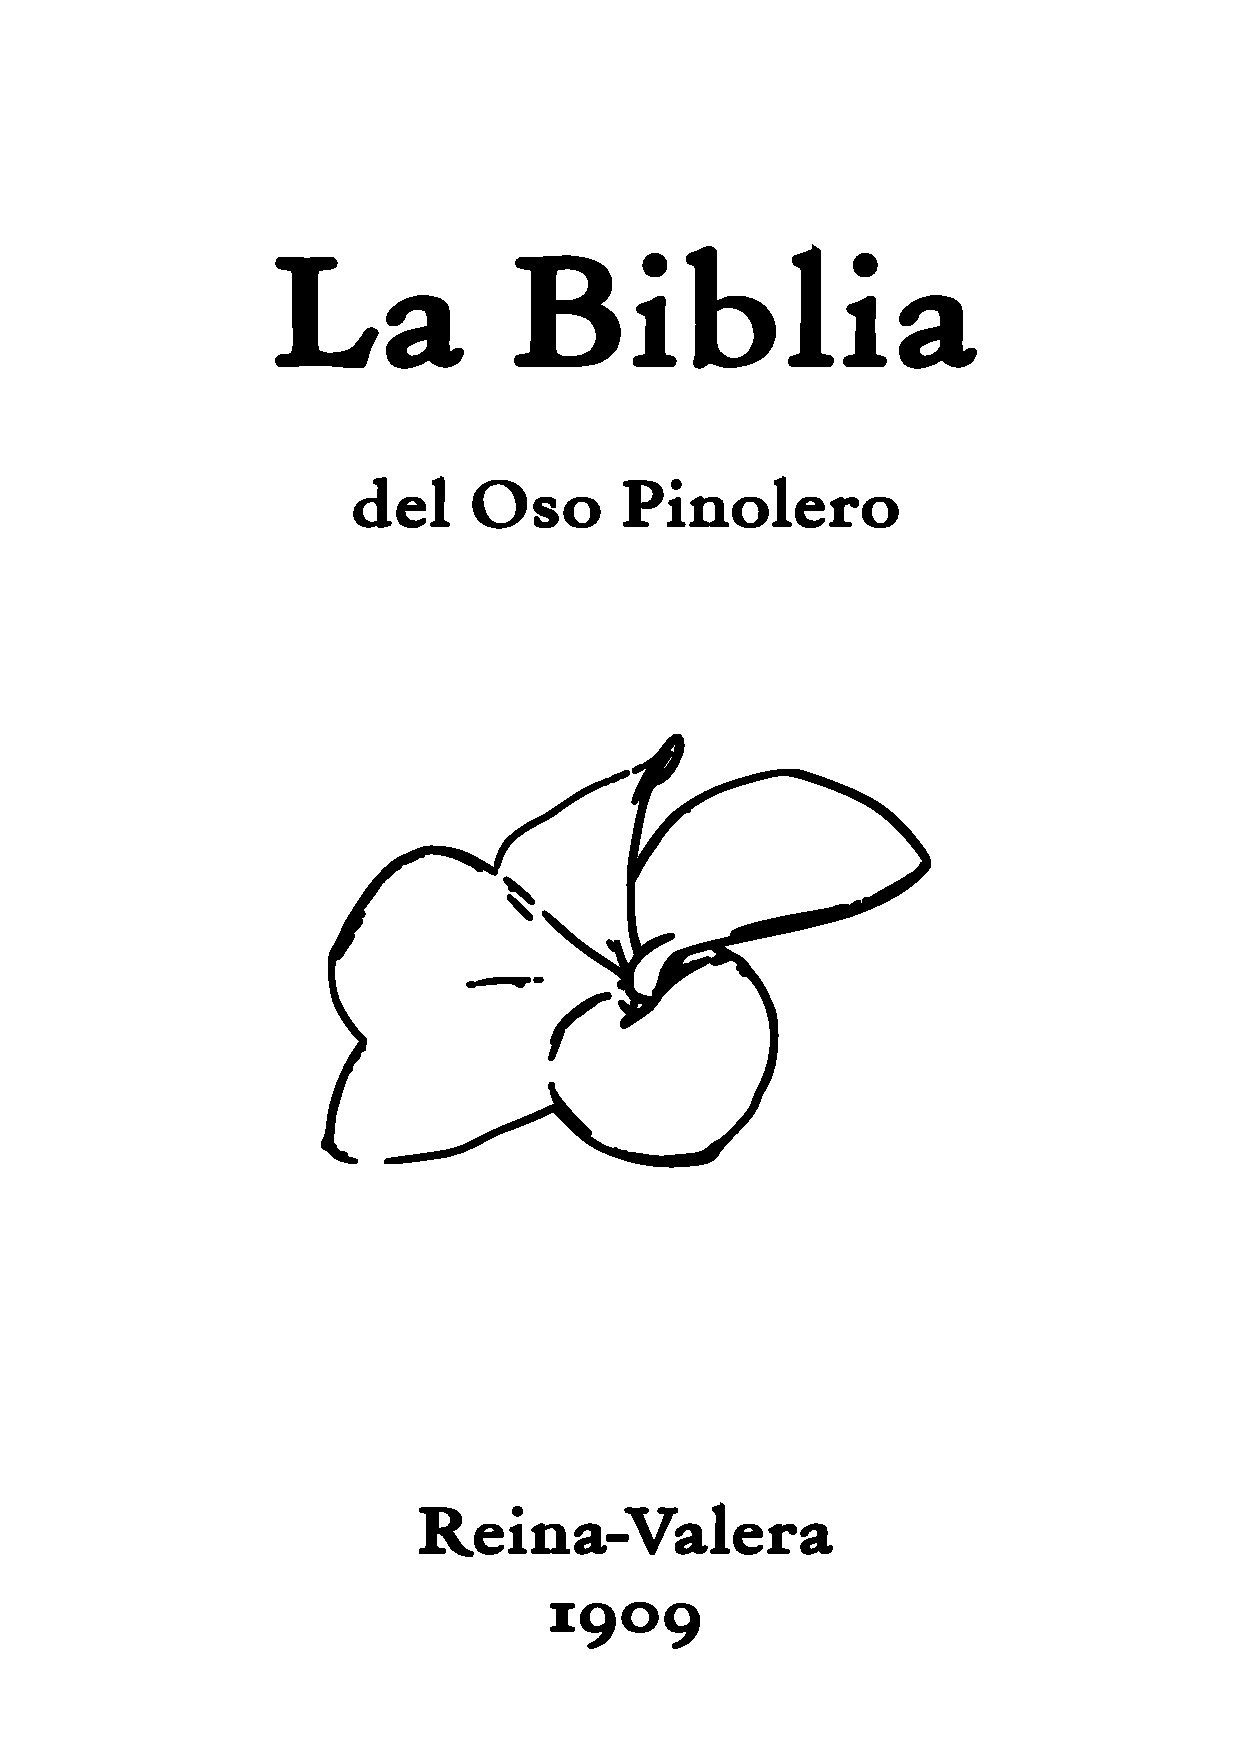
\includepdf{FrontCover.pdf}

\null\vfill
\begin{center}
\begin{minipage}[c]{\textwidth}
  \begin{center}
  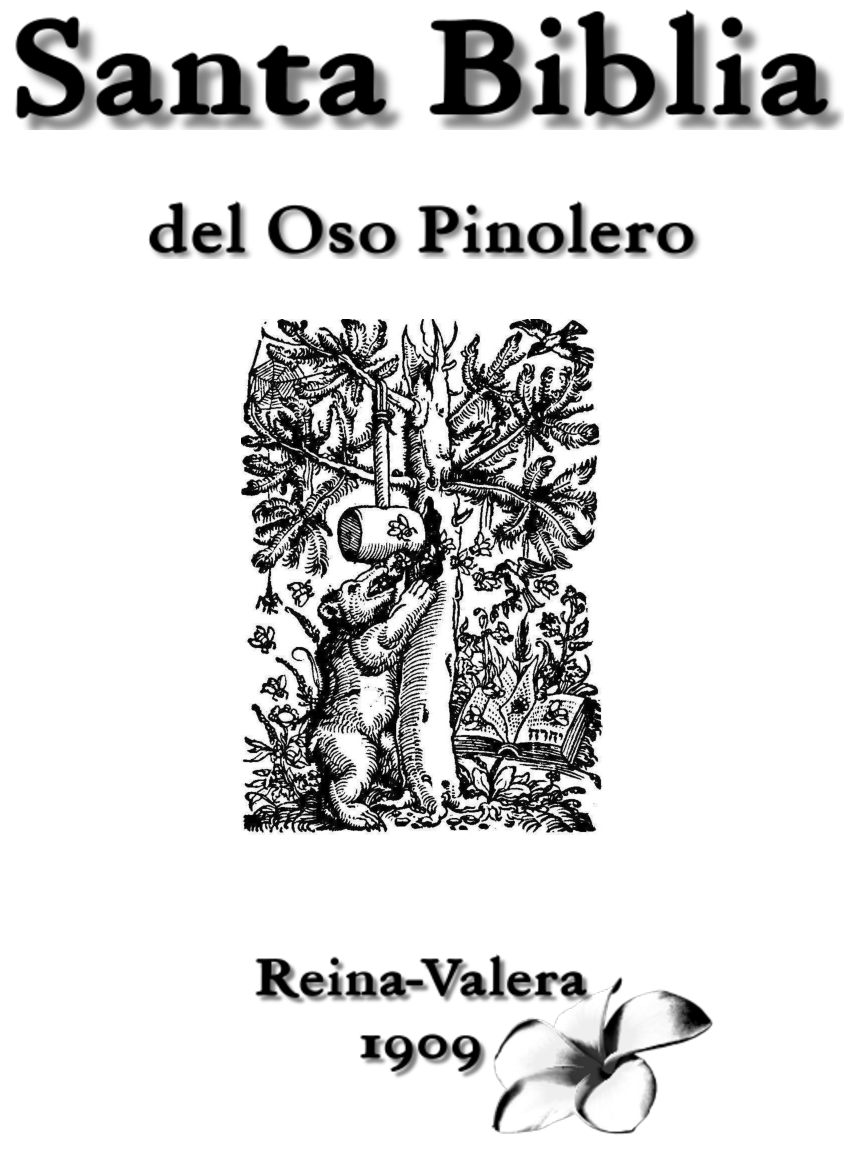
\includegraphics{Titulo.pdf}
  \end{center}
\end{minipage}
\end{center}
\newpage

\null\vfill
\noindent
Reina-Valera del Pueblo, Version 2021\\
dominio publico y fuente abierta,\\
creado por el ministerio Biblia del Pueblo\\
basado sobre el texto de la Reina-Valera 1909\\

\noindent
1ra edición 2021\\

\noindent
ISBN \dots\\

\noindent
\emph{Distribucion en Nicaragua}\\
Estrellas de Esperanza\\
Reparto santa Rosa de donde fue la hielera del yanki\\
media cuadra al sur o vien de donde es la carpinteria\\
media al sur casa color celeste\\
43000 Granada\\
Nicaragua\\
ventas@estrellasdeesperanza.org\\
www.estrellasdeesperanza.org\\

\noindent
Derechos dominio publico, el texto de la Biblia es fuente abierta\\
con una licencia de MIT.\\
El código fuente de markdown y LaTeX se encuentra en github en\\
http://www.github.com/simonegli8/FreeBible\\
Reina-Valera del Pueblo es una marca comercial registrado por Biblia del Pueblo\\
Los derechos publicar modificationes del codigo fuente abierto original con la marca Reina-Valera del Pueblo
son reservado. Si vosostro publican modificaciones del texto biblico del codigo fuente abierta original, es prohibido
utilizar la marca Reina-Valera del Pueblo, necessita cambiar el nombre de la traduccion, pero si no cambian el texto biblico es permitio. El prefacio y gloassario no son parte
del texto biblico, y se puebe modificarlo voluntariamente.\\

\noindent
Imprenta: Imprenta Jigatsa, Managua, Nicaragua\\
\newpage

\titleformat{\section}[hang]{\bfseries\huge}{}{0ex}{}[]
\input{tex/00-prefacio.tex}
\titleformat{\section}[wrap]{\bfseries\huge}{}{0ex}{}[]

\tableofcontents
\newpage

\null\vfill
\begin{center}
\begin{minipage}[c]{\textwidth}
  \begin{center}
  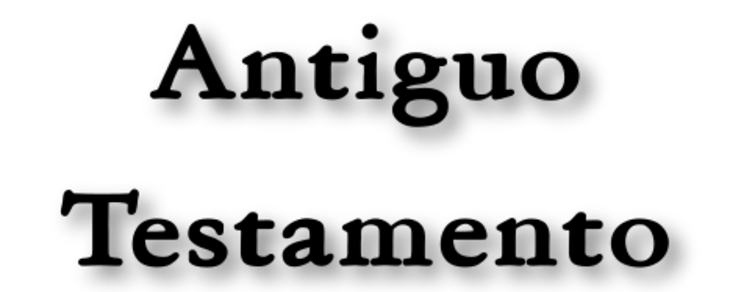
\includegraphics{AntiguoTestamentoTitulo.pdf}
  \end{center}
\end{minipage}
\end{center}
\null\vfill
\newpage

\pagestyle{bible}

\renewcommand{\cleardoublepage}{}
\renewcommand{\clearpage}{}

\chapter{Génesis}
\begin{multicols}{2}
  \input{tex/01-Génesis.tex}
\end{multicols}

\chapter{Salmos}
\begin{multicols}{2}
  \hypertarget{section}{%
\section{1}\label{section}}

\bibleverse{1} Bienaventurado el varón que no anduvo en consejo de
malos, ni estuvo en camino de pecadores, ni en silla de escarnecedores
se ha sentado; \bibleverse{2} Antes en la ley de Jehová está su delicia,
y en su ley medita de día y de noche. \bibleverse{3} Y será como el
árbol plantado junto á arroyos de aguas, que da su fruto en su tiempo, y
su hoja no cae; y todo lo que hace, prosperará. \bibleverse{4} No así
los malos: sino como el tamo que arrebata el viento. \bibleverse{5} Por
tanto no se levantarán los malos en el juicio, ni los pecadores en la
congregación de los justos. \bibleverse{6} Porque Jehová conoce el
camino de los justos; mas la senda de los malos perecerá.

\hypertarget{section-1}{%
\section{2}\label{section-1}}

\bibleverse{1} ¿Por qué se amotinan las gentes, y los pueblos piensan
vanidad? \bibleverse{2} Estarán los reyes de la tierra, y príncipes
consultarán unidos contra Jehová, y contra su ungido, diciendo:
\bibleverse{3} Rompamos sus coyundas, y echemos de nosotros sus cuerdas.
\bibleverse{4} El que mora en los cielos se reirá; el Señor se burlará
de ellos. \bibleverse{5} Entonces hablará á ellos en su furor, y
turbarálos con su ira. \bibleverse{6} Yo empero he puesto mi rey sobre
Sión, monte de mi santidad. \bibleverse{7} Yo publicaré el decreto:
Jehová me ha dicho: Mi hijo eres tú; yo te engendré hoy. \bibleverse{8}
Pídeme, y te daré por heredad las gentes, y por posesión tuya los
términos de la tierra. \bibleverse{9} Quebrantarlos has con vara de
hierro: como vaso de alfarero los desmenuzarás. \bibleverse{10} Y ahora,
reyes, entended: admitid corrección, jueces de la tierra.
\bibleverse{11} Servid á Jehová con temor, y alegraos con temblor.
\bibleverse{12} Besad al Hijo, porque no se enoje, y perezcáis en el
camino, cuando se encendiere un poco su furor. Bienaventurados todos los
que en él confían.

\hypertarget{section-2}{%
\section{3}\label{section-2}}

\bibleverse{1} Salmo de David, cuando huía de delante de Absalom su
hijo. ¡oh Jehová, cuánto se han multiplicado mis enemigos! muchos se
levantan contra mí. \bibleverse{2} Muchos dicen de mi vida: No hay para
él salud en Dios. (Selah.) \bibleverse{3} Mas tú, Jehová, eres escudo
alrededor de mí: mi gloria, y el que ensalza mi cabeza. \bibleverse{4}
Con mi voz clamé á Jehová, y él me respondió desde el monte de su
santidad. (Selah.) \bibleverse{5} Yo me acosté, y dormí, y desperté;
porque Jehová me sostuvo. \bibleverse{6} No temeré de diez millares de
pueblos, que pusieren cerco contra mí. \bibleverse{7} Levántate, Jehová;
sálvame, Dios mío: porque tú heriste á todos mis enemigos en la quijada;
los dientes de los malos quebrantaste. \bibleverse{8} De Jehová es la
salud: sobre tu pueblo será tu bendición. (Selah.)

\hypertarget{section-3}{%
\section{4}\label{section-3}}

\bibleverse{1} Al Músico principal: sobre Neginoth: Salmo de David.
Respóndeme cuando clamo, oh Dios de mi justicia: estando en angustia, tú
me hiciste ensanchar: ten misericordia de mí, y oye mi oración.
\bibleverse{2} Hijos de los hombres, ¿hasta cuándo volveréis mi honra en
infamia, amaréis la vanidad, y buscaréis la mentira? (Selah.)
\bibleverse{3} Sabed pues, que Jehová hizo apartar al pío para sí:
Jehová oirá cuando yo á él clamare. \bibleverse{4} Temblad, y no
pequéis: conversad en vuestro corazón sobre vuestra cama, y desistid.
(Selah.) \bibleverse{5} Ofreced sacrificios de justicia, y confiad en
Jehová. \bibleverse{6} Muchos dicen: ¿Quién nos mostrará el bien? Alza
sobre nosotros, oh Jehová, la luz de tu rostro. \bibleverse{7} Tú diste
alegría en mi corazón, más que tienen ellos en el tiempo que se
multiplicó su grano y su mosto. \bibleverse{8} En paz me acostaré, y
asimismo dormiré; porque solo tú, Jehová, me harás estar confiado.

\hypertarget{section-4}{%
\section{5}\label{section-4}}

\bibleverse{1} Al Músico principal: sobre Nehiloth: Salmo de David.
Escucha, oh Jehová, mis palabras; considera la meditación mía.
\bibleverse{2} Está atento á la voz de mi clamor, Rey mío y Dios mío,
porque á ti oraré. \bibleverse{3} Oh Jehová, de mañana oirás mi voz; de
mañana me presentaré á ti, y esperaré. \bibleverse{4} Porque tú no eres
un Dios que ame la maldad: el malo no habitará junto á ti.
\bibleverse{5} No estarán los insensatos delante de tus ojos: aborreces
á todos los que obran iniquidad. \bibleverse{6} Destruirás á los que
hablan mentira: al hombre de sangres y de engaño abominará Jehová.
\bibleverse{7} Y yo en la multitud de tu misericordia entraré en tu
casa: adoraré hacia el templo de tu santidad en tu temor. \bibleverse{8}
Guíame, Jehová, en tu justicia á causa de mis enemigos; endereza delante
de mí tu camino. \bibleverse{9} Porque no hay en su boca rectitud: sus
entrañas son pravedades; sepulcro abierto su garganta: con su lengua
lisonjearán. \bibleverse{10} Desbarátalos, oh Dios; caigan de sus
consejos: por la multitud de sus rebeliones échalos, porque se rebelaron
contra ti. \bibleverse{11} Y alegrarse han todos los que en ti confían;
para siempre darán voces de júbilo, porque tú los defiendes: y en ti se
regocijarán los que aman tu nombre. \bibleverse{12} Porque tú, oh
Jehová, bendecirás al justo; lo cercarás de benevolencia como con un
escudo.

\hypertarget{section-5}{%
\section{6}\label{section-5}}

\bibleverse{1} Al Músico principal: en Neginoth sobre Seminith: Salmo de
David. Jehová, no me reprendas en tu furor, ni me castigues con tu ira.
\bibleverse{2} Ten misericordia de mí, oh Jehová, porque yo estoy
debilitado: sáname, oh Jehová, porque mis huesos están conmovidos.
\bibleverse{3} Mi alma asimismo está muy conturbada: y tú, Jehová,
¿hasta cuándo? \bibleverse{4} Vuelve, oh Jehová, libra mi alma; sálvame
por tu misericordia. \bibleverse{5} Porque en la muerte no hay memoria
de ti: ¿quién te loará en el sepulcro? \bibleverse{6} Heme consumido á
fuerza de gemir: todas las noches inundo mi lecho, riego mi estrado con
mis lágrimas. \bibleverse{7} Mis ojos están carcomidos de descontento;
hanse envejecido á causa de todos mis angustiadores. \bibleverse{8}
Apartaos de mí, todos los obradores de iniquidad; porque Jehová ha oído
la voz de mi lloro. \bibleverse{9} Jehová ha oído mi ruego; ha recibido
Jehová mi oración. \bibleverse{10} Se avergonzarán, y turbaránse mucho
todos mis enemigos; volveránse y serán avergonzados subitáneamente.

\hypertarget{section-6}{%
\section{7}\label{section-6}}

\bibleverse{1} Sigaión de David, que cantó á Jehová sobre las palabras
de Cus, hijo de Benjamín. Jehová Dios mío, en ti he confiado: sálvame de
todos los que me persiguen, y líbrame; \bibleverse{2} No sea que
arrebate mi alma, cual león que despedaza, sin que haya quien libre.
\bibleverse{3} Jehová Dios mío, si yo he hecho esto, si hay en mis manos
iniquidad; \bibleverse{4} Si dí mal pago al pacífico conmigo, (hasta he
libertado al que sin causa era mi enemigo;) \bibleverse{5} Persiga el
enemigo mi alma, y alcáncela; y pise en tierra mi vida, y mi honra ponga
en el polvo. (Selah.) \bibleverse{6} Levántate, oh Jehová, con tu furor;
álzate á causa de las iras de mis angustiadores, y despierta en favor
mío el juicio que mandaste. \bibleverse{7} Y te rodeará concurso de
pueblo; por cuyo amor vuélvete luego á levantar en alto. \bibleverse{8}
Jehová juzgará los pueblos: júzgame, oh Jehová, conforme á mi justicia y
conforme á mi integridad. \bibleverse{9} Consúmase ahora la malicia de
los inicuos, y establece al justo; pues el Dios justo prueba los
corazones y los riñones. \bibleverse{10} Mi escudo está en Dios, que
salva á los rectos de corazón. \bibleverse{11} Dios es el que juzga al
justo: y Dios está airado todos los días contra el impío.
\bibleverse{12} Si no se convirtiere, él afilará su espada: armado tiene
ya su arco, y lo ha preparado. \bibleverse{13} Asimismo ha aparejado
para él armas de muerte; ha labrado sus saetas para los que persiguen.
\bibleverse{14} He aquí ha tenido parto de iniquidad: concibió trabajo,
y parió mentira. \bibleverse{15} Pozo ha cavado, y ahondádolo; y en la
fosa que hizo caerá. \bibleverse{16} Su trabajo se tornará sobre su
cabeza, y su agravio descenderá sobre su mollera. \bibleverse{17}
Alabaré yo á Jehová conforme á su justicia, y cantaré al nombre de
Jehová el Altísimo.

\hypertarget{section-7}{%
\section{8}\label{section-7}}

\bibleverse{1} Al Músico principal: sobre Gittith: Salmo de David. Oh
Jehová, Señor nuestro, ¡cuán grande es tu nombre en toda la tierra, que
has puesto tu gloria sobre los cielos! \bibleverse{2} De la boca de los
chiquitos y de los que maman, fundaste la fortaleza, á causa de tus
enemigos, para hacer cesar al enemigo, y al que se venga. \bibleverse{3}
Cuando veo tus cielos, obra de tus dedos, la luna y las estrellas que tú
formaste: \bibleverse{4} Digo: ¿Qué es el hombre, para que tengas de él
memoria, y el hijo del hombre, que lo visites? \bibleverse{5} Pues le
has hecho poco menor que los ángeles, y coronástelo de gloria y de
lustre. \bibleverse{6} Hicístelo enseñorear de las obras de tus manos;
todo lo pusiste debajo de sus pies: \bibleverse{7} Ovejas, y bueyes,
todo ello; y asimismo las bestias del campo; \bibleverse{8} Las aves de
los cielos, y los peces de la mar; todo cuanto pasa por los senderos de
la mar. \bibleverse{9} Oh Jehová, Señor nuestro, ¡cuán grande es tu
nombre en toda la tierra!

\hypertarget{section-8}{%
\section{9}\label{section-8}}

\bibleverse{1} Al Músico principal: sobre Muth-labben: Salmo de David.
Te alabaré, oh Jehová, con todo mi corazón; contaré todas tus
maravillas. \bibleverse{2} Alegraréme y regocijaréme en ti: cantaré á tu
nombre, oh Altísimo; \bibleverse{3} Por haber sido mis enemigos vueltos
atrás: caerán y perecerán delante de ti. \bibleverse{4} Porque has hecho
mi juicio y mi causa: sentástete en silla juzgando justicia.
\bibleverse{5} Reprendiste gentes, destruiste al malo, raíste el nombre
de ellos para siempre jamás. \bibleverse{6} Oh enemigo, acabados son
para siempre los asolamientos; y las ciudades que derribaste, su memoria
pereció con ellas. \bibleverse{7} Mas Jehová permanecerá para siempre:
dispuesto ha su trono para juicio. \bibleverse{8} Y él juzgará el mundo
con justicia; y juzgará los pueblos con rectitud. \bibleverse{9} Y será
Jehová refugio al pobre, refugio para el tiempo de angustia.
\bibleverse{10} Y en ti confiarán los que conocen tu nombre; por cuanto
tú, oh Jehová, no desamparaste á los que te buscaron. \bibleverse{11}
Cantad á Jehová, que habita en Sión: noticiad en los pueblos sus obras.
\bibleverse{12} Porque demandando la sangre se acordó de ellos: no se
olvidó del clamor de los pobres. \bibleverse{13} Ten misericordia de mí,
Jehová: mira mi aflicción que padezco de los que me aborrecen, tú que me
levantas de las puertas de la muerte; \bibleverse{14} Porque cuente yo
todas tus alabanzas en las puertas de la hija de Sión, y me goce en tu
salud. \bibleverse{15} Hundiéronse las gentes en la fosa que hicieron;
en la red que escondieron fué tomado su pie. \bibleverse{16} Jehová fué
conocido en el juicio que hizo; en la obra de sus manos fué enlazado el
malo. (Higaion. Selah.) \bibleverse{17} Los malos serán trasladados al
infierno, todas las gentes que se olvidan de Dios. \bibleverse{18}
Porque no para siempre será olvidado el pobre; ni la esperanza de los
pobres perecerá perpetuamente. \bibleverse{19} Levántate, oh Jehová; no
se fortalezca el hombre; sean juzgadas las gentes delante de ti.
\bibleverse{20} Pon, oh Jehová, temor en ellos: conozcan las gentes que
son no más que hombres. (Selah.)

\hypertarget{section-9}{%
\section{10}\label{section-9}}

\bibleverse{1} ¿Por qué estás lejos, oh Jehová, y te escondes en el
tiempo de la tribulación? \bibleverse{2} Con arrogancia el malo persigue
al pobre: serán cogidos en los artificios que han ideado. \bibleverse{3}
Por cuanto se alaba el malo del deseo de su alma, y bendice al
codicioso, á quien Jehová aborrece. \bibleverse{4} El malo, por la
altivez de su rostro, no busca á Dios: no hay Dios en todos sus
pensamientos. \bibleverse{5} Sus caminos son viciosos en todo tiempo:
tus juicios los tiene muy lejos de su vista: echa bocanadas en orden á
todos sus enemigos. \bibleverse{6} Dice en su corazón: No seré movido en
ningún tiempo, ni jamás me alcanzará el infortunio. \bibleverse{7} Llena
está su boca de maldición, y de engaños y fraude: debajo de su lengua,
vejación y maldad. \bibleverse{8} Está en las guaridas de las aldeas: en
los escondrijos mata al inocente: sus ojos están acechando al pobre.
\bibleverse{9} Acecha en oculto, como el león desde su cama: acecha para
arrebatar al pobre: arrebata al pobre trayéndolo á su red.
\bibleverse{10} Encógese, agáchase, y caen en sus fuerzas muchos
desdichados. \bibleverse{11} Dice en su corazón: Dios está olvidado, ha
encubierto su rostro; nunca lo verá. \bibleverse{12} Levántate, oh
Jehová Dios, alza tu mano, no te olvides de los pobres. \bibleverse{13}
¿Por qué irrita el malo á Dios? En su corazón ha dicho que no lo
inquirirás. \bibleverse{14} Tú lo tienes visto: porque tú miras el
trabajo, y la vejación, para vengarle por tu mano: á ti se acoge el
pobre, tú eres el amparo del huérfano. \bibleverse{15} Quebranta el
brazo del malo: del maligno buscarás su maldad, hasta que ninguna
halles. \bibleverse{16} Jehová, Rey eterno y perpetuo; de su tierra
fueron destruídas las gentes. \bibleverse{17} El deseo de los humildes
oíste, oh Jehová: tú dispones su corazón, y haces atento tu oído;
\bibleverse{18} Para juzgar al huérfano y al pobre, á fin de que no
vuelva más á hacer violencia el hombre de la tierra.

\hypertarget{section-10}{%
\section{11}\label{section-10}}

\bibleverse{1} Al Músico principal: Salmo de David. En Jehová he
confiado; ¿cómo decís á mi alma: Escapa al monte cual ave?
\bibleverse{2} Porque he aquí, los malos flecharon el arco, apercibieron
sus saetas sobre la cuerda, para asaetear en oculto á los rectos de
corazón. \bibleverse{3} Si fueren destruídos los fundamentos, ¿qué ha de
hacer el justo? \bibleverse{4} Jehová en el templo de su santidad: la
silla de Jehová está en el cielo: sus ojos ven, sus párpados examinan á
los hijos de los hombres. \bibleverse{5} Jehová prueba al justo; empero
al malo y al que ama la violencia, su alma aborrece. \bibleverse{6}
Sobre los malos lloverá lazos; fuego y azufre, con vientos de
torbellinos, será la porción del cáliz de ellos. \bibleverse{7} Porque
el justo Jehová ama la justicia: al recto mirará su rostro.

\hypertarget{section-11}{%
\section{12}\label{section-11}}

\bibleverse{1} Al Músico principal: sobre Seminith: Salmo de David.
Salva, oh Jehová, porque se acabaron los misericordiosos: porque se han
acabado los fieles de entre los hijos de los hombres. \bibleverse{2}
Mentira habla cada uno con su prójimo; con labios lisonjeros, con
corazón doble hablan. \bibleverse{3} Destruirá Jehová todos los labios
lisonjeros, la lengua que habla grandezas; \bibleverse{4} Que dijeron:
Por nuestra lengua prevaleceremos; nuestros labios están con nosotros:
¿quién nos es señor? \bibleverse{5} Por la opresión de los pobres, por
el gemido de los menesterosos, ahora me levantaré, dice Jehová:
pondrélos en salvo del que contra ellos se engríe. \bibleverse{6} Las
palabras de Jehová, palabras limpias; plata refinada en horno de tierra,
purificada siete veces. \bibleverse{7} Tú, Jehová, los guardarás;
guárdalos para siempre de aquesta generación. \bibleverse{8} Cercando
andan los malos, mientras son exaltados los más viles de los hijos de
los hombres.

\hypertarget{section-12}{%
\section{13}\label{section-12}}

\bibleverse{1} Al Músico principal: Salmo de David. ¿hasta cuándo,
Jehová? ¿me olvidarás para siempre? ¿hasta cuándo esconderás tu rostro
de mí? \bibleverse{2} ¿Hasta cuándo pondré consejos en mi alma, con
ansiedad en mi corazón cada día? ¿Hasta cuándo será enaltecido mi
enemigo sobre mí? \bibleverse{3} Mira, óyeme, Jehová Dios mío: alumbra
mis ojos, porque no duerma en muerte; \bibleverse{4} Porque no diga mi
enemigo, Vencílo: mis enemigos se alegrarán, si yo resbalare.
\bibleverse{5} Mas yo en tu misericordia he confiado: alegraráse mi
corazón en tu salud. \bibleverse{6} Cantaré á Jehová, porque me ha hecho
bien.

\hypertarget{section-13}{%
\section{14}\label{section-13}}

\bibleverse{1} Al Músico principal: Salmo de David. Dijo el necio en su
corazón: No hay Dios. Corrompiéronse, hicieron obras abominables; no hay
quien haga bien. \bibleverse{2} Jehová miró desde los cielos sobre los
hijos de los hombres, por ver si había algún entendido, que buscara á
Dios. \bibleverse{3} Todos declinaron, juntamente se han corrompido: no
hay quien haga bien, no hay ni siquiera uno. \bibleverse{4} ¿No tendrán
conocimiento todos los que obran iniquidad, que devoran á mi pueblo como
si pan comiesen, y á Jehová no invocaron? \bibleverse{5} Allí temblaron
de espanto; porque Dios está con la nación de los justos. \bibleverse{6}
El consejo del pobre habéis escarnecido, por cuanto Jehová es su
esperanza. \bibleverse{7} ¡Quién diese de Sión la salud de Israel! En
tornando Jehová la cautividad de su pueblo, se gozará Jacob, y
alegraráse Israel.

\hypertarget{section-14}{%
\section{15}\label{section-14}}

\bibleverse{1} Salmo de David. Jehová, ¿quién habitará en tu
tabernáculo? ¿quién residirá en el monte de tu santidad? \bibleverse{2}
El que anda en integridad, y obra justicia, y habla verdad en su
corazón. \bibleverse{3} El que no detrae con su lengua, ni hace mal á su
prójimo, ni contra su prójimo acoge oprobio alguno. \bibleverse{4} Aquel
á cuyos ojos es menospreciado el vil; mas honra á los que temen á
Jehová: y habiendo jurado en daño suyo, no por eso muda. \bibleverse{5}
Quien su dinero no dió á usura, ni contra el inocente tomó cohecho. El
que hace estas cosas, no resbalará para siempre.

\hypertarget{section-15}{%
\section{16}\label{section-15}}

\bibleverse{1} Michtham de David. Guárdame, oh Dios, porque en ti he
confiado. \bibleverse{2} Dijiste, oh alma mía, á Jehová: Tú eres el
Señor: mi bien á ti no aprovecha; \bibleverse{3} Sino á los santos que
están en la tierra, y á los íntegros: toda mi afición en ellos.
\bibleverse{4} Multiplicaránse los dolores de aquellos que sirven
diligentes á otro dios: no ofreceré yo sus libaciones de sangre, ni en
mis labios tomaré sus nombres. \bibleverse{5} Jehová es la porción de mi
parte y de mi copa; tú sustentarás mi suerte. \bibleverse{6} Las cuerdas
me cayeron en lugares deleitosos, y es hermosa la heredad que me ha
tocado. \bibleverse{7} Bendeciré á Jehová que me aconseja: aun en las
noches me enseñan mis riñones. \bibleverse{8} A Jehová he puesto siempre
delante de mí: porque está á mi diestra no seré conmovido.
\bibleverse{9} Alegróse por tanto mi corazón, y se gozó mi gloria:
también mi carne reposará segura. \bibleverse{10} Porque no dejarás mi
alma en el sepulcro; ni permitirás que tu santo vea corrupción.
\bibleverse{11} Me mostrarás la senda de la vida: hartura de alegrías
hay con tu rostro; deleites en tu diestra para siempre.

\hypertarget{section-16}{%
\section{17}\label{section-16}}

\bibleverse{1} Oración de David. Oye, oh Jehová, justicia; está atento á
mi clamor; escucha mi oración hecha sin labios de engaño. \bibleverse{2}
De delante de tu rostro salga mi juicio; vean tus ojos la rectitud.
\bibleverse{3} Tú has probado mi corazón, hasme visitado de noche; me
has apurado, y nada inicuo hallaste: heme propuesto que mi boca no ha de
propasarse. \bibleverse{4} Para las obras humanas, por la palabra de tus
labios yo me he guardado de las vías del destructor. \bibleverse{5}
Sustenta mis pasos en tus caminos, porque mis pies no resbalen.
\bibleverse{6} Yo te he invocado, por cuanto tú me oirás, oh Dios:
inclina á mí tu oído, escucha mi palabra. \bibleverse{7} Muestra tus
estupendas misericordias, tú que salvas á los que en ti confían de los
que se levantan contra tu diestra. \bibleverse{8} Guárdame como lo negro
de la niñeta del ojo, escóndeme con la sombra de tus alas,
\bibleverse{9} De delante de los malos que me oprimen, de mis enemigos
que me cercan por la vida. \bibleverse{10} Cerrados están con su
grosura; con su boca hablan soberbiamente. \bibleverse{11} Nuestros
pasos nos han cercado ahora: puestos tienen sus ojos para echarnos por
tierra. \bibleverse{12} Parecen al león que desea hacer presa, y al
leoncillo que está escondido. \bibleverse{13} Levántate, oh Jehová;
prevén su encuentro, póstrale: libra mi alma del malo con tu espada;
\bibleverse{14} De los hombres con tu mano, oh Jehová, de los hombres de
mundo, cuya parte es en esta vida, y cuyo vientre hinches de tu tesoro:
hartan sus hijos, y dejan el resto á sus chiquitos. \bibleverse{15} Yo
en justicia veré tu rostro: seré saciado cuando despertare á tu
semejanza.

\hypertarget{section-17}{%
\section{18}\label{section-17}}

\bibleverse{1} Al Músico principal: Salmo de David, siervo de Jehová, el
cual profirió á Jehová las palabras de este cántico el día que le libró
Jehová de mano de todos sus enemigos, y de mano de Saúl. Entonces dijo:
Amarte he, oh Jehová, fortaleza mía. \bibleverse{2} Jehová, roca mía y
castillo mío, y mi libertador; Dios mío, fuerte mío, en él confiaré;
escudo mío, y el cuerno de mi salud, mi refugio. \bibleverse{3} Invocaré
á Jehová, digno de ser alabado, y seré salvo de mis enemigos.
\bibleverse{4} Cercáronme dolores de muerte, y torrentes de perversidad
me atemorizaron. \bibleverse{5} Dolores del sepulcro me rodearon,
previniéronme lazos de muerte. \bibleverse{6} En mi angustia invoqué á
Jehová, y clamé á mi Dios: él oyó mi voz desde su templo, y mi clamor
llegó delante de él, á sus oídos. \bibleverse{7} Y la tierra fué
conmovida y tembló; y moviéronse los fundamentos de los montes, y se
estremecieron, porque se indignó él. \bibleverse{8} Humo subió de su
nariz, y de su boca consumidor fuego; carbones fueron por él encendidos.
\bibleverse{9} Y bajó los cielos, y descendió; y oscuridad debajo de sus
pies. \bibleverse{10} Y cabalgó sobre un querubín, y voló: voló sobre
las alas del viento. \bibleverse{11} Puso tinieblas por escondedero
suyo, su pabellón en derredor de sí; oscuridad de aguas, nubes de los
cielos. \bibleverse{12} Por el resplandor delante de él, sus nubes
pasaron; granizo y carbones ardientes. \bibleverse{13} Y tronó en los
cielos Jehová, y el Altísimo dió su voz; granizo y carbones de fuego.
\bibleverse{14} Y envió sus saetas, y desbaratólos; y echó relámpagos, y
los destruyó. \bibleverse{15} Y aparecieron las honduras de las aguas, y
descubriéronse los cimientos del mundo, á tu reprensión, oh Jehová, por
el soplo del viento de tu nariz. \bibleverse{16} Envió desde lo alto;
tomóme, sacóme de las muchas aguas. \bibleverse{17} Libróme de mi
poderoso enemigo, y de los que me aborrecían, aunque eran ellos más
fuertes que yo. \bibleverse{18} Asaltáronme en el día de mi quebranto:
mas Jehová fué mi apoyo. \bibleverse{19} Y sacóme á anchura: libróme,
porque se agradó de mí. \bibleverse{20} Hame pagado Jehová conforme á mi
justicia: conforme á la limpieza de mis manos me ha vuelto.
\bibleverse{21} Porque yo he guardado los caminos de Jehová, y no me
aparté impíamente de mi Dios. \bibleverse{22} Pues todos sus juicios
estuvieron delante de mí, y no eché de mí sus estatutos. \bibleverse{23}
Y fuí íntegro para con él, y cauteléme de mi maldad. \bibleverse{24}
Pagóme pues Jehová conforme á mi justicia; conforme á la limpieza de mis
manos delante de sus ojos. \bibleverse{25} Con el misericordioso te
mostrarás misericordioso, y recto para con el hombre íntegro.
\bibleverse{26} Limpio te mostrarás para con el limpio, y severo serás
para con el perverso. \bibleverse{27} Y tú salvarás al pueblo humilde, y
humillarás los ojos altivos. \bibleverse{28} Tú pues alumbrarás mi
lámpara: Jehová mi Dios alumbrará mis tinieblas. \bibleverse{29} Porque
contigo desharé ejércitos; y con mi Dios asaltaré muros. \bibleverse{30}
Dios, perfecto su camino: es acendrada la palabra de Jehová: escudo es á
todos los que en él esperan. \bibleverse{31} Porque ¿qué Dios hay fuera
de Jehová? ¿y qué fuerte fuera de nuestro Dios? \bibleverse{32} Dios es
el que me ciñe de fuerza, é hizo perfecto mi camino; \bibleverse{33}
Quien pone mis pies como pies de ciervas, é hízome estar sobre mis
alturas; \bibleverse{34} Quien enseña mis manos para la batalla, y será
quebrado con mis brazos el arco de acero. \bibleverse{35} Dísteme
asimismo el escudo de tu salud: y tu diestra me sustentó, y tu
benignidad me ha acrecentado. \bibleverse{36} Ensanchaste mis pasos
debajo de mí, y no titubearon mis rodillas. \bibleverse{37} Perseguido
he mis enemigos, y alcancélos, y no volví hasta acabarlos.
\bibleverse{38} Helos herido, y no podrán levantarse: cayeron debajo de
mis pies. \bibleverse{39} Pues me ceñiste de fortaleza para la pelea;
has agobiado mis enemigos debajo de mí. \bibleverse{40} Y dísteme la
cerviz de mis enemigos, y destruí á los que me aborrecían.
\bibleverse{41} Clamaron, y no hubo quien salvase: aun á Jehová, mas no
los oyó. \bibleverse{42} Y molílos como polvo delante del viento;
esparcílos como lodo de las calles. \bibleverse{43} Librásteme de
contiendas de pueblo: pusísteme por cabecera de gentes: pueblo que yo no
conocía, me sirvió. \bibleverse{44} Así que hubo oído, me obedeció; los
hijos de extraños me mintieron; \bibleverse{45} Los extraños flaquearon,
y tuvieron miedo desde sus encerramientos. \bibleverse{46} Viva Jehová,
y sea bendita mi roca; y ensalzado sea el Dios de mi salud:
\bibleverse{47} El Dios que me da las venganzas, y sujetó pueblos á mí.
\bibleverse{48} Mi libertador de mis enemigos: hicísteme también
superior de mis adversarios; librásteme de varón violento.
\bibleverse{49} Por tanto yo te confesaré entre las gentes, oh Jehová, y
cantaré á tu nombre. \bibleverse{50} El cual engrandece las saludes de
su rey, y hace misericordia á su ungido, á David y á su simiente, para
siempre.

\hypertarget{section-18}{%
\section{19}\label{section-18}}

\bibleverse{1} Al Músico principal: Salmo de David. Los cielos cuentan
la gloria de Dios, y la expansión denuncia la obra de sus manos.
\bibleverse{2} El un día emite palabra al otro día, y la una noche á la
otra noche declara sabiduría. \bibleverse{3} No hay dicho, ni palabras,
ni es oída su voz. \bibleverse{4} Por toda la tierra salió su hilo, y al
cabo del mundo sus palabras. En ellos puso tabernáculo para el sol.
\bibleverse{5} Y él, como un novio que sale de su tálamo, alégrase cual
gigante para correr el camino. \bibleverse{6} Del un cabo de los cielos
es su salida, y su giro hasta la extremidad de ellos: y no hay quien se
esconda de su calor. \bibleverse{7} La ley de Jehová es perfecta, que
vuelve el alma: el testimonio de Jehová, fiel, que hace sabio al
pequeño. \bibleverse{8} Los mandamientos de Jehová son rectos, que
alegran el corazón: el precepto de Jehová, puro, que alumbra los ojos.
\bibleverse{9} El temor de Jehová, limpio, que permanece para siempre;
los juicios de Jehová son verdad, todos justos. \bibleverse{10}
Deseables son más que el oro, y más que mucho oro afinado; y dulces más
que miel, y que la que destila del panal. \bibleverse{11} Tu siervo es
además amonestado con ellos: en guardarlos hay grande galardón.
\bibleverse{12} Los errores, ¿quién los entenderá? Líbrame de los que me
son ocultos. \bibleverse{13} Detén asimismo á tu siervo de las
soberbias; que no se enseñoreen de mí: entonces seré íntegro, y estaré
limpio de gran rebelión. \bibleverse{14} Sean gratos los dichos de mi
boca y la meditación de mi corazón delante de ti, oh Jehová, roca mía, y
redentor mío.

\hypertarget{section-19}{%
\section{20}\label{section-19}}

\bibleverse{1} Al Músico principal: Salmo de David. Oigate Jehová en el
día de conflicto; defiéndate el nombre del Dios de Jacob. \bibleverse{2}
Envíete ayuda desde el santuario, y desde Sión te sostenga.
\bibleverse{3} Haga memoria de todos tus presentes, y reduzca á ceniza
tu holocausto. (Selah.) \bibleverse{4} Déte conforme á tu corazón, y
cumpla todo tu consejo. \bibleverse{5} Nosotros nos alegraremos por tu
salud, y alzaremos pendón en el nombre de nuestro Dios: cumpla Jehová
todas tus peticiones. \bibleverse{6} Ahora echo de ver que Jehová guarda
á su ungido: oirálo desde los cielos de su santidad, con la fuerza de la
salvación de su diestra. \bibleverse{7} Estos confían en carros, y
aquéllos en caballos: mas nosotros del nombre de Jehová nuestro Dios
tendremos memoria. \bibleverse{8} Ellos arrodillaron, y cayeron; mas
nosotros nos levantamos, y nos enhestamos. \bibleverse{9} Salva, Jehová:
que el Rey nos oiga el día que lo invocáremos.

\hypertarget{section-20}{%
\section{21}\label{section-20}}

\bibleverse{1} Al Músico principal: Salmo de David. Alegraráse el rey en
tu fortaleza, oh Jehová; y en tu salud se gozará mucho. \bibleverse{2}
El deseo de su corazón le diste, y no le negaste lo que sus labios
pronunciaron. (Selah.) \bibleverse{3} Pues le has salido al encuentro
con bendiciones de bien: corona de oro fino has puesto sobre su cabeza.
\bibleverse{4} Vida te demandó, y dístele largura de días por siglos y
siglos. \bibleverse{5} Grande es su gloria en tu salud: honra y majestad
has puesto sobre él. \bibleverse{6} Porque lo has bendecido para
siempre; llenástelo de alegría con tu rostro. \bibleverse{7} Por cuanto
el rey confía en Jehová, y en la misericordia del Altísimo, no será
conmovido. \bibleverse{8} Alcanzará tu mano á todos tus enemigos; tu
diestra alcanzará á los que te aborrecen. \bibleverse{9} Ponerlos has
como horno de fuego en el tiempo de tu ira: Jehová los deshará en su
furor, y fuego los consumirá. \bibleverse{10} Su fruto destruirás de la
tierra, y su simiente de entre los hijos de los hombres. \bibleverse{11}
Porque trazaron el mal contra ti: fraguaron maquinaciones, mas no
prevalecerán. \bibleverse{12} Pues tú los pondrás en fuga, cuando
aparejares en tus cuerdas las saetas contra sus rostros. \bibleverse{13}
Ensálzate, oh Jehová, con tu fortaleza: cantaremos y alabaremos tu
poderío.

\hypertarget{section-21}{%
\section{22}\label{section-21}}

\bibleverse{1} Al Músico principal, sobre Ajeleth-sahar: Salmo de David.
Dios mío, Dios mío, ¿por qué me has dejado? ¿por qué estás lejos de mi
salud, y de las palabras de mi clamor? \bibleverse{2} Dios mío, clamo de
día, y no oyes; y de noche, y no hay para mí silencio. \bibleverse{3} Tú
empero eres santo, tú que habitas entre las alabanzas de Israel.
\bibleverse{4} En ti esperaron nuestros padres: esperaron, y tú los
libraste. \bibleverse{5} Clamaron á ti, y fueron librados: esperaron en
ti, y no se avergonzaron. \bibleverse{6} Mas yo soy gusano, y no hombre;
oprobio de los hombres, y desecho del pueblo. \bibleverse{7} Todos los
que me ven, escarnecen de mí; estiran los labios, menean la cabeza,
diciendo: \bibleverse{8} Remítese á Jehová, líbrelo; sálvele, puesto que
en él se complacía. \bibleverse{9} Empero tú eres el que me sacó del
vientre, el que me haces esperar desde que estaba á los pechos de mi
madre. \bibleverse{10} Sobre ti fuí echado desde la matriz: desde el
vientre de mi madre, tú eres mi Dios. \bibleverse{11} No te alejes de
mí, porque la angustia está cerca; porque no hay quien ayude.
\bibleverse{12} Hanme rodeado muchos toros; fuertes toros de Basán me
han cercado. \bibleverse{13} Abrieron sobre mí su boca, como león
rapante y rugiente. \bibleverse{14} Heme escurrido como aguas, y todos
mis huesos se descoyuntaron: mi corazón fué como cera, desliéndose en
medio de mis entrañas. \bibleverse{15} Secóse como un tiesto mi vigor, y
mi lengua se pegó á mi paladar; y me has puesto en el polvo de la
muerte. \bibleverse{16} Porque perros me han rodeado, hame cercado
cuadrilla de malignos: horadaron mis manos y mis pies. \bibleverse{17}
Contar puedo todos mis huesos; ellos miran, considéranme.
\bibleverse{18} Partieron entre sí mis vestidos, y sobre mi ropa echaron
suertes. \bibleverse{19} Mas tú, Jehová, no te alejes; fortaleza mía,
apresúrate para mi ayuda. \bibleverse{20} Libra de la espada mi alma;
del poder del perro mi única. \bibleverse{21} Sálvame de la boca del
león, y óyeme librándome de los cuernos de los unicornios.
\bibleverse{22} Anunciaré tu nombre á mis hermanos: en medio de la
congregación te alabaré. \bibleverse{23} Los que teméis á Jehová,
alabadle; glorificadle, simiente toda de Jacob; y temed de él, vosotros,
simiente toda de Israel. \bibleverse{24} Porque no menospreció ni
abominó la aflicción del pobre, ni de él escondió su rostro; sino que
cuando clamó á él, oyóle. \bibleverse{25} De ti será mi alabanza en la
grande congregación; mis votos pagaré delante de los que le temen.
\bibleverse{26} Comerán los pobres, y serán saciados: alabarán á Jehová
los que le buscan: vivirá vuestro corazón para siempre. \bibleverse{27}
Acordarse han, y volveránse á Jehová todos los términos de la tierra; y
se humillarán delante de ti todas las familias de las gentes.
\bibleverse{28} Porque de Jehová es el reino; y él se enseñoreará de las
gentes. \bibleverse{29} Comerán y adorarán todos los poderosos de la
tierra: postraránse delante de él todos los que descienden al polvo, si
bien ninguno puede conservar la vida á su propia alma. \bibleverse{30}
La posteridad le servirá; será ella contada por una generación de
Jehová. \bibleverse{31} Vendrán, y anunciarán al pueblo que naciere, su
justicia que él hizo.

\hypertarget{section-22}{%
\section{23}\label{section-22}}

\bibleverse{1} Salmo de David. Jehová es mi pastor; nada me faltará.
\bibleverse{2} En lugares de delicados pastos me hará yacer: junto á
aguas de reposo me pastoreará. \bibleverse{3} Confortará mi alma;
guiaráme por sendas de justicia por amor de su nombre. \bibleverse{4}
Aunque ande en valle de sombra de muerte, no temeré mal alguno; porque
tú estarás conmigo: tu vara y tu cayado me infundirán aliento.
\bibleverse{5} Aderezarás mesa delante de mí, en presencia de mis
angustiadores: ungiste mi cabeza con aceite: mi copa está rebosando.
\bibleverse{6} Ciertamente el bien y la misericordia me seguirán todos
los días de mi vida: y en la casa de Jehová moraré por largos días.

\hypertarget{section-23}{%
\section{24}\label{section-23}}

\bibleverse{1} Salmo de David. De Jehová es la tierra y su plenitud; el
mundo, y los que en él habitan. \bibleverse{2} Porque él la fundó sobre
los mares, y afirmóla sobre los ríos. \bibleverse{3} ¿Quién subirá al
monte de Jehová? ¿y quién estará en el lugar de su santidad?
\bibleverse{4} El limpio de manos, y puro de corazón: el que no ha
elevado su alma á la vanidad, ni jurado con engaño. \bibleverse{5} El
recibirá bendición de Jehová, y justicia del Dios de salud.
\bibleverse{6} Tal es la generación de los que le buscan, de los que
buscan tu rostro, oh Dios de Jacob. (Selah.) \bibleverse{7} Alzad, oh
puertas, vuestras cabezas, y alzaos vosotras, puertas eternas, y entrará
el Rey de gloria. \bibleverse{8} ¿Quién es este Rey de gloria? Jehová el
fuerte y valiente, Jehová el poderoso en batalla. \bibleverse{9} Alzad,
oh puertas, vuestras cabezas, y alzaos vosotras, puertas eternas, y
entrará el Rey de gloria. \bibleverse{10} ¿Quién es este Rey de gloria?
Jehová de los ejércitos, él es el Rey de la gloria. (Selah.)

\hypertarget{section-24}{%
\section{25}\label{section-24}}

\bibleverse{1} Salmo de David. A ti, oh Jehová, levantaré mi alma.
\bibleverse{2} Dios mío, en ti confío; no sea yo avergonzado, no se
alegren de mí mis enemigos. \bibleverse{3} Ciertamente ninguno de
cuantos en ti esperan será confundido: serán avergonzados los que se
rebelan sin causa. \bibleverse{4} Muéstrame, oh Jehová, tus caminos;
enséñame tus sendas. \bibleverse{5} Encamíname en tu verdad, y enséñame;
porque tú eres el Dios de mi salud: en ti he esperado todo el día.
\bibleverse{6} Acuérdate, oh Jehová, de tus conmiseraciones y de tus
misericordias, que son perpetuas. \bibleverse{7} De los pecados de mi
mocedad, y de mis rebeliones, no te acuerdes; conforme á tu misericordia
acuérdate de mí, por tu bondad, oh Jehová. \bibleverse{8} Bueno y recto
es Jehová: por tanto él enseñará á los pecadores el camino.
\bibleverse{9} Encaminará á los humildes por el juicio, y enseñará á los
mansos su carrera. \bibleverse{10} Todas las sendas de Jehová son
misericordia y verdad, para los que guardan su pacto y sus testimonios.
\bibleverse{11} Por amor de tu nombre, oh Jehová, perdonarás también mi
pecado; porque es grande. \bibleverse{12} ¿Quién es el hombre que teme á
Jehová? El le enseñará el camino que ha de escoger. \bibleverse{13} Su
alma reposará en el bien, y su simiente heredará la tierra.
\bibleverse{14} El secreto de Jehová es para los que le temen; y á ellos
hará conocer su alianza. \bibleverse{15} Mis ojos están siempre hacia
Jehová; porque él sacará mis pies de la red. \bibleverse{16} Mírame, y
ten misericordia de mí; porque estoy solo y afligido. \bibleverse{17}
Las angustias de mi corazón se han aumentado: sácame de mis congojas.
\bibleverse{18} Mira mi aflicción y mi trabajo: y perdona todos mis
pecados. \bibleverse{19} Mira mis enemigos, que se han multiplicado, y
con odio violento me aborrecen. \bibleverse{20} Guarda mi alma, y
líbrame: no sea yo avergonzado, porque en ti confié. \bibleverse{21}
Integridad y rectitud me guarden; porque en ti he esperado.
\bibleverse{22} Redime, oh Dios, á Israel de todas sus angustias.

\hypertarget{section-25}{%
\section{26}\label{section-25}}

\bibleverse{1} Salmo de David. Júzgame, oh Jehová, porque yo en mi
integridad he andado: confiado he asimismo en Jehová, no vacilaré.
\bibleverse{2} Pruébame, oh Jehová, y sondéame: examina mis riñones y mi
corazón. \bibleverse{3} Porque tu misericordia está delante de mis ojos,
y en tu verdad ando. \bibleverse{4} No me he sentado con hombres de
falsedad; ni entré con los que andan encubiertamente. \bibleverse{5}
Aborrecí la reunión de los malignos, y con los impíos nunca me senté.
\bibleverse{6} Lavaré en inocencia mis manos, y andaré alrededor de tu
altar, oh Jehová: \bibleverse{7} Para exclamar con voz de acción de
gracias, y para contar todas tus maravillas. \bibleverse{8} Jehová, la
habitación de tu casa he amado, y el lugar del tabernáculo de tu gloria.
\bibleverse{9} No juntes con los pecadores mi alma, ni con los hombres
de sangres mi vida: \bibleverse{10} En cuyas manos está el mal, y su
diestra está llena de sobornos. \bibleverse{11} Yo empero andaré en mi
integridad: redímeme, y ten misericordia de mí. \bibleverse{12} Mi pie
ha estado en rectitud: en las congregaciones bendeciré á Jehová.

\hypertarget{section-26}{%
\section{27}\label{section-26}}

\bibleverse{1} Salmo de David. Jehová es mi luz y mi salvación: ¿de
quién temeré? Jehová es la fortaleza de mi vida: ¿de quién he de
atemorizarme? \bibleverse{2} Cuando se allegaron contra mí los malignos,
mis angustiadores y mis enemigos, para comer mis carnes, ellos
tropezaron y cayeron. \bibleverse{3} Aunque se asiente campo contra mí,
no temerá mi corazón: aunque contra mí se levante guerra, yo en esto
confío. \bibleverse{4} Una cosa he demandado á Jehová, ésta buscaré: que
esté yo en la casa de Jehová todos los días de mi vida, para contemplar
la hermosura de Jehová, y para inquirir en su templo. \bibleverse{5}
Porque él me esconderá en su tabernáculo en el día del mal; ocultaráme
en lo reservado de su pabellón; pondráme en alto sobre una roca.
\bibleverse{6} Y luego ensalzará mi cabeza sobre mis enemigos en
derredor de mí: y yo sacrificaré en su tabernáculo sacrificios de
júbilo: cantaré y salmearé á Jehová. \bibleverse{7} Oye, oh Jehová, mi
voz con que á ti clamo; y ten misericordia de mí, respóndeme.
\bibleverse{8} Mi corazón ha dicho de ti: Buscad mi rostro. Tu rostro
buscaré, oh Jehová. \bibleverse{9} No escondas tu rostro de mí, no
apartes con ira á tu siervo: mi ayuda has sido; no me dejes y no me
desampares, Dios de mi salud. \bibleverse{10} Aunque mi padre y mi madre
me dejaran, Jehová con todo me recogerá. \bibleverse{11} Enséñame, oh
Jehová, tu camino, y guíame por senda de rectitud, á causa de mis
enemigos. \bibleverse{12} No me entregues á la voluntad de mis enemigos;
porque se han levantado contra mí testigos falsos, y los que respiran
crueldad. \bibleverse{13} Hubiera yo desmayado, si no creyese que tengo
de ver la bondad de Jehová en la tierra de los vivientes.
\bibleverse{14} Aguarda á Jehová; esfuérzate, y aliéntese tu corazón:
sí, espera á Jehová.

\hypertarget{section-27}{%
\section{28}\label{section-27}}

\bibleverse{1} Salmo de David. A ti clamaré, oh Jehová, fortaleza mía:
no te desentiendas de mí; porque no sea yo, dejándome tú, semejante á
los que descienden al sepulcro. \bibleverse{2} Oye la voz de mis ruegos
cuando clamo á ti, cuando alzo mis manos hacia el templo de tu santidad.
\bibleverse{3} No me arrebates á una con los malos, y con los que hacen
iniquidad: los cuales hablan paz con sus prójimos, y la maldad está en
su corazón. \bibleverse{4} Dales conforme á su obra, y conforme á la
malicia de sus hechos: dales conforme á la obra de sus manos, dales su
paga. \bibleverse{5} Porque no atendieron á las obras de Jehová, ni al
hecho de sus manos, derribarálos, y no los edificará. \bibleverse{6}
Bendito Jehová, que oyó la voz de mis ruegos. \bibleverse{7} Jehová es
mi fortaleza y mi escudo: en él esperó mi corazón, y fuí ayudado; por lo
que se gozó mi corazón, y con mi canción le alabaré. \bibleverse{8}
Jehová es su fuerza, y la fortaleza de las saludes de su ungido.
\bibleverse{9} Salva á tu pueblo, y bendice á tu heredad; y pastoréalos
y ensálzalos para siempre.

\hypertarget{section-28}{%
\section{29}\label{section-28}}

\bibleverse{1} Salmo de David. Dad á Jehová, oh hijos de fuertes, dad á
Jehová la gloria y la fortaleza. \bibleverse{2} Dad á Jehová la gloria
debida á su nombre: humillaos á Jehová en el glorioso santuario.
\bibleverse{3} Voz de Jehová sobre las aguas: hizo tronar el Dios de
gloria: Jehová sobre las muchas aguas. \bibleverse{4} Voz de Jehová con
potencia; voz de Jehová con gloria. \bibleverse{5} Voz de Jehová que
quebranta los cedros; y quebrantó Jehová los cedros del Líbano.
\bibleverse{6} E hízolos saltar como becerros; al Líbano y al Sirión
como hijos de unicornios. \bibleverse{7} Voz de Jehová que derrama
llamas de fuego. \bibleverse{8} Voz de Jehová que hará temblar el
desierto; hará temblar Jehová el desierto de Cades. \bibleverse{9} Voz
de Jehová que hará estar de parto á las ciervas, y desnudará las breñas:
y en su templo todos los suyos le dicen gloria. \bibleverse{10} Jehová
preside en el diluvio, y asentóse Jehová por rey para siempre.
\bibleverse{11} Jehová dará fortaleza á su pueblo: Jehová bendecirá á su
pueblo en paz.

\hypertarget{section-29}{%
\section{30}\label{section-29}}

\bibleverse{1} Salmo cantado en la dedicación de la Casa: Salmo de
David. Glorificarte he, oh Jehová; porque me has ensalzado, y no hiciste
á mis enemigos alegrarse de mí. \bibleverse{2} Jehová Dios mío, á ti
clamé, y me sanaste. \bibleverse{3} Oh Jehová, hiciste subir mi alma del
sepulcro, dísteme vida, para que no descendiese á la sepultura.
\bibleverse{4} Cantad á Jehová, vosotros sus santos, y celebrad la
memoria de su santidad. \bibleverse{5} Porque un momento será su furor;
mas en su voluntad está la vida: por la tarde durará el lloro, y á la
mañana vendrá la alegría. \bibleverse{6} Y dije yo en mi prosperidad: no
seré jamás conmovido; \bibleverse{7} Porque tú, Jehová, por tu
benevolencia has asentado mi monte con fortaleza. Escondiste tu rostro,
fuí conturbado. \bibleverse{8} A ti, oh Jehová, clamaré; y al Señor
suplicaré. \bibleverse{9} ¿Qué provecho hay en mi muerte, cuando yo
descienda al hoyo? ¿Te alabará el polvo? ¿anunciará tu verdad?
\bibleverse{10} Oye, oh Jehová, y ten misericordia de mí: Jehová, sé tú
mi ayudador. \bibleverse{11} Has tornado mi endecha en baile; desataste
mi saco, y ceñísteme de alegría. \bibleverse{12} Por tanto á ti cantaré,
gloria mía, y no estaré callado. Jehová Dios mío, te alabaré para
siempre.

\hypertarget{section-30}{%
\section{31}\label{section-30}}

\bibleverse{1} Al Músico principal: Salmo de David. En ti, oh Jehová, he
esperado; no sea yo confundido para siempre: líbrame en tu justicia.
\bibleverse{2} Inclina á mí tu oído, líbrame presto; séme por roca de
fortaleza, por casa fuerte para salvarme. \bibleverse{3} Porque tú eres
mi roca y mi castillo; y por tu nombre me guiarás, y me encaminarás.
\bibleverse{4} Me sacarás de la red que han escondido para mí; porque tú
eres mi fortaleza. \bibleverse{5} En tu mano encomiendo mi espíritu: tú
me has redimido, oh Jehová, Dios de verdad. \bibleverse{6} Aborrecí á
los que esperan en vanidades ilusorias; mas yo en Jehová he esperado.
\bibleverse{7} Me gozaré y alegraré en tu misericordia; porque has visto
mi aflicción; has conocido mi alma en las angustias. \bibleverse{8} Y no
me encerraste en mano del enemigo; hiciste estar mis pies en anchura.
\bibleverse{9} Ten misericordia de mí, oh Jehová, que estoy en angustia:
hanse consumido de pesar mis ojos, mi alma, y mis entrañas.
\bibleverse{10} Porque mi vida se va gastando de dolor, y mis años de
suspirar: hase enflaquecido mi fuerza á causa de mi iniquidad, y mis
huesos se han consumido. \bibleverse{11} De todos mis enemigos he sido
oprobio, y de mis vecinos en gran manera, y horror á mis conocidos: los
que me veían fuera, huían de mí. \bibleverse{12} He sido olvidado de su
corazón como un muerto: he venido á ser como un vaso perdido.
\bibleverse{13} Porque he oído afrenta de muchos; miedo por todas
partes, cuando consultaban juntos contra mí, é ideaban quitarme la vida.
\bibleverse{14} Mas yo en ti confié, oh Jehová: yo dije: Dios mío eres
tú. \bibleverse{15} En tu mano están mis tiempos: líbrame de la mano de
mis enemigos, y de mis perseguidores. \bibleverse{16} Haz resplandecer
tu rostro sobre tu siervo: sálvame por tu misericordia. \bibleverse{17}
No sea yo confundido, oh Jehová, ya que te he invocado; sean corridos
los impíos, estén mudos en el profundo. \bibleverse{18} Enmudezcan los
labios mentirosos, que hablan contra el justo cosas duras, con soberbia
y menosprecio. \bibleverse{19} ¡Cuán grande es tu bien, que has guardado
para los que te temen, que has obrado para los que esperan en ti,
delante de los hijos de los hombres! \bibleverse{20} Los esconderás en
el secreto de tu rostro de las arrogancias del hombre: los pondrás en un
tabernáculo á cubierto de contención de lenguas. \bibleverse{21} Bendito
Jehová, porque ha hecho maravillosa su misericordia para conmigo en
ciudad fuerte. \bibleverse{22} Y decía yo en mi premura: Cortado soy de
delante de tus ojos: tú empero oíste la voz de mis ruegos, cuando á ti
clamaba. \bibleverse{23} Amad á Jehová todos vosotros sus santos: á los
fieles guarda Jehová, y paga abundantemente al que obra con soberbia.
\bibleverse{24} Esforzaos todos vosotros los que esperáis en Jehová, y
tome vuestro corazón aliento.

\hypertarget{section-31}{%
\section{32}\label{section-31}}

\bibleverse{1} Salmo de David: Masquil. Bienaventurado aquel cuyas
iniquidades son perdonadas, y borrados sus pecados. \bibleverse{2}
Bienaventurado el hombre á quien no imputa Jehová la iniquidad, y en
cuyo espíritu no hay superchería. \bibleverse{3} Mientras callé,
envejeciéronse mis huesos en mi gemir todo el día. \bibleverse{4} Porque
de día y de noche se agravó sobre mí tu mano; volvióse mi verdor en
sequedades de estío. (Selah.) \bibleverse{5} Mi pecado te declaré, y no
encubrí mi iniquidad. Confesaré, dije, contra mí mis rebeliones á
Jehová; y tú perdonaste la maldad de mi pecado. (Selah.) \bibleverse{6}
Por esto orará á ti todo santo en el tiempo de poder hallarte:
ciertamente en la inundación de muchas aguas no llegarán éstas á él.
\bibleverse{7} Tú eres mi refugio; me guardarás de angustia; con
cánticos de liberación me rodearás. (Selah.) \bibleverse{8} Te haré
entender, y te enseñaré el camino en que debes andar: sobre ti fijaré
mis ojos. \bibleverse{9} No seáis como el caballo, ó como el mulo, sin
entendimiento: con cabestro y con freno su boca ha de ser reprimida,
para que no lleguen á ti. \bibleverse{10} Muchos dolores para el impío;
mas el que espera en Jehová, lo cercará misericordia. \bibleverse{11}
Alegraos en Jehová, y gozaos, justos: y cantad todos vosotros los rectos
de corazón.

\hypertarget{section-32}{%
\section{33}\label{section-32}}

\bibleverse{1} Alegraos, justos, en Jehová: á los rectos es hermosa la
alabanza. \bibleverse{2} Celebrad á Jehová con arpa: cantadle con
salterio y decacordio. \bibleverse{3} Cantadle canción nueva: hacedlo
bien tañendo con júbilo. \bibleverse{4} Porque recta es la palabra de
Jehová, y toda su obra con verdad hecha. \bibleverse{5} El ama justicia
y juicio: de la misericordia de Jehová está llena la tierra.
\bibleverse{6} Por la palabra de Jehová fueron hechos los cielos, y todo
el ejército de ellos por el espíritu de su boca. \bibleverse{7} El junta
como en un montón las aguas de la mar: él pone en depósitos los abismos.
\bibleverse{8} Tema á Jehová toda la tierra: teman de él todos los
habitadores del mundo. \bibleverse{9} Porque él dijo, y fué hecho; él
mandó, y existió. \bibleverse{10} Jehová hace nulo el consejo de las
gentes, y frustra las maquinaciones de los pueblos. \bibleverse{11} El
consejo de Jehová permanecerá para siempre; los pensamientos de su
corazón por todas las generaciones. \bibleverse{12} Bienaventurada la
gente de que Jehová es su Dios; el pueblo á quien escogió por heredad
para sí. \bibleverse{13} Desde los cielos miró Jehová; vió á todos los
hijos de los hombres: \bibleverse{14} Desde la morada de su asiento miró
sobre todos los moradores de la tierra. \bibleverse{15} El formó el
corazón de todos ellos; él considera todas sus obras. \bibleverse{16} El
rey no es salvo con la multitud del ejército: no escapa el valiente por
la mucha fuerza. \bibleverse{17} Vanidad es el caballo para salvarse:
por la grandeza de su fuerza no librará. \bibleverse{18} He aquí, el ojo
de Jehová sobre los que le temen, sobre los que esperan en su
misericordia; \bibleverse{19} Para librar sus almas de la muerte, y para
darles vida en el hambre. \bibleverse{20} Nuestra alma esperó á Jehová;
nuestra ayuda y nuestro escudo es él. \bibleverse{21} Por tanto en él se
alegrará nuestro corazón, porque en su santo nombre hemos confiado.
\bibleverse{22} Sea tu misericordia, oh Jehová, sobre nosotros, como
esperamos en ti.

\hypertarget{section-33}{%
\section{34}\label{section-33}}

\bibleverse{1} Salmo de David, cuando mudó su semblante delante de
Abimelech, y él lo echó, y fuése. Bendeciré á Jehová en todo tiempo; su
alabanza será siempre en mi boca. \bibleverse{2} En Jehová se gloriará
mi alma: oiránlo los mansos, y se alegrarán. \bibleverse{3} Engrandeced
á Jehová conmigo, y ensalcemos su nombre á una. \bibleverse{4} Busqué á
Jehová, y él me oyó, y libróme de todos mis temores. \bibleverse{5} A él
miraron y fueron alumbrados: y sus rostros no se avergonzaron.
\bibleverse{6} Este pobre clamó, y oyóle Jehová, y librólo de todas sus
angustias. \bibleverse{7} El ángel de Jehová acampa en derredor de los
que le temen, y los defiende. \bibleverse{8} Gustad, y ved que es bueno
Jehová: dichoso el hombre que confiará en él. \bibleverse{9} Temed á
Jehová, vosotros sus santos; porque no hay falta para los que le temen.
\bibleverse{10} Los leoncillos necesitaron, y tuvieron hambre; pero los
que buscan á Jehová, no tendrán falta de ningún bien. \bibleverse{11}
Venid, hijos, oidme; el temor de Jehová os enseñaré. \bibleverse{12}
¿Quién es el hombre que desea vida, que codicia días para ver bien?
\bibleverse{13} Guarda tu lengua de mal, y tus labios de hablar engaño.
\bibleverse{14} Apártate del mal, y haz el bien; busca la paz, y
síguela. \bibleverse{15} Los ojos de Jehová están sobre los justos, y
atentos sus oídos al clamor de ellos. \bibleverse{16} La ira de Jehová
contra los que mal hacen, para cortar de la tierra la memoria de ellos.
\bibleverse{17} Clamaron los justos, y Jehová oyó, y librólos de todas
sus angustias. \bibleverse{18} Cercano está Jehová á los quebrantados de
corazón; y salvará á los contritos de espíritu. \bibleverse{19} Muchos
son los males del justo; mas de todos ellos lo librará Jehová.
\bibleverse{20} El guarda todos sus huesos; ni uno de ellos será
quebrantado. \bibleverse{21} Matará al malo la maldad; y los que
aborrecen al justo serán asolados. \bibleverse{22} Jehová redime el alma
de sus siervos; y no serán asolados cuantos en él confían.

\hypertarget{section-34}{%
\section{35}\label{section-34}}

\bibleverse{1} Salmo de David. Disputa, oh Jehová, con los que contra mí
contienden; pelea con los que me combaten. \bibleverse{2} Echa mano al
escudo y al pavés, y levántate en mi ayuda. \bibleverse{3} Y saca la
lanza, cierra contra mis perseguidores; di á mi alma: Yo soy tu salud.
\bibleverse{4} Avergüéncense y confúndanse los que buscan mi alma:
vuelvan atrás, y sean avergonzados los que mi mal intentan.
\bibleverse{5} Sean como el tamo delante del viento; y el ángel de
Jehová los acose. \bibleverse{6} Sea su camino oscuridad y resbaladeros;
y el ángel de Jehová los persiga. \bibleverse{7} Porque sin causa
escondieron para mí su red en un hoyo; sin causa hicieron hoyo para mi
alma. \bibleverse{8} Véngale el quebrantamiento que no sepa, y su red
que escondió lo prenda: con quebrantamiento en ella caiga.
\bibleverse{9} Y gócese mi alma en Jehová; y alégrese en su salud.
\bibleverse{10} Todos mis huesos dirán: Jehová, ¿quién como tú, que
libras al afligido del más fuerte que él, y al pobre y menesteroso del
que le despoja? \bibleverse{11} Levantáronse testigos falsos;
demandáronme lo que no sabía; \bibleverse{12} Volviéronme mal por bien,
para abatir á mi alma. \bibleverse{13} Mas yo, cuando ellos enfermaron,
me vestí de saco; afligí con ayuno mi alma, y mi oración se revolvía en
mi seno. \bibleverse{14} Como por mi compañero, como por mi hermano
andaba; como el que trae luto por madre, enlutado me humillaba.
\bibleverse{15} Pero ellos se alegraron en mi adversidad, y se juntaron;
juntáronse contra mí gentes despreciables, y yo no lo entendía:
despedazábanme, y no cesaban; \bibleverse{16} Con los lisonjeros
escarnecedores truhanes, crujiendo sobre mí sus dientes. \bibleverse{17}
Señor, ¿hasta cuándo verás esto? Recobra mi alma de sus
quebrantamientos, mi única de los leones. \bibleverse{18} Te confesaré
en grande congregación; te alabaré entre numeroso pueblo.
\bibleverse{19} No se alegren de mí mis enemigos injustos: ni los que me
aborrecen sin causa hagan del ojo. \bibleverse{20} Porque no hablan paz;
y contra los mansos de la tierra piensan palabras engañosas.
\bibleverse{21} Y ensancharon sobre mí su boca; dijeron: ¡Ea, ea,
nuestros ojos lo han visto! \bibleverse{22} Tú lo has visto, oh Jehová;
no calles: Señor, de mí no te alejes. \bibleverse{23} Muévete y
despierta para mi juicio, para mi causa, Dios mío y Señor mío.
\bibleverse{24} Júzgame conforme á tu justicia, Jehová Dios mío; y no se
alegren de mí. \bibleverse{25} No digan en su corazón: ¡Ea, alma
nuestra! No digan: ¡Hémoslo devorado! \bibleverse{26} Avergüéncense, y
sean confundidos á una los que de mi mal se alegran: vístanse de
vergüenza y de confusión los que se engrandecen contra mí.
\bibleverse{27} Canten y alégrense los que están á favor de mi justa
causa, y digan siempre: Sea ensalzado Jehová, que ama la paz de su
siervo. \bibleverse{28} Y mi lengua hablará de tu justicia, y de tu loor
todo el día.

\hypertarget{section-35}{%
\section{36}\label{section-35}}

\bibleverse{1} Al Músico principal: Salmo de David, siervo del Señor. La
iniquidad del impío me dice al corazón: No hay temor de Dios delante de
sus ojos. \bibleverse{2} Lisonjéase, por tanto, en sus propios ojos,
hasta que su iniquidad sea hallada aborrecible. \bibleverse{3} Las
palabras de su boca son iniquidad y fraude; no quiso entender para bien
hacer. \bibleverse{4} Iniquidad piensa sobre su cama; está en camino no
bueno, el mal no aborrece. \bibleverse{5} Jehová, hasta los cielos es tu
misericordia; tu verdad hasta las nubes. \bibleverse{6} Tu justicia como
los montes de Dios, tus juicios abismo grande: oh Jehová, al hombre y al
animal conservas. \bibleverse{7} ¡Cuán ilustre, oh Dios, es tu
misericordia! Por eso los hijos de los hombres se amparan bajo la sombra
de tus alas. \bibleverse{8} Embriagarse han de la grosura de tu casa; y
tú los abrevarás del torrente de tus delicias. \bibleverse{9} Porque
contigo está el manantial de la vida: en tu luz veremos la luz.
\bibleverse{10} Extiende tu misericordia á los que te conocen, y tu
justicia á los rectos de corazón. \bibleverse{11} No venga contra mí pie
de soberbia; y mano de impíos no me mueva. \bibleverse{12} Allí cayeron
los obradores de iniquidad; fueron rempujados, y no pudieron levantarse.

\hypertarget{section-36}{%
\section{37}\label{section-36}}

\bibleverse{1} Salmo de David. No te impacientes á causa de los
malignos, ni tengas envidia de los que hacen iniquidad. \bibleverse{2}
Porque como hierba serán presto cortados, y decaerán como verdor de
renuevo. \bibleverse{3} Espera en Jehová, y haz bien; vivirás en la
tierra, y en verdad serás alimentado. \bibleverse{4} Pon asimismo tu
delicia en Jehová, y él te dará las peticiones de tu corazón.
\bibleverse{5} Encomienda á Jehová tu camino, y espera en él; y él hará.
\bibleverse{6} Y exhibirá tu justicia como la luz, y tus derechos como
el medio día. \bibleverse{7} Calla á Jehová, y espera en él: no te
alteres con motivo del que prospera en su camino, por el hombre que hace
maldades. \bibleverse{8} Déjate de la ira, y depón el enojo: no te
excites en manera alguna á hacer lo malo. \bibleverse{9} Porque los
malignos serán talados, mas los que esperan en Jehová, ellos heredarán
la tierra. \bibleverse{10} Pues de aquí á poco no será el malo: y
contemplarás sobre su lugar, y no parecerá. \bibleverse{11} Pero los
mansos heredarán la tierra, y se recrearán con abundancia de paz.
\bibleverse{12} Maquina el impío contra el justo, y cruje sobre él sus
dientes. \bibleverse{13} El Señor se reirá de él; porque ve que viene su
día. \bibleverse{14} Los impíos desenvainaron espada, y entesaron su
arco, para derribar al pobre y al menesteroso, para matar á los de recto
proceder. \bibleverse{15} La espada de ellos entrará en su mismo
corazón, y su arco será quebrado. \bibleverse{16} Mejor es lo poco del
justo, que las riquezas de muchos pecadores. \bibleverse{17} Porque los
brazos de los impíos serán quebrados: mas el que sostiene á los justos
es Jehová. \bibleverse{18} Conoce Jehová los días de los perfectos: y la
heredad de ellos será para siempre. \bibleverse{19} No serán
avergonzados en el mal tiempo; y en los días de hambre serán hartos.
\bibleverse{20} Mas los impíos perecerán, y los enemigos de Jehová como
la grasa de los carneros serán consumidos: se disiparán como humo.
\bibleverse{21} El impío toma prestado, y no paga; mas el justo tiene
misericordia, y da. \bibleverse{22} Porque los benditos de él heredarán
la tierra; y los malditos de él serán talados. \bibleverse{23} Por
Jehová son ordenados los pasos del hombre, y aprueba su camino.
\bibleverse{24} Cuando cayere, no quedará postrado; porque Jehová
sostiene su mano. \bibleverse{25} Mozo fuí, y he envejecido, y no he
visto justo desamparado, ni su simiente que mendigue pan.
\bibleverse{26} En todo tiempo tiene misericordia, y presta; y su
simiente es para bendición. \bibleverse{27} Apártate del mal, y haz el
bien, y vivirás para siempre. \bibleverse{28} Porque Jehová ama la
rectitud, y no desampara sus santos: para siempre serán guardados; mas
la simiente de los impíos será extirpada. \bibleverse{29} Los justos
heredarán la tierra, y vivirán para siempre sobre ella. \bibleverse{30}
La boca del justo hablará sabiduría; y su lengua proferirá juicio.
\bibleverse{31} La ley de su Dios está en su corazón; por tanto sus
pasos no vacilarán. \bibleverse{32} Acecha el impío al justo, y procura
matarlo. \bibleverse{33} Jehová no lo dejará en sus manos, ni lo
condenará cuando le juzgaren. \bibleverse{34} Espera en Jehová, y guarda
su camino, y él te ensalzará para heredar la tierra: cuando serán
talados los pecadores, lo verás. \bibleverse{35} Vi yo al impío
sumamente ensalzado, y que se extendía como un laurel verde.
\bibleverse{36} Empero pasóse, y he aquí no parece; y busquélo, y no fué
hallado. \bibleverse{37} Considera al íntegro, y mira al justo: que la
postrimería de cada uno de ellos es paz. \bibleverse{38} Mas los
transgresores fueron todos á una destruídos: la postrimería de los
impíos fué talada. \bibleverse{39} Pero la salvación de los justos es de
Jehová, y él es su fortaleza en el tiempo de angustia. \bibleverse{40} Y
Jehová los ayudará, y los librará: y libertarálos de los impíos, y los
salvará, por cuanto en él esperaron.

\hypertarget{section-37}{%
\section{38}\label{section-37}}

\bibleverse{1} Salmo de David, para recordar. Jehová, no me reprendas en
tu furor, ni me castigues en tu ira. \bibleverse{2} Porque tus saetas
descendieron á mí, y sobre mí ha caído tu mano. \bibleverse{3} No hay
sanidad en mi carne á causa de tu ira; ni hay paz en mis huesos á causa
de mi pecado. \bibleverse{4} Porque mis iniquidades han pasado mi
cabeza: como carga pesada se han agravado sobre mí. \bibleverse{5}
Pudriéronse, corrompiéronse mis llagas, á causa de mi locura.
\bibleverse{6} Estoy encorvado, estoy humillado en gran manera, ando
enlutado todo el día. \bibleverse{7} Porque mis lomos están llenos de
irritación, y no hay sanidad en mi carne. \bibleverse{8} Estoy
debilitado y molido en gran manera; bramo á causa de la conmoción de mi
corazón. \bibleverse{9} Señor, delante de ti están todos mis deseos; y
mi suspiro no te es oculto. \bibleverse{10} Mi corazón está acongojado,
hame dejado mi vigor; y aun la misma luz de mis ojos no está conmigo.
\bibleverse{11} Mis amigos y mis compañeros se quitaron de delante de mi
plaga; y mis cercanos se pusieron lejos. \bibleverse{12} Y los que
buscaban mi alma armaron lazos; y los que procuraban mi mal hablaban
iniquidades, y meditaban fraudes todo el día. \bibleverse{13} Mas yo,
como si fuera sordo, no oía; y estaba como un mudo, que no abre su boca.
\bibleverse{14} Fuí pues como un hombre que no oye, y que en su boca no
tiene reprensiones. \bibleverse{15} Porque á ti, oh Jehová, esperé yo:
tú responderás, Jehová Dios mío. \bibleverse{16} Porque dije: Que no se
alegren de mí: cuando mi pie resbalaba, sobre mí se engrandecían.
\bibleverse{17} Empero yo estoy á pique de claudicar, y mi dolor está
delante de mí continuamente. \bibleverse{18} Por tanto denunciaré mi
maldad; congojaréme por mi pecado. \bibleverse{19} Porque mis enemigos
están vivos y fuertes: y hanse aumentado los que me aborrecen sin causa:
\bibleverse{20} Y pagando mal por bien me son contrarios, por seguir yo
lo bueno. \bibleverse{21} No me desampares, oh Jehová: Dios mío, no te
alejes de mí. \bibleverse{22} Apresúrate á ayudarme, oh Señor, mi salud.

\hypertarget{section-38}{%
\section{39}\label{section-38}}

\bibleverse{1} Al Músico principal, á Jeduthún: Salmo de David.
\textsc{Yo} dije: Atenderé á mis caminos, para no pecar con mi lengua:
guardaré mi boca con freno, en tanto que el impío fuere contra mí.
\bibleverse{2} Enmudecí con silencio, calléme aun respecto de lo bueno:
y excitóse mi dolor. \bibleverse{3} Enardecióse mi corazón dentro de mí;
encendióse fuego en mi meditación, y así proferí con mi lengua:
\bibleverse{4} Hazme saber, Jehová, mi fin, y cuánta sea la medida de
mis días; sepa yo cuánto tengo de ser del mundo. \bibleverse{5} He aquí
diste á mis días término corto, y mi edad es como nada delante de ti:
ciertamente es completa vanidad todo hombre que vive. (Selah.)
\bibleverse{6} Ciertamente en tinieblas anda el hombre; ciertamente en
vano se inquieta: junta, y no sabe quién lo allegará. \bibleverse{7} Y
ahora, Señor, ¿qué esperaré? Mi esperanza en ti está. \bibleverse{8}
Líbrame de todas mis rebeliones; no me pongas por escarnio del
insensato. \bibleverse{9} Enmudecí, no abrí mi boca; porque tú lo
hiciste. \bibleverse{10} Quita de sobre mí tu plaga; de la guerra de tu
mano soy consumido. \bibleverse{11} Con castigos sobre el pecado
corriges al hombre, y haces consumirse como de polilla su grandeza:
ciertamente vanidad es todo hombre. (Selah.) \bibleverse{12} Oye mi
oración, oh Jehová, y escucha mi clamor: no calles á mis lágrimas;
porque peregrino soy para contigo, y advenedizo, como todos mis padres.
\bibleverse{13} Déjame, y tomaré fuerzas, antes que vaya y perezca.

\hypertarget{section-39}{%
\section{40}\label{section-39}}

\bibleverse{1} Al Músico principal: Salmo de David. Resignadamente
esperé á Jehová, é inclinóse á mí, y oyó mi clamor. \bibleverse{2} E
hízome sacar de un lago de miseria, del lodo cenagoso; y puso mis pies
sobre peña, y enderezó mis pasos. \bibleverse{3} Puso luego en mi boca
canción nueva, alabanza á nuestro Dios. Verán esto muchos, y temerán, y
esperarán en Jehová. \bibleverse{4} Bienaventurado el hombre que puso á
Jehová por su confianza, y no mira á los soberbios, ni á los que
declinan á la mentira. \bibleverse{5} Aumentado has tú, oh Jehová Dios
mío, tus maravillas; y tus pensamientos para con nosotros, no te los
podremos contar: si yo anunciare y hablare de ellos, no pueden ser
enarrados. \bibleverse{6} Sacrificio y presente no te agrada; has
abierto mis oídos; holocausto y expiación no has demandado.
\bibleverse{7} Entonces dije: He aquí, vengo; en el envoltorio del libro
está escrito de mí: \bibleverse{8} El hacer tu voluntad, Dios mío, hame
agradado; y tu ley está en medio de mis entrañas. \bibleverse{9}
Anunciado he justicia en grande congregación: he aquí no detuve mis
labios, Jehová, tú lo sabes. \bibleverse{10} No encubrí tu justicia
dentro de mi corazón: tu verdad y tu salvación he dicho: no oculté tu
misericordia y tu verdad en grande concurso. \bibleverse{11} Tú, Jehová,
no apartes de mí tus misericordias: tu misericordia y tu verdad me
guarden siempre. \bibleverse{12} Porque me han cercado males hasta no
haber cuento: hanme comprendido mis maldades, y no puedo levantar la
vista: hanse aumentado más que los cabellos de mi cabeza, y mi corazón
me falta. \bibleverse{13} Quieras, oh Jehová, librarme; Jehová,
apresúrate á socorrerme. \bibleverse{14} Sean avergonzados y confusos á
una los que buscan mi vida para cortarla: vuelvan atrás y avergüéncense
los que mi mal desean. \bibleverse{15} Sean asolados en pago de su
afrenta los que me dicen: ¡Ea, ea! \bibleverse{16} Gócense y alégrense
en ti todos los que te buscan; y digan siempre los que aman tu salud:
Jehová sea ensalzado. \bibleverse{17} Aunque afligido yo y necesitado,
Jehová pensará de mí: mi ayuda y mi libertador eres tú; Dios mío, no te
tardes.

\hypertarget{section-40}{%
\section{41}\label{section-40}}

\bibleverse{1} Al Músico principal: Salmo de David. Bienaventurado el
que piensa en el pobre: en el día malo lo librará Jehová. \bibleverse{2}
Jehová lo guarde, y le dé vida: sea bienaventurado en la tierra, y no lo
entregues á la voluntad de sus enemigos. \bibleverse{3} Jehová lo
sustentará sobre el lecho del dolor: mullirás toda su cama en su
enfermedad. \bibleverse{4} Yo dije: Jehová, ten misericordia de mí; sana
mi alma, porque contra ti he pecado. \bibleverse{5} Mis enemigos dicen
mal de mí preguntando: ¿Cuándo morirá, y perecerá su nombre?
\bibleverse{6} Y si venía á verme, hablaba mentira: su corazón se
amontonaba iniquidad; y salido fuera, hablábala. \bibleverse{7} Reunidos
murmuraban contra mí todos los que me aborrecían: contra mí pensaban
mal, diciendo de mí: \bibleverse{8} Cosa pestilencial de él se ha
apoderado; y el que cayó en cama, no volverá á levantarse.
\bibleverse{9} Aun el hombre de mi paz, en quien yo confiaba, el que de
mi pan comía, alzó contra mí el calcañar. \bibleverse{10} Mas tú,
Jehová, ten misericordia de mí, y hazme levantar, y daréles el pago.
\bibleverse{11} En esto habré conocido que te he agradado, que mi
enemigo no se holgará de mí. \bibleverse{12} En cuanto á mí, en mi
integridad me has sustentado, y me has hecho estar delante de ti para
siempre. \bibleverse{13} Bendito sea Jehová, el Dios de Israel, por
siglos de siglos. Amén y Amén.

\hypertarget{section-41}{%
\section{42}\label{section-41}}

\bibleverse{1} Al Músico principal: Masquil á los hijos de Coré. Como el
ciervo brama por las corrientes de las aguas, así clama por ti, oh Dios,
el alma mía. \bibleverse{2} Mi alma tiene sed de Dios, del Dios vivo:
¡cuándo vendré, y pareceré delante de Dios! \bibleverse{3} Fueron mis
lágrimas mi pan de día y de noche, mientras me dicen todos los días:
¿Dónde está tu Dios? \bibleverse{4} Acordaréme de estas cosas, y
derramaré sobre mí mi alma: cuando pasaré en el número, iré con ellos
hasta la casa de Dios, con voz de alegría y de alabanza, haciendo fiesta
la multitud. \bibleverse{5} ¿Por qué te abates, oh alma mía, y te
conturbas en mí? Espera á Dios; porque aun le tengo de alabar por las
saludes de su presencia. \bibleverse{6} Dios mío, mi alma está en mí
abatida: acordaréme por tanto de ti desde tierra del Jordán, y de los
Hermonitas, desde el monte de Mizhar. \bibleverse{7} Un abismo llama á
otro á la voz de tus canales: todas tus ondas y tus olas han pasado
sobre mí. \bibleverse{8} De día mandará Jehová su misericordia, y de
noche su canción será conmigo, y oración al Dios de mi vida.
\bibleverse{9} Diré á Dios: Roca mía, ¿por qué te has olvidado de mí?
¿Por qué andaré yo enlutado por la opresión del enemigo? \bibleverse{10}
Mientras se están quebrantando mis huesos, mis enemigos me afrentan,
diciéndome cada día: ¿Dónde está tu Dios? \bibleverse{11} ¿Por qué te
abates, oh alma mía, y por qué te conturbas en mí? Espera á Dios; porque
aun le tengo de alabar; es él salvamento delante de mí, y el Dios mío.

\hypertarget{section-42}{%
\section{43}\label{section-42}}

\bibleverse{1} Júzgame, oh Dios, y aboga mi causa: líbrame de gente
impía, del hombre de engaño é iniquidad. \bibleverse{2} Pues que tú eres
el Dios de mi fortaleza, ¿por qué me has desechado? ¿por qué andaré
enlutado por la opresión del enemigo? \bibleverse{3} Envía tu luz y tu
verdad: éstas me guiarán, me conducirán al monte de tu santidad, y á tus
tabernáculos. \bibleverse{4} Y entraré al altar de Dios, al Dios alegría
de mi gozo; y alabaréte con arpa, oh Dios, Dios mío. \bibleverse{5} ¿Por
qué te abates, oh alma mía, y por qué te conturbas en mí? Espera á Dios;
porque aun le tengo de alabar; es él salvamento delante de mí, y el Dios
mío.

\hypertarget{section-43}{%
\section{44}\label{section-43}}

\bibleverse{1} Al Músico principal: de los hijos de Coré: Masquil. Oh
Dios, con nuestros oídos hemos oído, nuestros padres nos han contado, la
obra que hiciste en sus días, en los tiempos antiguos. \bibleverse{2} Tú
con tu mano echaste las gentes, y los plantaste á ellos; afligiste los
pueblos, y los arrojaste. \bibleverse{3} Porque no se apoderaron de la
tierra por su espada, ni su brazo los libró; sino tu diestra, y tu
brazo, y la luz de tu rostro, porque te complaciste en ellos.
\bibleverse{4} Tú, oh Dios, eres mi rey: manda saludes á Jacob.
\bibleverse{5} Por medio de ti sacudiremos á nuestros enemigos: en tu
nombre atropellaremos á nuestros adversarios. \bibleverse{6} Porque no
confiaré en mi arco, ni mi espada me salvará. \bibleverse{7} Pues tú nos
has guardado de nuestros enemigos, y has avergonzado á los que nos
aborrecían. \bibleverse{8} En Dios nos gloriaremos todo tiempo, y para
siempre loaremos tu nombre. (Selah.) \bibleverse{9} Empero nos has
desechado, y nos has hecho avergonzar; y no sales en nuestros ejércitos.
\bibleverse{10} Nos hiciste retroceder del enemigo, y saqueáronnos para
sí los que nos aborrecían. \bibleverse{11} Pusístenos como á ovejas para
comida, y esparcístenos entre las gentes. \bibleverse{12} Has vendido tu
pueblo de balde, y no pujaste en sus precios. \bibleverse{13} Pusístenos
por vergüenza á nuestros vecinos, por escarnio y por burla á los que nos
rodean. \bibleverse{14} Pusístenos por proverbio entre las gentes, por
movimiento de cabeza en los pueblos. \bibleverse{15} Cada día mi
vergüenza está delante de mí, y cúbreme la confusión de mi rostro,
\bibleverse{16} Por la voz del que me vitupera y deshonra, por razón del
enemigo y del que se venga. \bibleverse{17} Todo esto nos ha venido, y
no nos hemos olvidado de ti; y no hemos faltado á tu pacto.
\bibleverse{18} No se ha vuelto atrás nuestro corazón, ni tampoco se han
apartado nuestros pasos de tus caminos. \bibleverse{19} Cuando nos
quebrantaste en el lugar de los dragones, y nos cubriste con sombra de
muerte, \bibleverse{20} Si nos hubiésemos olvidado del nombre de nuestro
Dios, ó alzado nuestras manos á dios ajeno, \bibleverse{21} ¿No
demandaría Dios esto? porque él conoce los secretos del corazón.
\bibleverse{22} Empero por tu causa nos matan cada día; somos tenidos
como ovejas para el matadero. \bibleverse{23} Despierta; ¿por qué
duermes, Señor? Despierta, no te alejes para siempre. \bibleverse{24}
¿Por qué escondes tu rostro, y te olvidas de nuestra aflicción, y de la
opresión nuestra? \bibleverse{25} Porque nuestra alma está agobiada
hasta el polvo: nuestro vientre está pegado con la tierra.
\bibleverse{26} Levántate para ayudarnos, y redímenos por tu
misericordia.

\hypertarget{section-44}{%
\section{45}\label{section-44}}

\bibleverse{1} Al Músico principal: sobre Sosannim: para los hijos de
Coré: Masquil: Canción de amores. Rebosa mi corazón palabra buena:
refiero yo al Rey mis obras: mi lengua es pluma de escribiente muy
ligero. \bibleverse{2} Haste hermoseado más que los hijos de los
hombres; la gracia se derramó en tus labios: por tanto Dios te ha
bendecido para siempre. \bibleverse{3} Cíñete tu espada sobre el muslo,
oh valiente, con tu gloria y con tu majestad. \bibleverse{4} Y en tu
gloria sé prosperado: cabalga sobre palabra de verdad, y de humildad, y
de justicia; y tu diestra te enseñará cosas terribles. \bibleverse{5}
Tus saetas agudas con que caerán pueblos debajo de ti, penetrarán en el
corazón de los enemigos del Rey. \bibleverse{6} Tu trono, oh Dios,
eterno y para siempre: vara de justicia la vara de tu reino.
\bibleverse{7} Amaste la justicia y aborreciste la maldad: por tanto te
ungió Dios, el Dios tuyo, con óleo de gozo sobre tus compañeros.
\bibleverse{8} Mirra, áloe, y casia exhalan todos tus vestidos: en
estancias de marfil te han recreado. \bibleverse{9} Hijas de reyes entre
tus ilustres: está la reina á tu diestra con oro de Ophir.
\bibleverse{10} Oye, hija, y mira, é inclina tu oído; y olvida tu
pueblo, y la casa de tu padre; \bibleverse{11} Y deseará el rey tu
hermosura: é inclínate á él, porque él es tu Señor. \bibleverse{12} Y
las hijas de Tiro vendrán con presente; implorarán tu favor los ricos
del pueblo. \bibleverse{13} Toda ilustre es de dentro la hija del rey:
de brocado de oro es su vestido. \bibleverse{14} Con vestidos bordados
será llevada al rey; vírgenes en pos de ella: sus compañeras serán
traídas á ti. \bibleverse{15} Serán traídas con alegría y gozo: entrarán
en el palacio del rey. \bibleverse{16} En lugar de tus padres serán tus
hijos, á quienes harás príncipes en toda la tierra. \bibleverse{17} Haré
perpetua la memoria de tu nombre en todas las generaciones: por lo cual
te alabarán los pueblos eternamente y para siempre.

\hypertarget{section-45}{%
\section{46}\label{section-45}}

\bibleverse{1} Al Músico principal: de los hijos de Coré: Salmo sobre
Alamoth. Dios es nuestro amparo y fortaleza, nuestro pronto auxilio en
las tribulaciones. \bibleverse{2} Por tanto no temeremos aunque la
tierra sea removida; aunque se traspasen los montes al corazón de la
mar. \bibleverse{3} Bramarán, turbaránse sus aguas; temblarán los montes
á causa de su braveza. (Selah.) \bibleverse{4} Del río sus conductos
alegrarán la ciudad de Dios, el santuario de las tiendas del Altísimo.
\bibleverse{5} Dios está en medio de ella; no será conmovida: Dios la
ayudará al clarear la mañana. \bibleverse{6} Bramaron las gentes,
titubearon los reinos; dió él su voz, derritióse la tierra.
\bibleverse{7} Jehová de los ejércitos es con nosotros; nuestro refugio
es el Dios de Jacob. (Selah.) \bibleverse{8} Venid, ved las obras de
Jehová, que ha puesto asolamientos en la tierra. \bibleverse{9} Que hace
cesar las guerras hasta los fines de la tierra: que quiebra el arco,
corta la lanza, y quema los carros en el fuego. \bibleverse{10} Estad
quietos, y conoced que yo soy Dios: ensalzado he de ser entre las
gentes, ensalzado seré en la tierra. \bibleverse{11} Jehová de los
ejércitos es con nosotros; nuestro refugio es el Dios de Jacob. (Selah.)

\hypertarget{section-46}{%
\section{47}\label{section-46}}

\bibleverse{1} Al Músico principal: de los hijos de Coré: Salmo. Pueblos
todos, batid las manos; aclamad á Dios con voz de júbilo. \bibleverse{2}
Porque Jehová el Altísimo es terrible; Rey grande sobre toda la tierra.
\bibleverse{3} El sujetará á los pueblos debajo de nosotros, y á las
gentes debajo de nuestros pies. \bibleverse{4} El nos elegirá nuestras
heredades; la hermosura de Jacob, al cual amó. (Selah.) \bibleverse{5}
Subió Dios con júbilo, Jehová con sonido de trompeta. \bibleverse{6}
Cantad á Dios, cantad: cantad á nuestro Rey, cantad. \bibleverse{7}
Porque Dios es el Rey de toda la tierra: cantad con inteligencia.
\bibleverse{8} Reinó Dios sobre las gentes: asentóse Dios sobre su santo
trono. \bibleverse{9} Los príncipes de los pueblos se juntaron al pueblo
del Dios de Abraham: porque de Dios son los escudos de la tierra; él es
muy ensalzado.

\hypertarget{section-47}{%
\section{48}\label{section-47}}

\bibleverse{1} Canción: Salmo de los hijos de Coré. Grande es Jehová y
digno de ser en gran manera alabado, en la ciudad de nuestro Dios, en el
monte de su santuario. \bibleverse{2} Hermosa provincia, el gozo de toda
la tierra es el monte de Sión, á los lados del aquilón, la ciudad del
gran Rey. \bibleverse{3} Dios en sus palacios es conocido por refugio.
\bibleverse{4} Porque he aquí los reyes de la tierra se reunieron;
pasaron todos. \bibleverse{5} Y viéndola ellos así, maravilláronse, se
turbaron, diéronse priesa á huir. \bibleverse{6} Tomólos allí temblor;
dolor, como á mujer que pare. \bibleverse{7} Con viento solano quiebras
tú las naves de Tharsis. \bibleverse{8} Como lo oímos, así hemos visto
en la ciudad de Jehová de los ejércitos, en la ciudad de nuestro Dios:
afirmarála Dios para siempre. (Selah.) \bibleverse{9} Esperamos tu
misericordia, oh Dios, en medio de tu templo. \bibleverse{10} Conforme á
tu nombre, oh Dios, así es tu loor hasta los fines de la tierra: de
justicia está llena tu diestra. \bibleverse{11} Alegraráse el monte de
Sión; se gozarán las hijas de Judá por tus juicios. \bibleverse{12}
Andad alrededor de Sión, y rodeadla: contad sus torres. \bibleverse{13}
Poned vuestro corazón á su antemuro, mirad sus palacios; para que lo
contéis á la generación venidera. \bibleverse{14} Porque este Dios es
Dios nuestro eternalmente y para siempre: él nos capitaneará hasta la
muerte.

\hypertarget{section-48}{%
\section{49}\label{section-48}}

\bibleverse{1} Al Músico principal: Salmo para los hijos de Coré. Oid
esto, pueblos todos; escuchad, habitadores todos del mundo:
\bibleverse{2} Así los plebeyos como los nobles, el rico y el pobre
juntamente. \bibleverse{3} Mi boca hablará sabiduría; y el pensamiento
de mi corazón inteligencia. \bibleverse{4} Acomodaré á ejemplos mi oído:
declararé con el arpa mi enigma. \bibleverse{5} ¿Por qué he de temer en
los días de adversidad, cuando la iniquidad de mis insidiadores me
cercare? \bibleverse{6} Los que confían en sus haciendas, y en la
muchedumbre de sus riquezas se jactan, \bibleverse{7} Ninguno de ellos
podrá en manera alguna redimir al hermano, ni dar á Dios su rescate.
\bibleverse{8} (Porque la redención de su vida es de gran precio, y no
se hará jamás;) \bibleverse{9} Que viva adelante para siempre, y nunca
vea la sepultura. \bibleverse{10} Pues se ve que mueren los sabios, así
como el insensato y el necio perecen, y dejan á otros sus riquezas.
\bibleverse{11} En su interior tienen que sus casas serán eternas, y sus
habitaciones para generación y generación: llamaron sus tierras de sus
nombres. \bibleverse{12} Mas el hombre no permanecerá en honra: es
semejante á las bestias que perecen. \bibleverse{13} Este su camino es
su locura: con todo, corren sus descendientes por el dicho de ellos.
(Selah.) \bibleverse{14} Como rebaños serán puestos en la sepultura; la
muerte se cebará en ellos; y los rectos se enseñorearán de ellos por la
mañana: y se consumirá su bien parecer en el sepulcro de su morada.
\bibleverse{15} Empero Dios redimirá mi vida del poder de la sepultura,
cuando me tomará. (Selah.) \bibleverse{16} No temas cuando se enriquece
alguno, cuando aumenta la gloria de su casa; \bibleverse{17} Porque en
muriendo no llevará nada, ni descenderá tras él su gloria.
\bibleverse{18} Si bien mientras viviere, dirá dichosa á su alma: y tú
serás loado cuando bien te tratares. \bibleverse{19} Entrará á la
generación de sus padres: no verán luz para siempre. \bibleverse{20} El
hombre en honra que no entiende, semejante es á las bestias que perecen.

\hypertarget{section-49}{%
\section{50}\label{section-49}}

\bibleverse{1} Salmo de Asaph. El Dios de dioses, Jehová, ha hablado, y
convocado la tierra desde el nacimiento del sol hasta donde se pone.
\bibleverse{2} De Sión, perfección de hermosura, ha Dios resplandecido.
\bibleverse{3} Vendrá nuestro Dios, y no callará: fuego consumirá
delante de él, y en derredor suyo habrá tempestad grande. \bibleverse{4}
Convocará á los cielos de arriba, y á la tierra, para juzgar á su
pueblo. \bibleverse{5} Juntadme mis santos; los que hicieron conmigo
pacto con sacrificio. \bibleverse{6} Y denunciarán los cielos su
justicia; porque Dios es el juez. (Selah.) \bibleverse{7} Oye, pueblo
mío, y hablaré: escucha, Israel, y testificaré contra ti: yo soy Dios,
el Dios tuyo. \bibleverse{8} No te reprenderé sobre tus sacrificios, ni
por tus holocaustos, que delante de mí están siempre. \bibleverse{9} No
tomaré de tu casa becerros, ni machos cabríos de tus apriscos.
\bibleverse{10} Porque mía es toda bestia del bosque, y los millares de
animales en los collados. \bibleverse{11} Conozco todas las aves de los
montes, y en mi poder están las fieras del campo. \bibleverse{12} Si yo
tuviese hambre, no te lo diría á ti: porque mío es el mundo y su
plenitud. \bibleverse{13} ¿Tengo de comer yo carne de toros, ó de beber
sangre de machos cabríos? \bibleverse{14} Sacrifica á Dios alabanza, y
paga tus votos al Altísimo. \bibleverse{15} E invócame en el día de la
angustia: te libraré, y tú me honrarás. \bibleverse{16} Pero al malo
dijo Dios: ¿Qué tienes tú que enarrar mis leyes, y que tomar mi pacto en
tu boca, \bibleverse{17} Pues que tú aborreces el castigo, y echas á tu
espalda mis palabras? \bibleverse{18} Si veías al ladrón, tú corrías con
él; y con los adúlteros era tu parte. \bibleverse{19} Tu boca metías en
mal, y tu lengua componía engaño. \bibleverse{20} Tomabas asiento, y
hablabas contra tu hermano; contra el hijo de tu madre ponías infamia.
\bibleverse{21} Estas cosas hiciste, y yo he callado: pensabas que de
cierto sería yo como tú: yo te argüiré, y pondrélas delante de tus ojos.
\bibleverse{22} Entended ahora esto, los que os olvidáis de Dios; no sea
que arrebate, sin que nadie libre. \bibleverse{23} El que sacrifica
alabanza me honrará: y al que ordenare su camino, le mostraré la salud
de Dios.

\hypertarget{section-50}{%
\section{51}\label{section-50}}

\bibleverse{1} Al Músico principal: Salmo de David, cuando después que
entró á Bathsebah, vino á él Nathán el profeta. Ten piedad de mí, oh
Dios, conforme á tu misericordia: conforme á la multitud de tus piedades
borra mis rebeliones. \bibleverse{2} Lávame más y más de mi maldad, y
límpiame de mi pecado. \bibleverse{3} Porque yo reconozco mis
rebeliones; y mi pecado está siempre delante de mí. \bibleverse{4} A ti,
á ti solo he pecado, y he hecho lo malo delante de tus ojos: porque seas
reconocido justo en tu palabra, y tenido por puro en tu juicio.
\bibleverse{5} He aquí, en maldad he sido formado, y en pecado me
concibió mi madre. \bibleverse{6} He aquí, tú amas la verdad en lo
íntimo: y en lo secreto me has hecho comprender sabiduría.
\bibleverse{7} Purifícame con hisopo, y seré limpio: lávame, y seré
emblanquecido más que la nieve. \bibleverse{8} Hazme oir gozo y alegría;
y se recrearán los huesos que has abatido. \bibleverse{9} Esconde tu
rostro de mis pecados, y borra todas mis maldades. \bibleverse{10} Crea
en mí, oh Dios, un corazón limpio; y renueva un espíritu recto dentro de
mí. \bibleverse{11} No me eches de delante de ti; y no quites de mí tu
santo espíritu. \bibleverse{12} Vuélveme el gozo de tu salud; y el
espíritu libre me sustente. \bibleverse{13} Enseñaré á los
prevaricadores tus caminos; y los pecadores se convertirán á ti.
\bibleverse{14} Líbrame de homicidios, oh Dios, Dios de mi salud:
cantará mi lengua tu justicia. \bibleverse{15} Señor, abre mis labios; y
publicará mi boca tu alabanza. \bibleverse{16} Porque no quieres tú
sacrificio, que yo daría; no quieres holocausto. \bibleverse{17} Los
sacrificios de Dios son el espíritu quebrantado: al corazón contrito y
humillado no despreciarás tú, oh Dios. \bibleverse{18} Haz bien con tu
benevolencia á Sión: edifica los muros de Jerusalem. \bibleverse{19}
Entonces te agradarán los sacrificios de justicia, el holocausto ú
ofrenda del todo quemada: entonces ofrecerán sobre tu altar becerros.

\hypertarget{section-51}{%
\section{52}\label{section-51}}

\bibleverse{1} Al Músico principal: Masquil de David, cuando vino Doeg
Idumeo y dió cuenta á Saúl, diciéndole: David ha venido á casa de
Ahimelech. ¿por qué te glorías de maldad, oh poderoso? La misericordia
de Dios es continua. \bibleverse{2} Agravios maquina tu lengua: como
navaja amolada hace engaño. \bibleverse{3} Amaste el mal más que el
bien; la mentira más que hablar justicia. (Selah.) \bibleverse{4} Has
amado toda suerte de palabras perniciosas, engañosa lengua.
\bibleverse{5} Por tanto Dios te derribará para siempre: te asolará y te
arrancará de tu morada, y te desarraigará de la tierra de los vivientes.
(Selah.) \bibleverse{6} Y verán los justos, y temerán; y reiránse de él,
diciendo: \bibleverse{7} He aquí el hombre que no puso á Dios por su
fortaleza, sino que confió en la multitud de sus riquezas, y se mantuvo
en su maldad. \bibleverse{8} Mas yo estoy como oliva verde en la casa de
Dios: en la misericordia de Dios confío perpetua y eternalmente.
\bibleverse{9} Te alabaré para siempre por lo que has hecho: y esperaré
en tu nombre, porque es bueno, delante de tus santos.

\hypertarget{section-52}{%
\section{53}\label{section-52}}

\bibleverse{1} Al Músico principal: sobre Mahalath: Masquil de David.
Dijo el necio en su corazón: No hay Dios. Corrompiéronse é hicieron
abominable maldad: no hay quien haga bien. \bibleverse{2} Dios desde los
cielos miró sobre los hijos de los hombres, por ver si hay algún
entendido que busque á Dios. \bibleverse{3} Cada uno se había vuelto
atrás; todos se habían corrompido: no hay quien haga bien, no hay ni aun
uno. \bibleverse{4} ¿No tienen conocimiento todos esos que obran
iniquidad? que comen á mi pueblo como si comiesen pan: á Dios no han
invocado. \bibleverse{5} Allí se sobresaltaron de pavor donde no había
miedo: porque Dios ha esparcido los huesos del que asentó campo contra
ti: los avergonzaste, porque Dios los desechó. \bibleverse{6} ¡Oh quién
diese de Sión saludes á Israel! En volviendo Dios la cautividad de su
pueblo, gozarse ha Jacob, y alegraráse Israel.

\hypertarget{section-53}{%
\section{54}\label{section-53}}

\bibleverse{1} Al Músico principal: en Neginoth: Masquil de David,
cuando vinieron los Zipheos y dijeron á Saúl: ¿No está David escondido
en nuestra tierra? oh Dios, sálvame por tu nombre, y con tu poder
defiéndeme. \bibleverse{2} Oh Dios, oye mi oración; escucha las razones
de mi boca. \bibleverse{3} Porque extraños se han levantado contra mí, y
fuertes buscan mi alma: no han puesto á Dios delante de sí. (Selah.)
\bibleverse{4} He aquí, Dios es el que me ayuda; el Señor es con los que
sostienen mi vida. \bibleverse{5} El volverá el mal á mis enemigos:
córtalos por tu verdad. \bibleverse{6} Voluntariamente sacrificaré á ti;
alabaré tu nombre, oh Jehová, porque es bueno. \bibleverse{7} Porque me
ha librado de toda angustia, y en mis enemigos vieron mis ojos mi deseo.

\hypertarget{section-54}{%
\section{55}\label{section-54}}

\bibleverse{1} Al Músico principal: en Neginoth: Masquil de David.
Escucha, oh Dios, mi oración, y no te escondas de mi súplica.
\bibleverse{2} Estáme atento, y respóndeme: clamo en mi oración, y
levanto el grito, \bibleverse{3} A causa de la voz del enemigo, por la
opresión del impío; porque echaron sobre mí iniquidad, y con furor me
han amenazado. \bibleverse{4} Mi corazón está doloroso dentro de mí, y
terrores de muerte sobre mí han caído. \bibleverse{5} Temor y temblor
vinieron sobre mí, y terror me ha cubierto. \bibleverse{6} Y dije:
¡Quién me diese alas como de paloma! volaría yo, y descansaría.
\bibleverse{7} Ciertamente huiría lejos: moraría en el desierto.
(Selah.) \bibleverse{8} Apresuraríame á escapar del viento tempestuoso,
de la tempestad. \bibleverse{9} Deshace, oh Señor, divide la lengua de
ellos; porque he visto violencia y rencilla en la ciudad.
\bibleverse{10} Día y noche la rodean sobre sus muros; é iniquidad y
trabajo hay en medio de ella. \bibleverse{11} Agravios hay en medio de
ella, y el fraude y engaño no se apartan de sus plazas. \bibleverse{12}
Porque no me afrentó un enemigo, lo cual habría soportado; ni se alzó
contra mí el que me aborrecía, porque me hubiera ocultado de él:
\bibleverse{13} Mas tú, hombre, al parecer íntimo mío, mi guía, y mi
familiar: \bibleverse{14} Que juntos comunicábamos dulcemente los
secretos, á la casa de Dios andábamos en compañía. \bibleverse{15}
Condenados sean á muerte, desciendan vivos al infierno: porque maldades
hay en su compañía, entre ellos. \bibleverse{16} Yo á Dios clamaré; y
Jehová me salvará. \bibleverse{17} Tarde y mañana y á medio día oraré y
clamaré; y él oirá mi voz. \bibleverse{18} El ha redimido en paz mi alma
de la guerra contra mí; pues fueron contra mí muchos. \bibleverse{19}
Dios oirá, y los quebrantará luego, el que desde la antigüedad permanece
(Selah); por cuanto no se mudan, ni temen á Dios. \bibleverse{20}
Extendió sus manos contra sus pacíficos: violó su pacto. \bibleverse{21}
Ablandan más que manteca su boca, pero guerra hay en su corazón:
suavizan sus palabras más que el aceite, mas ellas son cuchillos.
\bibleverse{22} Echa sobre Jehová tu carga, y él te sustentará; no
dejará para siempre caído al justo. \bibleverse{23} Mas tú, oh Dios,
harás descender aquéllos al pozo de la sepultura: los hombres
sanguinarios y engañadores no demediarán sus días: empero yo confiaré en
ti.

\hypertarget{section-55}{%
\section{56}\label{section-55}}

\bibleverse{1} Al Músico principal: sobre La paloma silenciosa en paraje
muy distante. Michtam de David, cuando los Filisteos le prendieron en
Gath. Ten misericordia de mí, oh Dios, porque me devoraría el hombre: me
oprime combatiéndome cada día. \bibleverse{2} Apúranme mis enemigos cada
día; porque muchos son los que pelean contra mí, oh Altísimo.
\bibleverse{3} En el día que temo, yo en ti confío. \bibleverse{4} En
Dios alabaré su palabra: en Dios he confiado, no temeré lo que la carne
me hiciere. \bibleverse{5} Todos los días me contristan mis negocios;
contra mí son todos sus pensamientos para mal. \bibleverse{6} Reúnense,
escóndense, miran ellos atentamente mis pasos, esperando mi vida.
\bibleverse{7} ¿Escaparán ellos por la iniquidad? Oh Dios, derriba en tu
furor los pueblos. \bibleverse{8} Mis huídas has tú contado: pon mis
lágrimas en tu redoma: ¿no están ellas en tu libro? \bibleverse{9} Serán
luego vueltos atrás mis enemigos el día que yo clamare: en esto conozco
que Dios es por mí. \bibleverse{10} En Dios alabaré su palabra; en
Jehová alabaré su palabra. \bibleverse{11} En Dios he confiado: no
temeré lo que me hará el hombre. \bibleverse{12} Sobre mí, oh Dios,
están tus votos: te tributaré alabanzas. \bibleverse{13} Porque has
librado mi vida de la muerte, y mis pies de caída, para que ande delante
de Dios en la luz de los que viven.

\hypertarget{section-56}{%
\section{57}\label{section-56}}

\bibleverse{1} Al Músico principal: sobre No destruyas: Michtam de
David, cuando huyó de delante de Saúl á la cueva. Ten misericordia de
mí, oh Dios, ten misericordia de mí; porque en ti ha confiado mi alma, y
en la sombra de tus alas me ampararé, hasta que pasen los quebrantos.
\bibleverse{2} Clamaré al Dios Altísimo, al Dios que me favorece.
\bibleverse{3} El enviará desde los cielos, y me salvará de la infamia
del que me apura (Selah); Dios enviará su misericordia y su verdad.
\bibleverse{4} Mi vida está entre leones; estoy echado entre hijos de
hombres encendidos: sus dientes son lanzas y saetas, y su lengua
cuchillo agudo. \bibleverse{5} Ensálzate sobre los cielos, oh Dios;
sobre toda la tierra tu gloria. \bibleverse{6} Red han armado á mis
pasos; hase abatido mi alma: hoyo han cavado delante de mí; en medio de
él han caído. (Selah.) \bibleverse{7} Pronto está mi corazón, oh Dios,
mi corazón está dispuesto: cantaré, y trovaré salmos. \bibleverse{8}
Despierta, oh gloria mía; despierta, salterio y arpa: levantaréme de
mañana. \bibleverse{9} Alabarte he en los pueblos, oh Señor; cantaré de
ti en las naciones. \bibleverse{10} Porque grande es hasta los cielos tu
misericordia, y hasta las nubes tu verdad. \bibleverse{11} Ensálzate
sobre los cielos, oh Dios; sobre toda la tierra tu gloria.

\hypertarget{section-57}{%
\section{58}\label{section-57}}

\bibleverse{1} Al Músico principal: sobre No destruyas: Michtam de
David. Oh congregación, ¿pronunciáis en verdad justicia? ¿juzgáis
rectamente, hijos de los hombres? \bibleverse{2} Antes con el corazón
obráis iniquidades: hacéis pesar la violencia de vuestras manos en la
tierra. \bibleverse{3} Enajenáronse los impíos desde la matriz;
descarriáronse desde el vientre, hablando mentira. \bibleverse{4} Veneno
tienen semejante al veneno de la serpiente: son como áspide sordo que
cierra su oído; \bibleverse{5} Que no oye la voz de los que encantan,
por más hábil que el encantador sea. \bibleverse{6} Oh Dios, quiebra sus
dientes en sus bocas: quiebra, oh Jehová, las muelas de los leoncillos.
\bibleverse{7} Córranse como aguas que se van de suyo: en entesando sus
saetas, luego sean hechas pedazos. \bibleverse{8} Pasen ellos como el
caracol que se deslíe: como el abortivo de mujer, no vean el sol.
\bibleverse{9} Antes que vuestras ollas sientan las espinas, así vivos,
así airados, los arrebatará él con tempestad. \bibleverse{10} Alegraráse
el justo cuando viere la venganza: sus pies lavará en la sangre del
impío. \bibleverse{11} Entonces dirá el hombre: Ciertamente hay fruto
para el justo; ciertamente hay Dios que juzga en la tierra.

\hypertarget{section-58}{%
\section{59}\label{section-58}}

\bibleverse{1} Al Músico principal: sobre No destruyas: Michtam de
David, cuando envió Saúl, y guardaron la casa para matarlo. Líbrame de
mis enemigos, oh Dios mío: ponme en salvo de los que contra mí se
levantan. \bibleverse{2} Líbrame de los que obran iniquidad, y sálvame
de hombres sanguinarios. \bibleverse{3} Porque he aquí están acechando
mi vida: hanse juntado contra mí fuertes, no por falta mía, ni pecado
mío, oh Jehová. \bibleverse{4} Sin delito mío corren y se aperciben:
despierta para venir á mi encuentro, y mira. \bibleverse{5} Y tú, Jehová
Dios de los ejércitos, Dios de Israel, despierta para visitar todas las
gentes: no hayas misericordia de todos los que se rebelan con iniquidad.
(Selah.) \bibleverse{6} Volveránse á la tarde, ladrarán como perros, y
rodearán la ciudad. \bibleverse{7} He aquí proferirán con su boca;
cuchillos están en sus labios, porque dicen: ¿Quién oye? \bibleverse{8}
Mas tú, Jehová, te reirás de ellos, te burlarás de todas las gentes.
\bibleverse{9} De su fuerza esperaré yo en ti: porque Dios es mi
defensa. \bibleverse{10} El Dios de mi misericordia me prevendrá: Dios
me hará ver en mis enemigos mi deseo. \bibleverse{11} No los matarás,
porque mi pueblo no se olvide: hazlos vagar con tu fortaleza; y
abátelos, oh Jehová, escudo nuestro, \bibleverse{12} Por el pecado de su
boca, por la palabra de sus labios; y sean presos por su soberbia, y por
la maldición y mentira que profieren. \bibleverse{13} Acábalos con
furor, acábalos, y no sean: y sepan que Dios domina en Jacob hasta los
fines de la tierra. (Selah.) \bibleverse{14} Vuelvan pues á la tarde, y
ladren como perros, y rodeen la ciudad. \bibleverse{15} Anden ellos
errantes para hallar qué comer: y si no se saciaren, murmuren.
\bibleverse{16} Yo empero cantaré tu fortaleza, y loaré de mañana tu
misericordia: porque has sido mi amparo y refugio en el día de mi
angustia. \bibleverse{17} Fortaleza mía, á ti cantaré; porque eres Dios
de mi amparo, Dios de mi misericordia.

\hypertarget{section-59}{%
\section{60}\label{section-59}}

\bibleverse{1} Al Músico principal: sobre Susan-Heduth: Michtam de
David, para enseñar, cuando tuvo guerra contra Aram-Naharaim y contra
Aram de Soba, y volvió Joab, é hirió de Edom en el valle de las Salinas
doce mil. Oh Dios, tú nos has desechado, nos disipaste; te has airado:
vuélvete á nosotros. \bibleverse{2} Hiciste temblar la tierra,
abrístela: sana sus quiebras, porque titubea. \bibleverse{3} Has hecho
ver á tu pueblo duras cosas: hicístenos beber el vino de agitación.
\bibleverse{4} Has dado á los que te temen bandera que alcen por la
verdad. (Selah.) \bibleverse{5} Para que se libren tus amados, salva con
tu diestra, y óyeme. \bibleverse{6} Dios pronunció por su santuario; yo
me alegraré; partiré á Sichêm, y mediré el valle de Succoth.
\bibleverse{7} Mío es Galaad, y mío es Manasés; y Ephraim es la
fortaleza de mi cabeza; Judá, mi legislador; \bibleverse{8} Moab, la
vasija de mi lavatorio; sobre Edom echaré mi zapato: haz júbilo sobre
mí, oh Palestina. \bibleverse{9} ¿Quién me llevará á la ciudad
fortalecida? ¿quién me llevará hasta Idumea? \bibleverse{10}
Ciertamente, tú, oh Dios, que nos habías desechado; y no salías, oh
Dios, con nuestros ejércitos. \bibleverse{11} Danos socorro contra el
enemigo, que vana es la salud de los hombres. \bibleverse{12} En Dios
haremos proezas; y él hollará nuestros enemigos.

\hypertarget{section-60}{%
\section{61}\label{section-60}}

\bibleverse{1} Al Músico principal: sobre Neginoth: Salmo de David. Oye,
oh Dios, mi clamor; á mi oración atiende. \bibleverse{2} Desde el cabo
de la tierra clamaré á ti, cuando mi corazón desmayare: á la peña más
alta que yo me conduzcas. \bibleverse{3} Porque tú has sido mi refugio,
y torre de fortaleza delante del enemigo. \bibleverse{4} Yo habitaré en
tu tabernáculo para siempre: estaré seguro bajo la cubierta de tus alas.
\bibleverse{5} Porque tú, oh Dios, has oído mis votos, has dado heredad
á los que temen tu nombre. \bibleverse{6} Días sobre días añadirás al
rey: sus años serán como generación y generación. \bibleverse{7} Estará
para siempre delante de Dios: misericordia y verdad prepara que lo
conserven. \bibleverse{8} Así cantaré tu nombre para siempre, pagando
mis votos cada día.

\hypertarget{section-61}{%
\section{62}\label{section-61}}

\bibleverse{1} Al Músico principal: á Jeduthún: Salmo de David. En Dios
solamente está acallada mi alma: de él viene mi salud. \bibleverse{2} El
solamente es mi fuerte, y mi salud; es mi refugio, no resbalaré mucho.
\bibleverse{3} ¿Hasta cuándo maquinaréis contra un hombre? Pereceréis
todos vosotros, caeréis como pared acostada, como cerca ruinosa.
\bibleverse{4} Solamente consultan de arrojarle de su grandeza; aman la
mentira, con su boca bendicen, pero maldicen en sus entrañas. (Selah.)
\bibleverse{5} Alma mía, en Dios solamente reposa; porque de él es mi
esperanza. \bibleverse{6} El solamente es mi fuerte y mí salud: es mi
refugio, no resbalaré. \bibleverse{7} En Dios está mi salvación y mi
gloria: en Dios está la roca de mi fortaleza, y mi refugio.
\bibleverse{8} Esperad en él en todo tiempo, oh pueblos; derramad
delante de él vuestro corazón: Dios es nuestro amparo. (Selah.)
\bibleverse{9} Por cierto, vanidad son los hijos de los hombres, mentira
los hijos de varón: pesándolos á todos igualmente en la balanza, serán
menos que la vanidad. \bibleverse{10} No confiéis en la violencia, ni en
la rapiña; no os envanezcáis: si se aumentare la hacienda, no pongáis el
corazón en ella. \bibleverse{11} Una vez habló Dios; dos veces he oído
esto: Que de Dios es la fortaleza. \bibleverse{12} Y de ti, oh Señor, es
la misericordia: porque tú pagas á cada uno conforme á su obra.

\hypertarget{section-62}{%
\section{63}\label{section-62}}

\bibleverse{1} Salmo de David, estando en el desierto de Judá. Dios,
Dios mío eres tú: levantaréme á ti de mañana: mi alma tiene sed de ti,
mi carne te desea, en tierra de sequedad y transida sin aguas;
\bibleverse{2} Para ver tu fortaleza y tu gloria, así como te he mirado
en el santuario. \bibleverse{3} Porque mejor es tu misericordia que la
vida: mis labios te alabarán. \bibleverse{4} Así te bendeciré en mi
vida: en tu nombre alzaré mis manos. \bibleverse{5} Como de meollo y de
grosura será saciada mi alma; y con labios de júbilo te alabará mi boca,
\bibleverse{6} Cuando me acordaré de ti en mi lecho, cuando meditaré de
ti en las velas de la noche. \bibleverse{7} Porque has sido mi socorro;
y así en la sombra de tus alas me regocijaré. \bibleverse{8} Está mi
alma apegada á ti: tu diestra me ha sostenido. \bibleverse{9} Mas los
que para destrucción buscaron mi alma, caerán en los sitios bajos de la
tierra. \bibleverse{10} Destruiránlos á filo de espada; serán porción de
las zorras. \bibleverse{11} Empero el rey se alegrará en Dios; será
alabado cualquiera que por él jura: porque la boca de los que hablan
mentira, será cerrada.

\hypertarget{section-63}{%
\section{64}\label{section-63}}

\bibleverse{1} Al Músico principal: Salmo de David. Escucha, oh Dios, mi
voz en mi oración: guarda mi vida del miedo del enemigo. \bibleverse{2}
Escóndeme del secreto consejo de los malignos; de la conspiración de los
que obran iniquidad: \bibleverse{3} Que amolaron su lengua como
cuchillo, y armaron por su saeta palabra amarga; \bibleverse{4} Para
asaetear á escondidas al íntegro: de improviso lo asaetean, y no temen.
\bibleverse{5} Obstinados en su inicuo designio, tratan de esconder los
lazos, y dicen: ¿Quién los ha de ver? \bibleverse{6} Inquieren
iniquidades, hacen una investigación exacta; y el íntimo pensamiento de
cada uno de ellos, así como el corazón, es profundo. \bibleverse{7} Mas
Dios los herirá con saeta; de repente serán sus plagas. \bibleverse{8} Y
harán caer sobre sí sus mismas lenguas: se espantarán todos los que los
vieren. \bibleverse{9} Y temerán todos los hombres, y anunciarán la obra
de Dios, y entenderán su hecho. \bibleverse{10} Alegraráse el justo en
Jehová, y confiaráse en él; y se gloriarán todos los rectos de corazón.

\hypertarget{section-64}{%
\section{65}\label{section-64}}

\bibleverse{1} Al Músico principal: Salmo: Cántico de David. A ti es
plácida la alabanza en Sión, oh Dios: y á ti se pagarán los votos.
\bibleverse{2} Tú oyes la oración: á ti vendrá toda carne.
\bibleverse{3} Palabras de iniquidades me sobrepujaron: mas nuestras
rebeliones tú las perdonarás. \bibleverse{4} Dichoso el que tú
escogieres, é hicieres llegar á ti, para que habite en tus atrios:
seremos saciados del bien de tu casa, de tu santo templo. \bibleverse{5}
Con tremendas cosas, en justicia, nos responderás tú, oh Dios de nuestra
salud, esperanza de todos los términos de la tierra, y de los más
remotos confines de la mar. \bibleverse{6} Tú, el que afirma los montes
con su potencia, ceñido de valentía: \bibleverse{7} El que amansa el
estruendo de los mares, el estruendo de sus ondas, y el alboroto de las
gentes. \bibleverse{8} Por tanto los habitadores de los fines de la
tierra temen de tus maravillas. Tú haces alegrar las salidas de la
mañana y de la tarde. \bibleverse{9} Visitas la tierra, y la riegas: en
gran manera la enriqueces con el río de Dios, lleno de aguas: preparas
el grano de ellos, cuando así la dispones. \bibleverse{10} Haces se
empapen sus surcos, haces descender sus canales: ablándasla con lluvias,
bendices sus renuevos. \bibleverse{11} Tú coronas el año de tus bienes;
y tus nubes destilan grosura. \bibleverse{12} Destilan sobre las
estancias del desierto; y los collados se ciñen de alegría.
\bibleverse{13} Vístense los llanos de manadas, y los valles se cubren
de grano: dan voces de júbilo, y aun cantan.

\hypertarget{section-65}{%
\section{66}\label{section-65}}

\bibleverse{1} Al Músico principal: Cántico: Salmo. Aclamad á Dios con
alegría, toda la tierra: \bibleverse{2} Cantad la gloria de su nombre:
poned gloria en su alabanza. \bibleverse{3} Decid á Dios: ¡Cuán
terribles tus obras! Por lo grande de tu fortaleza te mentirán tus
enemigos. \bibleverse{4} Toda la tierra te adorará, y cantará á ti;
cantarán á tu nombre. (Selah.) \bibleverse{5} Venid, y ved las obras de
Dios, terrible en hechos sobre los hijos de los hombres. \bibleverse{6}
Volvió la mar en seco; por el río pasaron á pie; allí en él nos
alegramos. \bibleverse{7} El se enseñorea con su fortaleza para siempre:
sus ojos atalayan sobre las gentes: los rebeldes no serán ensalzados.
(Selah.) \bibleverse{8} Bendecid, pueblos, á nuestro Dios, y haced oir
la voz de su alabanza. \bibleverse{9} El es el que puso nuestra alma en
vida, y no permitió que nuestros pies resbalasen. \bibleverse{10} Porque
tú nos probaste, oh Dios: ensayástenos como se afina la plata.
\bibleverse{11} Nos metiste en la red; pusiste apretura en nuestros
lomos. \bibleverse{12} Hombres hiciste subir sobre nuestra cabeza;
entramos en fuego y en aguas, y sacástenos á hartura. \bibleverse{13}
Entraré en tu casa con holocaustos: te pagaré mis votos, \bibleverse{14}
Que pronunciaron mis labios, y habló mi boca, cuando angustiado estaba.
\bibleverse{15} Holocaustos de cebados te ofreceré, con perfume de
carneros: sacrificaré bueyes y machos cabríos. (Selah.) \bibleverse{16}
Venid, oid todos los que teméis á Dios, y contaré lo que ha hecho á mi
alma. \bibleverse{17} A él clamé con mi boca, y ensalzado fué con mi
lengua. \bibleverse{18} Si en mi corazón hubiese yo mirado á la
iniquidad, el Señor no me oyera. \bibleverse{19} Mas ciertamente me oyó
Dios; antendió á la voz de mi súplica. \bibleverse{20} Bendito Dios, que
no echó de sí mi oración, ni de mí su misericordia.

\hypertarget{section-66}{%
\section{67}\label{section-66}}

\bibleverse{1} Al Músico principal: en Neginoth: Salmo: Cántico. Dios
tenga misericordia de nosotros, y nos bendiga; haga resplandecer su
rostro sobre nosotros (Selah); \bibleverse{2} Para que sea conocido en
la tierra tu camino, en todas las gentes tu salud. \bibleverse{3}
Alábente los pueblos, oh Dios; alábente los pueblos todos.
\bibleverse{4} Alégrense y gócense las gentes; porque juzgarás los
pueblos con equidad, y pastorearás las naciones en la tierra. (Selah.)
\bibleverse{5} Alábente los pueblos, oh Dios: todos los pueblos te
alaben. \bibleverse{6} La tierra dará su fruto: nos bendecirá Dios, el
Dios nuestro. \bibleverse{7} Bendíganos Dios, y témanlo todos los fines
de la tierra.

\hypertarget{section-67}{%
\section{68}\label{section-67}}

\bibleverse{1} Al Músico principal: Salmo de David: Canción. Levántese
Dios, sean esparcidos sus enemigos, y huyan de su presencia los que le
aborrecen. \bibleverse{2} Como es lanzado el humo, los lanzarás: como se
derrite la cera delante del fuego, así perecerán los impíos delante de
Dios. \bibleverse{3} Mas los justos se alegrarán: gozarse han delante de
Dios, y saltarán de alegría. \bibleverse{4} Cantad á Dios, cantad salmos
á su nombre: ensalzad al que sube sobre los cielos en \textsc{Jah} su
nombre, y alegraos delante de él. \bibleverse{5} Padre de huérfanos y
defensor de viudas, es Dios en la morada de su santuario: \bibleverse{6}
El Dios que hace habitar en familia los solos; que saca á los
aprisionados con grillos: mas los rebeldes habitan en sequedad.
\bibleverse{7} Oh Dios, cuando tú saliste delante de tu pueblo, cuando
anduviste por el desierto, (Selah,) \bibleverse{8} La tierra tembló;
también destilaron los cielos á la presencia de Dios: aquel Sinaí tembló
delante de Dios, del Dios de Israel. \bibleverse{9} Abundante lluvia
esparciste, oh Dios, á tu heredad; y cuando se cansó, tú la recreaste.
\bibleverse{10} Los que son de tu grey han morado en ella: por tu
bondad, oh Dios, has provisto al pobre. \bibleverse{11} El Señor daba
palabra: de las evangelizantes había grande ejército. \bibleverse{12}
Huyeron, huyeron reyes de ejércitos; y las que se quedaban en casa
partían los despojos. \bibleverse{13} Bien que fuisteis echados entre
los tiestos, seréis como las alas de la paloma cubierta de plata, y sus
plumas con amarillez de oro. \bibleverse{14} Cuando esparció el
Omnipotente los reyes en ella, emblanquecióse ésta como la nieve en
Salmón. \bibleverse{15} Monte de Dios es el monte de Basán; monte alto
el de Basán. \bibleverse{16} ¿Por qué os levantáis, oh montes altos?
Este monte amó Dios para su asiento; ciertamente Jehová habitará en él
para siempre. \bibleverse{17} Los carros de Dios son veinte mil, y más
millares de ángeles. El Señor entre ellos, como en Sinaí, así en el
santuario. \bibleverse{18} Subiste á lo alto, cautivaste la cautividad,
tomaste dones para los hombres, y también para los rebeldes, para que
habite entre ellos \textsc{Jah} Dios. \bibleverse{19} Bendito el Señor;
cada día nos colma de beneficios el Dios de nuestra salud. (Selah.)
\bibleverse{20} Dios, nuestro Dios ha de salvarnos; y de Dios Jehová es
el librar de la muerte. \bibleverse{21} Ciertamente Dios herirá la
cabeza de sus enemigos, la cabelluda mollera del que camina en sus
pecados. \bibleverse{22} El Señor dijo: De Basán haré volver, te haré
volver de los profundos de la mar: \bibleverse{23} Porque tu pie se
enrojecerá de sangre de tus enemigos, y de ella la lengua de tus perros.
\bibleverse{24} Vieron tus caminos, oh Dios; los caminos de mi Dios, de
mi Rey, en el santuario. \bibleverse{25} Los cantores iban delante, los
tañedores detrás; en medio, las doncellas con adufes. \bibleverse{26}
Bendecid á Dios en congregaciones: al Señor, vosotros de la estirpe de
Israel. \bibleverse{27} Allí estaba el joven Benjamín señoreador de
ellos, los príncipes de Judá en su congregación, los príncipes de
Zabulón, los príncipes de Nephtalí. \bibleverse{28} Tu Dios ha ordenado
tu fuerza; confirma, oh Dios, lo que has obrado en nosotros.
\bibleverse{29} Por razón de tu templo en Jerusalem los reyes te
ofrecerán dones. \bibleverse{30} Reprime la reunión de gentes armadas,
la multitud de toros con los becerros de los pueblos, hasta que todos se
sometan con sus piezas de plata: disipa los pueblos que se complacen en
la guerra. \bibleverse{31} Vendrán príncipes de Egipto; Etiopía
apresurará sus manos á Dios. \bibleverse{32} Reinos de la tierra, cantad
á Dios, cantad al Señor (Selah); \bibleverse{33} Al que cabalga sobre
los cielos de los cielos que son de antiguo: he aquí á su voz dará voz
de fortaleza. \bibleverse{34} Atribuid fortaleza á Dios: sobre Israel es
su magnificencia, y su poder está en los cielos. \bibleverse{35}
Terrible eres, oh Dios, desde tus santuarios: el Dios de Israel, él da
fortaleza y vigor á su pueblo. Bendito Dios.

\hypertarget{section-68}{%
\section{69}\label{section-68}}

\bibleverse{1} Al Músico principal: sobre Sosannim: Salmo de David.
Sálvame, oh Dios, porque las aguas han entrado hasta el alma.
\bibleverse{2} Estoy hundido en cieno profundo, donde no hay pie: he
venido á abismos de aguas, y la corriente me ha anegado. \bibleverse{3}
Cansado estoy de llamar; mi garganta se ha enronquecido; han
desfallecido mis ojos esperando á mi Dios. \bibleverse{4} Hanse
aumentado más que los cabellos de mi cabeza los que me aborrecen sin
causa; hanse fortalecido mis enemigos, los que me destruyen sin por qué:
he venido pues á pagar lo que no he tomado. \bibleverse{5} Dios, tú
sabes mi locura; y mis delitos no te son ocultos. \bibleverse{6} No sean
avergonzados por mi causa los que te esperan, oh Señor Jehová de los
ejércitos; no sean confusos por mí los que te buscan, oh Dios de Israel.
\bibleverse{7} Porque por amor de ti he sufrido afrenta; confusión ha
cubierto mi rostro. \bibleverse{8} He sido extrañado de mis hermanos, y
extraño á los hijos de mi madre. \bibleverse{9} Porque me consumió el
celo de tu casa; y los denuestos de los que te vituperaban, cayeron
sobre mí. \bibleverse{10} Y lloré afligiendo con ayuno mi alma; y esto
me ha sido por afrenta. \bibleverse{11} Puse además saco por mi vestido;
y vine á serles por proverbio. \bibleverse{12} Hablaban contra mí los
que se sentaban á la puerta, y me zaherían en las canciones de los
bebedores de sidra. \bibleverse{13} Empero yo enderezaba mi oración á
ti, oh Jehová, al tiempo de tu buena voluntad: oh Dios, por la multitud
de tu misericordia, por la verdad de tu salud, óyeme. \bibleverse{14}
Sácame del lodo, y no sea yo sumergido: sea yo libertado de los que me
aborrecen, y del profundo de las aguas. \bibleverse{15} No me anegue el
ímpetu de las aguas, ni me suerba la hondura, ni el pozo cierre sobre mí
su boca. \bibleverse{16} Oyeme, Jehová, porque apacible es tu
misericordia; mírame conforme á la multitud de tus miseraciones.
\bibleverse{17} Y no escondas tu rostro de tu siervo; porque estoy
angustiado; apresúrate, óyeme. \bibleverse{18} Acércate á mi alma,
redímela: líbrame á causa de mis enemigos. \bibleverse{19} Tú sabes mi
afrenta, y mi confusión, y mi oprobio: delante de ti están todos mis
enemigos. \bibleverse{20} La afrenta ha quebrantado mi corazón, y estoy
acongojado: y esperé quien se compadeciese de mí, y no lo hubo: y
consoladores, y ninguno hallé. \bibleverse{21} Pusiéronme además hiel
por comida, y en mi sed me dieron á beber vinagre. \bibleverse{22} Sea
su mesa delante de ellos por lazo, y lo que es para bien por tropiezo.
\bibleverse{23} Sean oscurecidos sus ojos para ver, y haz siempre
titubear sus lomos. \bibleverse{24} Derrama sobre ellos tu ira, y el
furor de tu enojo los alcance. \bibleverse{25} Sea su palacio asolado:
en sus tiendas no haya morador. \bibleverse{26} Porque persiguieron al
que tú heriste; y cuentan del dolor de los que tú llagaste.
\bibleverse{27} Pon maldad sobre su maldad, y no entren en tu justicia.
\bibleverse{28} Sean raídos del libro de los vivientes, y no sean
escritos con los justos. \bibleverse{29} Y yo afligido y dolorido, tu
salud, oh Dios, me defenderá. \bibleverse{30} Alabaré yo el nombre de
Dios con cántico, ensalzarélo con alabanza. \bibleverse{31} Y agradará á
Jehová más que sacrificio de buey, ó becerro que echa cuernos y uñas.
\bibleverse{32} Veránlo los humildes, y se gozarán; buscad á Dios, y
vivirá vuestro corazón. \bibleverse{33} Porque Jehová oye á los
menesterosos, y no menosprecia á sus prisioneros. \bibleverse{34}
Alábenlo los cielos y la tierra, los mares, y todo lo que se mueve en
ellos. \bibleverse{35} Porque Dios guardará á Sión, y reedificará las
ciudades de Judá; y habitarán allí, y la poseerán. \bibleverse{36} Y la
simiente de sus siervos la heredará, y los que aman su nombre habitarán
en ella.

\hypertarget{section-69}{%
\section{70}\label{section-69}}

\bibleverse{1} Al Músico principal: Salmo de David, para conmemorar. Oh
Dios, acude á librarme; apresúrate, oh Dios, á socorrerme.
\bibleverse{2} Sean avergonzados y confusos los que buscan mi vida; sean
vueltos atrás y avergonzados los que mi mal desean. \bibleverse{3} Sean
vueltos, en pago de su afrenta hecha, los que dicen: ¡Ah! ¡ah!
\bibleverse{4} Gócense y alégrense en ti todos los que te buscan; y
digan siempre los que aman tu salud: Engrandecido sea Dios.
\bibleverse{5} Yo estoy afligido y menesteroso; apresúrate á mí, oh
Dios: ayuda mía y mi libertador eres tú; oh Jehová, no te detengas.

\hypertarget{section-70}{%
\section{71}\label{section-70}}

\bibleverse{1} En ti, oh Jehová, he esperado; no sea yo confuso para
siempre. \bibleverse{2} Hazme escapar, y líbrame en tu justicia: inclina
tu oído y sálvame. \bibleverse{3} Séme por peña de estancia, adonde
recurra yo continuamente: mandado has que yo sea salvo; porque tú eres
mi roca, y mi fortaleza. \bibleverse{4} Dios mío, líbrame de la mano del
impío, de la mano del perverso y violento. \bibleverse{5} Porque tú, oh
Señor Jehová, eres mi esperanza: seguridad mía desde mi juventud.
\bibleverse{6} Por ti he sido sustentado desde el vientre: de las
entrañas de mi madre tú fuiste el que me sacaste: de ti será siempre mi
alabanza. \bibleverse{7} Como prodigio he sido á muchos; y tú mi refugio
fuerte. \bibleverse{8} Sea llena mi boca de tu alabanza, de tu gloria
todo el día. \bibleverse{9} No me deseches en el tiempo de la vejez;
cuando mi fuerza se acabare, no me desampares. \bibleverse{10} Porque
mis enemigos han tratado de mí; y los que acechan mi alma, consultaron
juntamente, \bibleverse{11} Diciendo: Dios lo ha dejado: perseguid y
tomadle, porque no hay quien le libre. \bibleverse{12} Oh Dios, no te
alejes de mí: Dios mío, acude presto á mi socorro. \bibleverse{13} Sean
avergonzados, fallezcan los adversarios de mi alma; sean cubiertos de
vergüenza y de confusión los que mi mal buscan. \bibleverse{14} Mas yo
siempre esperaré, y añadiré sobre toda tu alabanza. \bibleverse{15} Mi
boca publicará tu justicia y tu salud todo el día, aunque no sé el
número de ellas. \bibleverse{16} Vendré á las valentías del Señor
Jehová: haré memoria de sola tu justicia. \bibleverse{17} Oh Dios,
enseñásteme desde mi mocedad; y hasta ahora he manifestado tus
maravillas. \bibleverse{18} Y aun hasta la vejez y las canas; oh Dios,
no me desampares, hasta que denuncie tu brazo á la posteridad, tus
valentías á todos los que han de venir. \bibleverse{19} Y tu justicia,
oh Dios, hasta lo excelso; porque has hecho grandes cosas: oh Dios,
¿quién como tú? \bibleverse{20} Tú, que me has hecho ver muchas
angustias y males, volverás á darme vida, y de nuevo me levantarás de
los abismos de la tierra. \bibleverse{21} Aumentarás mi grandeza, y
volverás á consolarme. \bibleverse{22} Asimismo yo te alabaré con
instrumento de salterio, oh Dios mío: tu verdad cantaré yo á ti en el
arpa, oh Santo de Israel. \bibleverse{23} Mis labios cantarán cuando á
ti salmeare, y mi alma, á la cual redimiste. \bibleverse{24} Mi lengua
hablará también de tu justicia todo el día: por cuanto fueron
avergonzados, porque fueron confusos los que mi mal procuraban.

\hypertarget{section-71}{%
\section{72}\label{section-71}}

\bibleverse{1} Para Salomón. Oh Dios, da tus juicios al rey, y tu
justicia al hijo del rey. \bibleverse{2} El juzgará tu pueblo con
justicia, y tus afligidos con juicio. \bibleverse{3} Los montes llevarán
paz al pueblo, y los collados justicia. \bibleverse{4} Juzgará los
afligidos del pueblo, salvará los hijos del menesteroso, y quebrantará
al violento. \bibleverse{5} Temerte han mientras duren el sol y la luna,
por generación de generaciones. \bibleverse{6} Descenderá como la lluvia
sobre la hierba cortada; como el rocío que destila sobre la tierra.
\bibleverse{7} Florecerá en sus días justicia, y muchedumbre de paz,
hasta que no haya luna. \bibleverse{8} Y dominará de mar á mar, y desde
el río hasta los cabos de la tierra. \bibleverse{9} Delante de él se
postrarán los Etiopes; y sus enemigos lamerán la tierra. \bibleverse{10}
Los reyes de Tharsis y de las islas traerán presentes: los reyes de
Sheba y de Seba ofrecerán dones. \bibleverse{11} Y arrodillarse han á él
todos los reyes; le servirán todas las gentes. \bibleverse{12} Porque él
librará al menesteroso que clamare, y al afligido que no tuviere quien
le socorra. \bibleverse{13} Tendrá misericordia del pobre y del
menesteroso, y salvará las almas de los pobres. \bibleverse{14} De
engaño y de violencia redimirá sus almas; y la sangre de ellos será
preciosa en sus ojos. \bibleverse{15} Y vivirá, y darásele del oro de
Seba; y oraráse por él continuamente; todo el día se le bendecirá.
\bibleverse{16} Será echado un puño de grano en tierra, en las cumbres
de los montes; su fruto hará ruido como el Líbano, y los de la ciudad
florecerán como la hierba de la tierra. \bibleverse{17} Será su nombre
para siempre, perpetuaráse su nombre mientras el sol dure: y benditas
serán en él todas las gentes: llamarlo han bienaventurado.
\bibleverse{18} Bendito Jehová Dios, el Dios de Israel, que solo hace
maravillas. \bibleverse{19} Y bendito su nombre glorioso para siempre: y
toda la tierra sea llena de su gloria. Amén y Amén. \bibleverse{20}
Acábanse las oraciones de David, hijo de Isaí.

\hypertarget{section-72}{%
\section{73}\label{section-72}}

\bibleverse{1} Salmo de Asaph. Ciertamente bueno es Dios á Israel, á los
limpios de corazón. \bibleverse{2} Mas yo, casi se deslizaron mis pies;
por poco resbalaron mis pasos. \bibleverse{3} Porque tuve envidia de los
insensatos, viendo la prosperidad de los impíos. \bibleverse{4} Porque
no hay ataduras para su muerte; antes su fortaleza está entera.
\bibleverse{5} No están ellos en el trabajo humano; ni son azotados con
los otros hombres. \bibleverse{6} Por tanto soberbia los corona:
cúbrense de vestido de violencia. \bibleverse{7} Sus ojos están salidos
de gruesos: logran con creces los antojos del corazón. \bibleverse{8}
Soltáronse, y hablan con maldad de hacer violencia; hablan con
altanería. \bibleverse{9} Ponen en el cielo su boca, y su lengua pasea
la tierra. \bibleverse{10} Por eso su pueblo vuelve aquí, y aguas de
lleno les son exprimidas. \bibleverse{11} Y dicen: ¿Cómo sabe Dios? ¿y
hay conocimiento en lo alto? \bibleverse{12} He aquí estos impíos, sin
ser turbados del mundo, alcanzaron riquezas. \bibleverse{13}
Verdaderamente en vano he limpiado mi corazón, y lavado mis manos en
inocencia; \bibleverse{14} Pues he sido azotado todo el día, y empezaba
mi castigo por las mañanas. \bibleverse{15} Si dijera yo, Discurriré de
esa suerte; he aquí habría negado la nación de tus hijos:
\bibleverse{16} Pensaré pues para saber esto: es á mis ojos duro
trabajo, \bibleverse{17} Hasta que venido al santuario de Dios,
entenderé la postrimería de ellos. \bibleverse{18} Ciertamente los has
puesto en deslizaderos; en asolamientos los harás caer. \bibleverse{19}
¡Cómo han sido asolados! ¡cuán en un punto! Acabáronse, fenecieron con
turbaciones. \bibleverse{20} Como sueño del que despierta, así, Señor,
cuando despertares, menospreciarás sus apariencias. \bibleverse{21}
Desazonóse á la verdad mi corazón, y en mis riñones sentía punzadas.
\bibleverse{22} Mas yo era ignorante, y no entendía: era como una bestia
acerca de ti. \bibleverse{23} Con todo, yo siempre estuve contigo:
trabaste de mi mano derecha. \bibleverse{24} Hasme guiado según tu
consejo, y después me recibirás en gloria. \bibleverse{25} ¿A quién
tengo yo en los cielos? Y fuera de ti nada deseo en la tierra.
\bibleverse{26} Mi carne y mi corazón desfallecen: mas la roca de mi
corazón y mi porción es Dios para siempre. \bibleverse{27} Porque he
aquí, los que se alejan de ti perecerán: tú cortarás á todo aquel que
fornicando, de ti se aparta. \bibleverse{28} Y en cuanto á mí, el
acercarme á Dios es el bien: he puesto en el Señor Jehová mi esperanza,
para contar todas tus obras.

\hypertarget{section-73}{%
\section{74}\label{section-73}}

\bibleverse{1} Masquil de Asaph. ¿por qué, oh Dios, nos has desechado
para siempre? ¿por qué ha humeado tu furor contra las ovejas de tu
dehesa? \bibleverse{2} Acuérdate de tu congregación, que adquiriste de
antiguo, cuando redimiste la vara de tu heredad; este monte de Sión,
donde has habitado. \bibleverse{3} Levanta tus pies á los asolamientos
eternos: á todo enemigo que ha hecho mal en el santuario. \bibleverse{4}
Tus enemigos han bramado en medio de tus sinagogas: han puesto sus
divisas por señas. \bibleverse{5} Cualquiera se hacía famoso según que
había levantado el hacha sobre los gruesos maderos. \bibleverse{6} Y
ahora con hachas y martillos han quebrado todas sus entalladuras.
\bibleverse{7} Han puesto á fuego tus santuarios, han profanado el
tabernáculo de tu nombre echándolo á tierra. \bibleverse{8} Dijeron en
su corazón: Destruyámoslos de una vez; han quemado todas las sinagogas
de Dios en la tierra. \bibleverse{9} No vemos ya nuestras señales: no
hay más profeta; ni con nosotros hay quien sepa hasta cuándo.
\bibleverse{10} ¿Hasta cuándo, oh Dios, el angustiador nos afrentará?
¿ha de blasfemar el enemigo perpetuamente tu nombre? \bibleverse{11}
¿Por qué retraes tu mano, y tu diestra? ¿por qué la escondes dentro de
tu seno? \bibleverse{12} Empero Dios es mi rey ya de antiguo; el que
obra saludes en medio de la tierra. \bibleverse{13} Tú hendiste la mar
con tu fortaleza: quebrantaste cabezas de ballenas en las aguas.
\bibleverse{14} Tú magullaste las cabezas del leviathán; dístelo por
comida al pueblo de los desiertos. \bibleverse{15} Tú abriste fuente y
río; tú secaste ríos impetuosos. \bibleverse{16} Tuyo es el día, tuya
también es la noche: tú aparejaste la luna y el sol. \bibleverse{17} Tú
estableciste todos los términos de la tierra: el verano y el invierno tú
los formaste. \bibleverse{18} Acuérdate de esto: que el enemigo ha dicho
afrentas á Jehová, y que el pueblo insensato ha blasfemado tu nombre.
\bibleverse{19} No entregues á las bestias el alma de tu tórtola: y no
olvides para siempre la congregación de tus afligidos. \bibleverse{20}
Mira al pacto: porque las tenebrosidades de la tierra llenas están de
habitaciones de violencia. \bibleverse{21} No vuelva avergonzado el
abatido: el afligido y el menesteroso alabarán tu nombre.
\bibleverse{22} Levántate, oh Dios, aboga tu causa: acuérdate de cómo el
insensato te injuria cada día. \bibleverse{23} No olvides las voces de
tus enemigos: el alboroto de los que se levantan contra ti sube
continuamente.

\hypertarget{section-74}{%
\section{75}\label{section-74}}

\bibleverse{1} Al Músico principal: sobre No destruyas: Salmo de Asaph:
Cántico. Alabarémoste, oh Dios, alabaremos; que cercano está tu nombre:
cuenten tus maravillas. \bibleverse{2} Cuando yo tuviere tiempo, yo
juzgaré rectamente. \bibleverse{3} Arruinábase la tierra y sus
moradores: yo sostengo sus columnas. (Selah.) \bibleverse{4} Dije á los
insensatos: No os infatuéis; y á los impíos: No levantéis el cuerno:
\bibleverse{5} No levantéis en alto vuestro cuerno; no habléis con
cerviz erguida. \bibleverse{6} Porque ni de oriente, ni de occidente, ni
del desierto viene el ensalzamiento. \bibleverse{7} Mas Dios es el juez:
á éste abate, y á aquél ensalza. \bibleverse{8} Porque el cáliz está en
la mano de Jehová, y el vino es tinto, lleno de mistura; y él derrama
del mismo: ciertamente sus heces chuparán y beberán todos los impíos de
la tierra. \bibleverse{9} Mas yo anunciaré siempre, cantaré alabanzas al
Dios de Jacob. \bibleverse{10} Y quebraré todos los cuernos de los
pecadores: los cuernos del justo serán ensalzados.

\hypertarget{section-75}{%
\section{76}\label{section-75}}

\bibleverse{1} Al Músico principal: sobre Neginoth: Salmo de Asaph:
Canción. Dios es conocido en Judá: en Israel es grande su nombre.
\bibleverse{2} Y en Salem está su tabernáculo, y su habitación en Sión.
\bibleverse{3} Allí quebró las saetas del arco, el escudo, y la espada,
y tren de guerra. (Selah.) \bibleverse{4} Ilustre eres tú; fuerte, más
que los montes de caza. \bibleverse{5} Los fuertes de corazón fueron
despojados, durmieron su sueño; y nada hallaron en sus manos todos los
varones fuertes. \bibleverse{6} A tu reprensión, oh Dios de Jacob, el
carro y el caballo fueron entorpecidos. \bibleverse{7} Tú, terrible eres
tú: ¿y quién parará delante de ti, en comenzando tu ira? \bibleverse{8}
Desde los cielos hiciste oir juicio; la tierra tuvo temor y quedó
suspensa, \bibleverse{9} Cuando te levantaste, oh Dios, al juicio, para
salvar á todos los mansos de la tierra. (Selah.) \bibleverse{10}
Ciertamente la ira del hombre te acarreará alabanza: tú reprimirás el
resto de las iras. \bibleverse{11} Prometed, y pagad á Jehová vuestro
Dios: todos los que están alrededor de él, traigan presentes al
Terrible. \bibleverse{12} Cortará él el espíritu de los príncipes:
terrible es á los reyes de la tierra.

\hypertarget{section-76}{%
\section{77}\label{section-76}}

\bibleverse{1} Al Músico principal: para Jeduthún: Salmo de Asaph. Con
mi voz clamé á Dios, á Dios clamé, y él me escuchará. \bibleverse{2} Al
Señor busqué en el día de mi angustia: mi mal corría de noche, y no
cesaba: mi alma rehusaba consuelo. \bibleverse{3} Acordábame de Dios, y
gritaba: quejábame, y desmayaba mi espíritu. (Selah.) \bibleverse{4}
Tenías los párpados de mis ojos: estaba yo quebrantado, y no hablaba.
\bibleverse{5} Consideraba los días desde el principio, los años de los
siglos. \bibleverse{6} Acordábame de mis canciones de noche; meditaba
con mi corazón, y mi espíritu inquiría. \bibleverse{7} ¿Desechará el
Señor para siempre, y no volverá más á amar? \bibleverse{8} ¿Hase
acabado para siempre su misericordia? ¿hase acabado la palabra suya para
generación y generación? \bibleverse{9} ¿Ha olvidado Dios el tener
misericordia? ¿ha encerrado con ira sus piedades? (Selah.)
\bibleverse{10} Y dije: Enfermedad mía es esta; traeré pues á la memoria
los años de la diestra del Altísimo. \bibleverse{11} Acordaréme de las
obras de \textsc{Jah}: sí, haré yo memoria de tus maravillas antiguas.
\bibleverse{12} Y meditaré en todas tus obras, y hablaré de tus hechos.
\bibleverse{13} Oh Dios, en santidad es tu camino: ¿qué Dios grande como
el Dios nuestro? \bibleverse{14} Tú eres el Dios que hace maravillas: tú
hiciste notoria en los pueblos tu fortaleza. \bibleverse{15} Con tu
brazo redimiste á tu pueblo, á los hijos de Jacob y de José. (Selah.)
\bibleverse{16} Viéronte las aguas, oh Dios; viéronte las aguas,
temieron; y temblaron los abismos. \bibleverse{17} Las nubes echaron
inundaciones de aguas; tronaron los cielos, y discurrieron tus rayos.
\bibleverse{18} Anduvo en derredor el sonido de tus truenos; los
relámpagos alumbraron el mundo; estremecióse y tembló la tierra.
\bibleverse{19} En la mar fué tu camino, y tus sendas en las muchas
aguas; y tus pisadas no fueron conocidas. \bibleverse{20} Condujiste á
tu pueblo como ovejas, por mano de Moisés y de Aarón.

\hypertarget{section-77}{%
\section{78}\label{section-77}}

\bibleverse{1} Masquil de Asaph. Escucha, pueblo mío, mi ley: inclinad
vuestro oído á las palabras de mi boca. \bibleverse{2} Abriré mi boca en
parábola; hablaré cosas reservadas de antiguo: \bibleverse{3} Las cuales
hemos oído y entendido; que nuestros padres nos las contaron.
\bibleverse{4} No las encubriremos á sus hijos, contando á la generación
venidera las alabanzas de Jehová, y su fortaleza, y sus maravillas que
hizo. \bibleverse{5} El estableció testimonio en Jacob, y pusó ley en
Israel; la cual mandó á nuestros padres que la notificasen á sus hijos;
\bibleverse{6} Para que lo sepa la generación venidera, y los hijos que
nacerán; y los que se levantarán, lo cuenten á sus hijos; \bibleverse{7}
A fin de que pongan en Dios su confianza, y no se olviden de las obras
de Dios, y guarden sus mandamientos: \bibleverse{8} Y no sean como sus
padres, generación contumaz y rebelde; generación que no apercibió su
corazón, ni fué fiel para con Dios su espíritu. \bibleverse{9} Los hijos
de Ephraim armados, flecheros, volvieron las espaldas el día de la
batalla. \bibleverse{10} No guardaron el pacto de Dios, ni quisieron
andar en su ley: \bibleverse{11} Antes se olvidaron de sus obras, y de
sus maravillas que les había mostrado. \bibleverse{12} Delante de sus
padres hizo maravillas en la tierra de Egipto, en el campo de Zoán.
\bibleverse{13} Rompió la mar, é hízolos pasar; é hizo estar las aguas
como en un montón. \bibleverse{14} Y llevólos de día con nube, y toda la
noche con resplandor de fuego. \bibleverse{15} Hendió las peñas en el
desierto: y dióles á beber como de grandes abismos; \bibleverse{16} Pues
sacó de la peña corrientes, é hizo descender aguas como ríos.
\bibleverse{17} Empero aun tornaron á pecar contra él, enojando en la
soledad al Altísimo. \bibleverse{18} Pues tentaron á Dios en su corazón,
pidiendo comida á su gusto. \bibleverse{19} Y hablaron contra Dios,
diciendo: ¿Podrá poner mesa en el desierto? \bibleverse{20} He aquí ha
herido la peña, y corrieron aguas, y arroyos salieron ondeando: ¿podrá
también dar pan? ¿aparejará carne á su pueblo? \bibleverse{21} Por tanto
oyó Jehová, é indignóse: y encendióse el fuego contra Jacob, y el furor
subió también contra Israel; \bibleverse{22} Por cuanto no habían creído
á Dios, ni habían confiado en su salud: \bibleverse{23} A pesar de que
mandó á las nubes de arriba, y abrió las puertas de los cielos,
\bibleverse{24} E hizo llover sobre ellos maná para comer, y dióles
trigo de los cielos. \bibleverse{25} Pan de nobles comió el hombre:
envióles comida á hartura. \bibleverse{26} Movió el solano en el cielo,
y trajo con su fortaleza el austro. \bibleverse{27} E hizo llover sobre
ellos carne como polvo, y aves de alas como arena de la mar.
\bibleverse{28} E hízolas caer en medio de su campo, alrededor de sus
tiendas. \bibleverse{29} Y comieron, y hartáronse mucho: cumplióles pues
su deseo. \bibleverse{30} No habían quitado de sí su deseo, aun estaba
su vianda en su boca, \bibleverse{31} Cuando vino sobre ellos el furor
de Dios, y mató los más robustos de ellos, y derribó los escogidos de
Israel. \bibleverse{32} Con todo esto pecaron aún, y no dieron crédito á
sus maravillas. \bibleverse{33} Consumió por tanto en nada sus días, y
sus años en la tribulación. \bibleverse{34} Si los mataba, entonces
buscaban á Dios; entonces se volvían solícitos en busca suya.
\bibleverse{35} Y acordábanse que Dios era su refugio, y el Dios Alto su
redentor. \bibleverse{36} Mas le lisonjeaban con su boca, y con su
lengua le mentían: \bibleverse{37} Pues sus corazones no eran rectos con
él, ni estuvieron firmes en su pacto. \bibleverse{38} Empero él
misericordioso, perdonaba la maldad, y no los destruía: y abundó para
apartar su ira, y no despertó todo su enojo. \bibleverse{39} Y acordóse
que eran carne; soplo que va y no vuelve. \bibleverse{40} ¡Cuántas veces
lo ensañaron en el desierto, lo enojaron en la soledad! \bibleverse{41}
Y volvían, y tentaban á Dios, y ponían límite al Santo de Israel.
\bibleverse{42} No se acordaron de su mano, del día que los redimió de
angustia; \bibleverse{43} Cuando puso en Egipto sus señales, y sus
maravillas en el campo de Zoán; \bibleverse{44} Y volvió sus ríos en
sangre, y sus corrientes, porque no bebiesen. \bibleverse{45} Envió
entre ellos una mistura de moscas que los comían, y ranas que los
destruyeron. \bibleverse{46} Dió también al pulgón sus frutos, y sus
trabajos á la langosta. \bibleverse{47} Sus viñas destruyó con granizo,
y sus higuerales con piedra; \bibleverse{48} Y entregó al pedrisco sus
bestias, y al fuego sus ganados. \bibleverse{49} Envió sobre ellos el
furor de su saña, ira y enojo y angustia, con misión de malos ángeles.
\bibleverse{50} Dispuso el camino á su furor; no eximió la vida de ellos
de la muerte, sino que entregó su vida á la mortandad. \bibleverse{51} E
hirió á todo primogénito en Egipto, las primicias de las fuerzas en las
tiendas de Châm. \bibleverse{52} Empero hizo salir á su pueblo como
ovejas, y llevólos por el desierto, como un rebaño. \bibleverse{53} Y
guiólos con seguridad, que no tuvieron miedo; y la mar cubrió á sus
enemigos. \bibleverse{54} Metiólos después en los términos de su
santuario, en este monte que ganó su mano derecha. \bibleverse{55} Y
echó las gentes de delante de ellos, y repartióles una herencia con
cuerdas; é hizo habitar en sus moradas á las tribus de Israel.
\bibleverse{56} Mas tentaron y enojaron al Dios Altísimo, y no guardaron
sus testimonios; \bibleverse{57} Sino que se volvieron, y se rebelaron
como sus padres: volviéronse como arco engañoso. \bibleverse{58} Y
enojáronlo con sus altos, y provocáronlo á celo con sus esculturas.
\bibleverse{59} Oyólo Dios, y enojóse, y en gran manera aborreció á
Israel. \bibleverse{60} Dejó por tanto el tabernáculo de Silo, la tienda
en que habitó entre los hombres; \bibleverse{61} Y dió en cautividad su
fortaleza, y su gloria en mano del enemigo. \bibleverse{62} Entregó
también su pueblo á cuchillo, y airóse contra su heredad.
\bibleverse{63} El fuego devoró sus mancebos, y sus vírgenes no fueron
loadas en cantos nupciales. \bibleverse{64} Sus sacerdotes cayeron á
cuchillo, y sus viudas no lamentaron. \bibleverse{65} Entonces despertó
el Señor á la manera del que ha dormido, como un valiente que grita
excitado del vino: \bibleverse{66} E hirió á sus enemigos en las partes
posteriores: dióles perpetua afrenta. \bibleverse{67} Y desechó el
tabernáculo de José, y no escogió la tribu de Ephraim; \bibleverse{68}
Sino que escogió la tribu de Judá, el monte de Sión, al cual amó.
\bibleverse{69} Y edificó su santuario á manera de eminencia, como la
tierra que cimentó para siempre. \bibleverse{70} Y eligió á David su
siervo, y tomólo de las majadas de las ovejas: \bibleverse{71} De tras
las paridas lo trajo, para que apacentase á Jacob su pueblo, y á Israel
su heredad. \bibleverse{72} Y apacentólos con entereza de su corazón; y
pastoreólos con la pericia de sus manos.

\hypertarget{section-78}{%
\section{79}\label{section-78}}

\bibleverse{1} Salmo de Asaph. Oh Dios, vinieron las gentes á tu
heredad; el templo de tu santidad han contaminado; pusieron á Jerusalem
en montones. \bibleverse{2} Dieron los cuerpos de tus siervos por comida
á las aves de los cielos; la carne de tus santos á las bestias de la
tierra. \bibleverse{3} Derramaron su sangre como agua en los alrededores
de Jerusalem; y no hubo quien los enterrase. \bibleverse{4} Somos
afrentados de nuestros vecinos, escarnecidos y burlados de los que están
en nuestros alrededores. \bibleverse{5} ¿Hasta cuándo, oh Jehová? ¿has
de estar airado para siempre? ¿arderá como fuego tu celo? \bibleverse{6}
Derrama tu ira sobre las gentes que no te conocen, y sobre los reinos
que no invocan tu nombre. \bibleverse{7} Porque han consumido á Jacob, y
su morada han asolado. \bibleverse{8} No recuerdes contra nosotros las
iniquidades antiguas: anticípennos presto tus misericordias, porque
estamos muy abatidos. \bibleverse{9} Ayúdanos, oh Dios, salud nuestra,
por la gloria de tu nombre: y líbranos, y aplácate sobre nuestros
pecados por amor de tu nombre. \bibleverse{10} Porque dirán las gentes:
¿Dónde está su Dios? Sea notoria en las gentes, delante de nuestros
ojos, la venganza de la sangre de tus siervos, que fué derramada.
\bibleverse{11} Entre ante tu acatamiento el gemido de los presos:
conforme á la grandeza de tu brazo preserva á los sentenciados á muerte.
\bibleverse{12} Y torna á nuestros vecinos en su seno siete tantos de su
infamia, con que te han deshonrado, oh Jehová. \bibleverse{13} Y
nosotros, pueblo tuyo, y ovejas de tu dehesa, te alabaremos para
siempre: por generación y generación cantaremos tus alabanzas.

\hypertarget{section-79}{%
\section{80}\label{section-79}}

\bibleverse{1} Al Músico principal: sobre Sosannim Eduth: Salmo de
Asaph. Oh Pastor de Israel, escucha: tú que pastoreas como á ovejas á
José, que estás entre querubines, resplandece. \bibleverse{2} Despierta
tu valentía delante de Ephraim, y de Benjamín, y de Manasés, y ven á
salvarnos. \bibleverse{3} Oh Dios, haznos tornar; y haz resplandecer tu
rostro, y seremos salvos. \bibleverse{4} Jehová, Dios de los ejércitos,
¿hasta cuándo humearás tú contra la oración de tu pueblo? \bibleverse{5}
Dísteles á comer pan de lágrimas, y dísteles á beber lágrimas en gran
abundancia. \bibleverse{6} Pusístenos por contienda á nuestros vecinos:
y nuestros enemigos se burlan entre sí. \bibleverse{7} Oh Dios de los
ejércitos, haznos tornar; y haz resplandecer tu rostro, y seremos
salvos. \bibleverse{8} Hiciste venir una vid de Egipto: echaste las
gentes, y plantástela. \bibleverse{9} Limpiaste sitio delante de ella, é
hiciste arraigar sus raíces, y llenó la tierra. \bibleverse{10} Los
montes fueron cubiertos de su sombra; y sus sarmientos como cedros de
Dios. \bibleverse{11} Extendió sus vástagos hasta la mar, y hasta el río
sus mugrones. \bibleverse{12} ¿Por qué aportillaste sus vallados, y la
vendimian todos los que pasan por el camino? \bibleverse{13} Estropeóla
el puerco montés, y pacióla la bestia del campo. \bibleverse{14} Oh Dios
de los ejércitos, vuelve ahora: mira desde el cielo, y considera, y
visita esta viña, \bibleverse{15} Y la planta que plantó tu diestra, y
el renuevo que para ti corroboraste. \bibleverse{16} Quemada á fuego
está, asolada: perezcan por la reprensión de tu rostro. \bibleverse{17}
Sea tu mano sobre el varón de tu diestra, sobre el hijo del hombre que
para ti corroboraste. \bibleverse{18} Así no nos volveremos de ti: vida
nos darás, é invocaremos tu nombre. \bibleverse{19} Oh Jehová, Dios de
los ejércitos, haznos tornar; haz resplandecer tu rostro, y seremos
salvos.

\hypertarget{section-80}{%
\section{81}\label{section-80}}

\bibleverse{1} Al Músico principal: sobre Gittith: Salmo de Asaph.
Cantad á Dios, fortaleza nuestra: al Dios de Jacob celebrad con júbilo.
\bibleverse{2} Tomad la canción, y tañed el adufe, el arpa deliciosa con
el salterio. \bibleverse{3} Tocad la trompeta en la nueva luna, en el
día señalado, en el día de nuestra solemnidad. \bibleverse{4} Porque
estatuto es de Israel, ordenanza del Dios de Jacob. \bibleverse{5} Por
testimonio en José lo ha constituído, cuando salió por la tierra de
Egipto; donde oí lenguaje que no entendía. \bibleverse{6} Aparté su
hombro de debajo de la carga; sus manos se quitaron de vasijas de barro.
\bibleverse{7} En la calamidad clamaste, y yo te libré: te respondí en
el secreto del trueno; te probé sobre las aguas de Meriba. (Selah.)
\bibleverse{8} Oye, pueblo mío, y te protestaré. Israel, si me oyeres,
\bibleverse{9} No habrá en ti dios ajeno, ni te encorvarás á dios
extraño. \bibleverse{10} Yo soy Jehová tu Dios, que te hice subir de la
tierra de Egipto: ensancha tu boca, y henchirla he. \bibleverse{11} Mas
mi pueblo no oyó mi voz, é Israel no me quiso á mí. \bibleverse{12}
Dejélos por tanto á la dureza de su corazón: caminaron en sus consejos.
\bibleverse{13} ¡Oh, si me hubiera oído mi pueblo, si en mis caminos
hubiera Israel andado! \bibleverse{14} En una nada habría yo derribado
sus enemigos, y vuelto mi mano sobre sus adversarios. \bibleverse{15}
Los aborrecedores de Jehová se le hubieran sometido; y el tiempo de
ellos fuera para siempre. \bibleverse{16} Y Dios lo hubiera mantenido de
grosura de trigo: y de miel de la piedra te hubiera saciado.

\hypertarget{section-81}{%
\section{82}\label{section-81}}

\bibleverse{1} Salmo de Asaph. Dios está en la reunión de los dioses; en
medio de los dioses juzga. \bibleverse{2} ¿Hasta cuándo juzgaréis
injustamente, y aceptaréis las personas de los impíos? (Selah.)
\bibleverse{3} Defended al pobre y al huérfano: haced justicia al
afligido y al menesteroso. \bibleverse{4} Librad al afligido y al
necesitado: libradlo de mano de los impíos. \bibleverse{5} No saben, no
entienden, andan en tinieblas: vacilan todos los cimientos de la tierra.
\bibleverse{6} Yo dije: Vosotros sois dioses, é hijos todos vosotros del
Altísimo. \bibleverse{7} Empero como hombres moriréis, y caeréis como
cualquiera de los tiranos. \bibleverse{8} Levántate, oh Dios, juzga la
tierra: porque tú heredarás en todas las gentes.

\hypertarget{section-82}{%
\section{83}\label{section-82}}

\bibleverse{1} Canción: Salmo de Asaph. Oh Dios, no tengas silencio: no
calles, oh Dios, ni te estés quieto. \bibleverse{2} Porque he aquí que
braman tus enemigos; y tus aborrecedores han alzado cabeza.
\bibleverse{3} Sobre tu pueblo han consultado astuta y secretamente, y
han entrado en consejo contra tus escondidos. \bibleverse{4} Han dicho:
Venid, y cortémoslos de ser pueblo, y no haya más memoria del nombre de
Israel. \bibleverse{5} Por esto han conspirado de corazón á una, contra
ti han hecho liga; \bibleverse{6} Los pabellones de los Idumeos y de los
Ismaelitas, Moab y los Agarenos; \bibleverse{7} Gebal, y Ammón, y
Amalec; los Filisteos con los habitadores de Tiro. \bibleverse{8}
También el Assur se ha juntado con ellos: son por brazo á los hijos de
Lot. (Selah.) \bibleverse{9} Hazles como á Madián; como á Sísara, como á
Jabín en el arroyo de Cisón; \bibleverse{10} Que perecieron en Endor,
fueron hechos muladar de la tierra. \bibleverse{11} Pon á ellos y á sus
capitanes como á Oreb y como á Zeeb; y como á Zeba y como á Zalmunna, á
todos sus príncipes; \bibleverse{12} Que han dicho: Heredemos para
nosotros las moradas de Dios. \bibleverse{13} Dios mío, ponlos como á
torbellinos; como á hojarascas delante del viento. \bibleverse{14} Como
fuego que quema el monte, como llama que abrasa las breñas.
\bibleverse{15} Persíguelos así con tu tempestad, y asómbralos con tu
torbellino. \bibleverse{16} Llena sus rostros de vergüenza; y busquen tu
nombre, oh Jehová. \bibleverse{17} Sean afrentados y turbados para
siempre; y sean deshonrados, y perezcan. \bibleverse{18} Y conozcan que
tu nombre es \textsc{Jehová}; tú solo Altísimo sobre toda la tierra.

\hypertarget{section-83}{%
\section{84}\label{section-83}}

\bibleverse{1} Al Músico principal: sobre Gittith: Salmo para los hijos
de Coré. ¡cuán amables son tus moradas, oh Jehová de los ejércitos!
\bibleverse{2} Codicia y aun ardientemente desea mi alma los atrios de
Jehová: mi corazón y mi carne cantan al Dios vivo. \bibleverse{3} Aun el
gorrión halla casa, y la golondrina nido para sí, donde ponga sus pollos
en tus altares, oh Jehová de los ejércitos, rey mío, y Dios mío.
\bibleverse{4} Bienaventurados los que habitan en tu casa: perpetuamente
te alabarán. (Selah.) \bibleverse{5} Bienaventurado el hombre que tiene
su fortaleza en ti; en cuyo corazón están tus caminos. \bibleverse{6}
Atravesando el valle de Baca pónenle por fuente, cuando la lluvia llena
los estanques. \bibleverse{7} Irán de fortaleza en fortaleza, verán á
Dios en Sión. \bibleverse{8} Jehová Dios de los ejércitos, oye mi
oración: escucha, oh Dios de Jacob. (Selah.) \bibleverse{9} Mira, oh
Dios, escudo nuestro, y pon los ojos en el rostro de tu ungido.
\bibleverse{10} Porque mejor es un día en tus atrios que mil fuera de
ellos: escogería antes estar á la puerta de la casa de mi Dios, que
habitar en las moradas de maldad. \bibleverse{11} Porque sol y escudo es
Jehová Dios: gracia y gloria dará Jehová: no quitará el bien á los que
en integridad andan. \bibleverse{12} Jehová de los ejércitos, dichoso el
hombre que en ti confía.

\hypertarget{section-84}{%
\section{85}\label{section-84}}

\bibleverse{1} Al Músico principal: Salmo para los hijos de Coré. Fuiste
propicio á tu tierra, oh Jehová: volviste la cautividad de Jacob.
\bibleverse{2} Perdonaste la iniquidad de tu pueblo; todos los pecados
de ellos cubriste. (Selah.) \bibleverse{3} Dejaste toda tu saña: te
volviste de la ira de tu furor. \bibleverse{4} Vuélvenos, oh Dios, salud
nuestra, y haz cesar tu ira de sobre nosotros. \bibleverse{5} ¿Estarás
enojado contra nosotros para siempre? ¿extenderás tu ira de generación
en generación? \bibleverse{6} ¿No volverás tú á darnos vida, y tu pueblo
se alegrará en ti? \bibleverse{7} Muéstranos, oh Jehová, tu
misericordia, y danos tu salud. \bibleverse{8} Escucharé lo que hablará
el Dios Jehová: porque hablará paz á su pueblo y á sus santos, para que
no se conviertan á la locura. \bibleverse{9} Ciertamente cercana está su
salud á los que le temen; para que habite la gloria en nuestra tierra.
\bibleverse{10} La misericordia y la verdad se encontraron: la justicia
y la paz se besaron. \bibleverse{11} La verdad brotará de la tierra; y
la justicia mirará desde los cielos. \bibleverse{12} Jehová dará también
el bien; y nuestra tierra dará su fruto. \bibleverse{13} La justicia irá
delante de él; y sus pasos pondrá en camino.

\hypertarget{section-85}{%
\section{86}\label{section-85}}

\bibleverse{1} Oración de David. Inclina, oh Jehová, tu oído, y óyeme;
porque estoy afligido y menesteroso. \bibleverse{2} Guarda mi alma,
porque soy pío: salva tú, oh Dios mío, á tu siervo que en ti, confía.
\bibleverse{3} Ten misericordia de mí, oh Jehová: porque á ti clamo todo
el día. \bibleverse{4} Alegra el alma de tu siervo: porque á ti, oh
Señor, levanto mi alma. \bibleverse{5} Porque tú, Señor, eres bueno y
perdonador, y grande en misericordia para con todos los que te invocan.
\bibleverse{6} Escucha, oh Jehová, mi oración, y está atento á la voz de
mis ruegos. \bibleverse{7} En el día de mi angustia te llamaré: porque
tú me respondes. \bibleverse{8} Oh Señor, ninguno hay como tú entre los
dioses, ni obras que igualen tus obras. \bibleverse{9} Todas las gentes
que hiciste vendrán y se humillarán delante de ti, Señor; y glorificarán
tu nombre. \bibleverse{10} Porque tú eres grande, y hacedor de
maravillas: tú solo eres Dios. \bibleverse{11} Enséñame, oh Jehová, tu
camino; caminaré yo en tu verdad: consolida mi corazón para que tema tu
nombre. \bibleverse{12} Te alabaré, oh Jehová Dios mío, con todo mi
corazón; y glorificaré tu nombre para siempre. \bibleverse{13} Porque tu
misericordia es grande para conmigo; y has librado mi alma del hoyo
profundo. \bibleverse{14} Oh Dios, soberbios se levantaron contra mí, y
conspiración de fuertes ha buscado mi alma, y no te pusieron delante de
sí. \bibleverse{15} Mas tú, Señor, Dios misericordioso y clemente, lento
para la ira, y grande en misericordia y verdad; \bibleverse{16} Mírame,
y ten misericordia de mí: da tu fortaleza á tu siervo, y guarda al hijo
de tu sierva. \bibleverse{17} Haz conmigo señal para bien, y véanla los
que me aborrecen, y sean avergonzados; porque tú, Jehová, me ayudaste, y
me consolaste.

\hypertarget{section-86}{%
\section{87}\label{section-86}}

\bibleverse{1} A los hijos de Coré: Salmo: Canción. Su cimiento es en
montes de santidad. \bibleverse{2} Ama Jehová las puertas de Sión más
que todas las moradas de Jacob. \bibleverse{3} Cosas ilustres son dichas
de ti, ciudad de Dios. (Selah.) \bibleverse{4} Yo me acordaré de Rahab y
de Babilonia entre los que me conocen: he aquí Palestina, y Tiro, con
Etiopía: éste nació allá. \bibleverse{5} Y de Sión se dirá: Este y aquél
han nacido en ella; y fortificarála el mismo Altísimo. \bibleverse{6}
Jehová contará cuando se escribieren los pueblos: Este nació allí.
(Selah.) \bibleverse{7} Y cantores y tañedores en ella dirán: Todas mis
fuentes estarán en ti.

\hypertarget{section-87}{%
\section{88}\label{section-87}}

\bibleverse{1} Canción: Salmo para los hijos de Coré: al Músico
principal: para cantar sobre Mahalath: Masquil de Hemán Ezrahita. Oh
Jehová, Dios de mi salud, día y noche clamo delante de ti.
\bibleverse{2} Entre mi oración en tu presencia: inclina tu oído á mi
clamor. \bibleverse{3} Porque mi alma está harta de males, y mi vida
cercana al sepulcro. \bibleverse{4} Soy contado con los que descienden
al hoyo, soy como hombre sin fuerza: \bibleverse{5} Libre entre los
muertos, como los matados que yacen en el sepulcro, que no te acuerdas
más de ellos, y que son cortados de tu mano. \bibleverse{6} Hasme puesto
en el hoyo profundo, en tinieblas, en honduras. \bibleverse{7} Sobre mí
se ha acostado tu ira, y me has afligido con todas tus ondas. (Selah.)
\bibleverse{8} Has alejado de mí mis conocidos: hasme puesto por
abominación á ellos: encerrado estoy, y no puedo salir. \bibleverse{9}
Mis ojos enfermaron á causa de mi aflicción: hete llamado, oh Jehová,
cada día; he extendido á ti mis manos. \bibleverse{10} ¿Harás tú milagro
á los muertos? ¿levantaránse los muertos para alabarte? (Selah.)
\bibleverse{11} ¿Será contada en el sepulcro tu misericordia, ó tu
verdad en la perdición? \bibleverse{12} ¿Será conocida en las tinieblas
tu maravilla, ni tu justicia en la tierra del olvido? \bibleverse{13}
Mas yo á ti he clamado, oh Jehová; y de mañana mi oración te previno.
\bibleverse{14} ¿Por qué, oh Jehová, desechas mi alma? ¿por qué escondes
de mí tu rostro? \bibleverse{15} Yo soy afligido y menesteroso: desde la
mocedad he llevado tus terrores, he estado medroso. \bibleverse{16}
Sobre mí han pasado tus iras; tus espantos me han cortado.
\bibleverse{17} Hanme rodeado como aguas de continuo; hanme cercado á
una. \bibleverse{18} Has alejado de mí el amigo y el compañero; y mis
conocidos se esconden en la tiniebla.

\hypertarget{section-88}{%
\section{89}\label{section-88}}

\bibleverse{1} Masquil de Ethán Ezrahita. Las misericordias de Jehová
cantaré perpetuamente: en generación y generación haré notoria tu verdad
con mi boca. \bibleverse{2} Porque dije: Para siempre será edificada
misericordia; en los mismos cielos apoyarás tu verdad. \bibleverse{3}
Hice alianza con mi escogido; juré á David mi siervo, diciendo:
\bibleverse{4} Para siempre confirmaré tu simiente, y edificaré tu trono
por todas las generaciones. (Selah.) \bibleverse{5} Y celebrarán los
cielos tu maravilla, oh Jehová; tu verdad también en la congregación de
los santos. \bibleverse{6} Porque ¿quién en los cielos se igualará con
Jehová? ¿quién será semejante á Jehová entre los hijos de los
potentados? \bibleverse{7} Dios terrible en la grande congregación de
los santos, y formidable sobre todos cuantos están alrededor suyo.
\bibleverse{8} Oh Jehová, Dios de los ejércitos, ¿quién como tú?
Poderoso eres, Jehová, y tu verdad está en torno de ti. \bibleverse{9}
Tú tienes dominio sobre la bravura de la mar: cuando se levantan sus
ondas, tú las sosiegas. \bibleverse{10} Tú quebrantaste á Rahab como á
un muerto: con el brazo de tu fortaleza esparciste á tus enemigos.
\bibleverse{11} Tuyos los cielos, tuya también la tierra: el mundo y su
plenitud, tú lo fundaste. \bibleverse{12} Al aquilón y al austro tú los
criaste: Tabor y Hermón cantarán en tu nombre. \bibleverse{13} Tuyo el
brazo con valentía; fuerte es tu mano, ensalzada tu diestra.
\bibleverse{14} Justicia y juicio son el asiento de tu trono:
misericordia y verdad van delante de tu rostro. \bibleverse{15}
Bienaventurado el pueblo que sabe aclamarte: andarán, oh Jehová, á la
luz de tu rostro. \bibleverse{16} En tu nombre se alegrarán todo el día;
y en tu justicia serán ensalzados. \bibleverse{17} Porque tú eres la
gloria de su fortaleza; y por tu buena voluntad ensalzarás nuestro
cuerno. \bibleverse{18} Porque Jehová es nuestro escudo; y nuestro rey
es el Santo de Israel. \bibleverse{19} Entonces hablaste en visión á tu
santo, y dijiste: Yo he puesto el socorro sobre valiente; he ensalzado
un escogido de mi pueblo. \bibleverse{20} Hallé á David mi siervo;
ungílo con el aceite de mi santidad. \bibleverse{21} Mi mano será firme
con él, mi brazo también lo fortificará. \bibleverse{22} No lo
avasallará enemigo, ni hijo de iniquidad lo quebrantará. \bibleverse{23}
Mas yo quebrantaré delante de él á sus enemigos, y heriré á sus
aborrecedores. \bibleverse{24} Y mi verdad y mi misericordia serán con
él; y en mi nombre será ensalzado su cuerno. \bibleverse{25} Asimismo
pondré su mano en la mar, y en los ríos su diestra. \bibleverse{26} El
me llamará: Mi padre eres tú, mi Dios, y la roca de mi salud.
\bibleverse{27} Yo también le pondré por primogénito, alto sobre los
reyes de la tierra. \bibleverse{28} Para siempre le conservaré mi
misericordia; y mi alianza será firme con él. \bibleverse{29} Y pondré
su simiente para siempre, y su trono como los días de los cielos.
\bibleverse{30} Si dejaren sus hijos mi ley, y no anduvieren en mis
juicios; \bibleverse{31} Si profanaren mis estatutos, y no guardaren mis
mandamientos; \bibleverse{32} Entonces visitaré con vara su rebelión, y
con azotes sus iniquidades. \bibleverse{33} Mas no quitaré de él mi
misericordia, ni falsearé mi verdad. \bibleverse{34} No olvidaré mi
pacto, ni mudaré lo que ha salido de mis labios. \bibleverse{35} Una vez
he jurado por mi santidad, que no mentiré á David. \bibleverse{36} Su
simiente será para siempre, y su trono como el sol delante de mí.
\bibleverse{37} Como la luna será firme para siempre, y como un testigo
fiel en el cielo. (Selah.) \bibleverse{38} Mas tú desechaste y
menospreciaste á tu ungido; y te has airado con él. \bibleverse{39}
Rompiste el pacto de tu siervo; has profanado su corona hasta la tierra.
\bibleverse{40} Aportillaste todos sus vallados; has quebrantado sus
fortalezas. \bibleverse{41} Menoscabáronle todos los que pasaron por el
camino: es oprobio á sus vecinos. \bibleverse{42} Has ensalzado la
diestra de sus enemigos; has alegrado á todos sus adversarios.
\bibleverse{43} Embotaste asimismo el filo de su espada, y no lo
levantaste en la batalla. \bibleverse{44} Hiciste cesar su brillo, y
echaste su trono por tierra. \bibleverse{45} Has acortado los días de su
juventud; hasle cubierto de afrenta. (Selah.) \bibleverse{46} ¿Hasta
cuándo, oh Jehová? ¿te esconderás para siempre? ¿arderá tu ira como el
fuego? \bibleverse{47} Acuérdate de cuán corto sea mi tiempo: ¿por qué
habrás criado en vano á todos los hijos del hombre? \bibleverse{48} ¿Qué
hombre vivirá y no verá muerte? ¿librarás su vida del poder del
sepulcro? (Selah.) \bibleverse{49} Señor, ¿dónde están tus antiguas
misericordias, que juraste á David por tu verdad? \bibleverse{50} Señor,
acuérdate del oprobio de tus siervos; oprobio que llevo yo en mi seno de
muchos pueblos. \bibleverse{51} Porque tus enemigos, oh Jehová, han
deshonrado, porque tus enemigos han deshonrado los pasos de tu ungido.
\bibleverse{52} Bendito Jehová para siempre. Amén, y Amén.

\hypertarget{section-89}{%
\section{90}\label{section-89}}

\bibleverse{1} Oración de Moisés varón de Dios. Señor, tú nos has sido
refugio en generación y en generación. \bibleverse{2} Antes que naciesen
los montes, y formases la tierra y el mundo, y desde el siglo y hasta el
siglo, tú eres Dios. \bibleverse{3} Vuelves al hombre hasta ser
quebrantado, y dices: Convertíos, hijos de los hombres. \bibleverse{4}
Porque mil años delante de tus ojos, son como el día de ayer, que pasó,
y como una de las vigilias de la noche. \bibleverse{5} Háceslos pasar
como avenida de aguas; son como sueño; como la hierba que crece en la
mañana: \bibleverse{6} En la mañana florece y crece; á la tarde es
cortada, y se seca. \bibleverse{7} Porque con tu furor somos consumidos,
y con tu ira somos conturbados. \bibleverse{8} Pusiste nuestras maldades
delante de ti, nuestros yerros á la luz de tu rostro. \bibleverse{9}
Porque todos nuestros días declinan á causa de tu ira; acabamos nuestros
años como un pensamiento. \bibleverse{10} Los días de nuestra edad son
setenta años; que si en los más robustos son ochenta años, con todo su
fortaleza es molestia y trabajo; porque es cortado presto, y volamos.
\bibleverse{11} ¿Quién conoce la fortaleza de tu ira, y tu indignación
según que debes ser temido? \bibleverse{12} Enséñanos de tal modo á
contar nuestros días, que traigamos al corazón sabiduría.
\bibleverse{13} Vuélvete, oh Jehová: ¿hasta cuándo? y aplácate para con
tus siervos. \bibleverse{14} Sácianos presto de tu misericordia: y
cantaremos y nos alegraremos todos nuestros días. \bibleverse{15}
Alégranos conforme á los días que nos afligiste, y los años que vimos
mal. \bibleverse{16} Aparezca en tus siervos tu obra, y tu gloria sobre
sus hijos. \bibleverse{17} Y sea la luz de Jehová nuestro Dios sobre
nosotros: y ordena en nosotros la obra de nuestras manos, la obra de
nuestras manos confirma.

\hypertarget{section-90}{%
\section{91}\label{section-90}}

\bibleverse{1} El que habita al abrigo del Altísimo, morará bajo la
sombra del Omnipotente. \bibleverse{2} Diré yo á Jehová: Esperanza mía,
y castillo mío; mi Dios, en él confiaré. \bibleverse{3} Y él te librará
del lazo del cazador: de la peste destruidora. \bibleverse{4} Con sus
plumas te cubrirá, y debajo de sus alas estarás seguro: escudo y adarga
es su verdad. \bibleverse{5} No tendrás temor de espanto nocturno, ni de
saeta que vuele de día; \bibleverse{6} Ni de pestilencia que ande en
oscuridad, ni de mortandad que en medio del día destruya. \bibleverse{7}
Caerán á tu lado mil, y diez mil á tu diestra: mas á ti no llegará.
\bibleverse{8} Ciertamente con tus ojos mirarás, y verás la recompensa
de los impíos. \bibleverse{9} Porque tú has puesto á Jehová, que es mi
esperanza, al Altísimo por tu habitación, \bibleverse{10} No te
sobrevendrá mal, ni plaga tocará tu morada. \bibleverse{11} Pues que á
sus ángeles mandará acerca de ti, que te guarden en todos tus caminos.
\bibleverse{12} En las manos te llevarán, porque tu pie no tropiece en
piedra. \bibleverse{13} Sobre el león y el basilisco pisarás; hollarás
al cachorro del león y al dragón. \bibleverse{14} Por cuanto en mí ha
puesto su voluntad, yo también lo libraré: pondrélo en alto, por cuanto
ha conocido mi nombre. \bibleverse{15} Me invocará, y yo le responderé:
con él estaré yo en la angustia: lo libraré, y le glorificaré.
\bibleverse{16} Saciarélo de larga vida, y mostraréle mi salud.

\hypertarget{section-91}{%
\section{92}\label{section-91}}

\bibleverse{1} Salmo: Canción para el día del Sábado. Bueno es alabar á
Jehová, y cantar salmos á tu nombre, oh Altísimo; \bibleverse{2}
Anunciar por la mañana tu misericordia, y tu verdad en las noches,
\bibleverse{3} En el decacordio y en el salterio, en tono suave con el
arpa. \bibleverse{4} Por cuanto me has alegrado, oh Jehová, con tus
obras; en las obras de tus manos me gozo. \bibleverse{5} ¡Cuán grandes
son tus obras, oh Jehová! Muy profundos son tus pensamientos.
\bibleverse{6} El hombre necio no sabe, y el insensato no entiende esto:
\bibleverse{7} Que brotan los impíos como la hierba, y florecen todos
los que obran iniquidad, para ser destruídos para siempre.
\bibleverse{8} Mas tú, Jehová, para siempre eres Altísimo.
\bibleverse{9} Porque he aquí tus enemigos, oh Jehová, porque he aquí,
perecerán tus enemigos; serán disipados todos los que obran maldad.
\bibleverse{10} Empero tú ensalzarás mi cuerno como el de unicornio:
seré ungido con aceite fresco. \bibleverse{11} Y mirarán mis ojos sobre
mis enemigos: oirán mis oídos de los que se levantaron contra mí, de los
malignos. \bibleverse{12} El justo florecerá como la palma: crecerá como
cedro en el Líbano. \bibleverse{13} Plantados en la casa de Jehová, en
los atrios de nuestro Dios florecerán. \bibleverse{14} Aun en la vejez
fructificarán; estarán vigorosos y verdes; \bibleverse{15} Para anunciar
que Jehová mi fortaleza es recto, y que en él no hay injusticia.

\hypertarget{section-92}{%
\section{93}\label{section-92}}

\bibleverse{1} Jehová reina, vistióse de magnificencia, vistióse Jehová,
ciñóse de fortaleza; afirmó también el mundo, que no se moverá.
\bibleverse{2} Firme es tu trono desde entonces: tú eres eternalmente.
\bibleverse{3} Alzaron los ríos, oh Jehová, alzaron los ríos su sonido;
alzaron los ríos sus ondas. \bibleverse{4} Jehová en las alturas es más
poderoso que el estruendo de las muchas aguas, más que las recias ondas
de la mar. \bibleverse{5} Tus testimonios son muy firmes: la santidad
conviene á tu casa, oh Jehová, por los siglos y para siempre.

\hypertarget{section-93}{%
\section{94}\label{section-93}}

\bibleverse{1} Jehová, Dios de las venganzas, Dios de las venganzas,
muéstrate. \bibleverse{2} Ensálzate, oh Juez de la tierra: da el pago á
los soberbios. \bibleverse{3} ¿Hasta cuándo los impíos, hasta cuándo, oh
Jehová, se gozarán los impíos? \bibleverse{4} ¿Hasta cuándo
pronunciarán, hablarán cosas duras, y se vanagloriarán todos los que
obran iniquidad? \bibleverse{5} A tu pueblo, oh Jehová, quebrantan, y á
tu heredad afligen. \bibleverse{6} A la viuda y al extanjero matan, y á
los huérfanos quitan la vida. \bibleverse{7} Y dijeron: No verá
\textsc{Jah}, ni entenderá el Dios de Jacob. \bibleverse{8} Entended,
necios del pueblo; y vosotros fatuos, ¿cuándo seréis sabios?
\bibleverse{9} El que plantó el oído, ¿no oirá? el que formó el ojo, ¿no
verá? \bibleverse{10} El que castiga las gentes, ¿no reprenderá? ¿no
sabrá el que enseña al hombre la ciencia? \bibleverse{11} Jehová conoce
los pensamientos de los hombres, que son vanidad. \bibleverse{12}
Bienaventurado el hombre á quien tú, \textsc{Jah}, castigares, y en tu
ley lo instruyeres; \bibleverse{13} Para tranquilizarle en los días de
aflicción, en tanto que para el impío se cava el hoyo. \bibleverse{14}
Porque no dejará Jehová su pueblo, ni desamparará su heredad;
\bibleverse{15} Sino que el juicio será vuelto á justicia, y en pos de
ella irán todos los rectos de corazón. \bibleverse{16} ¿Quién se
levantará por mí contra los malignos? ¿quién estará por mí contra los
que obran iniquidad? \bibleverse{17} Si no me ayudara Jehová, presto
morara mi alma en el silencio. \bibleverse{18} Cuando yo decía: Mi pie
resbala: tu misericordia, oh Jehová, me sustentaba. \bibleverse{19} En
la multitud de mis pensamientos dentro de mí, tus consolaciones
alegraban mi alma. \bibleverse{20} ¿Juntaráse contigo el trono de
iniquidades, que forma agravio en el mandamiento? \bibleverse{21}
Pónense en corros contra la vida del justo, y condenan la sangre
inocente. \bibleverse{22} Mas Jehová me ha sido por refugio; y mi Dios
por roca de mi confianza. \bibleverse{23} Y él hará tornar sobre ellos
su iniquidad, y los destruirá por su propia maldad; los talará Jehová
nuestro Dios.

\hypertarget{section-94}{%
\section{95}\label{section-94}}

\bibleverse{1} Venid, celebremos alegremente á Jehová: cantemos con
júbilo á la roca de nuestra salud. \bibleverse{2} Lleguemos ante su
acatamiento con alabanza; aclamémosle con cánticos. \bibleverse{3}
Porque Jehová es Dios grande; y Rey grande sobre todos los dioses.
\bibleverse{4} Porque en su mano están las profundidades de la tierra, y
las alturas de los montes son suyas. \bibleverse{5} Suya también la mar,
pues él la hizo; y sus manos formaron la seca. \bibleverse{6} Venid,
adoremos y postrémonos; arrodillémonos delante de Jehová nuestro
hacedor. \bibleverse{7} Porque él es nuestro Dios; nosotros el pueblo de
su dehesa, y ovejas de su mano. Si hoy oyereis su voz, \bibleverse{8} No
endurezcáis vuestro corazón como en Meriba, como el día de Masa en el
desierto; \bibleverse{9} Donde me tentaron vuestros padres, probáronme,
y vieron mi obra. \bibleverse{10} Cuarenta años estuve disgustado con la
nación, y dije: Pueblo es que divaga de corazón, y no han conocido mis
caminos. \bibleverse{11} Por tanto juré en mi furor que no entrarían en
mi reposo.

\hypertarget{section-95}{%
\section{96}\label{section-95}}

\bibleverse{1} Cantad á Jehová canción nueva; cantad á Jehová, toda la
tierra. \bibleverse{2} Cantad á Jehová, bendecid su nombre: anunciad de
día en día su salud. \bibleverse{3} Contad entre las gentes su gloria,
en todos los pueblos sus maravillas. \bibleverse{4} Porque grande es
Jehová, y digno de suprema alabanza; terrible sobre todos los dioses.
\bibleverse{5} Porque todos los dioses de los pueblos son ídolos: mas
Jehová hizo los cielos. \bibleverse{6} Alabanza y magnificencia delante
de él: fortaleza y gloria en su santuario. \bibleverse{7} Dad á Jehová,
oh familias de los pueblos, dad á Jehová la gloria y la fortaleza.
\bibleverse{8} Dad á Jehová la honra debida á su nombre: tomad
presentes, y venid á sus atrios. \bibleverse{9} Encorvaos á Jehová en la
hermosura de su santuario: temed delante de él, toda la tierra.
\bibleverse{10} Decid en las gentes: Jehová reinó, también afirmó el
mundo, no será conmovido: juzgará á los pueblos en justicia.
\bibleverse{11} Alégrense los cielos, y gócese la tierra: brame la mar y
su plenitud. \bibleverse{12} Regocíjese el campo, y todo lo que en él
está: entonces todos los árboles del bosque rebosarán de contento,
\bibleverse{13} Delante de Jehová que vino: porque vino á juzgar la
tierra. Juzgará al mundo con justicia, y á los pueblos con su verdad.

\hypertarget{section-96}{%
\section{97}\label{section-96}}

\bibleverse{1} Jehová reinó: regocíjese la tierra: alégrense las muchas
islas. \bibleverse{2} Nube y oscuridad alrededor de él: justicia y
juicio son el asiento de su trono. \bibleverse{3} Fuego irá delante de
él, y abrasará en derredor sus enemigos. \bibleverse{4} Sus relámpagos
alumbraron el mundo: la tierra vió, y estremecióse. \bibleverse{5} Los
montes se derritieron como cera delante de Jehová, delante del Señor de
toda la tierra. \bibleverse{6} Los cielos denunciaron su justicia, y
todos los pueblos vieron su gloria. \bibleverse{7} Avergüéncense todos
los que sirven á las imágenes de talla, los que se alaban de los ídolos:
los dioses todos á él se encorven. \bibleverse{8} Oyó Sión, y alegróse;
y las hijas de Judá, oh Jehová, se gozaron por tus juicios.
\bibleverse{9} Porque tú, Jehová, eres alto sobre toda la tierra: eres
muy ensalzado sobre todos los dioses. \bibleverse{10} Los que á Jehová
amáis, aborreced el mal: guarda él las almas de sus santos; de mano de
los impíos los libra. \bibleverse{11} Luz está sembrada para el justo, y
alegría para los rectos de corazón. \bibleverse{12} Alegraos, justos, en
Jehová: y alabad la memoria de su santidad.

\hypertarget{section-97}{%
\section{98}\label{section-97}}

\bibleverse{1} Salmo. Cantad á Jehová canción nueva; porque ha hecho
maravillas: su diestra lo ha salvado, y su santo brazo. \bibleverse{2}
Jehová ha hecho notoria su salud: en ojos de las gentes ha descubierto
su justicia. \bibleverse{3} Hase acordado de su misericordia y de su
verdad para con la casa de Israel: todos los términos de la tierra han
visto la salud de nuestro Dios. \bibleverse{4} Cantad alegres á Jehová,
toda la tierra; levantad la voz, y aplaudid, y salmead. \bibleverse{5}
Salmead á Jehová con arpa; con arpa y voz de cántico. \bibleverse{6}
Aclamad con trompetas y sonidos de bocina delante del rey Jehová.
\bibleverse{7} Brame la mar y su plenitud; el mundo y los que en él
habitan; \bibleverse{8} Los ríos batan las manos; los montes todos hagan
regocijo, \bibleverse{9} Delante de Jehová; porque vino á juzgar la
tierra: juzgará al mundo con justicia, y á los pueblos con rectitud.

\hypertarget{section-98}{%
\section{99}\label{section-98}}

\bibleverse{1} Jehová reinó, temblarán los pueblos: él está sentado
sobre los querubines, conmoveráse la tierra. \bibleverse{2} Jehová en
Sión es grande, y ensalzado sobre todos los pueblos. \bibleverse{3}
Alaben tu nombre grande y tremendo: él es santo. \bibleverse{4} Y la
gloria del rey ama el juicio: tú confirmas la rectitud; tú has hecho en
Jacob juicio y justicia. \bibleverse{5} Ensalzad á Jehová nuestro Dios,
y encorvaos al estrado de sus pies: él es santo. \bibleverse{6} Moisés y
Aarón entre sus sacerdotes, y Samuel entre los que invocaron su nombre;
invocaban á Jehová, y él les respondía. \bibleverse{7} En columna de
nube hablaba con ellos: guardaban sus testimonios, y el estatuto que les
había dado. \bibleverse{8} Jehová Dios nuestro, tú les respondías: tú
les fuiste un Dios perdonador, y vengador de sus obras. \bibleverse{9}
Ensalzad á Jehová nuestro Dios, y encorvaos al monte de su santidad;
porque Jehová nuestro Dios es santo.

\hypertarget{section-99}{%
\section{100}\label{section-99}}

\bibleverse{1} Salmo de alabanza. Cantad alegres á Dios, habitantes de
toda la tierra. \bibleverse{2} Servid á Jehová con alegría: venid ante
su acatamiento con regocijo. \bibleverse{3} Reconoced que Jehová él es
Dios: él nos hizo, y no nosotros á nosotros mismos; pueblo suyo somos, y
ovejas de su prado. \bibleverse{4} Entrad por sus puertas con
reconocimiento, por sus atrios con alabanza: alabadle, bendecid su
nombre. \bibleverse{5} Porque Jehová es bueno: para siempre es su
misericordia, y su verdad por todas las generaciones.

\hypertarget{section-100}{%
\section{101}\label{section-100}}

\bibleverse{1} Salmo de David. Misericordia y juicio cantaré: á ti
cantaré yo, oh Jehová. \bibleverse{2} Entenderé en el camino de la
perfección cuando vinieres á mí: en integridad de mi corazón andaré en
medio de mi casa. \bibleverse{3} No pondré delante de mis ojos cosa
injusta: aborrezco la obra de los que se desvían: ninguno de ellos se
allegará á mí. \bibleverse{4} Corazón perverso se apartará de mí; no
conoceré al malvado. \bibleverse{5} Al que solapadamente infama á su
prójimo, yo le cortaré; no sufriré al de ojos altaneros, y de corazón
vanidoso. \bibleverse{6} Mis ojos pondré en los fieles de la tierra,
para que estén conmigo: el que anduviere en el camino de la perfección,
éste me servirá. \bibleverse{7} No habitará dentro de mi casa el que
hace fraude: el que habla mentiras no se afirmará delante de mis ojos.
\bibleverse{8} Por las mañanas cortaré á todos los impíos de la tierra;
para extirpar de la ciudad de Jehová á todos los que obraren iniquidad.

\hypertarget{section-101}{%
\section{102}\label{section-101}}

\bibleverse{1} Oración del pobre, cuando estuviere angustiado, y delante
de Jehová derramare su lamento. Jehová, oye mi oración, y venga mi
clamor á ti. \bibleverse{2} No escondas de mí tu rostro: en el día de mi
angustia inclina á mí tu oído; el día que te invocare, apresúrate á
responderme. \bibleverse{3} Porque mis días se han consumido como humo;
y mis huesos cual tizón están quemados. \bibleverse{4} Mi corazón fué
herido, y secóse como la hierba; por lo cual me olvidé de comer mi pan.
\bibleverse{5} Por la voz de mi gemido mis huesos se han pegado á mi
carne. \bibleverse{6} Soy semejante al pelícano del desierto; soy como
el buho de las soledades. \bibleverse{7} Velo, y soy como el pájaro
solitario sobre el tejado. \bibleverse{8} Cada día me afrentan mis
enemigos; los que se enfurecen contra mí, hanse contra mí conjurado.
\bibleverse{9} Por lo que como la ceniza á manera de pan, y mi bebida
mezclo con lloro, \bibleverse{10} A causa de tu enojo y de tu ira; pues
me alzaste, y me has arrojado. \bibleverse{11} Mis días son como la
sombra que se va; y heme secado como la hierba. \bibleverse{12} Mas tú,
Jehová, permanecerás para siempre, y tu memoria para generación y
generación. \bibleverse{13} Tú levantándote, tendrás misericordia de
Sión; porque el tiempo de tener misericordia de ella, porque el plazo es
llegado. \bibleverse{14} Porque tus siervos aman sus piedras, y del
polvo de ella tienen compasión. \bibleverse{15} Entonces temerán las
gentes el nombre de Jehová, y todos los reyes de la tierra tu gloria;
\bibleverse{16} Por cuanto Jehová habrá edificado á Sión, y en su gloria
será visto; \bibleverse{17} Habrá mirado á la oración de los solitarios,
y no habrá desechado el ruego de ellos. \bibleverse{18} Escribirse ha
esto para la generación venidera: y el pueblo que se criará, alabará á
\textsc{Jah}. \bibleverse{19} Porque miró de lo alto de su santuario;
Jehová miró de los cielos á la tierra, \bibleverse{20} Para oir el
gemido de los presos, para soltar á los sentenciados á muerte;
\bibleverse{21} Porque cuenten en Sión el nombre de Jehová, y su
alabanza en Jerusalem, \bibleverse{22} Cuando los pueblos se congregaren
en uno, y los reinos, para servir á Jehová. \bibleverse{23} El afligió
mi fuerza en el camino; acortó mis días. \bibleverse{24} Dije: Dios mío,
no me cortes en el medio de mis días: por generación de generaciones son
tus años. \bibleverse{25} Tú fundaste la tierra antiguamente, y los
cielos son obra de tus manos. \bibleverse{26} Ellos perecerán, y tú
permanecerás; y todos ellos como un vestido se envejecerán; como una
ropa de vestir los mudarás, y serán mudados: \bibleverse{27} Mas tú eres
el mismo, y tus años no se acabarán. \bibleverse{28} Los hijos de tus
siervos habitarán, y su simiente será afirmada delante de ti.

\hypertarget{section-102}{%
\section{103}\label{section-102}}

\bibleverse{1} Salmo de David. Bendice, alma mía, á Jehová; y bendigan
todas mis entrañas su santo nombre. \bibleverse{2} Bendice, alma mía á
Jehová, y no olvides ninguno de sus beneficios. \bibleverse{3} El es
quien perdona todas tus iniquidades, el que sana todas tus dolencias;
\bibleverse{4} El que rescata del hoyo tu vida, el que te corona de
favores y misericordias; \bibleverse{5} El que sacia de bien tu boca de
modo que te rejuvenezcas como el águila. \bibleverse{6} Jehová el que
hace justicia y derecho á todos los que padecen violencia.
\bibleverse{7} Sus caminos notificó á Moisés, y á los hijos de Israel
sus obras. \bibleverse{8} Misericordioso y clemente es Jehová; lento
para la ira, y grande en misericordia. \bibleverse{9} No contenderá para
siempre, ni para siempre guardará el enojo. \bibleverse{10} No ha hecho
con nosotros conforme á nuestras iniquidades; ni nos ha pagado conforme
á nuestros pecados. \bibleverse{11} Porque como la altura de los cielos
sobre la tierra, engrandeció su misericordia sobre los que le temen.
\bibleverse{12} Cuanto está lejos el oriente del occidente, hizo alejar
de nosotros nuestras rebeliones. \bibleverse{13} Como el padre se
compadece de los hijos, se compadece Jehová de los que le temen.
\bibleverse{14} Porque él conoce nuestra condición; acuérdase que somos
polvo. \bibleverse{15} El hombre, como la hierba son sus días: florece
como la flor del campo. \bibleverse{16} Que pasó el viento por ella, y
pereció: y su lugar no la conoce más. \bibleverse{17} Mas la
misericordia de Jehová desde el siglo y hasta el siglo sobre los que le
temen, y su justicia sobre los hijos de los hijos; \bibleverse{18} Sobre
los que guardan su pacto, y los que se acuerdan de sus mandamientos para
ponerlos por obra. \bibleverse{19} Jehová afirmó en los cielos su trono;
y su reino domina sobre todos. \bibleverse{20} Bendecid á Jehová,
vosotros sus ángeles, poderosos en fortaleza, que ejecutáis su palabra,
obedeciendo á la voz de su precepto. \bibleverse{21} Bendecid á Jehová,
vosotros todos sus ejércitos, ministros suyos, que hacéis su voluntad.
\bibleverse{22} Bendecid á Jehová, vosotras todas sus obras, en todos
los lugares de su señorío. Bendice, alma mía, á Jehová.

\hypertarget{section-103}{%
\section{104}\label{section-103}}

\bibleverse{1} Bendice, alma mía, á Jehová. Jehová, Dios mío, mucho te
has engrandecido; haste vestido de gloria y de magnificencia.
\bibleverse{2} El que se cubre de luz como de vestidura, que extiende
los cielos como una cortina; \bibleverse{3} Que establece sus aposentos
entre las aguas; el que pone las nubes por su carroza, el que anda sobre
las alas del viento; \bibleverse{4} El que hace á sus ángeles espíritus,
sus ministros al fuego flameante. \bibleverse{5} El fundó la tierra
sobre sus basas; no será jamás removida. \bibleverse{6} Con el abismo,
como con vestido, la cubriste; sobre los montes estaban las aguas.
\bibleverse{7} A tu reprensión huyeron; al sonido de tu trueno se
apresuraron; \bibleverse{8} Subieron los montes, descendieron los
valles, al lugar que tú les fundaste. \bibleverse{9} Pusísteles término,
el cual no traspasarán; ni volverán á cubrir la tierra. \bibleverse{10}
Tú eres el que envías las fuentes por los arroyos; van entre los montes.
\bibleverse{11} Abrevan á todas las bestias del campo: quebrantan su sed
los asnos montaraces. \bibleverse{12} Junto á aquellos habitarán las
aves de los cielos; entre las ramas dan voces. \bibleverse{13} El que
riega los montes desde sus aposentos: del fruto de sus obras se sacia la
tierra. \bibleverse{14} El que hace producir el heno para las bestias, y
la hierba para el servicio del hombre; sacando el pan de la tierra.
\bibleverse{15} Y el vino que alegra el corazón del hombre, y el aceite
que hace lucir el rostro, y el pan que sustenta el corazón del hombre.
\bibleverse{16} Llénanse de jugo los árboles de Jehová, los cedros del
Líbano que él plantó. \bibleverse{17} Allí anidan las aves; en las hayas
hace su casa la cigüeña. \bibleverse{18} Los montes altos para las
cabras monteses; las peñas, madrigueras para los conejos.
\bibleverse{19} Hizo la luna para los tiempos: el sol conoce su ocaso.
\bibleverse{20} Pone las tinieblas, y es la noche: en ella corretean
todas las bestias de la selva. \bibleverse{21} Los leoncillos braman á
la presa, y para buscar de Dios su comida. \bibleverse{22} Sale el sol,
recógense, y échanse en sus cuevas. \bibleverse{23} Sale el hombre á su
hacienda, y á su labranza hasta la tarde. \bibleverse{24} ¡Cuán muchas
son tus obras, oh Jehová! Hiciste todas ellas con sabiduría: la tierra
está llena de tus beneficios. \bibleverse{25} Asimismo esta gran mar y
ancha de términos: en ella pescados sin número, animales pequeños y
grandes. \bibleverse{26} Allí andan navíos; allí este leviathán que
hiciste para que jugase en ella. \bibleverse{27} Todos ellos esperan en
ti, para que les des su comida á su tiempo. \bibleverse{28} Les das,
recogen; abres tu mano, hártanse de bien. \bibleverse{29} Escondes tu
rostro, túrbanse: les quitas el espíritu, dejan de ser, y tórnanse en su
polvo. \bibleverse{30} Envías tu espíritu, críanse: y renuevas la haz de
la tierra. \bibleverse{31} Sea la gloria de Jehová para siempre;
alégrese Jehová en sus obras; \bibleverse{32} El cual mira á la tierra,
y ella tiembla; toca los montes, y humean. \bibleverse{33} A Jehová
cantaré en mi vida: á mi Dios salmearé mientras viviere. \bibleverse{34}
Serme ha suave hablar de él: yo me alegraré en Jehová. \bibleverse{35}
Sean consumidos de la tierra los pecadores, y los impíos dejen de ser.
Bendice, alma mía, á Jehová. Aleluya.

\hypertarget{section-104}{%
\section{105}\label{section-104}}

\bibleverse{1} Alabad á Jehová, invocad su nombre: haced notorias sus
obras en los pueblos. \bibleverse{2} Cantadle, cantadle salmos: hablad
de todas sus maravillas. \bibleverse{3} Gloriaos en su santo nombre:
alégrese el corazón de los que buscan á Jehová. \bibleverse{4} Buscad á
Jehová, y su fortaleza: buscad siempre su rostro. \bibleverse{5}
Acordaos de sus maravillas que hizo, de sus prodigios y de los juicios
de su boca, \bibleverse{6} Oh vosotros, simiente de Abraham su siervo,
hijos de Jacob, sus escogidos. \bibleverse{7} El es Jehová nuestro Dios;
en toda la tierra son sus juicios. \bibleverse{8} Acordóse para siempre
de su alianza; de la palabra que mandó para mil generaciones,
\bibleverse{9} La cual concertó con Abraham; y de su juramento á Isaac.
\bibleverse{10} Y establecióla á Jacob por decreto, á Israel por pacto
sempiterno, \bibleverse{11} Diciendo: A ti daré la tierra de Canaán por
cordel de vuestra heredad. \bibleverse{12} Esto siendo ellos pocos
hombres en número, y extranjeros en ella. \bibleverse{13} Y anduvieron
de gente en gente, de un reino á otro pueblo. \bibleverse{14} No
consintió que hombre los agraviase; y por causa de ellos castigó los
reyes. \bibleverse{15} No toquéis, dijo, á mis ungidos, ni hagáis mal á
mis profetas. \bibleverse{16} Y llamó al hambre sobre la tierra, y
quebrantó todo mantenimiento de pan. \bibleverse{17} Envió un varón
delante de ellos, á José, que fué vendido por siervo. \bibleverse{18}
Afligieron sus pies con grillos; en hierro fué puesta su persona.
\bibleverse{19} Hasta la hora que llegó su palabra, el dicho de Jehová
le probó. \bibleverse{20} Envió el rey, y soltóle; el señor de los
pueblos, y desatóle. \bibleverse{21} Púsolo por señor de su casa, y por
enseñoreador en toda su posesión; \bibleverse{22} Para que reprimiera á
sus grandes como él quisiese, y á sus ancianos enseñara sabiduría.
\bibleverse{23} Después entró Israel en Egipto, y Jacob fué extranjero
en la tierra de Châm. \bibleverse{24} Y multiplicó su pueblo en gran
manera, é hízolo fuerte más que sus enemigos. \bibleverse{25} Volvió el
corazón de ellos para que aborreciesen á su pueblo, para que contra sus
siervos pensasen mal. \bibleverse{26} Envió á su siervo Moisés, y á
Aarón al cual escogió. \bibleverse{27} Pusieron en ellos las palabras de
sus señales, y sus prodigios en la tierra de Châm. \bibleverse{28} Echó
tinieblas, é hizo oscuridad; y no fueron rebeldes á su palabra.
\bibleverse{29} Volvió sus aguas en sangre, y mató sus pescados.
\bibleverse{30} Produjo su tierra ranas, aun en las cámaras de sus
reyes. \bibleverse{31} Dijo, y vinieron enjambres de moscas, y piojos en
todo su término. \bibleverse{32} Volvió en su tierra sus lluvias en
granizo, y en fuego de llamaradas. \bibleverse{33} E hirió sus viñas y
sus higueras, y quebró los árboles de su término. \bibleverse{34} Dijo,
y vinieron langostas, y pulgón sin número; \bibleverse{35} Y comieron
toda la hierba de su país, y devoraron el fruto de su tierra.
\bibleverse{36} Hirió además á todos los primogénitos en su tierra, el
principio de toda su fuerza. \bibleverse{37} Y sacólos con plata y oro;
y no hubo en sus tribus enfermo. \bibleverse{38} Egipto se alegró de que
salieran; porque su terror había caído sobre ellos. \bibleverse{39}
Extendió una nube por cubierta, y fuego para alumbrar la noche.
\bibleverse{40} Pidieron, é hizo venir codornices; y saciólos de pan del
cielo. \bibleverse{41} Abrió la peña, y fluyeron aguas; corrieron por
los secadales como un río. \bibleverse{42} Porque se acordó de su santa
palabra, dada á Abraham su siervo. \bibleverse{43} Y sacó á su pueblo
con gozo; con júbilo á sus escogidos. \bibleverse{44} Y dióles las
tierras de las gentes; y las labores de las naciones heredaron:
\bibleverse{45} Para que guardasen sus estatutos, y observasen sus
leyes. Aleluya.

\hypertarget{section-105}{%
\section{106}\label{section-105}}

\bibleverse{1} Aleluya. Alabad á Jehová, porque es bueno; porque para
siempre es su misericordia. \bibleverse{2} ¿Quién expresará las
valentías de Jehová? ¿quién contará sus alabanzas? \bibleverse{3}
Dichosos los que guardan juicio, los que hacen justicia en todo tiempo.
\bibleverse{4} Acuérdate de mí, oh Jehová, según tu benevolencia para
con tu pueblo: visítame con tu salud; \bibleverse{5} Para que yo vea el
bien de tus escogidos, para que me goce en la alegría de tu gente, y me
gloríe con tu heredad. \bibleverse{6} Pecamos con nuestros padres,
hicimos iniquidad, hicimos impiedad. \bibleverse{7} Nuestros padres en
Egipto no entendieron tus maravillas; no se acordaron de la muchedumbre
de tus misericordias; sino que se rebelaron junto á la mar, en el mar
Bermejo. \bibleverse{8} Salvólos empero por amor de su nombre, para
hacer notoria su fortaleza. \bibleverse{9} Y reprendió al mar Bermejo, y
secólo; é hízoles ir por el abismo, como por un desierto.
\bibleverse{10} Y salvólos de mano del enemigo, y rescatólos de mano del
adversario. \bibleverse{11} Y cubrieron las aguas á sus enemigos: no
quedó uno de ellos. \bibleverse{12} Entonces creyeron á sus palabras, y
cantaron su alabanza. \bibleverse{13} Apresuráronse, olvidáronse de sus
obras; no esperaron en su consejo. \bibleverse{14} Y desearon con ansia
en el desierto; y tentaron á Dios en la soledad. \bibleverse{15} Y él
les dió lo que pidieron; mas envió flaqueza en sus almas.
\bibleverse{16} Tomaron después celo contra Moisés en el campo, y contra
Aarón el santo de Jehová. \bibleverse{17} Abrióse la tierra, y tragó á
Dathán, y cubrió la compañía de Abiram. \bibleverse{18} Y encendióse el
fuego en su junta; la llama quemó los impíos. \bibleverse{19} Hicieron
becerro en Horeb, y encorváronse á un vaciadizo. \bibleverse{20} Así
trocaron su gloria por la imagen de un buey que come hierba.
\bibleverse{21} Olvidaron al Dios de su salud, que había hecho grandezas
en Egipto; \bibleverse{22} Maravillas en la tierra de Châm, cosas
formidables sobre el mar Bermejo. \bibleverse{23} Y trató de
destruirlos, á no haberse puesto Moisés su escogido al portillo delante
de él, á fin de apartar su ira, para que no los destruyese.
\bibleverse{24} Empero aborrecieron la tierra deseable: no creyeron á su
palabra; \bibleverse{25} Antes murmuraron en sus tiendas, y no oyeron la
voz de Jehová. \bibleverse{26} Por lo que alzó su mano á ellos, en orden
á postrarlos en el desierto, \bibleverse{27} Y humillar su simiente
entre las gentes, y esparcirlos por las tierras. \bibleverse{28}
Allegáronse asimismo á Baal-peor, y comieron los sacrificios de los
muertos. \bibleverse{29} Y ensañaron á Dios con sus obras, y
desarrollóse la mortandad en ellos. \bibleverse{30} Entonces se levantó
Phinees, é hizo juicio; y se detuvo la plaga. \bibleverse{31} Y fuéle
contado á justicia de generación en generación para siempre.
\bibleverse{32} También le irritaron en las aguas de Meriba: é hizo mal
á Moisés por causa de ellos; \bibleverse{33} Porque hicieron se rebelase
su espíritu, como lo expresó con sus labios. \bibleverse{34} No
destruyeron los pueblos que Jehová les dijo; \bibleverse{35} Antes se
mezclaron con las gentes, y aprendieron sus obras, \bibleverse{36} Y
sirvieron á sus ídolos; los cuales les fueron por ruina. \bibleverse{37}
Y sacrificaron sus hijos y sus hijas á los demonios; \bibleverse{38} Y
derramaron la sangre inocente, la sangre de sus hijos y de sus hijas,
que sacrificaron á los ídolos de Canaán: y la tierra fué contaminada con
sangre. \bibleverse{39} Contamináronse así con sus obras, y fornicaron
con sus hechos. \bibleverse{40} Encendióse por tanto el furor de Jehová
sobre su pueblo, y abominó su heredad: \bibleverse{41} Y entrególos en
poder de las gentes, y enseñoreáronse de ellos los que los aborrecían.
\bibleverse{42} Y sus enemigos los oprimieron, y fueron quebrantados
debajo de su mano. \bibleverse{43} Muchas veces los libró; mas ellos se
rebelaron á su consejo, y fueron humillados por su maldad.
\bibleverse{44} El con todo, miraba cuando estaban en angustia, y oía su
clamor: \bibleverse{45} Y acordábase de su pacto con ellos, y
arrepentíase conforme á la muchedumbre de sus miseraciones.
\bibleverse{46} Hizo asimismo tuviesen de ellos misericordia todos los
que los tenían cautivos. \bibleverse{47} Sálvanos, Jehová Dios nuestro,
y júntanos de entre las gentes, para que loemos tu santo nombre, para
que nos gloriemos en tus alabanzas. \bibleverse{48} Bendito Jehová Dios
de Israel, desde el siglo y hasta el siglo: y diga todo el pueblo, Amén.
Aleluya.

\hypertarget{section-106}{%
\section{107}\label{section-106}}

\bibleverse{1} Alabad á Jehová, porque es bueno; porque para siempre es
su misericordia. \bibleverse{2} Díganlo los redimidos de Jehová, los que
ha redimido del poder del enemigo, \bibleverse{3} Y los ha congregado de
las tierras, del oriente y del occidente, del aquilón y de la mar.
\bibleverse{4} Anduvieron perdidos por el desierto, por la soledad sin
camino, no hallando ciudad de población. \bibleverse{5} Hambrientos y
sedientos, su alma desfallecía en ellos. \bibleverse{6} Habiendo empero
clamado á Jehová en su angustia, librólos de sus aflicciones:
\bibleverse{7} Y dirigiólos por camino derecho, para que viniesen á
ciudad de población. \bibleverse{8} Alaben la misericordia de Jehová, y
sus maravillas para con los hijos de los hombres. \bibleverse{9} Porque
sació al alma menesterosa, y llenó de bien al alma hambrienta.
\bibleverse{10} Los que moraban en tinieblas y sombra de muerte,
aprisionados en aflicción y en hierros; \bibleverse{11} Por cuanto
fueron rebeldes á las palabras de Jehová, y aborrecieron el consejo del
Altísimo, \bibleverse{12} Por lo que quebrantó él con trabajo sus
corazones, cayeron y no hubo quien les ayudase; \bibleverse{13} Luego
que clamaron á Jehová en su angustia, librólos de sus aflicciones.
\bibleverse{14} Sacólos de las tinieblas y de la sombra de muerte, y
rompió sus prisiones. \bibleverse{15} Alaben la misericordia de Jehová,
y sus maravillas para con los hijos de los hombres. \bibleverse{16}
Porque quebrantó las puertas de bronce, y desmenuzó los cerrojos de
hierro. \bibleverse{17} Los insensatos, á causa del camino de su
rebelión y á causa de sus maldades, fueron afligidos. \bibleverse{18} Su
alma abominó toda vianda, y llegaron hasta las puertas de la muerte.
\bibleverse{19} Mas clamaron á Jehová en su angustia, y salvólos de sus
aflicciones. \bibleverse{20} Envió su palabra, y curólos, y librólos de
su ruina. \bibleverse{21} Alaben la misericordia de Jehová, y sus
maravillas para con los hijos de los hombres: \bibleverse{22} Y
sacrifiquen sacrificios de alabanza, y publiquen sus obras con júbilo.
\bibleverse{23} Los que descienden á la mar en navíos, y hacen negocio
en las muchas aguas, \bibleverse{24} Ellos han visto las obras de
Jehová, y sus maravillas en el profundo. \bibleverse{25} El dijo, é hizo
saltar el viento de la tempestad, que levanta sus ondas. \bibleverse{26}
Suben á los cielos, descienden á los abismos: sus almas se derriten con
el mal. \bibleverse{27} Tiemblan, y titubean como borrachos, y toda su
ciencia es perdida. \bibleverse{28} Claman empero á Jehová en su
angustia, y líbralos de sus aflicciones. \bibleverse{29} Hace parar la
tempestad en sosiego, y se apaciguan sus ondas. \bibleverse{30}
Alégranse luego porque se reposaron; y él los guía al puerto que
deseaban. \bibleverse{31} Alaben la misericordia de Jehová, y sus
maravillas para con los hijos de los hombres. \bibleverse{32} Y
ensálcenlo en la congregación del pueblo; y en consistorio de ancianos
lo alaben. \bibleverse{33} El vuelve los ríos en desierto, y los
manantiales de las aguas en secadales; \bibleverse{34} La tierra
fructífera en salados, por la maldad de los que la habitan.
\bibleverse{35} Vuelve el desierto en estanques de aguas, y la tierra
seca en manantiales. \bibleverse{36} Y allí aposenta á los hambrientos,
y disponen ciudad para habitación; \bibleverse{37} Y siembran campos, y
plantan viñas, y rinden crecido fruto. \bibleverse{38} Y los bendice, y
se multiplican en gran manera; y no disminuye sus bestias.
\bibleverse{39} Y luego son menoscabados y abatidos á causa de tiranía,
de males y congojas. \bibleverse{40} El derrama menosprecio sobre los
príncipes, y les hace andar errados, vagabundos, sin camino:
\bibleverse{41} Y levanta al pobre de la miseria, y hace multiplicar las
familias como rebaños de ovejas. \bibleverse{42} Vean los rectos, y
alégrense; y toda maldad cierre su boca. \bibleverse{43} ¿Quién es sabio
y guardará estas cosas, y entenderá las misericordias de Jehová?

\hypertarget{section-107}{%
\section{108}\label{section-107}}

\bibleverse{1} Canción: Salmo de David. Mi corazón está dispuesto, oh
Dios; cantaré y salmearé todavía en mi gloria. \bibleverse{2}
Despiértate, salterio y arpa: despertaré al alba. \bibleverse{3} Te
alabaré, oh Jehová, entre los pueblos; á ti cantaré salmos entre las
naciones. \bibleverse{4} Porque grande más que los cielos es tu
misericordia, y hasta los cielos tu verdad. \bibleverse{5} Ensálzate, oh
Dios, sobre los cielos; y sobre toda la tierra tu gloria. \bibleverse{6}
Para que sean librados tus amados, salva con tu diestra y respóndeme.
\bibleverse{7} Dios habló por su santuario: alegraréme, repartiré á
Sichêm, y mediré el valle de Succoth. \bibleverse{8} Mío es Galaad, mío
es Manasés; y Ephraim es la fortaleza de mi cabeza; Judá es mi
legislador; \bibleverse{9} Moab, la vasija de mi lavatorio: sobre Edom
echaré mi calzado; regocijaréme sobre Palestina. \bibleverse{10} ¿Quién
me guiará á la ciudad fortalecida? ¿quién me guiará hasta Idumea?
\bibleverse{11} Ciertamente tú, oh Dios, que nos habías desechado; y no
salías, oh Dios, con nuestros ejércitos. \bibleverse{12} Danos socorro
en la angustia: porque mentirosa es la salud del hombre. \bibleverse{13}
En Dios haremos proezas: y él hollará nuestros enemigos.

\hypertarget{section-108}{%
\section{109}\label{section-108}}

\bibleverse{1} Al Músico principal: Salmo de David. Oh Dios de mi
alabanza, no calles; \bibleverse{2} Porque boca de impío y boca de
engañador se han abierto sobre mí: han hablado de mí con lengua
mentirosa, \bibleverse{3} Y con palabras de odio me rodearon; y pelearon
contra mí sin causa. \bibleverse{4} En pago de mi amor me han sido
adversarios: mas yo oraba. \bibleverse{5} Y pusieron contra mí mal por
bien, y odio por amor. \bibleverse{6} Pon sobre él al impío: y Satán
esté á su diestra. \bibleverse{7} Cuando fuere juzgado, salga impío; y
su oración sea para pecado. \bibleverse{8} Sean sus días pocos: tome
otro su oficio. \bibleverse{9} Sean sus hijos huérfanos, y su mujer
viuda. \bibleverse{10} Y anden sus hijos vagabundos, y mendiguen; y
procuren su pan lejos de sus desolados hogares. \bibleverse{11} Enrede
el acreedor todo lo que tiene, y extraños saqueen su trabajo.
\bibleverse{12} No tenga quien le haga misericordia; ni haya quien tenga
compasión de sus huérfanos. \bibleverse{13} Su posteridad sea talada; en
segunda generación sea raído su nombre. \bibleverse{14} Venga en memoria
cerca de Jehová la maldad de sus padres, y el pecado de su madre no sea
borrado. \bibleverse{15} Estén siempre delante de Jehová, y él corte de
la tierra su memoria. \bibleverse{16} Por cuanto no se acordó de hacer
misericordia, y persiguió al hombre afligido y menesteroso y quebrantado
de corazón, para matarlo. \bibleverse{17} Y amó la maldición, y vínole;
y no quiso la bendición, y ella se alejó de él. \bibleverse{18} Y
vistióse de maldición como de su vestido, y entró como agua en sus
entrañas, y como aceite en sus huesos. \bibleverse{19} Séale como
vestido con que se cubra, y en lugar de cinto con que se ciña siempre.
\bibleverse{20} Este sea el pago de parte de Jehová de los que me
calumnian, y de los que hablan mal contra mi alma. \bibleverse{21} Y tú,
Jehová Señor, haz conmigo por amor de tu nombre: líbrame, porque tu
misericordia es buena. \bibleverse{22} Porque yo estoy afligido y
necesitado; y mi corazón está herido dentro de mí. \bibleverse{23} Voime
como la sombra cuando declina; soy sacudido como langosta.
\bibleverse{24} Mis rodillas están debilitadas á causa del ayuno, y mi
carne desfallecida por falta de gordura. \bibleverse{25} Yo he sido para
ellos objeto de oprobio; mirábanme, y meneaban su cabeza.
\bibleverse{26} Ayúdame, Jehová Dios mío: sálvame conforme á tu
misericordia. \bibleverse{27} Y entiendan que esta es tu mano; que tú,
Jehová, has hecho esto. \bibleverse{28} Maldigan ellos, y bendice tú:
levántense, mas sean avergonzados, y regocíjese tu siervo.
\bibleverse{29} Sean vestidos de ignominia los que me calumnian; y sean
cubiertos de su confusión como con manto. \bibleverse{30} Yo alabaré á
Jehová en gran manera con mi boca, y le loaré en medio de muchos.
\bibleverse{31} Porque él se pondrá á la diestra del pobre, para librar
su alma de los que le juzgan.

\hypertarget{section-109}{%
\section{110}\label{section-109}}

\bibleverse{1} Salmo de David. Jehová dijo á mi Señor: Siéntate á mi
diestra, en tanto que pongo tus enemigos por estrado de tus pies.
\bibleverse{2} La vara de tu fortaleza enviará Jehová desde Sión: domina
en medio de tus enemigos. \bibleverse{3} Tu pueblo serálo de buena
voluntad en el día de tu poder, en la hermosura de la santidad: desde el
seno de la aurora, tienes tú el rocío de tu juventud. \bibleverse{4}
Juró Jehová, y no se arrepentirá: Tú eres sacerdote para siempre según
el orden de Melchîsedech. \bibleverse{5} El Señor á tu diestra herirá á
los reyes en el día de su furor. \bibleverse{6} Juzgará en las gentes,
llenarálas de cadáveres: herirá las cabezas en muchas tierras.
\bibleverse{7} Del arroyo beberá en el camino: por lo cual levantará
cabeza.

\hypertarget{section-110}{%
\section{111}\label{section-110}}

\bibleverse{1} Aleluya. Alabaré á Jehová con todo el corazón, en la
compañía y congregación de los rectos. \bibleverse{2} Grandes son las
obras de Jehová; buscadas de todos los que las quieren. \bibleverse{3}
Gloria y hermosura es su obra; y su justicia permanece para siempre.
\bibleverse{4} Hizo memorables sus maravillas: clemente y misericordioso
es Jehová. \bibleverse{5} Dió mantenimiento á los que le temen; para
siempre se acordará de su pacto. \bibleverse{6} El poder de sus obras
anunció á su pueblo, dándole la heredad de las gentes. \bibleverse{7}
Las obras de sus manos son verdad y juicio: fieles son todos sus
mandamientos; \bibleverse{8} Afirmados por siglo de siglo, hechos en
verdad y en rectitud. \bibleverse{9} Redención ha enviado á su pueblo;
para siempre ha ordenado su pacto: santo y terrible es su nombre.
\bibleverse{10} El principio de la sabiduría es el temor de Jehová: buen
entendimiento tienen cuantos ponen aquéllos por obra: su loor permanece
para siempre.

\hypertarget{section-111}{%
\section{112}\label{section-111}}

\bibleverse{1} Aleluya. Bienaventurado el hombre que teme á Jehová, y en
sus mandamientos se deleita en gran manera. \bibleverse{2} Su simiente
será poderosa en la tierra: la generación de los rectos será bendita.
\bibleverse{3} Hacienda y riquezas hay en su casa; y su justicia
permanece para siempre. \bibleverse{4} Resplandeció en las tinieblas luz
á los rectos: es clemente, y misericordioso, y justo. \bibleverse{5} El
hombre de bien tiene misericordia y presta; gobierna sus cosas con
juicio. \bibleverse{6} Por lo cual no resbalará para siempre: en memoria
eterna será el justo. \bibleverse{7} De mala fama no tendrá temor: su
corazón está apercibido, confiado en Jehová. \bibleverse{8} Asentado
está su corazón, no temerá, hasta que vea en sus enemigos su deseo.
\bibleverse{9} Esparce, da á los pobres: su justicia permanece para
siempre; su cuerno será ensalzado en gloria. \bibleverse{10} Verálo el
impío, y se despechará; crujirá los dientes, y se repudrirá: perecerá el
deseo de los impíos.

\hypertarget{section-112}{%
\section{113}\label{section-112}}

\bibleverse{1} Aleluya. Alabad, siervos de Jehová, alabad el nombre de
Jehová. \bibleverse{2} Sea el nombre de Jehová bendito, desde ahora y
para siempre. \bibleverse{3} Desde el nacimiento del sol hasta donde se
pone, sea alabado el nombre de Jehová. \bibleverse{4} Alto sobre todas
las naciones es Jehová; sobre los cielos su gloria. \bibleverse{5}
¿Quién como Jehová nuestro Dios, que ha enaltecido su habitación,
\bibleverse{6} Que se humilla á mirar en el cielo y en la tierra?
\bibleverse{7} El levanta del polvo al pobre, y al menesteroso alza del
estiércol, \bibleverse{8} Para hacerlos sentar con los príncipes, con
los príncipes de su pueblo. \bibleverse{9} El hace habitar en familia á
la estéril, gozosa en ser madre de hijos. Aleluya.

\hypertarget{section-113}{%
\section{114}\label{section-113}}

\bibleverse{1} Cuando salió Israel de Egipto, la casa de Jacob del
pueblo bárbaro, \bibleverse{2} Judá fué su consagrada heredad, Israel su
señorío. \bibleverse{3} La mar vió, y huyó; el Jordán se volvió atrás.
\bibleverse{4} Los montes saltaron como carneros: los collados como
corderitos. \bibleverse{5} ¿Qué tuviste, oh mar, que huiste? ¿y tú, oh
Jordán, que te volviste atrás? \bibleverse{6} Oh montes, ¿por qué
saltasteis como carneros, y vosotros, collados, como corderitos?
\bibleverse{7} A la presencia del Señor tiembla la tierra, á la
presencia del Dios de Jacob; \bibleverse{8} El cual tornó la peña en
estanque de aguas, y en fuente de aguas la roca.

\hypertarget{section-114}{%
\section{115}\label{section-114}}

\bibleverse{1} No á nosotros, oh Jehová, no á nosotros, sino á tu nombre
da gloria; por tu misericordia, por tu verdad. \bibleverse{2} Por qué
dirán las gentes: ¿Dónde está ahora su Dios? \bibleverse{3} Y nuestro
Dios está en los cielos: todo lo que quiso ha hecho. \bibleverse{4} Sus
ídolos son plata y oro, obra de manos de hombres. \bibleverse{5} Tienen
boca, mas no hablarán; tienen ojos, mas no verán; \bibleverse{6} Orejas
tienen, mas no oirán; tienen narices, mas no olerán; \bibleverse{7}
Manos tienen, mas no palparán; tienen pies, mas no andarán; no hablarán
con su garganta. \bibleverse{8} Como ellos son los que los hacen;
cualquiera que en ellos confía. \bibleverse{9} Oh Israel, confía en
Jehová: él es su ayuda y su escudo. \bibleverse{10} Casa de Aarón,
confiad en Jehová: él es su ayuda y su escudo. \bibleverse{11} Los que
teméis á Jehová, confiad en Jehová: él es su ayuda y su escudo.
\bibleverse{12} Jehová se acordó de nosotros: nos bendecirá: bendecirá á
la casa de Israel; bendecirá á la casa de Aarón. \bibleverse{13}
Bendecirá á los que temen á Jehová; á chicos y á grandes.
\bibleverse{14} Acrecentará Jehová bendición sobre vosotros; sobre
vosotros y sobre vuestros hijos. \bibleverse{15} Benditos vosotros de
Jehová, que hizo los cielos y la tierra. \bibleverse{16} Los cielos son
los cielos de Jehová: y ha dado la tierra á los hijos de los hombres.
\bibleverse{17} No alabarán los muertos á \textsc{Jah}, ni cuantos
descienden al silencio; \bibleverse{18} Mas nosotros bendeciremos á
\textsc{Jah}, desde ahora para siempre. Aleluya.

\hypertarget{section-115}{%
\section{116}\label{section-115}}

\bibleverse{1} Amo á Jehová, pues ha oído mi voz y mis súplicas.
\bibleverse{2} Porque ha inclinado á mí su oído, invocaréle por tanto en
todos mis días. \bibleverse{3} Rodeáronme los dolores de la muerte, me
encontraron las angustias del sepulcro: angustia y dolor había yo
hallado. \bibleverse{4} Entonces invoqué el nombre de Jehová, diciendo:
Libra ahora, oh Jehová, mi alma. \bibleverse{5} Clemente es Jehová y
justo; sí, misericordioso es nuestro Dios. \bibleverse{6} Jehová guarda
á los sinceros: estaba yo postrado, y salvóme. \bibleverse{7} Vuelve, oh
alma mía, á tu reposo; porque Jehová te ha hecho bien. \bibleverse{8}
Pues tú has librado mi alma de la muerte, mis ojos de lágrimas, y mis
pies de desbarrar. \bibleverse{9} Andaré delante de Jehová en la tierra
de los vivientes. \bibleverse{10} Creí; por tanto hablé, estando
afligido en gran manera. \bibleverse{11} Y dije en mi apresuramiento:
Todo hombre es mentiroso. \bibleverse{12} ¿Qué pagaré á Jehová por todos
sus beneficios para conmigo? \bibleverse{13} Tomaré la copa de la salud,
é invocaré el nombre de Jehová. \bibleverse{14} Ahora pagaré mis votos á
Jehová delante de todo su pueblo. \bibleverse{15} Estimada es en los
ojos de Jehová la muerte de sus santos. \bibleverse{16} Oh Jehová, que
yo soy tu siervo, yo tu siervo, hijo de tu sierva: rompiste mis
prisiones. \bibleverse{17} Te ofreceré sacrificio de alabanza, é
invocaré el nombre de Jehová. \bibleverse{18} A Jehová pagaré ahora mis
votos delante de todo su pueblo; \bibleverse{19} En los atrios de la
casa de Jehová, en medio de ti, oh Jerusalem. Aleluya.

\hypertarget{section-116}{%
\section{117}\label{section-116}}

\bibleverse{1} Alabad á Jehová, naciones todas; pueblos todos, alabadle.
\bibleverse{2} Porque ha engrandecido sobre nosotros su misericordia; y
la verdad de Jehová es para siempre. Aleluya.

\hypertarget{section-117}{%
\section{118}\label{section-117}}

\bibleverse{1} Alabad á Jehová, porque es bueno; porque para siempre es
su misericordia. \bibleverse{2} Diga ahora Israel: Que para siempre es
su misericordia. \bibleverse{3} Diga ahora la casa de Aarón: Que para
siempre es su misericordia. \bibleverse{4} Digan ahora los que temen á
Jehová: Que para siempre es su misericordia. \bibleverse{5} Desde la
angustia invoqué á \textsc{Jah}; y respondióme \textsc{Jah}, poniéndome
en anchura. \bibleverse{6} Jehová está por mí: no temeré lo que me pueda
hacer el hombre. \bibleverse{7} Jehová está por mí entre los que me
ayudan: por tanto yo veré mi deseo en los que me aborrecen.
\bibleverse{8} Mejor es esperar en Jehová que esperar en hombre.
\bibleverse{9} Mejor es esperar en Jehová que esperar en príncipes.
\bibleverse{10} Todas las gentes me cercaron: en nombre de Jehová, que
yo los romperé. \bibleverse{11} Cercáronme y asediáronme: en nombre de
Jehová, que yo los romperé. \bibleverse{12} Cercáronme como abejas;
fueron apagados como fuegos de espinos: en nombre de Jehová, que yo los
romperé. \bibleverse{13} Empujásteme con violencia para que cayese:
empero ayudóme Jehová. \bibleverse{14} Mi fortaleza y mi canción es
\textsc{Jah}; y él me ha sido por salud. \bibleverse{15} Voz de júbilo y
de salvación hay en las tiendas de los justos: la diestra de Jehová hace
proezas. \bibleverse{16} La diestra de Jehová sublime: la diestra de
Jehová hace valentías. \bibleverse{17} No moriré, sino que viviré, y
contaré las obras de \textsc{Jah}. \bibleverse{18} Castigóme gravemente
\textsc{Jah}: mas no me entregó á la muerte. \bibleverse{19} Abridme las
puertas de la justicia: entraré por ellas, alabaré á \textsc{Jah}.
\bibleverse{20} Esta puerta de Jehová, por ella entrarán los justos.
\bibleverse{21} Te alabaré, porque me has oído, y me fuiste por salud.
\bibleverse{22} La piedra que desecharon los edificadores, ha venido á
ser cabeza del ángulo. \bibleverse{23} De parte de Jehová es esto: es
maravilla en nuestros ojos. \bibleverse{24} Este es el día que hizo
Jehová: nos gozaremos y alegraremos en él. \bibleverse{25} Oh Jehová,
salva ahora, te ruego: oh Jehová, ruégote hagas prosperar ahora.
\bibleverse{26} Bendito el que viene en nombre de Jehová: desde la casa
de Jehová os bendecimos. \bibleverse{27} Dios es Jehová que nos ha
resplandecido: atad víctimas con cuerdas á los cuernos del altar.
\bibleverse{28} Mi Dios eres tú, y á ti alabaré: Dios mío, á ti
ensalzaré. \bibleverse{29} Alabad á Jehová porque es bueno; porque para
siempre es su misericordia.

\hypertarget{section-118}{%
\section{119}\label{section-118}}

\bibleverse{1} Aleph. \textsc{Bienaventurados} los perfectos de camino;
los que andan en la ley de Jehová. \bibleverse{2} Bienaventurados los
que guardan sus testimonios, y con todo el corazón le buscan:
\bibleverse{3} Pues no hacen iniquidad los que andan en sus caminos.
\bibleverse{4} Tú encargaste que sean muy guardados tus mandamientos.
\bibleverse{5} ¡Ojalá fuesen ordenados mis caminos á observar tus
estatutos! \bibleverse{6} Entonces no sería yo avergonzado, cuando
atendiese á todos tus mandamientos. \bibleverse{7} Te alabaré con
rectitud de corazón, cuando aprendiere los juicios de tu justicia.
\bibleverse{8} Tus estatutos guardaré: no me dejes enteramente.
\bibleverse{9} \textsc{Beth} ¿Con qué limpiará el joven su camino? Con
guardar tu palabra. \bibleverse{10} Con todo mi corazón te he buscado:
no me dejes divagar de tus mandamientos. \bibleverse{11} En mi corazón
he guardado tus dichos, para no pecar contra ti. \bibleverse{12} Bendito
tú, oh Jehová: enséñame tus estatutos. \bibleverse{13} Con mis labios he
contado todos los juicios de tu boca. \bibleverse{14} Heme gozado en el
camino de tus testimonios, como sobre toda riqueza. \bibleverse{15} En
tus mandamientos meditaré, consideraré tus caminos. \bibleverse{16}
Recrearéme en tus estatutos: no me olvidaré de tus palabras.
\bibleverse{17} \textsc{Gimel}. Haz bien á tu siervo; que viva y guarde
tu palabra. \bibleverse{18} Abre mis ojos, y miraré las maravillas de tu
ley. \bibleverse{19} Advenedizo soy yo en la tierra: no encubras de mí
tus mandamientos. \bibleverse{20} Quebrantada está mi alma de desear tus
juicios en todo tiempo. \bibleverse{21} Destruiste á los soberbios
malditos, que se desvían de tus mandamientos. \bibleverse{22} Aparta de
mí oprobio y menosprecio; porque tus testimonios he guardado.
\bibleverse{23} Príncipes también se sentaron y hablaron contra mí: mas
tu siervo meditaba en tus estatutos. \bibleverse{24} Pues tus
testimonios son mis deleites, y mis consejeros. \bibleverse{25}
\textsc{Daleth}. Pegóse al polvo mi alma: vivifícame según tu palabra.
\bibleverse{26} Mis caminos te conté, y me has respondido: enséñame tus
estatutos. \bibleverse{27} Hazme entender el camino de tus mandamientos,
y hablaré de tus maravillas. \bibleverse{28} Deshácese mi alma de
ansiedad: corrobórame según tu palabra. \bibleverse{29} Aparta de mí
camino de mentira; y hazme la gracia de tu ley. \bibleverse{30} Escogí
el camino de la verdad; he puesto tus juicios delante de mí.
\bibleverse{31} Allegádome he á tus testimonios; oh Jehová, no me
avergüences. \bibleverse{32} Por el camino de tus mandamientos correré,
cuando ensanchares mi corazón. \bibleverse{33} \textsc{He}. Enséñame, oh
Jehová, el camino de tus estatutos, y guardarélo hasta el fin.
\bibleverse{34} Dame entendimiento, y guardaré tu ley; y la observaré de
todo corazón. \bibleverse{35} Guíame por la senda de tus mandamientos;
porque en ella tengo mi voluntad. \bibleverse{36} Inclina mi corazón á
tus testimonios, y no á la avaricia. \bibleverse{37} Aparta mis ojos,
que no vean la vanidad; avívame en tu camino. \bibleverse{38} Confirma
tu palabra á tu siervo, que te teme. \bibleverse{39} Quita de mí el
oprobio que he temido: porque buenos son tus juicios. \bibleverse{40} He
aquí yo he codiciado tus mandamientos: vivifícame en tu justicia.
\bibleverse{41} \textsc{Vau}. Y venga á mí tu misericordia, oh Jehová;
tu salud, conforme á tu dicho. \bibleverse{42} Y daré por respuesta á mi
avergonzador, que en tu palabra he confiado. \bibleverse{43} Y no quites
de mi boca en ningún tiempo la palabra de verdad; porque á tu juicio
espero. \bibleverse{44} Y guardaré tu ley siempre, por siglo de siglo.
\bibleverse{45} Y andaré en anchura, porque busqué tus mandamientos.
\bibleverse{46} Y hablaré de tus testimonios delante de los reyes, y no
me avergonzaré. \bibleverse{47} Y deleitaréme en tus mandamientos, que
he amado. \bibleverse{48} Alzaré asimismo mis manos á tus mandamientos,
que amé; y meditaré en tus estatutos. \bibleverse{49} \textsc{Zain}.
Acuérdate de la palabra dada á tu siervo, en la cual me has hecho
esperar. \bibleverse{50} Esta es mi consuelo en mi aflicción: porque tu
dicho me ha vivificado. \bibleverse{51} Los soberbios se burlaron mucho
de mí: mas no me he apartado de tu ley. \bibleverse{52} Acordéme, oh
Jehová, de tus juicios antiguos, y consoléme. \bibleverse{53} Horror se
apoderó de mí, á causa de los impíos que dejan tu ley. \bibleverse{54}
Cánticos me fueron tus estatutos en la mansión de mis peregrinaciones.
\bibleverse{55} Acordéme en la noche de tu nombre, oh Jehová, y guardé
tu ley. \bibleverse{56} Esto tuve, porque guardaba tus mandamientos.
\bibleverse{57} \textsc{Cheth}. Mi porción, oh Jehová, dije, será
guardar tus palabras. \bibleverse{58} Tu presencia supliqué de todo
corazón: ten misericordia de mí según tu palabra. \bibleverse{59}
Consideré mis caminos, y torné mis pies á tus testimonios.
\bibleverse{60} Apresuréme, y no me retardé en guardar tus mandamientos.
\bibleverse{61} Compañías de impíos me han robado: mas no me he olvidado
de tu ley. \bibleverse{62} A media noche me levantaba á alabarte sobre
los juicios de tu justicia. \bibleverse{63} Compañero soy yo de todos
los que te temieren y guardaren tus mandamientos. \bibleverse{64} De tu
misericordia, oh Jehová, está llena la tierra: enséñame tus estatutos.
\bibleverse{65} \textsc{Teth}. Bien has hecho con tu siervo, oh Jehová,
conforme á tu palabra. \bibleverse{66} Enséñame bondad de sentido y
sabiduría; porque tus mandamientos he creído. \bibleverse{67} Antes que
fuera yo humillado, descarriado andaba; mas ahora guardo tu palabra.
\bibleverse{68} Bueno eres tú, y bienhechor: enséñame tus estatutos.
\bibleverse{69} Contra mí forjaron mentira los soberbios: mas yo
guardaré de todo corazón tus mandamientos. \bibleverse{70} Engrasóse el
corazón de ellos como sebo; mas yo en tu ley me he deleitado.
\bibleverse{71} Bueno me es haber sido humillado, para que aprenda tus
estatutos. \bibleverse{72} Mejor me es la ley de tu boca, que millares
de oro y plata. \bibleverse{73} \textsc{Jod}. Tus manos me hicieron y me
formaron: hazme entender, y aprenderé tus mandamientos. \bibleverse{74}
Los que te temen, me verán, y se alegrarán; porque en tu palabra he
esperado. \bibleverse{75} Conozco, oh Jehová, que tus juicios son
justicia, y que conforme á tu fidelidad me afligiste. \bibleverse{76}
Sea ahora tu misericordia para consolarme, conforme á lo que has dicho á
tu siervo. \bibleverse{77} Vengan á mí tus misericordias, y viva; porque
tu ley es mi deleite. \bibleverse{78} Sean avergonzados los soberbios,
porque sin causa me han calumniado: yo empero, meditaré en tus
mandamientos. \bibleverse{79} Tórnense á mí los que te temen y conocen
tus testimonios. \bibleverse{80} Sea mi corazón íntegro en tus
estatutos; porque no sea yo avergonzado. \bibleverse{81} \textsc{Caph}.
Desfallece mi alma por tu salud, esperando en tu palabra.
\bibleverse{82} Desfallecieron mis ojos por tu palabra, diciendo:
¿Cuándo me consolarás? \bibleverse{83} Porque estoy como el odre al
humo; mas no he olvidado tus estatutos. \bibleverse{84} ¿Cuántos son los
días de tu siervo? ¿cuándo harás juicio contra los que me persiguen?
\bibleverse{85} Los soberbios me han cavado hoyos; mas no obran según tu
ley. \bibleverse{86} Todos tus mandamientos son verdad: sin causa me
persiguen; ayúdame. \bibleverse{87} Casi me han echado por tierra: mas
yo no he dejado tus mandamientos. \bibleverse{88} Vivifícame conforme á
tu misericordia; y guardaré los testimonios de tu boca. \bibleverse{89}
\textsc{Lamed}. Para siempre, oh Jehová, permanece tu palabra en los
cielos. \bibleverse{90} Por generación y generación es tu verdad: tú
afirmaste la tierra, y persevera. \bibleverse{91} Por tu ordenación
perseveran hasta hoy las cosas criadas; porque todas ellas te sirven.
\bibleverse{92} Si tu ley no hubiese sido mis delicias, ya en mi
aflicción hubiera perecido. \bibleverse{93} Nunca jamás me olvidaré de
tus mandamientos; porque con ellos me has vivificado. \bibleverse{94}
Tuyo soy yo, guárdame; porque he buscado tus mandamientos.
\bibleverse{95} Los impíos me han aguardado para destruirme: mas yo
entenderé en tus testimonios. \bibleverse{96} A toda perfección he visto
fin: ancho sobremanera es tu mandamiento. \bibleverse{97} \textsc{Mem}
¡Cuánto amo yo tu ley! todo el día es ella mi meditación.
\bibleverse{98} Me has hecho más sabio que mis enemigos con tus
mandamientos; porque me son eternos. \bibleverse{99} Más que todos mis
enseñadores he entendido: porque tus testimonios son mi meditación.
\bibleverse{100} Más que los viejos he entendido, porque he guardado tus
mandamientos. \bibleverse{101} De todo mal camino contuve mis pies, para
guardar tu palabra. \bibleverse{102} No me aparté de tus juicios; porque
tú me enseñaste. \bibleverse{103} ¡Cuán dulces son á mi paladar tus
palabras! más que la miel á mi boca. \bibleverse{104} De tus
mandamientos he adquirido inteligencia: por tanto he aborrecido todo
camino de mentira. \bibleverse{105} \textsc{Nun}. Lámpara es á mis pies
tu palabra, y lumbrera á mi camino. \bibleverse{106} Juré y ratifiqué el
guardar los juicios de tu justicia. \bibleverse{107} Afligido estoy en
gran manera: oh Jehová, vivifícame conforme á tu palabra.
\bibleverse{108} Ruégote, oh Jehová, te sean agradables los sacrificios
voluntarios de mi boca; y enséñame tus juicios. \bibleverse{109} De
continuo está mi alma en mi mano: mas no me he olvidado de tu ley.
\bibleverse{110} Pusiéronme lazo los impíos: empero yo no me desvié de
tus mandamientos. \bibleverse{111} Por heredad he tomado tus testimonios
para siempre; porque son el gozo de mi corazón. \bibleverse{112} Mi
corazón incliné á poner por obra tus estatutos de continuo, hasta el
fin. \bibleverse{113} \textsc{Samech}. Los pensamientos vanos aborrezco;
mas amo tu ley. \bibleverse{114} Mi escondedero y mi escudo eres tú: en
tu palabra he esperado. \bibleverse{115} Apartaos de mí, malignos; pues
yo guardaré los mandamientos de mi Dios. \bibleverse{116} Susténtame
conforme á tu palabra, y viviré: y no me avergüences de mi esperanza.
\bibleverse{117} Sostenme, y seré salvo; y deleitaréme siempre en tus
estatutos. \bibleverse{118} Hollaste á todos los que se desvían de tus
estatutos: porque mentira es su engaño. \bibleverse{119} Como escorias
hiciste consumir á todos los impíos de la tierra: por tanto yo he amado
tus testimonios. \bibleverse{120} Mi carne se ha extremecido por temor
de ti; y de tus juicios tengo miedo. \bibleverse{121} \textsc{Ain}.
Juicio y justicia he hecho; no me dejes á mis opresores.
\bibleverse{122} Responde por tu siervo para bien: no me hagan violencia
los soberbios. \bibleverse{123} Mis ojos desfallecieron por tu salud, y
por el dicho de tu justicia. \bibleverse{124} Haz con tu siervo según tu
misericordia, y enséñame tus estatutos. \bibleverse{125} Tu siervo soy
yo, dame entendimiento; para que sepa tus testimonios. \bibleverse{126}
Tiempo es de hacer, oh Jehová; disipado han tu ley. \bibleverse{127} Por
eso he amado tus mandamientos más que el oro, y más que oro muy puro.
\bibleverse{128} Por eso todos los mandamientos de todas las cosas
estimé rectos: aborrecí todo camino de mentira. \bibleverse{129}
\textsc{Pe}. Maravillosos son tus testimonios: por tanto los ha guardado
mi alma. \bibleverse{130} El principio de tus palabras alumbra; hace
entender á los simples. \bibleverse{131} Mi boca abrí y suspiré; porque
deseaba tus mandamientos. \bibleverse{132} Mírame, y ten misericordia de
mí, como acostumbras con los que aman tu nombre. \bibleverse{133} Ordena
mis pasos con tu palabra; y ninguna iniquidad se enseñoree de mí.
\bibleverse{134} Redímeme de la violencia de los hombres; y guardaré tus
mandamientos. \bibleverse{135} Haz que tu rostro resplandezca sobre tu
siervo; y enséñame tus estatutos. \bibleverse{136} Ríos de agua
descendieron de mis ojos, porque no guardaban tu ley. \bibleverse{137}
\textsc{Tzaddi}. Justo eres tú, oh Jehová, y rectos tus juicios.
\bibleverse{138} Tus testimonios, que has recomendado, son rectos y muy
fieles. \bibleverse{139} Mi celo me ha consumido; porque mis enemigos se
olvidaron de tus palabras. \bibleverse{140} Sumamente acendrada es tu
palabra; y la ama tu siervo. \bibleverse{141} Pequeño soy yo y
desechado; mas no me he olvidado de tus mandamientos. \bibleverse{142}
Tu justicia es justicia eterna, y tu ley la verdad. \bibleverse{143}
Aflicción y angustia me hallaron: mas tus mandamientos fueron mis
deleites. \bibleverse{144} Justicia eterna son tus testimonios; dame
entendimiento, y viviré. \bibleverse{145} \textsc{Coph}. Clamé con todo
mi corazón; respóndeme, Jehová, y guardaré tus estatutos.
\bibleverse{146} A ti clamé; sálvame, y guardaré tus testimonios.
\bibleverse{147} Anticipéme al alba, y clamé: esperé en tu palabra.
\bibleverse{148} Previnieron mis ojos las vigilias de la noche, para
meditar en tus dichos. \bibleverse{149} Oye mi voz conforme á tu
misericordia; oh Jehová, vivifícame conforme á tu juicio.
\bibleverse{150} Acercáronse á la maldad los que me persiguen;
alejáronse de tu ley. \bibleverse{151} Cercano estás tú, oh Jehová; y
todos tus mandamientos son verdad. \bibleverse{152} Ya ha mucho que he
entendido de tus mandamientos, que para siempre los fundaste.
\bibleverse{153} \textsc{Resh}. Mira mi aflicción, y líbrame; porque de
tu ley no me he olvidado. \bibleverse{154} Aboga mi causa, y redímeme:
vivifícame con tu dicho. \bibleverse{155} Lejos está de los impíos la
salud; porque no buscan tus estatutos. \bibleverse{156} Muchas son tus
misericordias, oh Jehová: vivifícame conforme á tus juicios.
\bibleverse{157} Muchos son mis perseguidores y mis enemigos; mas de tus
testimonios no me he apartado. \bibleverse{158} Veía á los
prevaricadores, y carcomíame; porque no guardaban tus palabras.
\bibleverse{159} Mira, oh Jehová, que amo tus mandamientos: vivifícame
conforme á tu misericordia. \bibleverse{160} El principio de tu palabra
es verdad; y eterno es todo juicio de tu justicia. \bibleverse{161}
\textsc{Sin}. Príncipes me han perseguido sin causa; mas mi corazón tuvo
temor de tus palabras. \bibleverse{162} Gózome yo en tu palabra, como el
que halla muchos despojos. \bibleverse{163} La mentira aborrezco y
abomino: tu ley amo. \bibleverse{164} Siete veces al día te alabo sobre
los juicios de tu justicia. \bibleverse{165} Mucha paz tienen los que
aman tu ley; y no hay para ellos tropiezo. \bibleverse{166} Tu salud he
esperado, oh Jehová; y tus mandamientos he puesto por obra.
\bibleverse{167} Mi alma ha guardado tus testimonios, y helos amado en
gran manera. \bibleverse{168} Guardado he tus mandamientos y tus
testimonios; porque todos mis caminos están delante de ti.
\bibleverse{169} \textsc{Tau}. Acérquese mi clamor delante de ti, oh
Jehová: dame entendimiento conforme á tu palabra. \bibleverse{170} Venga
mi oración delante de ti: líbrame conforme á tu dicho. \bibleverse{171}
Mis labios rebosarán alabanza, cuando me enseñares tus estatutos.
\bibleverse{172} Hablará mi lengua tus dichos; porque todos tus
mandamientos son justicia. \bibleverse{173} Sea tu mano en mi socorro;
porque tus mandamientos he escogido. \bibleverse{174} Deseado he tu
salud, oh Jehová; y tu ley es mi delicia. \bibleverse{175} Viva mi alma
y alábete; y tus juicios me ayuden. \bibleverse{176} Yo anduve errante
como oveja extraviada; busca á tu siervo; porque no me he olvidado de
tus mandamientos.

\hypertarget{section-119}{%
\section{120}\label{section-119}}

\bibleverse{1} Cántico gradual. A Jehová llamé estando en angustia, y él
me respondió. \bibleverse{2} Libra mi alma, oh Jehová, de labio
mentiroso, de la lengua fraudulenta. \bibleverse{3} ¿Qué te dará, ó qué
te aprovechará, oh lengua engañosa? \bibleverse{4} Agudas saetas de
valiente, con brasas de enebro. \bibleverse{5} ¡Ay de mí, que peregrino
en Mesech, y habito entre las tiendas de Kedar! \bibleverse{6} Mucho se
detiene mi alma con los que aborrecen la paz. \bibleverse{7} Yo soy
pacífico: mas ellos, así que hablo, me hacen guerra.

\hypertarget{section-120}{%
\section{121}\label{section-120}}

\bibleverse{1} Cántico gradual. Alzaré mis ojos á los montes, de donde
vendrá mi socorro. \bibleverse{2} Mi socorro viene de Jehová, que hizo
los cielos y la tierra. \bibleverse{3} No dará tu pie al resbaladero; ni
se dormirá el que te guarda. \bibleverse{4} He aquí, no se adormecerá ni
dormirá el que guarda á Israel. \bibleverse{5} Jehová es tu guardador:
Jehová es tu sombra á tu mano derecha. \bibleverse{6} El sol no te
fatigará de día, ni la luna de noche. \bibleverse{7} Jehová te guardará
de todo mal: él guardará tu alma. \bibleverse{8} Jehová guardará tu
salida y tu entrada, desde ahora y para siempre.

\hypertarget{section-121}{%
\section{122}\label{section-121}}

\bibleverse{1} Cántico gradual: de David. Yo me alegré con los que me
decían: A la casa de Jehová iremos. \bibleverse{2} Nuestros pies
estuvieron en tus puertas, oh Jerusalem; \bibleverse{3} Jerusalem, que
se ha edificado como una ciudad que está bien unida entre sí.
\bibleverse{4} Y allá subieron las tribus, las tribus de \textsc{Jah},
conforme al testimonio dado á Israel, para alabar el nombre de Jehová.
\bibleverse{5} Porque allá están las sillas del juicio, las sillas de la
casa de David. \bibleverse{6} Pedid la paz de Jerusalem: sean
prosperados los que te aman. \bibleverse{7} Haya paz en tu antemuro, y
descanso en tus palacios. \bibleverse{8} Por amor de mis hermanos y mis
compañeros hablaré ahora paz de ti. \bibleverse{9} A causa de la casa de
Jehová nuestro Dios, buscaré bien para ti.

\hypertarget{section-122}{%
\section{123}\label{section-122}}

\bibleverse{1} Cántico gradual. A ti que habitas en los cielos, alcé mis
ojos. \bibleverse{2} He aquí como los ojos de los siervos miran á la
mano de sus señores, y como los ojos de la sierva á la mano de su
señora; así nuestros ojos miran á Jehová nuestro Dios, hasta que haya
misericordia de nosotros. \bibleverse{3} Ten misericordia de nosotros,
oh Jehová, ten misericordia de nosotros; porque estamos muy hartos de
menosprecio. \bibleverse{4} Muy harta está nuestra alma del escarnio de
los holgados, y del menosprecio de los soberbios.

\hypertarget{section-123}{%
\section{124}\label{section-123}}

\bibleverse{1} Cántico gradual: de David. A no haber estado Jehová por
nosotros, diga ahora Israel; \bibleverse{2} A no haber estado Jehová por
nosotros, cuando se levantaron contra nosotros los hombres,
\bibleverse{3} Vivos nos habrían entonces tragado, cuando se encendió su
furor en nosotros. \bibleverse{4} Entonces nos habrían inundado las
aguas; sobre nuestra alma hubiera pasado el torrente: \bibleverse{5}
Hubieran entonces pasado sobre nuestra alma las aguas soberbias.
\bibleverse{6} Bendito Jehová, que no nos dió por presa á sus dientes.
\bibleverse{7} Nuestra alma escapó cual ave del lazo de los cazadores:
quebróse el lazo, y escapamos nosotros. \bibleverse{8} Nuestro socorro
es en el nombre de Jehová, que hizo el cielo y la tierra.

\hypertarget{section-124}{%
\section{125}\label{section-124}}

\bibleverse{1} Cántico gradual. Los que confían en Jehová son como el
monte de Sión, que no deslizará: estará para siempre. \bibleverse{2}
Como Jerusalem tiene montes alrededor de ella, así Jehová alrededor de
su pueblo desde ahora y para siempre. \bibleverse{3} Porque no reposará
la vara de la impiedad sobre la suerte de los justos; porque no
extiendan los justos sus manos á la iniquidad. \bibleverse{4} Haz bien,
oh Jehová, á los buenos, y á los que son rectos en sus corazones.
\bibleverse{5} Mas á los que se apartan tras sus perversidades, Jehová
los llevará con los que obran iniquidad: y paz sea sobre Israel.

\hypertarget{section-125}{%
\section{126}\label{section-125}}

\bibleverse{1} Cántico gradual. Cuando Jehová hiciere tornar la
cautividad de Sión, seremos como los que sueñan. \bibleverse{2} Entonces
nuestra boca se henchirá de risa, y nuestra lengua de alabanza; entonces
dirán entre las gentes: Grandes cosas ha hecho Jehová con éstos.
\bibleverse{3} Grandes cosas ha hecho Jehová con nosotros; estaremos
alegres. \bibleverse{4} Haz volver nuestra cautividad, oh Jehová, como
los arroyos en el austro. \bibleverse{5} Los que sembraron con lágrimas,
con regocijo segarán. \bibleverse{6} Irá andando y llorando el que lleva
la preciosa simiente; mas volverá á venir con regocijo, trayendo sus
gavillas.

\hypertarget{section-126}{%
\section{127}\label{section-126}}

\bibleverse{1} Cántico gradual: para Salomón. Si Jehová no edificare la
casa, en vano trabajan los que la edifican: si Jehová no guardare la
ciudad, en vano vela la guarda. \bibleverse{2} Por demás os es el
madrugar á levantaros, el veniros tarde á reposar, el comer pan de
dolores: pues que á su amado dará Dios el sueño. \bibleverse{3} He aquí,
heredad de Jehová son los hijos: cosa de estima el fruto del vientre.
\bibleverse{4} Como saetas en mano del valiente, así son los hijos
habidos en la juventud. \bibleverse{5} Bienaventurado el hombre que
hinchió su aljaba de ellos: no será avergonzado cuando hablare con los
enemigos en la puerta.

\hypertarget{section-127}{%
\section{128}\label{section-127}}

\bibleverse{1} Cántico gradual. Bienaventurado todo aquel que teme á
Jehová, que anda en sus caminos. \bibleverse{2} Cuando comieres el
trabajo de tus manos, bienaventurado tú, y tendrás bien. \bibleverse{3}
Tu mujer será como parra que lleva fruto á los lados de tu casa; tus
hijos como plantas de olivas alrededor de tu mesa. \bibleverse{4} He
aquí que así será bendito el hombre que teme á Jehová. \bibleverse{5}
Bendígate Jehová desde Sión, y veas el bien de Jerusalem todos los días
de tu vida. \bibleverse{6} Y veas los hijos de tus hijos, y la paz sobre
Israel.

\hypertarget{section-128}{%
\section{129}\label{section-128}}

\bibleverse{1} Cántico gradual. Mucho me han angustiado desde mi
juventud, puede decir ahora Israel; \bibleverse{2} Mucho me han
angustiado desde mi juventud; mas no prevalecieron contra mí.
\bibleverse{3} Sobre mis espaldas araron los aradores: hicieron largos
surcos. \bibleverse{4} Jehová es justo; cortó las coyundas de los
impíos. \bibleverse{5} Serán avergonzados y vueltos atrás todos los que
aborrecen á Sión. \bibleverse{6} Serán como la hierba de los tejados,
que se seca antes que crezca: \bibleverse{7} De la cual no hinchió
segador su mano, ni sus brazos el que hace gavillas. \bibleverse{8} Ni
dijeron los que pasaban: Bendición de Jehová sea sobre vosotros; os
bendecimos en el nombre de Jehová.

\hypertarget{section-129}{%
\section{130}\label{section-129}}

\bibleverse{1} Cántico gradual. De los profundos, oh Jehová, á ti clamo.
\bibleverse{2} Señor, oye mi voz; estén atentos tus oídos á la voz de mi
súplica. \bibleverse{3} \textsc{Jah}, si mirares á los pecados, ¿quién,
oh Señor, podrá mantenerse? \bibleverse{4} Empero hay perdón cerca de
ti, para que seas temido. \bibleverse{5} Esperé yo á Jehová, esperó mi
alma; en su palabra he esperado. \bibleverse{6} Mi alma espera á Jehová
más que los centinelas á la mañana, más que los vigilantes á la mañana.
\bibleverse{7} Espere Israel á Jehová; porque en Jehová hay
misericordia, y abundante redención con él. \bibleverse{8} Y él redimirá
á Israel de todos sus pecados.

\hypertarget{section-130}{%
\section{131}\label{section-130}}

\bibleverse{1} Cántico gradual: de David. Jehová, no se ha envanecido mi
corazón, ni mis ojos se enaltecieron; ni anduve en grandezas, ni en
cosas para mí demasiado sublimes. \bibleverse{2} En verdad que me he
comportado y he acallado mi alma, como un niño destetado de su madre:
como un niño destetado está mi alma. \bibleverse{3} Espera, oh Israel,
en Jehová desde ahora y para siempre.

\hypertarget{section-131}{%
\section{132}\label{section-131}}

\bibleverse{1} Cántico gradual. Acuérdate, oh Jehová, de David, y de
toda su aflicción; \bibleverse{2} Que juró él á Jehová, prometió al
Fuerte de Jacob: \bibleverse{3} No entraré en la morada de mi casa, ni
subiré sobre el lecho de mi estrado; \bibleverse{4} No daré sueño á mis
ojos, ni á mis párpados adormecimiento, \bibleverse{5} Hasta que halle
lugar para Jehová, moradas para el Fuerte de Jacob. \bibleverse{6} He
aquí, en Ephrata oímos de ella: hallámosla en los campos del bosque.
\bibleverse{7} Entraremos en sus tiendas; encorvarnos hemos al estrado
de sus pies. \bibleverse{8} Levántate, oh Jehová, á tu reposo; tú y el
arca de tu fortaleza. \bibleverse{9} Tus sacerdotes se vistan de
justicia, y regocíjense tus santos. \bibleverse{10} Por amor de David tu
siervo no vuelvas de tu ungido el rostro. \bibleverse{11} En verdad juró
Jehová á David, no se apartará de ellos: Del fruto de tu vientre pondré
sobre tu trono. \bibleverse{12} Si tus hijos guardaren mi alianza, y mi
testimonio que yo les enseñaré, sus hijos también se sentarán sobre tu
trono para siempre. \bibleverse{13} Porque Jehová ha elegido á Sión;
deseóla por habitación para sí. \bibleverse{14} Este es mi reposo para
siempre: aquí habitaré, porque la he deseado. \bibleverse{15} A su
mantenimiento daré bendición: sus pobres saciaré de pan. \bibleverse{16}
Asimismo vestiré á sus sacerdotes de salud, y sus santos darán voces de
júbilo. \bibleverse{17} Allí haré reverdecer el cuerno de David: he
prevenido lámpara á mi ungido. \bibleverse{18} A sus enemigos vestiré de
confusión: mas sobre él florecerá su corona.

\hypertarget{section-132}{%
\section{133}\label{section-132}}

\bibleverse{1} Cántico gradual: de David. ¡mirad cuán bueno y cuán
delicioso es habitar los hermanos igualmente en uno! \bibleverse{2} Es
como el buen óleo sobre la cabeza, el cual desciende sobre la barba, la
barba de Aarón, y que baja hasta el borde de sus vestiduras;
\bibleverse{3} Como el rocío de Hermón, que desciende sobre los montes
de Sión: porque allí envía Jehová bendición, y vida eterna.

\hypertarget{section-133}{%
\section{134}\label{section-133}}

\bibleverse{1} Cántico gradual. Mirad, bendecid á Jehová, vosotros todos
los siervos de Jehová, los que en la casa de Jehová estáis por las
noches. \bibleverse{2} Alzad vuestras manos al santuario, y bendecid á
Jehová. \bibleverse{3} Bendígate Jehová desde Sión, el cual ha hecho los
cielos y la tierra.

\hypertarget{section-134}{%
\section{135}\label{section-134}}

\bibleverse{1} Aleluya. Alabad el nombre de Jehová; alabadle, siervos de
Jehová; \bibleverse{2} Los que estáis en la casa de Jehová, en los
atrios de la casa de nuestro Dios. \bibleverse{3} Alabad á \textsc{Jah},
porque es bueno Jehová: cantad salmos á su nombre, porque es suave.
\bibleverse{4} Porque \textsc{Jah} ha escogido á Jacob para sí, á Israel
por posesión suya. \bibleverse{5} Porque yo se que Jehová es grande, y
el Señor nuestro, mayor que todos los dioses. \bibleverse{6} Todo lo que
quiso Jehová, ha hecho en los cielos y en la tierra, en las mares y en
todos los abismos. \bibleverse{7} El hace subir las nubes del cabo de la
tierra; él hizo los relámpagos para la lluvia; él saca los vientos de
sus tesoros. \bibleverse{8} El es el que hirió los primogénitos de
Egipto, desde el hombre hasta la bestia. \bibleverse{9} Envió señales y
prodigios en medio de ti, oh Egipto, sobre Faraón, y sobre todos sus
siervos. \bibleverse{10} El que hirió muchas gentes, y mató reyes
poderosos: \bibleverse{11} A Sehón rey Amorrheo, y á Og rey de Basán, y
á todos los reinos de Canaán. \bibleverse{12} Y dió la tierra de ellos
en heredad, en heredad á Israel su pueblo. \bibleverse{13} Oh Jehová,
eterno es tu nombre; tu memoria, oh Jehová para generación y generación.
\bibleverse{14} Porque juzgará Jehová su pueblo, y arrepentiráse sobre
sus siervos. \bibleverse{15} Los ídolos de las gentes son plata y oro,
obra de manos de hombres. \bibleverse{16} Tienen boca, y no hablan;
tienen ojos, y no ven; \bibleverse{17} Tienen orejas, y no oyen; tampoco
hay espíritu en sus bocas. \bibleverse{18} Como ellos son los que los
hacen; todos los que en ellos confían. \bibleverse{19} Casa de Israel,
bendecid á Jehová: casa de Aarón, bendecid á Jehová: \bibleverse{20}
Casa de Leví, bendecid á Jehová: los que teméis á Jehová, bendecid á
Jehová. \bibleverse{21} Bendito de Sión Jehová, que mora en Jerusalem.
Aleluya.

\hypertarget{section-135}{%
\section{136}\label{section-135}}

\bibleverse{1} Alabad á Jehová, porque es bueno; porque para siempre es
su misericordia. \bibleverse{2} Alabad al Dios de los dioses, porque
para siempre es su misericordia. \bibleverse{3} Alabad al Señor de los
señores, porque para siempre es su misericordia. \bibleverse{4} Al solo
que hace grandes maravillas, porque para siempre es su misericordia.
\bibleverse{5} Al que hizo los cielos con entendimiento, porque para
siempre es su misericordia. \bibleverse{6} Al que tendió la tierra sobre
las aguas, porque para siempre es su misericordia; \bibleverse{7} Al que
hizo las grandes luminarias, porque para siempre es su misericordia;
\bibleverse{8} El sol para que dominase en el día, porque para siempre
es su misericordia; \bibleverse{9} La luna y las estrellas para que
dominasen en la noche, porque para siempre es su misericordia.
\bibleverse{10} Al que hirió á Egipto en sus primogénitos, porque para
siempre es su misericordia. \bibleverse{11} Al que sacó á Israel de en
medio de ellos, porque para siempre es su misericordia; \bibleverse{12}
Con mano fuerte, y brazo extendido, porque para siempre es su
misericordia. \bibleverse{13} Al que dividió el mar Bermejo en partes,
porque para siempre es su misericordia; \bibleverse{14} E hizo pasar á
Israel por medio de él, porque para siempre es su misericordia;
\bibleverse{15} Y arrojó á Faraón y á su ejército en el mar Bermejo,
porque para siempre es su misericordia. \bibleverse{16} Al que pastoreó
á su pueblo por el desierto, porque para siempre es su misericordia.
\bibleverse{17} Al que hirió grandes reyes, porque para siempre es su
misericordia; \bibleverse{18} Y mató reyes poderosos, porque para
siempre es su misericordia; \bibleverse{19} A Sehón rey Amorrheo, porque
para siempre es su misericordia; \bibleverse{20} Y á Og rey de Basán,
porque para siempre es su misericordia; \bibleverse{21} Y dió la tierra
de ellos en heredad, porque para siempre es su misericordia;
\bibleverse{22} En heredad á Israel su siervo, porque para siempre es su
misericordia. \bibleverse{23} El es el que en nuestro abatimiento se
acordó de nosotros, porque para siempre es su misericordia;
\bibleverse{24} Y nos rescató de nuestros enemigos, porque para siempre
es su misericordia. \bibleverse{25} El da mantenimiento á toda carne,
porque para siempre es su misericordia. \bibleverse{26} Alabad al Dios
de los cielos: porque para siempre es su misericordia.

\hypertarget{section-136}{%
\section{137}\label{section-136}}

\bibleverse{1} Junto á los ríos de Babilonia, allí nos sentábamos, y aun
llorábamos, acordándonos de Sión. \bibleverse{2} Sobre los sauces en
medio de ella colgamos nuestras arpas. \bibleverse{3} Y los que allí nos
habían llevado cautivos nos pedían que cantásemos, y los que nos habían
desolado nos pedían alegría, diciendo: \bibleverse{4} Cantadnos algunos
de los himnos de Sión. ¿Cómo cantaremos canción de Jehová en tierra de
extraños? \bibleverse{5} Si me olvidare de ti, oh Jerusalem, mi diestra
sea olvidada. \bibleverse{6} Mi lengua se pegue á mi paladar, si de ti
no me acordare; si no ensalzare á Jerusalem como preferente asunto de mi
alegría. \bibleverse{7} Acuérdate, oh Jehová, de los hijos de Edom en el
día de Jerusalem; quienes decían: Arrasadla, arrasadla hasta los
cimientos. \bibleverse{8} Hija de Babilonia destruída, bienaventurado el
que te diere el pago de lo que tú nos hiciste. \bibleverse{9}
Bienaventurado el que tomará y estrellará tus niños contra las piedras.

\hypertarget{section-137}{%
\section{138}\label{section-137}}

\bibleverse{1} Salmo de David. Alabarte he con todo mi corazón: delante
de los dioses te cantaré salmos. \bibleverse{2} Encorvaréme al templo de
tu santuario, y alabaré tu nombre por tu misericordia y tu verdad:
porque has hecho magnífico tu nombre, y tu dicho sobre todas las cosas.
\bibleverse{3} En el día que clamé, me respondiste; esforzásteme con
fortaleza en mi alma. \bibleverse{4} Confesarte han, oh Jehová, todos
los reyes de la tierra, cuando habrán oído los dichos de tu boca.
\bibleverse{5} Y cantarán de los caminos de Jehová: que la gloria de
Jehová es grande. \bibleverse{6} Porque el alto Jehová atiende al
humilde; mas al altivo mira de lejos. \bibleverse{7} Si anduviere yo en
medio de la angustia, tú me vivificarás: contra la ira de mis enemigos
extenderás tu mano, y salvaráme tu diestra. \bibleverse{8} Jehová
cumplirá por mí: tu misericordia, oh Jehová, es para siempre; no dejarás
la obra de tus manos.

\hypertarget{section-138}{%
\section{139}\label{section-138}}

\bibleverse{1} Al Músico principal: Salmo de David. Oh Jehová, tú me has
examinado y conocido. \bibleverse{2} Tú has conocido mi sentarme y mi
levantarme, has entendido desde lejos mis pensamientos. \bibleverse{3}
Mi senda y mi acostarme has rodeado, y estás impuesto en todos mis
caminos. \bibleverse{4} Pues aun no está la palabra en mi lengua, y he
aquí, oh Jehová, tú la sabes toda. \bibleverse{5} Detrás y delante me
guarneciste, y sobre mí pusiste tu mano. \bibleverse{6} Más maravillosa
es la ciencia que mi capacidad; alta es, no puedo comprenderla.
\bibleverse{7} ¿Adónde me iré de tu espíritu? ¿y adónde huiré de tu
presencia? \bibleverse{8} Si subiere á los cielos, allí estás tú: y si
en abismo hiciere mi estrado, he aquí allí tú estás. \bibleverse{9} Si
tomare las alas del alba, y habitare en el extremo de la mar,
\bibleverse{10} Aun allí me guiará tu mano, y me asirá tu diestra.
\bibleverse{11} Si dijere: Ciertamente las tinieblas me encubrirán; aun
la noche resplandecerá tocante á mí. \bibleverse{12} Aun las tinieblas
no encubren de ti, y la noche resplandece como el día: lo mismo te son
las tinieblas que la luz. \bibleverse{13} Porque tú poseiste mis
riñones; cubrísteme en el vientre de mi madre. \bibleverse{14} Te
alabaré; porque formidables, maravillosas son tus obras: estoy
maravillado, y mi alma lo conoce mucho. \bibleverse{15} No fué
encubierto de ti mi cuerpo, bien que en oculto fuí formado, y
compaginado en lo más bajo de la tierra. \bibleverse{16} Mi embrión
vieron tus ojos, y en tu libro estaban escritas todas aquellas cosas que
fueron luego formadas, sin faltar una de ellas. \bibleverse{17} Así que
¡cuán preciosos me son, oh Dios, tus pensamientos! ¡cuán multiplicadas
son sus cuentas! \bibleverse{18} Si los cuento, multiplícanse más que la
arena: despierto, y aun estoy contigo. \bibleverse{19} De cierto, oh
Dios, matarás al impío; apartaos pues de mí, hombres sanguinarios.
\bibleverse{20} Porque blasfemias dicen ellos contra ti: tus enemigos
toman en vano tu nombre. \bibleverse{21} ¿No tengo en odio, oh Jehová, á
los que te aborrecen, y me conmuevo contra tus enemigos? \bibleverse{22}
Aborrézcolos con perfecto odio; téngolos por enemigos. \bibleverse{23}
Examíname, oh Dios, y conoce mi corazón: pruébame y reconoce mis
pensamientos: \bibleverse{24} Y ve si hay en mí camino de perversidad, y
guíame en el camino eterno.

\hypertarget{section-139}{%
\section{140}\label{section-139}}

\bibleverse{1} Al Músico principal: Salmo de David. Líbrame, oh Jehová,
de hombre malo: guárdame de hombre violento; \bibleverse{2} Los cuales
maquinan males en el corazón, cada día urden contiendas. \bibleverse{3}
Aguzaron su lengua como la serpiente; veneno de áspid hay debajo de sus
labios. (Selah.) \bibleverse{4} Guárdame, oh Jehová, de manos del impío,
presérvame del hombre injurioso; que han pensado de trastornar mis
pasos. \bibleverse{5} Hanme escondido lazo y cuerdas los soberbios; han
tendido red junto á la senda; me han puesto lazos. (Selah.)
\bibleverse{6} He dicho á Jehová: Dios mío eres tú; escucha, oh Jehová,
la voz de mis ruegos. \bibleverse{7} Jehová Señor, fortaleza de mi
salud, tú pusiste á cubierto mi cabeza el día de las armas.
\bibleverse{8} No des, oh Jehová, al impío sus deseos; no saques
adelante su pensamiento, que no se ensoberbezca. (Selah.) \bibleverse{9}
En cuanto á los que por todas partes me rodean, la maldad de sus propios
labios cubrirá su cabeza. \bibleverse{10} Caerán sobre ellos brasas;
Dios los hará caer en el fuego, en profundos hoyos de donde no salgan.
\bibleverse{11} El hombre deslenguado no será firme en la tierra: el mal
cazará al hombre injusto para derribarle. \bibleverse{12} Yo sé que hará
Jehová el juicio del afligido, el juicio de los menesterosos.
\bibleverse{13} Ciertamente los justos alabarán tu nombre; los rectos
morarán en tu presencia.

\hypertarget{section-140}{%
\section{141}\label{section-140}}

\bibleverse{1} Salmo de David. Jehová, á ti he clamado: apresúrate á mí;
escucha mi voz, cuando te invocare. \bibleverse{2} Sea enderezada mi
oración delante de ti como un perfume, el don de mis manos como la
ofrenda de la tarde. \bibleverse{3} Pon, oh Jehová, guarda á mi boca:
guarda la puerta de mis labios. \bibleverse{4} No dejes se incline mi
corazón á cosa mala, á hacer obras impías con los que obran iniquidad, y
no coma yo de sus deleites. \bibleverse{5} Que el justo me castigue,
será un favor, y que me reprenda será un excelente bálsamo que no me
herirá la cabeza: así que aun mi oración tendrán en sus calamidades.
\bibleverse{6} Serán derribados en lugares peñascosos sus jueces, y
oirán mis palabras, que son suaves. \bibleverse{7} Como quien hiende y
rompe la tierra, son esparcidos nuestros huesos á la boca de la
sepultura. \bibleverse{8} Por tanto á ti, oh Jehová Señor, miran mis
ojos: en ti he confiado, no desampares mi alma. \bibleverse{9} Guárdame
de los lazos que me han tendido, y de los armadijos de los que obran
iniquidad. \bibleverse{10} Caigan los impíos á una en sus redes,
mientras yo pasaré adelante.

\hypertarget{section-141}{%
\section{142}\label{section-141}}

\bibleverse{1} Masquil de David: Oración que hizo cuando estaba en la
cueva. Con mi voz clamaré á Jehová, con mi voz pediré á Jehová
misericordia. \bibleverse{2} Delante de él derramaré mi querella;
delante de él denunciaré mi angustia. \bibleverse{3} Cuando mi espíritu
se angustiaba dentro de mí, tú conociste mi senda. En el camino en que
andaba, me escondieron lazo. \bibleverse{4} Miraba á la mano derecha, y
observaba; mas no había quien me conociese; no tuve refugio, no había
quien volviese por mi vida. \bibleverse{5} Clamé á ti, oh Jehová, dije:
Tú eres mi esperanza, y mi porción en la tierra de los vivientes.
\bibleverse{6} Escucha mi clamor, que estoy muy afligido; líbrame de los
que me persiguen, porque son más fuertes que yo. \bibleverse{7} Saca mi
alma de la cárcel para que alabe tu nombre: Me rodearán los justos,
porque tú me serás propicio.

\hypertarget{section-142}{%
\section{143}\label{section-142}}

\bibleverse{1} Salmo de David. Oh Jehová, oye mi oración, escucha mis
ruegos: respóndeme por tu verdad, por tu justicia. \bibleverse{2} Y no
entres en juicio con tu siervo; porque no se justificará delante de ti
ningún viviente. \bibleverse{3} Porque ha perseguido el enemigo mi alma;
ha postrado en tierra mi vida; hame hecho habitar en tinieblas como los
ya muertos. \bibleverse{4} Y mi espíritu se angustió dentro de mí;
pasmóse mi corazón. \bibleverse{5} Acordéme de los días antiguos;
meditaba en todas tus obras; reflexionaba en las obras de tus manos.
\bibleverse{6} Extendí mis manos á ti; mi alma á ti como la tierra
sedienta. (Selah.) \bibleverse{7} Respóndeme presto, oh Jehová que
desmaya mi espíritu: no escondas de mí tu rostro, y venga yo á ser
semejante á los que descienden á la sepultura. \bibleverse{8} Hazme oir
por la mañana tu misericordia, porque en ti he confiado: hazme saber el
camino por donde ande, porque á ti he alzado mi alma. \bibleverse{9}
Líbrame de mis enemigos, oh Jehová: á ti me acojo. \bibleverse{10}
Enséñame á hacer tu voluntad, porque tú eres mi Dios: tu buen espíritu
me guíe á tierra de rectitud. \bibleverse{11} Por tu nombre, oh Jehová
me vivificarás: por tu justicia, sacarás mi alma de angustia.
\bibleverse{12} Y por tu misericordia disiparás mis enemigos, y
destruirás todos los adversarios de mi alma: porque yo soy tu siervo.

\hypertarget{section-143}{%
\section{144}\label{section-143}}

\bibleverse{1} Salmo de David. Bendito sea Jehová, mi roca, que enseña
mis manos á la batalla, y mis dedos á la guerra: \bibleverse{2}
Misericordia mía y mi castillo, altura mía y mi libertador, escudo mío,
en quien he confiado; el que allana mi pueblo delante de mí.
\bibleverse{3} Oh Jehová, ¿qué es el hombre, para que de él conozcas? ¿ó
el hijo del hombre, para que lo estimes? \bibleverse{4} El hombre es
semejante á la vanidad: sus días son como la sombra que pasa.
\bibleverse{5} Oh Jehová, inclina tus cielos y desciende: toca los
montes, y humeen. \bibleverse{6} Despide relámpagos, y disípalos; envía
tus saetas, y contúrbalos. \bibleverse{7} Envía tu mano desde lo alto;
redímeme, y sácame de las muchas aguas, de la mano de los hijos
extraños; \bibleverse{8} Cuya boca habla vanidad, y su diestra es
diestra de mentira. \bibleverse{9} Oh Dios, á ti cantaré canción nueva:
con salterio, con decacordio cantaré á ti. \bibleverse{10} Tú, el que da
salud á los reyes, el que redime á David su siervo de maligna espada.
\bibleverse{11} Redímeme, y sálvame de mano de los hijos extraños, cuya
boca habla vanidad, y su diestra es diestra de mentira. \bibleverse{12}
Que nuestros hijos sean como plantas crecidas en su juventud; nuestras
hijas como las esquinas labradas á manera de las de un palacio;
\bibleverse{13} Nuestros graneros llenos, provistos de toda suerte de
grano; nuestros ganados, que paran á millares y diez millares en
nuestras plazas: \bibleverse{14} Que nuestros bueyes estén fuertes para
el trabajo; que no tengamos asalto, ni que hacer salida, ni grito de
alarma en nuestras plazas. \bibleverse{15} Bienaventurado el pueblo que
tiene esto: bienaventurado el pueblo cuyo Dios es Jehová.

\hypertarget{section-144}{%
\section{145}\label{section-144}}

\bibleverse{1} Salmo de alabanza: de David. Ensalzarte he, mi Dios, mi
Rey; y bendeciré tu nombre por siglo y para siempre. \bibleverse{2} Cada
día te bendeciré, y alabaré tu nombre por siglo y para siempre.
\bibleverse{3} Grande es Jehová y digno de suprema alabanza: y su
grandeza es inescrutable. \bibleverse{4} Generación á generación narrará
tus obras, y anunciarán tus valentías. \bibleverse{5} La hermosura de la
gloria de tu magnificencia, y tus hechos maravillosos, hablaré.
\bibleverse{6} Y la terribilidad de tus valentías dirán los hombres; y
yo recontaré tu grandeza. \bibleverse{7} Reproducirán la memoria de la
muchedumbre de tu bondad, y cantarán tu justicia. \bibleverse{8}
Clemente y misericordioso es Jehová, lento para la ira, y grande en
misericordia. \bibleverse{9} Bueno es Jehová para con todos; y sus
misericordias sobre todas sus obras. \bibleverse{10} Alábente, oh
Jehová, todas tus obras; y tus santos te bendigan. \bibleverse{11} La
gloria de tu reino digan, y hablen de tu fortaleza; \bibleverse{12} Para
notificar á los hijos de los hombres sus valentías, y la gloria de la
magnificencia de su reino. \bibleverse{13} Tu reino es reino de todos
los siglos, y tu señorío en toda generación y generación.
\bibleverse{14} Sostiene Jehová á todos los que caen, y levanta á todos
los oprimidos. \bibleverse{15} Los ojos de todos esperan en ti, y tú les
das su comida en su tiempo. \bibleverse{16} Abres tu mano, y colmas de
bendición á todo viviente. \bibleverse{17} Justo es Jehová en todos sus
caminos, y misericordioso en todas sus obras. \bibleverse{18} Cercano
está Jehová á todos los que le invocan, á todos los que le invocan de
veras. \bibleverse{19} Cumplirá el deseo de los que le temen; oirá
asimismo el clamor de ellos, y los salvará. \bibleverse{20} Jehová
guarda á todos los que le aman; empero destruirá á todos los impíos.
\bibleverse{21} La alabanza de Jehová hablará mi boca; y bendiga toda
carne su santo nombre por siglo y para siempre.

\hypertarget{section-145}{%
\section{146}\label{section-145}}

\bibleverse{1} Aleluya. Alaba, oh alma mía, á Jehová. \bibleverse{2}
Alabaré á Jehová en mi vida: cantaré salmos á mi Dios mientras viviere.
\bibleverse{3} No confiéis en los príncipes, ni en hijo de hombre,
porque no hay en él salud. \bibleverse{4} Saldrá su espíritu, tornaráse
en su tierra: en aquel día perecerán sus pensamientos. \bibleverse{5}
Bienaventurado aquel en cuya ayuda es el Dios de Jacob, cuya esperanza
es en Jehová su Dios: \bibleverse{6} El cual hizo los cielos y la
tierra, la mar, y todo lo que en ellos hay; que guarda verdad para
siempre; \bibleverse{7} Que hace derecho á los agraviados; que da pan á
los hambrientos: Jehová suelta á los aprisionados; \bibleverse{8} Jehová
abre los ojos á los ciegos; Jehová levanta á los caídos; Jehová ama á
los justos. \bibleverse{9} Jehová guarda á los extranjeros; al huérfano
y á la viuda levanta; y el camino de los impíos trastorna.
\bibleverse{10} Reinará Jehová para siempre; tu Dios, oh Sión, por
generación y generación. Aleluya.

\hypertarget{section-146}{%
\section{147}\label{section-146}}

\bibleverse{1} Alabad á \textsc{Jah}, porque es bueno cantar salmos á
nuestro Dios; porque suave y hermosa es la alabanza. \bibleverse{2}
Jehová edifica á Jerusalem; á los echados de Israel recogerá.
\bibleverse{3} El sana á los quebrantados de corazón, y liga sus
heridas. \bibleverse{4} El cuenta el número de las estrellas; á todas
ellas llama por sus nombres. \bibleverse{5} Grande es el Señor nuestro,
y de mucha potencia; y de su entendimiento no hay número. \bibleverse{6}
Jehová ensalza á los humildes; humilla los impíos hasta la tierra.
\bibleverse{7} Cantad á Jehová con alabanza, cantad con arpa á nuestro
Dios. \bibleverse{8} El es el que cubre los cielos de nubes, el que
prepara la lluvia para la tierra, el que hace á los montes producir
hierba. \bibleverse{9} El da á la bestia su mantenimiento, y á los hijos
de los cuervos que claman. \bibleverse{10} No toma contentamiento en la
fortaleza del caballo, ni se complace en las piernas del hombre.
\bibleverse{11} Complácese Jehová en los que le temen, y en los que
esperan en su misericordia. \bibleverse{12} Alaba á Jehová, Jerusalem;
alaba á tu Dios, Sión. \bibleverse{13} Porque fortificó los cerrojos de
tus puertas; bendijo á tus hijos dentro de ti. \bibleverse{14} El pone
en tu término la paz; te hará saciar de grosura de trigo.
\bibleverse{15} El envía su palabra á la tierra; muy presto corre su
palabra. \bibleverse{16} El da la nieve como lana, derrama la escarcha
como ceniza. \bibleverse{17} El echa su hielo como pedazos: delante de
su frío ¿quién estará? \bibleverse{18} Enviará su palabra, y los
derretirá: soplará su viento, y fluirán las aguas. \bibleverse{19} El
denuncia sus palabras á Jacob, sus estatutos y sus juicios á Israel.
\bibleverse{20} No ha hecho esto con toda gente; y no conocieron sus
juicios. Aleluya.

\hypertarget{section-147}{%
\section{148}\label{section-147}}

\bibleverse{1} Aleluya. Alabad á Jehová desde los cielos: alabadle en
las alturas. \bibleverse{2} Alabadle, vosotros todos sus ángeles:
alabadle, vosotros todos sus ejércitos. \bibleverse{3} Alabadle, sol y
luna: alabadle, vosotras todas, lucientes estrellas. \bibleverse{4}
Alabadle, cielos de los cielos, y las aguas que están sobre los cielos.
\bibleverse{5} Alaben el nombre de Jehová; porque él mandó, y fueron
criadas. \bibleverse{6} Y las hizo ser para siempre por los siglos;
púsoles ley que no será quebrantada. \bibleverse{7} Alabad á Jehová, de
la tierra los dragones y todos los abismos; \bibleverse{8} El fuego y el
granizo, la nieve y el vapor, el viento de tempestad que ejecuta su
palabra; \bibleverse{9} Los montes y todos los collados; el árbol de
fruto, y todos los cedros; \bibleverse{10} La bestia y todo animal;
reptiles y volátiles; \bibleverse{11} Los reyes de la tierra y todos los
pueblos; los príncipes y todos los jueces de la tierra; \bibleverse{12}
Los mancebos y también las doncellas; los viejos y los niños,
\bibleverse{13} Alaben el nombre de Jehová, porque sólo su nombre es
elevado; su gloria es sobre tierra y cielos. \bibleverse{14} El ensalzó
el cuerno de su pueblo; alábenle todos sus santos, los hijos de Israel,
el pueblo á él cercano. Aleluya.

\hypertarget{section-148}{%
\section{149}\label{section-148}}

\bibleverse{1} Aleluya. Cantad á Jehová canción nueva: su alabanza sea
en la congregación de los santos. \bibleverse{2} Alégrese Israel en su
Hacedor: los hijos de Sión se gocen en su Rey. \bibleverse{3} Alaben su
nombre con corro: con adufe y arpa á él canten. \bibleverse{4} Porque
Jehová toma contentamiento con su pueblo: hermoseará á los humildes con
salud. \bibleverse{5} Gozarse han los píos con gloria: cantarán sobre
sus camas. \bibleverse{6} Ensalzamientos de Dios modularán en sus
gargantas, y espadas de dos filos habrá en sus manos; \bibleverse{7}
Para hacer venganza de las gentes, y castigo en los pueblos;
\bibleverse{8} Para aprisionar sus reyes en grillos, y sus nobles con
cadenas de hierro; \bibleverse{9} Para ejecutar en ellos el juicio
escrito: gloria será esta para todos sus santos. Aleluya.

\hypertarget{section-149}{%
\section{150}\label{section-149}}

\bibleverse{1} Aleluya. Alabad á Dios en su santuario: alabadle en la
extensión de su fortaleza. \bibleverse{2} Alabadle por sus proezas:
alabadle conforme á la muchedumbre de su grandeza. \bibleverse{3}
Alabadle á son de bocina: alabadle con salterio y arpa. \bibleverse{4}
Alabadle con adufe y flauta: alabadle con cuerdas y órgano.
\bibleverse{5} Alabadle con címbalos resonantes: alabadle con címbalos
de júbilo. \bibleverse{6} Todo lo que respira alabe á \textsc{Jah}.
Aleluya.

\end{multicols}

\chapter{Proverbios}
\begin{multicols}{2}
  \hypertarget{indicaciuxf3n-del-propuxf3sito-de-las-escrituras}{%
\subsection{Indicación del propósito de las
escrituras}\label{indicaciuxf3n-del-propuxf3sito-de-las-escrituras}}

\hypertarget{section}{%
\section{1}\label{section}}

\bibverse{1} LOS proverbios de Salomón, hijo de David, rey de Israel:
\footnote{\textbf{1:1} 1Re 5,9-12} \bibverse{2} Para entender sabiduría
y doctrina; para conocer las razones prudentes; \bibverse{3} Para
recibir el consejo de prudencia, justicia, y juicio y equidad;
\bibverse{4} Para dar sagacidad á los simples, y á los jóvenes
inteligencia y cordura. \bibverse{5} Oirá el sabio, y aumentará el
saber; y el entendido adquirirá consejo; \bibverse{6} Para entender
parábola y declaración; palabras de sabios, y sus dichos oscuros.

\bibverse{7} El principio de la sabiduría es el temor de Jehová: los
insensatos desprecian la sabiduría y la enseñanza.

\hypertarget{invitaciuxf3n-a-la-obediencia-voluntaria-advertencia-contra-la-seducciuxf3n-especialmente-antes-de-participar-en-actos-de-violencia}{%
\subsection{Invitación a la obediencia voluntaria; Advertencia contra la
seducción, especialmente antes de participar en actos de
violencia}\label{invitaciuxf3n-a-la-obediencia-voluntaria-advertencia-contra-la-seducciuxf3n-especialmente-antes-de-participar-en-actos-de-violencia}}

\bibverse{8} Oye, hijo mío, la doctrina de tu padre, y no desprecies la
dirección de tu madre: \footnote{\textbf{1:8} Prov 6,20} \bibverse{9}
Porque adorno de gracia serán á tu cabeza, y collares á tu cuello.
\footnote{\textbf{1:9} Prov 4,9} \bibverse{10} Hijo mío, si los
pecadores te quisieren engañar, no consientas. \bibverse{11} Si dijeren:
Ven con nosotros, pongamos asechanzas á la sangre, acechemos sin motivo
al inocente; \bibverse{12} Los tragaremos vivos como el sepulcro, y
enteros, como los que caen en sima; \bibverse{13} Hallaremos riquezas de
todas suertes, henchiremos nuestras casas de despojos; \bibverse{14}
Echa tu suerte entre nosotros; tengamos todos una bolsa: \bibverse{15}
Hijo mío, no andes en camino con ellos; aparta tu pie de sus veredas:
\bibverse{16} Porque sus pies correrán al mal, é irán presurosos á
derramar sangre. \bibverse{17} Porque en vano se tenderá la red ante los
ojos de toda ave; \bibverse{18} Mas ellos á su propia sangre ponen
asechanzas, y á sus almas tienden lazo. \bibverse{19} Tales son las
sendas de todo el que es dado á la codicia, la cual prenderá el alma de
sus poseedores.

\hypertarget{el-llamado-de-la-sabiduruxeda-para-obedecer-voluntariamente-sus-mandamientos-amenazas-para-los-reacios}{%
\subsection{El llamado de la sabiduría para obedecer voluntariamente sus
mandamientos; Amenazas para los
reacios}\label{el-llamado-de-la-sabiduruxeda-para-obedecer-voluntariamente-sus-mandamientos-amenazas-para-los-reacios}}

\bibverse{20} La sabiduría clama de fuera, da su voz en las plazas:
\bibverse{21} Clama en los principales lugares de concurso; en las
entradas de las puertas de la ciudad dice sus razones: \footnote{\textbf{1:21}
  Prov 8,1} \bibverse{22} ¿Hasta cuándo, oh simples, amaréis la
simpleza, y los burladores desearán el burlar, y los insensatos
aborrecerán la ciencia? \bibverse{23} Volveos á mi reprensión: he aquí
yo os derramaré mi espíritu, y os haré saber mis palabras. \bibverse{24}
Por cuanto llamé, y no quisisteis; extendí mi mano, y no hubo quien
escuchase; \bibverse{25} Antes desechasteis todo consejo mío, y mi
reprensión no quisisteis: \bibverse{26} También yo me reiré en vuestra
calamidad, y me burlaré cuando os viniere lo que teméis; \footnote{\textbf{1:26}
  Prov 3,34} \bibverse{27} Cuando viniere como una destrucción lo que
teméis, y vuestra calamidad llegare como un torbellino; cuando sobre
vosotros viniere tribulación y angustia. \bibverse{28} Entonces me
llamarán, y no responderé; buscarme han de mañana, y no me hallarán:
\bibverse{29} Por cuanto aborrecieron la sabiduría, y no escogieron el
temor de Jehová, \bibverse{30} Ni quisieron mi consejo, y menospreciaron
toda reprensión mía: \bibverse{31} Comerán pues del fruto de su camino,
y se hartarán de sus consejos. \footnote{\textbf{1:31} Is 3,10-11}
\bibverse{32} Porque el reposo de los ignorantes los matará, y la
prosperidad de los necios los echará á perder. \footnote{\textbf{1:32}
  Prov 8,36} \bibverse{33} Mas el que me oyere, habitará confiadamente,
y vivirá reposado, sin temor de mal. \footnote{\textbf{1:33} Prov 8,34}

\hypertarget{las-bendiciones-de-buscar-diligentemente-la-sabiduruxeda}{%
\subsection{Las bendiciones de buscar diligentemente la
sabiduría}\label{las-bendiciones-de-buscar-diligentemente-la-sabiduruxeda}}

\hypertarget{section-1}{%
\section{2}\label{section-1}}

\bibverse{1} HIJO mío, si tomares mis palabras, y mis mandamientos
guardares dentro de ti, \bibverse{2} Haciendo estar atento tu oído á la
sabiduría; si inclinares tu corazón á la prudencia; \bibverse{3} Si
clamares á la inteligencia, y á la prudencia dieres tu voz; \bibverse{4}
Si como á la plata la buscares, y la escudriñares como á tesoros;
\bibverse{5} Entonces entenderás el temor de Jehová, y hallarás el
conocimiento de Dios. \bibverse{6} Porque Jehová da la sabiduría, y de
su boca viene el conocimiento y la inteligencia. \bibverse{7} El provee
de sólida sabiduría á los rectos: es escudo á los que caminan
rectamente. \footnote{\textbf{2:7} Ecl 7,29} \bibverse{8} Es el que
guarda las veredas del juicio, y preserva el camino de sus santos.
\bibverse{9} Entonces entenderás justicia, juicio, y equidad, y todo
buen camino. \bibverse{10} Cuando la sabiduría entrare en tu corazón, y
la ciencia fuere dulce á tu alma, \bibverse{11} El consejo te guardará,
te preservará la inteligencia: \bibverse{12} Para librarte del mal
camino, de los hombres que hablan perversidades; \bibverse{13} Que dejan
las veredas derechas, por andar en caminos tenebrosos; \bibverse{14} Que
se alegran haciendo mal, que se huelgan en las perversidades del vicio;
\bibverse{15} Cuyas veredas son torcidas, y torcidos sus caminos.
\bibverse{16} Para librarte de la mujer extraña, de la ajena que halaga
con sus palabras; \bibverse{17} Que desampara el príncipe de su mocedad,
y se olvida del pacto de su Dios. \bibverse{18} Por lo cual su casa está
inclinada á la muerte, y sus veredas hacia los muertos: \footnote{\textbf{2:18}
  Prov 5,5-6} \bibverse{19} Todos los que á ella entraren, no volverán,
ni tomarán las veredas de la vida. \bibverse{20} Para que andes por el
camino de los buenos, y guardes las veredas de los justos. \bibverse{21}
Porque los rectos habitarán la tierra, y los perfectos permanecerán en
ella; \bibverse{22} Mas los impíos serán cortados de la tierra, y los
prevaricadores serán de ella desarraigados. \footnote{\textbf{2:22} Sal
  37,10; Sal 37,22}

\hypertarget{advertencias-sobre-el-temor-de-dios-y-el-comportamiento-moral-con-referencia-a-la-recompensa-esperada}{%
\subsection{Advertencias sobre el temor de Dios y el comportamiento
moral con referencia a la recompensa
esperada}\label{advertencias-sobre-el-temor-de-dios-y-el-comportamiento-moral-con-referencia-a-la-recompensa-esperada}}

\hypertarget{section-2}{%
\section{3}\label{section-2}}

\bibverse{1} HIJO mío, no te olvides de mi ley; y tu corazón guarde mis
mandamientos: \bibverse{2} Porque largura de días, y años de vida y paz
te aumentarán. \bibverse{3} Misericordia y verdad no te desamparen;
átalas á tu cuello, escríbelas en la tabla de tu corazón: \footnote{\textbf{3:3}
  Prov 6,21; Deut 6,8; Jer 31,33} \bibverse{4} Y hallarás gracia y buena
opinión en los ojos de Dios y de los hombres. \footnote{\textbf{3:4} Luc
  2,52} \bibverse{5} Fíate de Jehová de todo tu corazón, y no estribes
en tu prudencia. \bibverse{6} Reconócelo en todos tus caminos, y él
enderezará tus veredas.

\bibverse{7} No seas sabio en tu opinión: teme á Jehová, y apártate del
mal; \footnote{\textbf{3:7} Is 5,21} \bibverse{8} Porque será medicina á
tu ombligo, y tuétano á tus huesos. \footnote{\textbf{3:8} Prov 4,22}
\bibverse{9} Honra á Jehová de tu sustancia, y de las primicias de todos
tus frutos; \footnote{\textbf{3:9} Éxod 23,19} \bibverse{10} Y serán
llenas tus trojes con abundancia, y tus lagares rebosarán de mosto.
\bibverse{11} No deseches, hijo mío, el castigo de Jehová; ni te
fatigues de su corrección: \bibverse{12} Porque al que ama castiga, como
el padre al hijo á quien quiere. \footnote{\textbf{3:12} Apoc 3,19}

\hypertarget{valor-y-bendiciuxf3n-de-la-sabiduruxeda}{%
\subsection{Valor y bendición de la
sabiduría}\label{valor-y-bendiciuxf3n-de-la-sabiduruxeda}}

\bibverse{13} Bienaventurado el hombre que halla la sabiduría, y que
obtiene la inteligencia: \footnote{\textbf{3:13} Mat 13,44}
\bibverse{14} Porque su mercadería es mejor que la mercadería de la
plata, y sus frutos más que el oro fino. \footnote{\textbf{3:14} Prov
  8,10; Prov 8,19} \bibverse{15} Más preciosa es que las piedras
preciosas; y todo lo que puedes desear, no se puede comparar á ella.
\footnote{\textbf{3:15} Mat 13,45-46} \bibverse{16} Largura de días está
en su mano derecha; en su izquierda riquezas y honra. \footnote{\textbf{3:16}
  Prov 3,2} \bibverse{17} Sus caminos son caminos deleitosos, y todas
sus veredas paz. \bibverse{18} Ella es árbol de vida á los que de ella
asen: y bienaventurados son los que la mantienen. \bibverse{19} Jehová
con sabiduría fundó la tierra; afirmó los cielos con inteligencia.
\bibverse{20} Con su ciencia se partieron los abismos, y destilan el
rocío los cielos. \bibverse{21} Hijo mío, no se aparten estas cosas de
tus ojos; guarda la ley y el consejo; \bibverse{22} Y serán vida á tu
alma, y gracia á tu cuello. \footnote{\textbf{3:22} Prov 1,9}
\bibverse{23} Entonces andarás por tu camino confiadamente, y tu pie no
tropezará. \bibverse{24} Cuando te acostares, no tendrás temor; antes te
acostarás, y tu sueño será suave. \bibverse{25} No tendrás temor de
pavor repentino, ni de la ruina de los impíos cuando viniere:
\bibverse{26} Porque Jehová será tu confianza, y él preservará tu pie de
ser preso. \footnote{\textbf{3:26} Prov 10,29}

\hypertarget{advertencias-contra-el-desamor-hacia-el-pruxf3jimo-y-contra-la-violencia}{%
\subsection{Advertencias contra el desamor hacia el prójimo y contra la
violencia}\label{advertencias-contra-el-desamor-hacia-el-pruxf3jimo-y-contra-la-violencia}}

\bibverse{27} No detengas el bien de sus dueños, cuando tuvieres poder
para hacerlo. \bibverse{28} No digas á tu prójimo: Ve, y vuelve, y
mañana te daré; cuando tienes contigo qué darle. \bibverse{29} No
intentes mal contra tu prójimo, estando él confiado de ti. \bibverse{30}
No pleitees con alguno sin razón, si él no te ha hecho agravio.
\bibverse{31} No envidies al hombre injusto, ni escojas alguno de sus
caminos. \bibverse{32} Porque el perverso es abominado de Jehová: mas su
secreto es con los rectos. \bibverse{33} La maldición de Jehová está en
la casa del impío; mas él bendecirá la morada de los justos.
\bibverse{34} Ciertamente él escarnecerá á los escarnecedores, y á los
humildes dará gracia. \footnote{\textbf{3:34} Prov 1,26; 1Pe 5,5}
\bibverse{35} Los sabios heredarán honra: mas los necios sostendrán
ignominia.

\hypertarget{exhortaciuxf3n-paternal-a-buscar-sabiduruxeda-y-obedecer-sus-enseuxf1anzas}{%
\subsection{Exhortación paternal a buscar sabiduría y obedecer sus
enseñanzas}\label{exhortaciuxf3n-paternal-a-buscar-sabiduruxeda-y-obedecer-sus-enseuxf1anzas}}

\hypertarget{section-3}{%
\section{4}\label{section-3}}

\bibverse{1} OID, hijos, la doctrina de un padre, y estad atentos para
que conozcáis cordura. \bibverse{2} Porque os doy buena enseñanza; no
desamparéis mi ley. \bibverse{3} Porque yo fuí hijo de mi padre,
delicado y único delante de mi madre. \bibverse{4} Y él me enseñaba, y
me decía: Mantenga tu corazón mis razones, guarda mis mandamientos, y
vivirás: \bibverse{5} Adquiere sabiduría, adquiere inteligencia; no te
olvides ni te apartes de las razones de mi boca; \footnote{\textbf{4:5}
  Prov 3,1} \bibverse{6} No la dejes, y ella te guardará; ámala, y te
conservará. \bibverse{7} Sabiduría ante todo: adquiere sabiduría: y ante
toda tu posesión adquiere inteligencia. \bibverse{8} Engrandécela, y
ella te engrandecerá: ella te honrará, cuando tú la hubieres abrazado.
\bibverse{9} Adorno de gracia dará á tu cabeza: corona de hermosura te
entregará.

\bibverse{10} Oye, hijo mío, y recibe mis razones; y se te multiplicarán
años de vida. \footnote{\textbf{4:10} Prov 3,2} \bibverse{11} Por el
camino de la sabiduría te he encaminado, y por veredas derechas te he
hecho andar. \footnote{\textbf{4:11} Sal 32,8; Sal 27,11} \bibverse{12}
Cuando anduvieres no se estrecharán tus pasos; y si corrieres, no
tropezarás. \bibverse{13} Ten el consejo, no lo dejes; guárdalo, porque
eso es tu vida. \bibverse{14} No entres por la vereda de los impíos, ni
vayas por el camino de los malos. \footnote{\textbf{4:14} Prov 1,10; Sal
  1,1} \bibverse{15} Desampárala, no pases por ella; apártate de ella,
pasa. \bibverse{16} Porque no duermen ellos, si no hicieren mal; y
pierden su sueño, si no han hecho caer. \bibverse{17} Porque comen pan
de maldad, y beben vino de robos. \bibverse{18} Mas la senda de los
justos es como la luz de la aurora, que va en aumento hasta que el día
es perfecto. \bibverse{19} El camino de los impíos es como la oscuridad:
no saben en qué tropiezan.

\bibverse{20} Hijo mío, está atento á mis palabras; inclina tu oído á
mis razones. \bibverse{21} No se aparten de tus ojos; guárdalas en medio
de tu corazón. \bibverse{22} Porque son vida á los que las hallan, y
medicina á toda su carne. \footnote{\textbf{4:22} Prov 3,8; Prov 3,13-16}
\bibverse{23} Sobre toda cosa guardada guarda tu corazón; porque de él
mana la vida. \bibverse{24} Aparta de ti la perversidad de la boca, y
aleja de ti la iniquidad de labios. \bibverse{25} Tus ojos miren lo
recto, y tus párpados en derechura delante de ti. \bibverse{26} Examina
la senda de tus pies, y todos tus caminos sean ordenados. \bibverse{27}
No te apartes á diestra, ni á siniestra: aparta tu pie del mal.
\footnote{\textbf{4:27} Deut 5,29}

\hypertarget{advertencia-contra-el-coito-con-aduxfalteras-alabanza-de-la-vida-conyugal}{%
\subsection{Advertencia contra el coito con adúlteras; Alabanza de la
vida
conyugal}\label{advertencia-contra-el-coito-con-aduxfalteras-alabanza-de-la-vida-conyugal}}

\hypertarget{section-4}{%
\section{5}\label{section-4}}

\bibverse{1} HIJO mío, está atento á mi sabiduría, y á mi inteligencia
inclina tu oído; \bibverse{2} Para que guardes consejo, y tus labios
conserven la ciencia. \bibverse{3} Porque los labios de la extraña
destilan miel, y su paladar es más blando que el aceite: \bibverse{4}
Mas su fin es amargo como el ajenjo, agudo como cuchillo de dos filos.
\bibverse{5} Sus pies descienden á la muerte; sus pasos sustentan el
sepulcro: \bibverse{6} Sus caminos son instables; no los conocerás, si
no considerares el camino de vida.

\bibverse{7} Ahora pues, hijos, oidme, y no os apartéis de las razones
de mi boca. \bibverse{8} Aleja de ella tu camino, y no te acerques á la
puerta de su casa; \bibverse{9} Porque no des á los extraños tu honor, y
tus años á cruel; \bibverse{10} Porque no se harten los extraños de tu
fuerza, y tus trabajos estén en casa del extraño; \bibverse{11} Y gimas
en tus postrimerías, cuando se consumiere tu carne y tu cuerpo,
\bibverse{12} Y digas: ¡Cómo aborrecí el consejo, y mi corazón
menospreció la reprensión; \bibverse{13} Y no oí la voz de los que me
adoctrinaban, y á los que me enseñaban no incliné mi oído! \bibverse{14}
Casi en todo mal he estado, en medio de la sociedad y de la
congregación.

\bibverse{15} Bebe el agua de tu cisterna, y los raudales de tu pozo.
\bibverse{16} Derrámense por de fuera tus fuentes, en las plazas los
ríos de aguas. \bibverse{17} Sean para ti solo, y no para los extraños
contigo. \bibverse{18} Sea bendito tu manantial; y alégrate con la mujer
de tu mocedad. \bibverse{19} Como cierva amada y graciosa corza, sus
pechos te satisfagan en todo tiempo; y en su amor recréate siempre.
\bibverse{20} ¿Y por qué, hijo mío, andarás ciego con la ajena, y
abrazarás el seno de la extraña? \bibverse{21} Pues que los caminos del
hombre están ante los ojos de Jehová, y él considera todas sus veredas.
\bibverse{22} Prenderán al impío sus propias iniquidades, y detenido
será con las cuerdas de su pecado. \bibverse{23} El morirá por falta de
corrección; y errará por la grandeza de su locura.

\hypertarget{advertencias-sobre-seguridad-indolencia-falsedad-y-todos-los-seres-impiedosos}{%
\subsection{Advertencias sobre seguridad, indolencia, falsedad y todos
los seres
impiedosos}\label{advertencias-sobre-seguridad-indolencia-falsedad-y-todos-los-seres-impiedosos}}

\hypertarget{section-5}{%
\section{6}\label{section-5}}

\bibverse{1} HIJO mío, si salieres fiador por tu amigo, si tocaste tu
mano por el extraño, \footnote{\textbf{6:1} Prov 11,15; Prov 17,8; Prov
  20,16} \bibverse{2} Enlazado eres con las palabras de tu boca, y preso
con las razones de tu boca. \bibverse{3} Haz esto ahora, hijo mío, y
líbrate, ya que has caído en la mano de tu prójimo: ve, humíllate, y
asegúrate de tu amigo. \bibverse{4} No des sueño á tus ojos, ni á tus
párpados adormecimiento. \bibverse{5} Escápate como el corzo de la mano
del cazador, y como el ave de la mano del parancero.

\bibverse{6} Ve á la hormiga, oh perezoso, mira sus caminos, y sé sabio;
\bibverse{7} La cual no teniendo capitán, ni gobernador, ni señor,
\bibverse{8} Prepara en el verano su comida y allega en el tiempo de la
siega su mantenimiento. \bibverse{9} Perezoso, ¿hasta cuándo has de
dormir? ¿cuándo te levantarás de tu sueño? \bibverse{10} Un poco de
sueño, un poco de dormitar, y cruzar por un poco las manos para reposo:
\footnote{\textbf{6:10} Prov 24,33-34} \bibverse{11} Así vendrá tu
necesidad como caminante, y tu pobreza como hombre de escudo.

\bibverse{12} El hombre malo, el hombre depravado, anda en perversidad
de boca; \bibverse{13} Guiña de sus ojos, habla con sus pies, indica con
sus dedos; \footnote{\textbf{6:13} Prov 10,10} \bibverse{14}
Perversidades hay en su corazón, anda pensando mal en todo tiempo;
enciende rencillas. \bibverse{15} Por tanto su calamidad vendrá de
repente; súbitamente será quebrantado, y no habrá remedio.

\bibverse{16} Seis cosas aborrece Jehová, y aun siete abomina su alma:
\bibverse{17} Los ojos altivos, la lengua mentirosa, las manos
derramadoras de sangre inocente, \bibverse{18} El corazón que maquina
pensamientos inicuos, los pies presurosos para correr al mal,
\bibverse{19} El testigo falso que habla mentiras, y el que enciende
rencillas entre los hermanos.

\hypertarget{otra-advertencia-contra-el-coito-con-aduxfalteras}{%
\subsection{Otra advertencia contra el coito con
adúlteras}\label{otra-advertencia-contra-el-coito-con-aduxfalteras}}

\bibverse{20} Guarda, hijo mío, el mandamiento de tu padre, y no dejes
la enseñanza de tu madre: \bibverse{21} Atalos siempre en tu corazón,
enlázalos á tu cuello. \footnote{\textbf{6:21} Prov 3,3} \bibverse{22}
Te guiarán cuando anduvieres; cuando durmieres te guardarán; hablarán
contigo cuando despertares. \footnote{\textbf{6:22} Sal 119,172}
\bibverse{23} Porque el mandamiento es antorcha, y la enseñanza luz; y
camino de vida las reprensiones de la enseñanza: \bibverse{24} Para que
te guarden de la mala mujer, de la blandura de la lengua de la extraña.
\footnote{\textbf{6:24} Prov 2,16} \bibverse{25} No codicies su
hermosura en tu corazón, ni ella te prenda con sus ojos: \bibverse{26}
Porque á causa de la mujer ramera es reducido el hombre á un bocado de
pan; y la mujer caza la preciosa alma del varón. \bibverse{27} ¿Tomará
el hombre fuego en su seno, sin que sus vestidos se quemen?
\bibverse{28} ¿Andará el hombre sobre las brasas, sin que sus pies se
abrasen? \bibverse{29} Así el que entrare á la mujer de su prójimo; no
será sin culpa cualquiera que la tocare. \bibverse{30} No tienen en poco
al ladrón, cuando hurtare para saciar su alma teniendo hambre:
\bibverse{31} Empero tomado, paga las setenas, da toda la sustancia de
su casa. \bibverse{32} Mas el que comete adulterio con la mujer, es
falto de entendimiento: corrompe su alma el que tal hace. \footnote{\textbf{6:32}
  1Cor 6,18} \bibverse{33} Plaga y vergüenza hallará; y su afrenta nunca
será raída. \bibverse{34} Porque los celos son el furor del hombre, y no
perdonará en el día de la venganza. \bibverse{35} No tendrá respeto á
ninguna redención; ni querrá perdonar, aunque multipliques los dones.

\hypertarget{descripciuxf3n-de-la-seducciuxf3n-a-la-fornicaciuxf3n-aduxfaltera-advertencia-de-sus-nefastas-consecuencias}{%
\subsection{Descripción de la seducción a la fornicación adúltera;
Advertencia de sus nefastas
consecuencias}\label{descripciuxf3n-de-la-seducciuxf3n-a-la-fornicaciuxf3n-aduxfaltera-advertencia-de-sus-nefastas-consecuencias}}

\hypertarget{section-6}{%
\section{7}\label{section-6}}

\bibverse{1} HIJO mío, guarda mis razones, y encierra contigo mis
mandamientos. \bibverse{2} Guarda mis mandamientos, y vivirás; y mi ley
como las niñas de tus ojos. \bibverse{3} Lígalos á tus dedos; escríbelos
en la tabla de tu corazón. \bibverse{4} Di á la sabiduría: Tú eres mi
hermana; y á la inteligencia llama parienta: \bibverse{5} Para que te
guarden de la mujer ajena, y de la extraña que ablanda sus palabras.
\footnote{\textbf{7:5} Prov 2,16}

\bibverse{6} Porque mirando yo por la ventana de mi casa, por mi
celosía, \bibverse{7} Vi entre los simples, consideré entre los jóvenes,
un mancebo falto de entendimiento, \bibverse{8} El cual pasaba por la
calle, junto á la esquina de aquella, é iba camino de su casa,
\bibverse{9} A la tarde del día, ya que oscurecía, en la oscuridad y
tiniebla de la noche. \bibverse{10} Y he aquí, una mujer que le sale al
encuentro con atavío de ramera, astuta de corazón, \bibverse{11}
Alborotadora y rencillosa, sus pies no pueden estar en casa;
\bibverse{12} Unas veces de fuera, ó bien por las plazas, acechando por
todas las esquinas. \bibverse{13} Y traba de él, y bésalo; desvergonzó
su rostro, y díjole: \bibverse{14} Sacrificios de paz había prometido,
hoy he pagado mis votos; \bibverse{15} Por tanto he salido á
encontrarte, buscando diligentemente tu rostro, y te he hallado.
\bibverse{16} Con paramentos he ataviado mi cama, recamados con
cordoncillo de Egipto. \bibverse{17} He sahumado mi cámara con mirra,
áloes, y cinamomo. \bibverse{18} Ven, embriaguémonos de amores hasta la
mañana; alegrémonos en amores. \bibverse{19} Porque el marido no está en
casa, hase ido á un largo viaje: \bibverse{20} El saco de dinero llevó
en su mano; el día señalado volverá á su casa. \bibverse{21} Rindiólo
con la mucha suavidad de sus palabras, obligóle con la blandura de sus
labios. \bibverse{22} Vase en pos de ella luego, como va el buey al
degolladero, y como el loco á las prisiones para ser castigado;
\bibverse{23} Como el ave que se apresura al lazo, y no sabe que es
contra su vida, hasta que la saeta traspasó su hígado.

\bibverse{24} Ahora pues, hijos, oidme, y estad atentos á las razones de
mi boca. \bibverse{25} No se aparte á sus caminos tu corazón; no yerres
en sus veredas. \bibverse{26} Porque á muchos ha hecho caer heridos; y
aun los más fuertes han sido muertos por ella. \bibverse{27} Caminos del
sepulcro son su casa, que descienden á las cámaras de la muerte.
\footnote{\textbf{7:27} Prov 2,18-19}

\hypertarget{invitaciuxf3n-y-auto-recomendaciuxf3n-de-la-sabiduruxeda-como-docente}{%
\subsection{Invitación y auto recomendación de la sabiduría como
docente}\label{invitaciuxf3n-y-auto-recomendaciuxf3n-de-la-sabiduruxeda-como-docente}}

\hypertarget{section-7}{%
\section{8}\label{section-7}}

\bibverse{1} ¿NO clama la sabiduría, y da su voz la inteligencia?
\footnote{\textbf{8:1} Prov 1,20-33} \bibverse{2} En los altos cabezos,
junto al camino, á las encrucijadas de las veredas se para; \bibverse{3}
En el lugar de las puertas, á la entrada de la ciudad, á la entrada de
las puertas da voces: \bibverse{4} Oh hombres, á vosotros clamo; y mi
voz es á los hijos de los hombres. \bibverse{5} Entended, simples,
discreción; y vosotros, locos, entrad en cordura. \bibverse{6} Oid,
porque hablaré cosas excelentes; y abriré mis labios para cosas rectas.
\bibverse{7} Porque mi boca hablará verdad, y la impiedad abominan mis
labios. \bibverse{8} En justicia son todas las razones de mi boca; no
hay en ellas cosa perversa ni torcida. \bibverse{9} Todas ellas son
rectas al que entiende, y razonables á los que han hallado sabiduría.
\bibverse{10} Recibid mi enseñanza, y no plata; y ciencia antes que el
oro escogido. \footnote{\textbf{8:10} Prov 3,14} \bibverse{11} Porque
mejor es la sabiduría que las piedras preciosas; y todas las cosas que
se pueden desear, no son de comparar con ella.

\bibverse{12} Yo, la sabiduría, habito con la discreción, y hallo la
ciencia de los consejos. \bibverse{13} El temor de Jehová es aborrecer
el mal; la soberbia y la arrogancia, y el mal camino y la boca perversa,
aborrezco. \bibverse{14} Conmigo está el consejo y el ser; yo soy la
inteligencia; mía es la fortaleza. \bibverse{15} Por mí reinan los
reyes, y los príncipes determinan justicia. \footnote{\textbf{8:15} Prov
  16,12; Ecl 10,16} \bibverse{16} Por mí dominan los príncipes, y todos
los gobernadores juzgan la tierra. \bibverse{17} Yo amo á los que me
aman; y me hallan los que madrugando me buscan. \bibverse{18} Las
riquezas y la honra están conmigo; sólidas riquezas, y justicia.
\bibverse{19} Mejor es mi fruto que el oro, y que el oro refinado; y mi
rédito mejor que la plata escogida. \bibverse{20} Por vereda de justicia
guiaré, por en medio de sendas de juicio; \bibverse{21} Para hacer
heredar á mis amigos el ser, y que yo hincha sus tesoros.

\hypertarget{la-sabiduruxeda-como-primera-y-muxe1s-excelente-criatura-de-dios}{%
\subsection{La sabiduría como primera y más excelente criatura de
Dios}\label{la-sabiduruxeda-como-primera-y-muxe1s-excelente-criatura-de-dios}}

\bibverse{22} Jehová me poseía en el principio de su camino, ya de
antiguo, antes de sus obras. \bibverse{23} Eternalmente tuve el
principado, desde el principio, antes de la tierra. \bibverse{24} Antes
de los abismos fuí engendrada; antes que fuesen las fuentes de las
muchas aguas. \bibverse{25} Antes que los montes fuesen fundados, antes
de los collados, era yo engendrada: \bibverse{26} No había aún hecho la
tierra, ni las campiñas, ni el principio del polvo del mundo.
\bibverse{27} Cuando formaba los cielos, allí estaba yo; cuando señalaba
por compás la sobrefaz del abismo; \footnote{\textbf{8:27} Job 26,10}
\bibverse{28} Cuando afirmaba los cielos arriba, cuando afirmaba las
fuentes del abismo; \bibverse{29} Cuando ponía á la mar su estatuto, y á
las aguas, que no pasasen su mandamiento; cuando establecía los
fundamentos de la tierra; \bibverse{30} Con él estaba yo ordenándolo
todo; y fuí su delicia todos los días, teniendo solaz delante de él en
todo tiempo. \bibverse{31} Huélgome en la parte habitable de su tierra;
y mis delicias son con los hijos de los hombres. \footnote{\textbf{8:31}
  Deut 33,3}

\hypertarget{recordatorio-y-advertencia}{%
\subsection{Recordatorio y
advertencia}\label{recordatorio-y-advertencia}}

\bibverse{32} Ahora pues, hijos, oidme; y bienaventurados los que
guardaren mis caminos. \bibverse{33} Atended el consejo, y sed sabios, y
no lo menospreciéis. \bibverse{34} Bienaventurado el hombre que me oye,
velando á mis puertas cada día, guardando los umbrales de mis entradas.
\bibverse{35} Porque el que me hallare, hallará la vida, y alcanzará el
favor de Jehová. \bibverse{36} Mas el que peca contra mí, defrauda su
alma: todos los que me aborrecen, aman la muerte.

\hypertarget{la-sra.-sabiduria-y-la-sra.-locura-invitan-a-los-invitados}{%
\subsection{La Sra. Sabiduria y la Sra. Locura invitan a los
invitados}\label{la-sra.-sabiduria-y-la-sra.-locura-invitan-a-los-invitados}}

\hypertarget{section-8}{%
\section{9}\label{section-8}}

\bibverse{1} LA sabiduría edificó su casa, labró sus siete columnas;
\bibverse{2} Mató sus víctimas, templó su vino, y puso su mesa.
\footnote{\textbf{9:2} Mat 22,4} \bibverse{3} Envió sus criadas; sobre
lo más alto de la ciudad clamó: \bibverse{4} Cualquiera simple, venga
acá. A los faltos de cordura dijo: \bibverse{5} Venid, comed mi pan, y
bebed del vino que yo he templado. \bibverse{6} Dejad las simplezas, y
vivid; y andad por el camino de la inteligencia. \bibverse{7} El que
corrige al escarnecedor, afrenta se acarrea: el que reprende al impío,
se atrae mancha. \bibverse{8} No reprendas al escarnecedor, porque no te
aborrezca; corrige al sabio, y te amará. \footnote{\textbf{9:8} Prov
  23,9} \bibverse{9} Da al sabio, y será más sabio: enseña al justo, y
acrecerá su saber. \bibverse{10} El temor de Jehová es el principio de
la sabiduría; y la ciencia de los santos es inteligencia. \bibverse{11}
Porque por mí se aumentarán tus días, y años de vida se te añadirán.
\footnote{\textbf{9:11} Prov 3,2; Prov 3,16} \bibverse{12} Si fueres
sabio, para ti lo serás: mas si fueres escarnecedor, pagarás tú solo.

\hypertarget{la-invitaciuxf3n-a-la-locura}{%
\subsection{La invitación a la
locura}\label{la-invitaciuxf3n-a-la-locura}}

\bibverse{13} La mujer loca es alborotadora; es simple é ignorante.
\bibverse{14} Siéntase en una silla á la puerta de su casa, en lo alto
de la ciudad, \bibverse{15} Para llamar á los que pasan por el camino,
que van por sus caminos derechos. \bibverse{16} Cualquiera simple, dice,
venga acá. A los faltos de cordura dijo: \bibverse{17} Las aguas
hurtadas son dulces, y el pan comido en oculto es suave. \bibverse{18} Y
no saben que allí están los muertos; que sus convidados están en los
profundos de la sepultura.

\hypertarget{section-9}{%
\section{10}\label{section-9}}

\bibverse{1} Las sentencias de Salomón. EL hijo sabio alegra al padre; y
el hijo necio es tristeza de su madre. \footnote{\textbf{10:1} Prov
  15,20; Prov 17,21; Prov 17,25} \bibverse{2} Los tesoros de maldad no
serán de provecho: mas la justicia libra de muerte. \bibverse{3} Jehová
no dejará hambrear el alma del justo: mas la iniquidad lanzará á los
impíos. \bibverse{4} La mano negligente hace pobre: mas la mano de los
diligentes enriquece. \footnote{\textbf{10:4} Prov 6,6-11; Prov 12,24;
  Prov 12,27; Prov 19,15; Prov 28,19} \bibverse{5} El que recoge en el
estío es hombre entendido: el que duerme en el tiempo de la siega es
hombre afrentoso. \bibverse{6} Bendiciones sobre la cabeza del justo:
mas violencia cubrirá la boca de los impíos. \bibverse{7} La memoria del
justo será bendita: mas el nombre de los impíos se pudrirá. \bibverse{8}
El sabio de corazón recibirá los mandamientos: mas el loco de labios
caerá. \bibverse{9} El que camina en integridad, anda confiado: mas el
que pervierte sus caminos, será quebrantado. \bibverse{10} El que guiña
del ojo acarrea tristeza; y el loco de labios será castigado.
\footnote{\textbf{10:10} Prov 6,13} \bibverse{11} Vena de vida es la
boca del justo: mas violencia cubrirá la boca de los impíos. \footnote{\textbf{10:11}
  Prov 10,31; Prov 13,14} \bibverse{12} El odio despierta rencillas: mas
la caridad cubrirá todas las faltas. \footnote{\textbf{10:12} 1Pe 4,8}
\bibverse{13} En los labios del prudente se halla sabiduría: y vara á
las espaldas del falto de cordura. \bibverse{14} Los sabios guardan la
sabiduría: mas la boca del loco es calamidad cercana. \bibverse{15} Las
riquezas del rico son su ciudad fuerte; y el desmayo de los pobres es su
pobreza. \bibverse{16} La obra del justo es para vida; mas el fruto del
impío es para pecado. \footnote{\textbf{10:16} Luc 16,19} \bibverse{17}
Camino á la vida es guardar la corrección: mas el que deja la
reprensión, yerra. \bibverse{18} El que encubre el odio es de labios
mentirosos; y el que echa mala fama es necio. \bibverse{19} En las
muchas palabras no falta pecado: mas el que refrena sus labios es
prudente. \bibverse{20} Plata escogida es la lengua del justo: mas el
entendimiento de los impíos es como nada. \bibverse{21} Los labios del
justo apacientan á muchos: mas los necios por falta de entendimiento
mueren. \bibverse{22} La bendición de Jehová es la que enriquece, y no
añade tristeza con ella. \bibverse{23} Hacer abominación es como risa al
insensato: mas el hombre entendido sabe. \bibverse{24} Lo que el impío
teme, eso le vendrá: mas á los justos les será dado lo que desean.
\footnote{\textbf{10:24} Prov 1,27; Sal 37,4} \bibverse{25} Como pasa el
torbellino, así el malo no permanece: mas el justo, fundado para
siempre. \bibverse{26} Como el vinagre á los dientes, y como el humo á
los ojos, así es el perezoso á los que lo envían. \bibverse{27} El temor
de Jehová aumentará los días: mas los años de los impíos serán
acortados. \bibverse{28} La esperanza de los justos es alegría; mas la
esperanza de los impíos perecerá. \footnote{\textbf{10:28} Sal 9,19; Job
  8,13} \bibverse{29} Fortaleza es al perfecto el camino de Jehová: mas
espanto es á los que obran maldad. \footnote{\textbf{10:29} Prov 3,26}
\bibverse{30} El justo eternalmente no será removido: mas los impíos no
habitarán la tierra. \footnote{\textbf{10:30} Sal 112,6; Prov 2,22}
\bibverse{31} La boca del justo producirá sabiduría: mas la lengua
perversa será cortada. \footnote{\textbf{10:31} Prov 10,11; Sal 37,30}
\bibverse{32} Los labios del justo conocerán lo que agrada: mas la boca
de los impíos habla perversidades.

\hypertarget{section-10}{%
\section{11}\label{section-10}}

\bibverse{1} EL peso falso abominación es á Jehová: mas la pesa cabal le
agrada. \footnote{\textbf{11:1} Prov 16,11; Prov 20,10; Lev 19,35}
\bibverse{2} Cuando viene la soberbia, viene también la deshonra: mas
con los humildes es la sabiduría. \footnote{\textbf{11:2} Prov 16,18;
  Prov 18,12} \bibverse{3} La integridad de los rectos los encaminará:
mas destruirá á los pecadores la perversidad de ellos. \footnote{\textbf{11:3}
  Sal 52,7} \bibverse{4} No aprovecharán las riquezas en el día de la
ira: mas la justicia librará de muerte. \footnote{\textbf{11:4} Prov
  10,2} \bibverse{5} La justicia del perfecto enderezará su camino: mas
el impío por su impiedad caerá. \bibverse{6} La justicia de los rectos
los librará: mas los pecadores en su pecado serán presos. \bibverse{7}
Cuando muere el hombre impío, perece su esperanza; y la espectativa de
los malos perecerá. \footnote{\textbf{11:7} Prov 10,28} \bibverse{8} El
justo es librado de la tribulación: mas el impío viene en lugar suyo.
\footnote{\textbf{11:8} Prov 21,18; Is 43,3} \bibverse{9} El hipócrita
con la boca daña á su prójimo: mas los justos son librados con la
sabiduría. \bibverse{10} En el bien de los justos la ciudad se alegra:
mas cuando los impíos perecen, hay fiestas. \bibverse{11} Por la
bendición de los rectos la ciudad será engrandecida: mas por la boca de
los impíos ella será trastornada. \footnote{\textbf{11:11} Prov 28,12;
  Prov 29,2} \bibverse{12} El que carece de entendimiento, menosprecia á
su prójimo: mas el hombre prudente calla. \bibverse{13} El que anda en
chismes, descubre el secreto: mas el de espíritu fiel encubre la cosa.
\bibverse{14} Cuando faltaren las industrias, caerá el pueblo: mas en la
multitud de consejeros hay salud. \bibverse{15} Con ansiedad será
afligido el que fiare al extraño: mas el que aborreciere las fianzas
vivirá confiado. \bibverse{16} La mujer graciosa tendrá honra: y los
fuertes tendrán riquezas. \bibverse{17} A su alma hace bien el hombre
misericordioso: mas el cruel atormenta su carne. \bibverse{18} El impío
hace obra falsa: mas el que sembrare justicia, tendrá galardón firme.
\bibverse{19} Como la justicia es para vida, así el que sigue el mal es
para su muerte. \footnote{\textbf{11:19} Prov 19,23} \bibverse{20}
Abominación son á Jehová los perversos de corazón: mas los perfectos de
camino le son agradables. \bibverse{21} Aunque llegue la mano á la mano,
el malo no quedará sin castigo: mas la simiente de los justos escapará.
\bibverse{22} Zarcillo de oro en la nariz del puerco, es la mujer
hermosa y apartada de razón. \bibverse{23} El deseo de los justos es
solamente bien: mas la esperanza de los impíos es enojo. \footnote{\textbf{11:23}
  Prov 11,7} \bibverse{24} Hay quienes reparten, y les es añadido más: y
hay quienes son escasos más de lo que es justo, mas vienen á pobreza.
\bibverse{25} El alma liberal será engordada: y el que saciare, él
también será saciado. \bibverse{26} Al que retiene el grano, el pueblo
lo maldecirá: mas bendición será sobre la cabeza del que vende.
\bibverse{27} El que madruga al bien, buscará favor: mas el que busca el
mal, vendrále. \bibverse{28} El que confía en sus riquezas, caerá: mas
los justos reverdecerán como ramos. \footnote{\textbf{11:28} Sal 52,9-10}
\bibverse{29} El que turba su casa heredará viento; y el necio será
siervo del sabio de corazón. \bibverse{30} El fruto del justo es árbol
de vida: y el que prende almas, es sabio. \bibverse{31} Ciertamente el
justo será pagado en la tierra: ¡cuánto más el impío y el pecador!
\footnote{\textbf{11:31} 1Pe 4,17-18}

\hypertarget{section-11}{%
\section{12}\label{section-11}}

\bibverse{1} EL que ama la corrección ama la sabiduría: mas el que
aborrece la reprensión, es ignorante. \footnote{\textbf{12:1} Prov 13,1;
  Prov 13,18} \bibverse{2} El bueno alcanzará favor de Jehová: mas él
condenará al hombre de malos pensamientos. \bibverse{3} El hombre no se
afirmará por medio de la impiedad: mas la raíz de los justos no será
movida. \footnote{\textbf{12:3} Prov 12,12} \bibverse{4} La mujer
virtuosa corona es de su marido: mas la mala, como carcoma en sus
huesos. \footnote{\textbf{12:4} Prov 31,10-31} \bibverse{5} Los
pensamientos de los justos son rectitud; mas los consejos de los impíos,
engaño. \footnote{\textbf{12:5} 1Re 12,6-19} \bibverse{6} Las palabras
de los impíos son para acechar la sangre: mas la boca de los rectos los
librará. \bibverse{7} Dios trastornará á los impíos, y no serán más: mas
la casa de los justos permanecerá. \bibverse{8} Según su sabiduría es
alabado el hombre: mas el perverso de corazón será en menosprecio.
\bibverse{9} Mejor es el que es menospreciado y tiene servidores, que el
que se precia, y carece de pan. \bibverse{10} El justo atiende á la vida
de su bestia: mas las entrañas de los impíos son crueles. \footnote{\textbf{12:10}
  Éxod 23,5} \bibverse{11} El que labra su tierra, se hartará de pan:
mas el que sigue los vagabundos es falto de entendimiento. \footnote{\textbf{12:11}
  Prov 28,19} \bibverse{12} Desea el impío la red de los malos: mas la
raíz de los justos dará fruto. \footnote{\textbf{12:12} Prov 12,3}
\bibverse{13} El impío es enredado en la prevaricación de sus labios:
mas el justo saldrá de la tribulación. \bibverse{14} El hombre será
harto de bien del fruto de su boca: y la paga de las manos del hombre le
será dada. \bibverse{15} El camino del necio es derecho en su opinión:
mas el que obedece al consejo es sabio. \bibverse{16} El necio luego al
punto da á conocer su ira: mas el que disimula la injuria es cuerdo.
\bibverse{17} El que habla verdad, declara justicia; mas el testigo
mentiroso, engaño. \bibverse{18} Hay quienes hablan como dando estocadas
de espada: mas la lengua de los sabios es medicina. \footnote{\textbf{12:18}
  Prov 13,3} \bibverse{19} El labio de verdad permanecerá para siempre:
mas la lengua de mentira por un momento. \bibverse{20} Engaño hay en el
corazón de los que piensan mal: mas alegría en el de los que piensan
bien. \bibverse{21} Ninguna adversidad acontecerá al justo: mas los
impíos serán llenos de mal. \bibverse{22} Los labios mentirosos son
abominación á Jehová: mas los obradores de verdad su contentamiento.
\bibverse{23} El hombre cuerdo encubre la ciencia: mas el corazón de los
necios publica la necedad. \footnote{\textbf{12:23} Prov 29,11}
\bibverse{24} La mano de los diligentes se enseñoreará: mas la
negligencia será tributaria. \footnote{\textbf{12:24} Prov 10,4}
\bibverse{25} El cuidado congojoso en el corazón del hombre, lo abate;
mas la buena palabra lo alegra. \footnote{\textbf{12:25} Prov 16,24}
\bibverse{26} El justo hace ventaja á su prójimo: mas el camino de los
impíos les hace errar. \bibverse{27} El indolente no chamuscará su caza:
mas el haber precioso del hombre es la diligencia. \bibverse{28} En el
camino de la justicia está la vida; y la senda de su vereda no es
muerte.

\hypertarget{section-12}{%
\section{13}\label{section-12}}

\bibverse{1} EL hijo sabio toma el consejo del padre: mas el burlador no
escucha las reprensiones. \footnote{\textbf{13:1} Prov 1,8; Prov 12,1}
\bibverse{2} Del fruto de su boca el hombre comerá bien: mas el alma de
los prevaricadores hallará mal. \footnote{\textbf{13:2} Prov 12,14}
\bibverse{3} El que guarda su boca guarda su alma: mas el que mucho abre
sus labios tendrá calamidad. \footnote{\textbf{13:3} Prov 12,18; Prov
  21,23} \bibverse{4} Desea, y nada alcanza el alma del perezoso: mas el
alma de los diligentes será engordada. \footnote{\textbf{13:4} Prov 10,4}
\bibverse{5} El justo aborrece la palabra de mentira: mas el impío se
hace odioso é infame. \bibverse{6} La justicia guarda al de perfecto
camino: mas la impiedad trastornará al pecador. \bibverse{7} Hay quienes
se hacen ricos, y no tienen nada: y hay quienes se hacen pobres, y
tienen muchas riquezas. \footnote{\textbf{13:7} Mat 5,3; Apoc 2,9; Apoc
  3,17} \bibverse{8} La redención de la vida del hombre son sus
riquezas: pero el pobre no oye censuras. \bibverse{9} La luz de los
justos se alegrará: mas apagaráse la lámpara de los impíos.
\bibverse{10} Ciertamente la soberbia parirá contienda: mas con los
avisados es la sabiduría. \footnote{\textbf{13:10} Prov 28,25; Prov 1,5}
\bibverse{11} Disminuiránse las riquezas de vanidad: empero multiplicará
el que allega con su mano. \bibverse{12} La esperanza que se prolonga,
es tormento del corazón: mas árbol de vida es el deseo cumplido.
\bibverse{13} El que menosprecia la palabra, perecerá por ello: mas el
que teme el mandamiento, será recompensado. \bibverse{14} La ley del
sabio es manantial de vida, para apartarse de los lazos de la muerte.
\bibverse{15} El buen entendimiento conciliará gracia: mas el camino de
los prevaricadores es duro. \bibverse{16} Todo hombre cuerdo obra con
sabiduría: mas el necio manifestará necedad. \footnote{\textbf{13:16}
  Prov 12,23; Prov 15,2} \bibverse{17} El mal mensajero caerá en mal:
mas el mensajero fiel es medicina. \bibverse{18} Pobreza y vergüenza
tendrá el que menosprecia el consejo: mas el que guarda la corrección,
será honrado. \bibverse{19} El deseo cumplido deleita el alma: pero
apartarse del mal es abominación á los necios. \bibverse{20} El que anda
con los sabios, sabio será; mas el que se allega á los necios, será
quebrantado. \bibverse{21} Mal perseguirá á los pecadores: mas á los
justos les será bien retribuído. \bibverse{22} El bueno dejará herederos
á los hijos de los hijos; y el haber del pecador, para el justo está
guardado. \footnote{\textbf{13:22} Prov 14,14; Prov 19,1-19; Prov 28,8;
  Ecl 2,26} \bibverse{23} En el barbecho de los pobres hay mucho pan:
mas piérdese por falta de juicio. \bibverse{24} El que detiene el
castigo, á su hijo aborrece: mas el que lo ama, madruga á castigarlo.
\bibverse{25} El justo come hasta saciar su alma: mas el vientre de los
impíos tendrá necesidad. \footnote{\textbf{13:25} Sal 34,11}

\hypertarget{section-13}{%
\section{14}\label{section-13}}

\bibverse{1} LA mujer sabia edifica su casa: mas la necia con sus manos
la derriba. \bibverse{2} El que camina en su rectitud teme á Jehová: mas
el pervertido en sus caminos lo menosprecia. \bibverse{3} En la boca del
necio está la vara de la soberbia: mas los labios de los sabios los
guardarán. \bibverse{4} Sin bueyes el granero está limpio: mas por la
fuerza del buey hay abundancia de pan. \bibverse{5} El testigo verdadero
no mentirá: mas el testigo falso hablará mentiras. \bibverse{6} Busca el
escarnecedor la sabiduría, y no la halla: mas la sabiduría al hombre
entendido es fácil. \bibverse{7} Vete de delante del hombre necio,
porque en él no advertirás labios de ciencia. \bibverse{8} La ciencia
del cuerdo es entender su camino: mas la indiscreción de los necios es
engaño. \bibverse{9} Los necios se mofan del pecado: mas entre los
rectos hay favor. \bibverse{10} El corazón conoce la amargura de su
alma; y extraño no se entrometerá en su alegría. \bibverse{11} La casa
de los impíos será asolada: mas florecerá la tienda de los rectos.
\bibverse{12} Hay camino que al hombre parece derecho; empero su fin son
caminos de muerte. \bibverse{13} Aun en la risa tendrá dolor el corazón;
y el término de la alegría es congoja. \bibverse{14} De sus caminos será
harto el apartado de razón: y el hombre de bien estará contento del
suyo. \bibverse{15} El simple cree á toda palabra: mas el avisado
entiende sus pasos. \bibverse{16} El sabio teme, y se aparta del mal:
mas el necio se arrebata, y confía. \bibverse{17} El que presto se
enoja, hará locura: y el hombre malicioso será aborrecido. \bibverse{18}
Los simples heredarán necedad: mas los cuerdos se coronarán de
sabiduría. \footnote{\textbf{14:18} Efes 5,15} \bibverse{19} Los malos
se inclinarán delante de los buenos, y los impíos á las puertas del
justo. \bibverse{20} El pobre es odioso aun á su amigo: pero muchos son
los que aman al rico. \bibverse{21} Peca el que menosprecia á su
prójimo: mas el que tiene misericordia de los pobres, es bienaventurado.
\footnote{\textbf{14:21} Sal 41,2} \bibverse{22} ¿No yerran los que
piensan mal? Misericordia empero y verdad alcanzarán los que piensan
bien. \bibverse{23} En toda labor hay fruto: mas la palabra de los
labios solamente empobrece. \bibverse{24} Las riquezas de los sabios son
su corona: mas es infatuación la insensatez de los necios. \bibverse{25}
El testigo verdadero libra las almas: mas el engañoso hablará mentiras.
\footnote{\textbf{14:25} Prov 12,17} \bibverse{26} En el temor de Jehová
está la fuerte confianza; y esperanza tendrán sus hijos. \footnote{\textbf{14:26}
  Prov 18,10} \bibverse{27} El temor de Jehová es manantial de vida,
para apartarse de los lazos de la muerte. \footnote{\textbf{14:27} Prov
  13,14} \bibverse{28} En la multitud de pueblo está la gloria del rey:
y en la falta de pueblo la flaqueza del príncipe. \bibverse{29} El que
tarde se aira, es grande de entendimiento: mas el corto de espíritu
engrandece el desatino. \bibverse{30} El corazón apacible es vida de las
carnes: mas la envidia, pudrimiento de huesos. \footnote{\textbf{14:30}
  Prov 12,4} \bibverse{31} El que oprime al pobre, afrenta á su Hacedor:
mas el que tiene misericordia del pobre, lo honra. \footnote{\textbf{14:31}
  Prov 17,5; Prov 19,17} \bibverse{32} Por su maldad será lanzado el
impío: mas el justo en su muerte tiene esperanza. \bibverse{33} En el
corazón del cuerdo reposa la sabiduría; y es conocida en medio de los
necios. \bibverse{34} La justicia engrandece la nación: mas el pecado es
afrenta de las naciones. \bibverse{35} La benevolencia del rey es para
con el ministro entendido: mas su enojo contra el que lo avergüenza.
\footnote{\textbf{14:35} Gén 41,38}

\hypertarget{section-14}{%
\section{15}\label{section-14}}

\bibverse{1} LA blanda respuesta quita la ira: mas la palabra áspera
hace subir el furor. \footnote{\textbf{15:1} Prov 15,18; 1Re 12,13; 1Re
  12,16} \bibverse{2} La lengua de los sabios adornará la sabiduría: mas
la boca de los necios hablará sandeces. \footnote{\textbf{15:2} Prov
  12,23} \bibverse{3} Los ojos de Jehová están en todo lugar, mirando á
los malos y á los buenos. \bibverse{4} La sana lengua es árbol de vida:
mas la perversidad en ella es quebrantamiento de espíritu. \bibverse{5}
El necio menosprecia el consejo de su padre: mas el que guarda la
corrección, vendrá á ser cuerdo. \bibverse{6} En la casa del justo hay
gran provisión; empero turbación en las ganancias del impío.
\bibverse{7} Los labios de los sabios esparcen sabiduría: mas no así el
corazón de los necios. \bibverse{8} El sacrificio de los impíos es
abominación á Jehová: mas la oración de los rectos es su gozo.
\footnote{\textbf{15:8} Prov 15,29; Prov 21,27; Prov 28,9; Gén 4,4-5; Is
  1,11; Is 1,15; Luc 18,9-14} \bibverse{9} Abominación es á Jehová el
camino del impío: mas él ama al que sigue justicia. \footnote{\textbf{15:9}
  Prov 11,20} \bibverse{10} La reconvención es molesta al que deja el
camino: y el que aborreciere la corrección, morirá. \footnote{\textbf{15:10}
  Prov 10,17; Prov 29,1} \bibverse{11} El infierno y la perdición están
delante de Jehová: ¡cuánto más los corazones de los hombres! \footnote{\textbf{15:11}
  Job 26,6; Sal 139,8; Jer 17,10} \bibverse{12} El escarnecedor no ama
al que le reprende; ni se allega á los sabios. \footnote{\textbf{15:12}
  Prov 9,8; Prov 13,1} \bibverse{13} El corazón alegre hermosea el
rostro: mas por el dolor de corazón el espíritu se abate. \footnote{\textbf{15:13}
  Prov 15,15} \bibverse{14} El corazón entendido busca la sabiduría: mas
la boca de los necios pace necedad. \bibverse{15} Todos los días del
afligido son trabajosos: mas el de corazón contento tiene un convite
continuo. \footnote{\textbf{15:15} Prov 15,13; Prov 17,22} \bibverse{16}
Mejor es lo poco con el temor de Jehová, que el gran tesoro donde hay
turbación. \footnote{\textbf{15:16} Prov 16,8; Prov 17,1; Sal 37,16}
\bibverse{17} Mejor es la comida de legumbres donde hay amor, que de
buey engordado donde hay odio. \bibverse{18} El hombre iracundo mueve
contiendas: mas el que tarde se enoja, apaciguará la rencilla.
\footnote{\textbf{15:18} Prov 15,1; Prov 26,21; Prov 29,22}
\bibverse{19} El camino del perezoso es como seto de espinos: mas la
vereda de los rectos como una calzada. \footnote{\textbf{15:19} Prov
  24,30-31} \bibverse{20} El hijo sabio alegra al padre: mas el hombre
necio menosprecia á su madre. \footnote{\textbf{15:20} Prov 10,1}
\bibverse{21} La necedad es alegría al falto de entendimiento: mas el
hombre entendido enderezará su proceder. \bibverse{22} Los pensamientos
son frustrados donde no hay consejo; mas en la multitud de consejeros se
afirman. \bibverse{23} Alégrase el hombre con la respuesta de su boca: y
la palabra á su tiempo, ¡cuán buena es! \bibverse{24} El camino de la
vida es hacia arriba al entendido, para apartarse del infierno abajo.
\bibverse{25} Jehová asolará la casa de los soberbios: mas él afirmará
el término de la viuda. \bibverse{26} Abominación son á Jehová los
pensamientos del malo: mas las expresiones de los limpios son limpias.
\bibverse{27} Alborota su casa el codicioso: mas el que aborrece las
dádivas vivirá. \footnote{\textbf{15:27} Sal 15,5} \bibverse{28} El
corazón del justo piensa para responder: mas la boca de los impíos
derrama malas cosas. \bibverse{29} Lejos está Jehová de los impíos: mas
él oye la oración de los justos. \bibverse{30} La luz de los ojos alegra
el corazón; y la buena fama engorda los huesos. \footnote{\textbf{15:30}
  Prov 25,25} \bibverse{31} La oreja que escucha la corrección de vida,
entre los sabios morará. \bibverse{32} El que tiene en poco la
disciplina, menosprecia su alma: mas el que escucha la corrección, tiene
entendimiento. \bibverse{33} El temor de Jehová es enseñanza de
sabiduría: y delante de la honra está la humildad. \footnote{\textbf{15:33}
  Prov 1,7; Prov 18,12}

\hypertarget{section-15}{%
\section{16}\label{section-15}}

\bibverse{1} DEL hombre son las disposiciones del corazón: mas de Jehová
la respuesta de la lengua. \bibverse{2} Todos los caminos del hombre son
limpios en su opinión: mas Jehová pesa los espíritus. \bibverse{3}
Encomienda á Jehová tus obras, y tus pensamientos serán afirmados.
\footnote{\textbf{16:3} Sal 37,5} \bibverse{4} Todas las cosas ha hecho
Jehová por sí mismo, y aun al impío para el día malo. \bibverse{5}
Abominación es á Jehová todo altivo de corazón: aunque esté mano sobre
mano, no será reputado inocente. \bibverse{6} Con misericordia y verdad
se corrige el pecado: y con el temor de Jehová se apartan del mal los
hombres. \bibverse{7} Cuando los caminos del hombre son agradables á
Jehová, aun á sus enemigos pacificará con él. \footnote{\textbf{16:7}
  Gén 31,24; Gén 33,4} \bibverse{8} Mejor es lo poco con justicia, que
la muchedumbre de frutos sin derecho. \footnote{\textbf{16:8} Prov 15,16}
\bibverse{9} El corazón del hombre piensa su camino: mas Jehová endereza
sus pasos. \footnote{\textbf{16:9} Prov 19,21} \bibverse{10} Adivinación
está en los labios del rey: en juicio no prevaricará su boca.
\bibverse{11} Peso y balanzas justas son de Jehová: obra suya son todas
las pesas de la bolsa. \bibverse{12} Abominación es á los reyes hacer
impiedad: porque con justicia será afirmado el trono. \footnote{\textbf{16:12}
  Prov 20,28; Prov 25,5; Prov 29,14} \bibverse{13} Los labios justos son
el contentamiento de los reyes; y aman al que habla lo recto.
\bibverse{14} La ira del rey es mensajero de muerte: mas el hombre sabio
la evitará. \bibverse{15} En la alegría del rostro del rey está la vida;
y su benevolencia es como nube de lluvia tardía. \footnote{\textbf{16:15}
  Prov 19,12} \bibverse{16} Mejor es adquirir sabiduría que oro
preciado; y adquirir inteligencia vale más que la plata. \footnote{\textbf{16:16}
  Prov 3,14; Prov 8,10-11; Prov 8,19} \bibverse{17} El camino de los
rectos es apartarse del mal: su alma guarda el que guarda su camino.
\bibverse{18} Antes del quebrantamiento es la soberbia; y antes de la
caída la altivez de espíritu. \footnote{\textbf{16:18} Prov 18,12}
\bibverse{19} Mejor es humillar el espíritu con los humildes, que partir
despojos con los soberbios. \bibverse{20} El entendido en la palabra,
hallará el bien: y el que confía en Jehová, él es bienaventurado.
\bibverse{21} El sabio de corazón es llamado entendido: y la dulzura de
labios aumentará la doctrina. \bibverse{22} Manantial de vida es el
entendimiento al que lo posee: mas la erudición de los necios es
necedad. \bibverse{23} El corazón del sabio hace prudente su boca; y con
sus labios aumenta la doctrina. \bibverse{24} Panal de miel son los
dichos suaves: suavidad al alma y medicina á los huesos. \footnote{\textbf{16:24}
  Prov 12,25} \bibverse{25} Hay camino que parece derecho al hombre, mas
su salida son caminos de muerte. \footnote{\textbf{16:25} Prov 14,12}
\bibverse{26} El alma del que trabaja, trabaja para sí; porque su boca
le constriñe. \footnote{\textbf{16:26} Prov 18,7} \bibverse{27} El
hombre perverso cava el mal; y en sus labios hay como llama de fuego.
\bibverse{28} El hombre perverso levanta contienda; y el chismoso aparta
los mejores amigos. \bibverse{29} El hombre malo lisonjea á su prójimo,
y le hace andar por el camino no bueno: \footnote{\textbf{16:29} Prov
  1,10-14} \bibverse{30} Cierra sus ojos para pensar perversidades;
mueve sus labios, efectúa el mal. \footnote{\textbf{16:30} Prov 6,13}
\bibverse{31} Corona de honra es la vejez, que se hallará en el camino
de justicia. \footnote{\textbf{16:31} Prov 20,29} \bibverse{32} Mejor es
el que tarde se aira que el fuerte; y el que se enseñorea de su
espíritu, que el que toma una ciudad. \footnote{\textbf{16:32} Prov
  14,29} \bibverse{33} La suerte se echa en el seno: mas de Jehová es el
juicio de ella.

\hypertarget{section-16}{%
\section{17}\label{section-16}}

\bibverse{1} MEJOR es un bocado seco, y en paz, que la casa de contienda
llena de víctimas. \footnote{\textbf{17:1} Prov 15,16-17; Prov 16,8}
\bibverse{2} El siervo prudente se enseñoreará del hijo que deshonra, y
entre los hermanos partirá la herencia. \bibverse{3} El crisol para la
plata, y la hornaza para el oro: mas Jehová prueba los corazones.
\bibverse{4} El malo está atento al labio inicuo; y el mentiroso escucha
á la lengua detractora. \bibverse{5} El que escarnece al pobre, afrenta
á su Hacedor: y el que se alegra en la calamidad, no quedará sin
castigo. \footnote{\textbf{17:5} Prov 14,31} \bibverse{6} Corona de los
viejos son los hijos de los hijos; y la honra de los hijos, sus padres.
\footnote{\textbf{17:6} Sal 128,6} \bibverse{7} No conviene al necio la
altilocuencia: ¡cuánto menos al príncipe el labio mentiroso!
\bibverse{8} Piedra preciosa es el cohecho en ojos de sus dueños: á
donde quiera que se vuelve, da prosperidad. \bibverse{9} El que cubre la
prevaricación, busca amistad: mas el que reitera la palabra, aparta al
amigo. \bibverse{10} Aprovecha la reprensión en el entendido, más que si
cien veces hiriese en el necio. \bibverse{11} El rebelde no busca sino
mal; y mensajero cruel será contra él enviado. \bibverse{12} Mejor es se
encuentre un hombre con una osa á la cual han robado sus cachorros, que
con un fatuo en su necedad. \bibverse{13} El que da mal por bien, no se
apartará el mal de su casa. \footnote{\textbf{17:13} Sal 109,5}
\bibverse{14} El que comienza la pendencia es como quien suelta las
aguas: deja pues la porfía, antes que se enmarañe. \bibverse{15} El que
justifica al impío, y el que condena al justo, ambos á dos son
abominación á Jehová. \bibverse{16} ¿De qué sirve el precio en la mano
del necio para comprar sabiduría, no teniendo entendimiento?
\bibverse{17} En todo tiempo ama el amigo; y el hermano para la angustia
es nacido. \footnote{\textbf{17:17} Prov 18,24} \bibverse{18} El hombre
falto de entendimiento toca la mano, fiando á otro delante de su amigo.
\footnote{\textbf{17:18} Prov 6,1} \bibverse{19} La prevaricación ama el
que ama pleito; y el que alza su portada, quebrantamiento busca.
\bibverse{20} El perverso de corazón nunca hallará bien: y el que
revuelve con su lengua, caerá en mal. \bibverse{21} El que engendra al
necio, para su tristeza lo engendra: y el padre del fatuo no se
alegrará. \footnote{\textbf{17:21} Prov 10,1} \bibverse{22} El corazón
alegre produce buena disposición: mas el espíritu triste seca los
huesos. \footnote{\textbf{17:22} Prov 15,13; Prov 15,15} \bibverse{23}
El impío toma dádiva del seno, para pervertir las sendas del derecho.
\bibverse{24} En el rostro del entendido aparece la sabiduría: mas los
ojos del necio vagan hasta el cabo de la tierra. \footnote{\textbf{17:24}
  Prov 4,25} \bibverse{25} El hijo necio es enojo á su padre, y amargura
á la que lo engendró. \footnote{\textbf{17:25} Prov 17,21} \bibverse{26}
Ciertamente no es bueno condenar al justo, ni herir á los príncipes que
hacen lo recto. \bibverse{27} Detiene sus dichos el que tiene sabiduría:
de prudente espíritu es el hombre entendido. \footnote{\textbf{17:27}
  Prov 10,19; Sant 1,19} \bibverse{28} Aun el necio cuando calla, es
contado por sabio: el que cierra sus labios es entendido. \footnote{\textbf{17:28}
  Job 13,5}

\hypertarget{section-17}{%
\section{18}\label{section-17}}

\bibverse{1} SEGÚN su antojo busca el que se desvía, y se entremete en
todo negocio. \bibverse{2} No toma placer el necio en la inteligencia,
sino en lo que su corazón se descubre. \bibverse{3} Cuando viene el
impío, viene también el menosprecio, y con el deshonrador la afrenta.
\bibverse{4} Aguas profundas son las palabras de la boca del hombre; y
arroyo revertiente, la fuente de la sabiduría. \bibverse{5} Tener
respeto á la persona del impío, para hacer caer al justo de su derecho,
no es bueno. \footnote{\textbf{18:5} Deut 1,17} \bibverse{6} Los labios
del necio vienen con pleito; y su boca á cuestiones llama. \bibverse{7}
La boca del necio es quebrantamiento para sí, y sus labios son lazos
para su alma. \bibverse{8} Las palabras del chismoso parecen blandas, y
descienden hasta lo íntimo del vientre. \footnote{\textbf{18:8} Prov
  26,22} \bibverse{9} También el que es negligente en su obra es hermano
del hombre disipador. \footnote{\textbf{18:9} Prov 10,4} \bibverse{10}
Torre fuerte es el nombre de Jehová: á él correrá el justo, y será
levantado. \footnote{\textbf{18:10} Prov 14,26; Sal 20,2} \bibverse{11}
Las riquezas del rico son la ciudad de su fortaleza, y como un muro alto
en su imaginación. \footnote{\textbf{18:11} Prov 10,15} \bibverse{12}
Antes del quebrantamiento se eleva el corazón del hombre, y antes de la
honra es el abatimiento. \footnote{\textbf{18:12} Prov 16,18; Prov 15,33}
\bibverse{13} El que responde palabra antes de oir, le es fatuidad y
oprobio. \bibverse{14} El ánimo del hombre soportará su enfermedad: mas
¿quién soportará al ánimo angustiado? \bibverse{15} El corazón del
entendido adquiere sabiduría; y el oído de los sabios busca la ciencia.
\bibverse{16} El presente del hombre le ensancha el camino, y le lleva
delante de los grandes. \footnote{\textbf{18:16} Gén 43,11}
\bibverse{17} El primero en su propia causa parece justo; y su
adversario viene, y le sondea. \bibverse{18} La suerte pone fin á los
pleitos, y desparte los fuertes. \bibverse{19} El hermano ofendido es
más tenaz que una ciudad fuerte: y las contiendas de los hermanos son
como cerrojos de alcázar. \bibverse{20} Del fruto de la boca del hombre
se hartará su vientre; hartaráse del producto de sus labios. \footnote{\textbf{18:20}
  Prov 12,14; Prov 13,2} \bibverse{21} La muerte y la vida están en
poder de la lengua; y el que la ama comerá de sus frutos. \footnote{\textbf{18:21}
  Prov 13,3} \bibverse{22} El que halló esposa halló el bien, y alcanzó
la benevolencia de Jehová. \footnote{\textbf{18:22} Prov 19,14; Prov
  31,10} \bibverse{23} El pobre habla con ruegos; mas el rico responde
durezas. \bibverse{24} El hombre que tiene amigos, ha de mostrarse
amigo: y amigo hay más conjunto que el hermano.

\hypertarget{section-18}{%
\section{19}\label{section-18}}

\bibverse{1} MEJOR es el pobre que camina en su sencillez, que el de
perversos labios y fatuo. \bibverse{2} El alma sin ciencia no es buena;
y el presuroso de pies peca. \bibverse{3} La insensatez del hombre
tuerce su camino; y contra Jehová se aira su corazón. \footnote{\textbf{19:3}
  Lam 3,39} \bibverse{4} Las riquezas allegan muchos amigos: mas el
pobre, de su amigo es apartado. \footnote{\textbf{19:4} Prov 14,20}
\bibverse{5} El testigo falso no quedará sin castigo; y el que habla
mentiras no escapará. \footnote{\textbf{19:5} Prov 19,9; Prov 21,28;
  Deut 19,18-21} \bibverse{6} Muchos rogarán al príncipe: mas cada uno
es amigo del hombre que da. \bibverse{7} Todos los hermanos del pobre le
aborrecen: ¡cuánto más sus amigos se alejarán de él! buscará la palabra
y no la hallará. \bibverse{8} El que posee entendimiento, ama su alma:
el que guarda la inteligencia, hallará el bien. \bibverse{9} El testigo
falso no quedará sin castigo; y el que habla mentiras, perecerá.
\footnote{\textbf{19:9} Prov 19,5} \bibverse{10} No conviene al necio el
deleite: ¡cuánto menos al siervo ser señor de los príncipes!
\bibverse{11} La cordura del hombre detiene su furor; y su honra es
disimular la ofensa. \bibverse{12} Como el bramido del cachorro de león
es la ira del rey; y su favor como el rocío sobre la hierba.
\bibverse{13} Dolor es para su padre el hijo necio; y gotera continua
las contiendas de la mujer. \footnote{\textbf{19:13} Prov 10,1}
\bibverse{14} La casa y las riquezas herencia son de los padres: mas de
Jehová la mujer prudente. \footnote{\textbf{19:14} Prov 18,22}
\bibverse{15} La pereza hace caer en sueño; y el alma negligente
hambreará. \footnote{\textbf{19:15} Prov 10,4; Prov 23,21} \bibverse{16}
El que guarda el mandamiento, guarda su alma: mas el que menospreciare
sus caminos, morirá. \footnote{\textbf{19:16} Prov 16,17} \bibverse{17}
A Jehová empresta el que da al pobre, y él le dará su paga. \footnote{\textbf{19:17}
  Prov 14,31; Sal 41,2-4; Mat 25,40} \bibverse{18} Castiga á tu hijo en
tanto que hay esperanza; mas no se excite tu alma para destruirlo.
\footnote{\textbf{19:18} Efes 6,4} \bibverse{19} El de grande ira
llevará la pena: y si usa de violencias, añadirá nuevos males.
\bibverse{20} Escucha el consejo, y recibe la corrección, para que seas
sabio en tu vejez. \bibverse{21} Muchos pensamientos hay en el corazón
del hombre; mas el consejo de Jehová permanecerá. \footnote{\textbf{19:21}
  Prov 16,9; Jer 10,23} \bibverse{22} Contentamiento es á los hombres
hacer misericordia: pero mejor es el pobre que el mentiroso.
\bibverse{23} El temor de Jehová es para vida; y con él vivirá el
hombre, lleno de reposo; no será visitado de mal. \bibverse{24} El
perezoso esconde su mano en el seno: aun á su boca no la llevará.
\footnote{\textbf{19:24} Prov 26,15} \bibverse{25} Hiere al
escarnecedor, y el simple se hará avisado; y corrigiendo al entendido,
entenderá ciencia. \footnote{\textbf{19:25} Prov 21,11} \bibverse{26} El
que roba á su padre y ahuyenta á su madre, hijo es avergonzador y
deshonrador. \bibverse{27} Cesa, hijo mío, de oir la enseñanza que
induce á divagar de las razones de sabiduría. \footnote{\textbf{19:27}
  Sant 1,22} \bibverse{28} El testigo perverso se burlará del juicio; y
la boca de los impíos encubrirá la iniquidad. \bibverse{29} Aparejados
están juicios para los escarnecedores, y azotes para los cuerpos de los
insensatos.

\hypertarget{section-19}{%
\section{20}\label{section-19}}

\bibverse{1} EL vino es escarnecedor, la cerveza alborotadora; y
cualquiera que por ello errare, no será sabio. \footnote{\textbf{20:1}
  Prov 23,29-35; Prov 31,5} \bibverse{2} Como bramido de cachorro de
león es el terror del rey: el que lo hace enfurecerse, peca contra su
alma. \footnote{\textbf{20:2} Prov 16,14; Prov 19,12} \bibverse{3} Honra
es del hombre dejarse de contienda: mas todo insensato se envolverá en
ella. \bibverse{4} El perezoso no ara á causa del invierno; pedirá pues
en la siega, y no hallará. \footnote{\textbf{20:4} Prov 6,6-8}
\bibverse{5} Como aguas profundas es el consejo en el corazón del
hombre: mas el hombre entendido lo alcanzará. \footnote{\textbf{20:5}
  Prov 18,4} \bibverse{6} Muchos hombres publican cada uno su
liberalidad: mas hombre de verdad, ¿quién lo hallará? \bibverse{7} El
justo que camina en su integridad, bienaventurados serán sus hijos
después de él. \footnote{\textbf{20:7} Prov 14,26; Sal 112,2}
\bibverse{8} El rey que se sienta en el trono de juicio, con su mirar
disipa todo mal. \footnote{\textbf{20:8} Sal 101,3-8} \bibverse{9}
¿Quién podrá decir: Yo he limpiado mi corazón, limpio estoy de mi
pecado? \footnote{\textbf{20:9} Prov 28,13; Prov 30,12} \bibverse{10}
Doble pesa y doble medida, abominación son á Jehová ambas cosas.
\footnote{\textbf{20:10} Prov 20,23; Prov 11,1} \bibverse{11} Aun el
muchacho es conocido por sus hechos, si su obra fuere limpia y recta.
\footnote{\textbf{20:11} Prov 22,6} \bibverse{12} El oído que oye, y el
ojo que ve, ambas cosas ha igualmente hecho Jehová. \bibverse{13} No
ames el sueño, porque no te empobrezcas; abre tus ojos, y te hartarás de
pan. \bibverse{14} El que compra dice: malo es, malo es: mas en
apartándose, se alaba. \bibverse{15} Hay oro y multitud de piedras
preciosas: mas los labios sabios son vaso precioso. \bibverse{16}
Quítale su ropa al que salió por fiador del extraño; y tómale prenda al
que fía la extraña. \footnote{\textbf{20:16} Prov 6,1-5; Prov 27,13}
\bibverse{17} Sabroso es al hombre el pan de mentira; mas después su
boca será llena de cascajo. \footnote{\textbf{20:17} Prov 9,17}
\bibverse{18} Los pensamientos con el consejo se ordenan: y con
industria se hace la guerra. \footnote{\textbf{20:18} Prov 24,6}
\bibverse{19} El que descubre el secreto, en chismes anda: no te
entrometas, pues, con el que lisonjea con sus labios. \bibverse{20} El
que maldice á su padre ó á su madre, su lámpara será apagada en
oscuridad tenebrosa. \bibverse{21} La herencia adquirida de priesa al
principio, aun su postrimería no será bendita. \bibverse{22} No digas,
yo me vengaré; espera á Jehová, y él te salvará. \footnote{\textbf{20:22}
  Prov 24,29; Rom 12,17-19} \bibverse{23} Abominación son á Jehová las
pesas dobles; y el peso falso no es bueno. \footnote{\textbf{20:23} Prov
  20,10} \bibverse{24} De Jehová son los pasos del hombre: ¿cómo pues
entenderá el hombre su camino? \bibverse{25} Lazo es al hombre el
devorar lo santo, y andar pesquisando después de los votos. \footnote{\textbf{20:25}
  Sal 101,8} \bibverse{26} El rey sabio esparce los impíos, y sobre
ellos hace tornar la rueda. \bibverse{27} Candela de Jehová es el alma
del hombre, que escudriña lo secreto del vientre. \bibverse{28}
Misericordia y verdad guardan al rey; y con clemencia sustenta su trono.
\footnote{\textbf{20:28} Prov 16,12} \bibverse{29} La gloria de los
jóvenes es su fortaleza, y la hermosura de los viejos la vejez.
\footnote{\textbf{20:29} Prov 16,31} \bibverse{30} Las señales de las
heridas son medicina para lo malo: y las llagas llegan á lo más secreto
del vientre.

\hypertarget{section-20}{%
\section{21}\label{section-20}}

\bibverse{1} COMO los repartimientos de las aguas, así está el corazón
del rey en la mano de Jehová: á todo lo que quiere lo inclina.
\footnote{\textbf{21:1} Sal 33,15} \bibverse{2} Todo camino del hombre
es recto en su opinión: mas Jehová pesa los corazones. \footnote{\textbf{21:2}
  Prov 16,2; Prov 24,12} \bibverse{3} Hacer justicia y juicio es á
Jehová más agradable que sacrificio. \footnote{\textbf{21:3} 1Sam 15,22;
  Is 1,11-18; Os 6,6} \bibverse{4} Altivez de ojos, y orgullo de
corazón, y el brillo de los impíos, son pecado. \footnote{\textbf{21:4}
  Is 2,11} \bibverse{5} Los pensamientos del solícito ciertamente van á
abundancia; mas todo presuroso, indefectiblemente á pobreza.
\bibverse{6} Allegar tesoros con lengua de mentira, es vanidad
desatentada de aquellos que buscan la muerte. \footnote{\textbf{21:6}
  Prov 10,2} \bibverse{7} La rapiña de los impíos los destruirá; por
cuanto no quisieron hacer juicio. \bibverse{8} El camino del hombre
perverso es torcido y extraño: mas la obra del limpio es recta.
\bibverse{9} Mejor es vivir en un rincón de zaquizamí, que con la mujer
rencillosa en espaciosa casa. \bibverse{10} El alma del impío desea mal:
su prójimo no le parece bien. \bibverse{11} Cuando el escarnecedor es
castigado, el simple se hace sabio; y cuando se amonestare al sabio,
aprenderá ciencia. \footnote{\textbf{21:11} Prov 19,25} \bibverse{12}
Considera el justo la casa del impío: cómo los impíos son trastornados
por el mal. \bibverse{13} El que cierra su oído al clamor del pobre,
también él clamará, y no será oído. \bibverse{14} El presente en secreto
amansa el furor, y el don en el seno, la fuerte ira. \bibverse{15}
Alegría es al justo hacer juicio; mas quebrantamiento á los que hacen
iniquidad. \bibverse{16} El hombre que se extravía del camino de la
sabiduría, vendrá á parar en la compañía de los muertos. \bibverse{17}
Hombre necesitado será el que ama el deleite: y el que ama el vino y
ungüentos no enriquecerá. \footnote{\textbf{21:17} Prov 23,21}
\bibverse{18} El rescate del justo es el impío, y por los rectos el
prevaricador. \footnote{\textbf{21:18} Prov 11,8} \bibverse{19} Mejor es
morar en tierra del desierto, que con la mujer rencillosa é iracunda.
\footnote{\textbf{21:19} Prov 21,9} \bibverse{20} Tesoro codiciable y
pingüe hay en la casa del sabio; mas el hombre insensato lo disipará.
\bibverse{21} El que sigue la justicia y la misericordia, hallará la
vida, la justicia, y la honra. \bibverse{22} La ciudad de los fuertes
tomó el sabio, y derribó la fuerza en que ella confiaba. \bibverse{23}
El que guarda su boca y su lengua, su alma guarda de angustias.
\footnote{\textbf{21:23} Prov 13,3} \bibverse{24} Soberbio y presuntuoso
escarnecedor es el nombre del que obra con orgullosa saña. \bibverse{25}
El deseo del perezoso le mata, porque sus manos no quieren trabajar.
\bibverse{26} Hay quien todo el día codicia: mas el justo da, y no
desperdicia. \bibverse{27} El sacrificio de los impíos es abominación:
¡cuánto más ofreciéndolo con maldad! \footnote{\textbf{21:27} Prov 15,8}
\bibverse{28} El testigo mentiroso perecerá: mas el hombre que oye,
permanecerá en su dicho. \footnote{\textbf{21:28} Prov 19,5; Prov 19,9}
\bibverse{29} El hombre impío afirma su rostro: mas el recto ordena sus
caminos. \bibverse{30} No hay sabiduría, ni inteligencia, ni consejo,
contra Jehová. \footnote{\textbf{21:30} Sal 33,10-11} \bibverse{31} El
caballo se apareja para el día de la batalla: mas de Jehová es el
salvar. \footnote{\textbf{21:31} Sal 33,17; Is 31,1; Is 31,3}

\hypertarget{section-21}{%
\section{22}\label{section-21}}

\bibverse{1} DE más estima es la buena fama que las muchas riquezas; y
la buena gracia más que la plata y el oro. \footnote{\textbf{22:1} Ecl
  7,1} \bibverse{2} El rico y el pobre se encontraron: á todos ellos
hizo Jehová. \bibverse{3} El avisado ve el mal, y escóndese: mas los
simples pasan, y reciben el daño. \bibverse{4} Riquezas, y honra, y
vida, son la remuneración de la humildad y del temor de Jehová.
\bibverse{5} Espinas y lazos hay en el camino del perverso: el que
guarda su alma se alejará de ellos. \bibverse{6} Instruye al niño en su
carrera: aun cuando fuere viejo no se apartará de ella. \footnote{\textbf{22:6}
  Prov 20,11} \bibverse{7} El rico se enseñoreará de los pobres; y el
que toma prestado, siervo es del que empresta. \bibverse{8} El que
sembrare iniquidad, iniquidad segará: y consumiráse la vara de su ira.
\bibverse{9} El ojo misericordioso será bendito, porque dió de su pan al
indigente. \footnote{\textbf{22:9} Prov 19,17} \bibverse{10} Echa fuera
al escarnecedor, y saldrá la contienda, y cesará el pleito y la afrenta.
\footnote{\textbf{22:10} Prov 26,20; Gén 21,9-10} \bibverse{11} El que
ama la limpieza de corazón, por la gracia de sus labios su amigo será el
rey. \footnote{\textbf{22:11} Sal 101,6} \bibverse{12} Los ojos de
Jehová miran por la ciencia; mas él trastorna las cosas de los
prevaricadores. \bibverse{13} Dice el perezoso: El león está fuera; en
mitad de las calles seré muerto. \bibverse{14} Sima profunda es la boca
de las extrañas: aquel contra el cual estuviere Jehová airado, caerá en
ella. \footnote{\textbf{22:14} Prov 5,3-4; Prov 23,27} \bibverse{15} La
necedad está ligada en el corazón del muchacho; mas la vara de la
corrección la hará alejar de él. \footnote{\textbf{22:15} Prov 23,14;
  Prov 29,17} \bibverse{16} El que oprime al pobre para aumentarse él, y
que da al rico, ciertamente será pobre.

\hypertarget{primera-colecciuxf3n-de-dichos-de-los-sabios-introducciuxf3n}{%
\subsection{Primera colección de dichos de los sabios;
Introducción}\label{primera-colecciuxf3n-de-dichos-de-los-sabios-introducciuxf3n}}

\bibverse{17} Inclina tu oído, y oye las palabras de los sabios, y pon
tu corazón á mi sabiduría: \bibverse{18} Porque es cosa deleitable, si
las guardares en tus entrañas; y que juntamente sean ordenadas en tus
labios. \bibverse{19} Para que tu confianza sea en Jehová, te las he
hecho saber hoy á ti también. \bibverse{20} ¿No te he escrito tres veces
en consejos y ciencia, \bibverse{21} Para hacerte saber la certidumbre
de las razones verdaderas, para que puedas responder razones de verdad á
los que á ti enviaren?

\hypertarget{recordatorios-individuales}{%
\subsection{Recordatorios
individuales}\label{recordatorios-individuales}}

\bibverse{22} No robes al pobre, porque es pobre, ni quebrantes en la
puerta al afligido: \bibverse{23} Porque Jehová juzgará la causa de
ellos, y despojará el alma de aquellos que los despojaren. \footnote{\textbf{22:23}
  Prov 23,11}

\bibverse{24} No te entrometas con el iracundo, ni te acompañes con el
hombre de enojos; \footnote{\textbf{22:24} Prov 29,22} \bibverse{25}
Porque no aprendas sus maneras, y tomes lazo para tu alma.

\bibverse{26} No estés entre los que tocan la mano, entre los que fían
por deudas. \footnote{\textbf{22:26} Prov 6,1} \bibverse{27} Si no
tuvieres para pagar, ¿por qué han de quitar tu cama de debajo de ti?

\bibverse{28} No traspases el término antiguo que pusieron tus padres.
\bibverse{29} ¿Has visto hombre solícito en su obra? delante de los
reyes estará; no estará delante de los de baja suerte. \footnote{\textbf{22:29}
  Prov 21,5}

\hypertarget{section-22}{%
\section{23}\label{section-22}}

\bibverse{1} CUANDO te sentares á comer con algún señor, considera bien
lo que estuviere delante de ti; \bibverse{2} Y pon cuchillo á tu
garganta, si tienes gran apetito. \bibverse{3} No codicies sus manjares
delicados, porque es pan engañoso.

\bibverse{4} No trabajes por ser rico; pon coto á tu prudencia.
\bibverse{5} ¿Has de poner tus ojos en las riquezas, siendo ningunas?
porque hacerse han alas, como alas de águila, y volarán al cielo.

\bibverse{6} No comas pan de hombre de mal ojo, ni codicies sus
manjares: \bibverse{7} Porque cual es su pensamiento en su alma, tal es
él. Come y bebe, te dirá; mas su corazón no está contigo. \bibverse{8}
Vomitarás la parte que tú comiste, y perderás tus suaves palabras.

\bibverse{9} No hables á oídos del necio; porque menospreciará la
prudencia de tus razones. \footnote{\textbf{23:9} Prov 9,8}
\bibverse{10} No traspases el término antiguo, ni entres en la heredad
de los huérfanos: \footnote{\textbf{23:10} Prov 22,28} \bibverse{11}
Porque el defensor de ellos es el Fuerte, el cual juzgará la causa de
ellos contra ti.

\bibverse{12} Aplica tu corazón á la enseñanza, y tus oídos á las
palabras de sabiduría.

\bibverse{13} No rehuses la corrección del muchacho: porque si lo
hirieres con vara, no morirá. \bibverse{14} Tú lo herirás con vara, y
librarás su alma del infierno. \footnote{\textbf{23:14} Prov 13,24; Prov
  22,15}

\bibverse{15} Hijo mío, si tu corazón fuere sabio, también á mí se me
alegrará el corazón; \bibverse{16} Mis entrañas también se alegrarán,
cuando tus labios hablaren cosas rectas.

\bibverse{17} No tenga tu corazón envidia de los pecadores, antes
persevera en el temor de Jehová todo tiempo: \bibverse{18} Porque
ciertamente hay fin, y tu esperanza no será cortada.

\bibverse{19} Oye tú, hijo mío, y sé sabio, y endereza tu corazón al
camino. \bibverse{20} No estés con los bebedores de vino, ni con los
comedores de carne: \bibverse{21} Porque el bebedor y el comilón
empobrecerán: y el sueño hará vestir vestidos rotos.

\bibverse{22} Oye á tu padre, á aquel que te engendró; y cuando tu madre
envejeciere, no la menosprecies. \footnote{\textbf{23:22} Prov 1,8}
\bibverse{23} Compra la verdad, y no la vendas; la sabiduría, la
enseñanza, y la inteligencia. \bibverse{24} Mucho se alegrará el padre
del justo: y el que engendró sabio se gozará con él. \bibverse{25}
Alégrense tu padre y tu madre, y gócese la que te engendró.

\bibverse{26} Dame, hijo mío, tu corazón, y miren tus ojos por mis
caminos. \bibverse{27} Porque sima profunda es la ramera, y pozo angosto
la extraña. \bibverse{28} También ella, como robador, acecha, y
multiplica entre los hombres los prevaricadores. \footnote{\textbf{23:28}
  Prov 7,12}

\bibverse{29} ¿Para quién será el ay? ¿para quién el ay? ¿para quién las
rencillas? ¿para quién las quejas? ¿para quién las heridas en balde?
¿para quién lo amoratado de los ojos? \footnote{\textbf{23:29} Prov
  21,17; Prov 20,13} \bibverse{30} Para los que se detienen mucho en el
vino, para los que van buscando la mistura. \footnote{\textbf{23:30}
  Prov 20,1; Is 5,11; Is 5,22} \bibverse{31} No mires al vino cuando
rojea, cuando resplandece su color en el vaso: éntrase suavemente;
\bibverse{32} Mas al fin como serpiente morderá, y como basilisco dará
dolor: \bibverse{33} Tus ojos mirarán las extrañas, y tu corazón hablará
perversidades. \bibverse{34} Y serás como el que yace en medio de la
mar, ó como el que está en la punta de un mastelero. \bibverse{35} Y
dirás: Hiriéronme, mas no me dolió; azotáronme, mas no lo sentí; cuando
despertare, aun lo tornaré á buscar.

\hypertarget{section-23}{%
\section{24}\label{section-23}}

\bibverse{1} NO tengas envidia de los hombres malos, ni desees estar con
ellos: \bibverse{2} Porque su corazón piensa en robar, é iniquidad
hablan sus labios.

\bibverse{3} Con sabiduría se edificará la casa, y con prudencia se
afirmará: \bibverse{4} Y con ciencia se henchirán las cámaras de todo
bien preciado y agradable. \footnote{\textbf{24:4} Prov 31,10-31}

\bibverse{5} El hombre sabio es fuerte; y de pujante vigor el hombre
docto. \bibverse{6} Porque con ingenio harás la guerra: y la salud está
en la multitud de consejeros.

\bibverse{7} Alta está para el insensato la sabiduría: en la puerta no
abrirá él su boca.

\bibverse{8} Al que piensa mal hacer le llamarán hombre de malos
pensamientos.

\bibverse{9} El pensamiento del necio es pecado: y abominación á los
hombres el escarnecedor.

\bibverse{10} Si fueres flojo en el día de trabajo, tu fuerza será
reducida.

\bibverse{11} Si dejares de librar los que son tomados para la muerte, y
los que son llevados al degolladero; \footnote{\textbf{24:11} Job 29,12;
  Sal 82,4} \bibverse{12} Si dijeres: Ciertamente no lo supimos; ¿no lo
entenderá el que pesa los corazones? El que mira por tu alma, él lo
conocerá, y dará al hombre según sus obras. \footnote{\textbf{24:12}
  Prov 16,2; 1Sam 16,7; Rom 2,6}

\bibverse{13} Come, hijo mío, de la miel, porque es buena, y del panal
dulce á tu paladar: \bibverse{14} Tal será el conocimiento de la
sabiduría á tu alma: si la hallares tendrá recompensa, y al fin tu
esperanza no será cortada. \footnote{\textbf{24:14} Prov 23,18}

\bibverse{15} Oh impío, no aceches la tienda del justo, no saquees su
cámara; \bibverse{16} Porque siete veces cae el justo, y se torna á
levantar; mas los impíos caerán en el mal.

\bibverse{17} Cuando cayere tu enemigo, no te huelgues; y cuando
tropezare, no se alegre tu corazón: \footnote{\textbf{24:17} Job 31,29}
\bibverse{18} Porque Jehová no lo mire, y le desagrade, y aparte de
sobre él su enojo.

\bibverse{19} No te entrometas con los malignos, ni tengas envidia de
los impíos; \bibverse{20} Porque para el malo no habrá buen fin, y la
candela de los impíos será apagada. \footnote{\textbf{24:20} Prov 13,9}

\bibverse{21} Teme á Jehová, hijo mío, y al rey; no te entrometas con
los veleidosos: \footnote{\textbf{24:21} 1Pe 2,17} \bibverse{22} Porque
su quebrantamiento se levantará de repente; y el quebrantamiento de
ambos, ¿quién lo comprende? \footnote{\textbf{24:22} Rom 13,2}

\hypertarget{segunda-colecciuxf3n-de-dichos-de-los-sabios}{%
\subsection{Segunda colección de dichos de los
sabios}\label{segunda-colecciuxf3n-de-dichos-de-los-sabios}}

\bibverse{23} También estas cosas pertenecen á los sabios. Tener respeto
á personas en el juicio no es bueno. \footnote{\textbf{24:23} Lev 19,15}
\bibverse{24} El que dijere al malo, Justo eres, los pueblos lo
maldecirán, y le detestarán las naciones: \bibverse{25} Mas los que lo
reprenden, serán agradables, y sobre ellos vendrá bendición de bien.

\bibverse{26} Besados serán los labios del que responde palabras rectas.
\footnote{\textbf{24:26} Prov 15,23}

\bibverse{27} Apresta tu obra de afuera, y disponla en tu heredad; y
después edificarás tu casa.

\bibverse{28} No seas sin causa testigo contra tu prójimo; y no
lisonjees con tus labios. \bibverse{29} No digas: Como me hizo, así le
haré; daré el pago al hombre según su obra. \footnote{\textbf{24:29}
  Prov 20,22}

\bibverse{30} Pasé junto á la heredad del hombre perezoso, y junto á la
viña del hombre falto de entendimiento; \bibverse{31} Y he aquí que por
toda ella habían ya crecido espinas, ortigas habían ya cubierto su haz,
y su cerca de piedra estaba ya destruída. \bibverse{32} Y yo miré, y
púselo en mi corazón: vilo, y tomé consejo. \bibverse{33} Un poco de
sueño, cabeceando otro poco, poniendo mano sobre mano otro poco para
dormir; \bibverse{34} Así vendrá como caminante tu necesidad, y tu
pobreza como hombre de escudo. \footnote{\textbf{24:34} Prov 10,4}

\hypertarget{tercera-colecciuxf3n-de-proverbios-de-salomuxf3n}{%
\subsection{Tercera colección de Proverbios de
Salomón}\label{tercera-colecciuxf3n-de-proverbios-de-salomuxf3n}}

\hypertarget{section-24}{%
\section{25}\label{section-24}}

\bibverse{1} TAMBIÉN estos son proverbios de Salomón, los cuales
copiaron los varones de Ezechîas, rey de Judá.

\bibverse{2} Gloria de Dios es encubrir la palabra; mas honra del rey es
escudriñar la palabra. \bibverse{3} Para la altura de los cielos, y para
la profundidad de la tierra, y para el corazón de los reyes, no hay
investigación. \bibverse{4} Quita las escorias de la plata, y saldrá
vaso al fundidor. \bibverse{5} Aparta al impío de la presencia del rey,
y su trono se afirmará en justicia. \bibverse{6} No te alabes delante
del rey, ni estés en el lugar de los grandes: \bibverse{7} Porque mejor
es que se te diga, Sube acá, que no que seas humillado delante del
príncipe que miraron tus ojos. \footnote{\textbf{25:7} Luc 14,7-11}
\bibverse{8} No salgas á pleito presto, no sea que no sepas qué hacer al
fin, después que tu prójimo te haya dejado confuso. \bibverse{9} Trata
tu causa con tu compañero y no descubras el secreto á otro.
\bibverse{10} No sea que te deshonre el que lo oyere, y tu infamia no
pueda repararse. \bibverse{11} Manzana de oro con figuras de plata es la
palabra dicha como conviene. \footnote{\textbf{25:11} Prov 15,23}
\bibverse{12} Como zarcillo de oro y joyel de oro fino, es el que
reprende al sabio que tiene oído dócil. \bibverse{13} Como frío de nieve
en tiempo de la siega, así es el mensajero fiel á los que lo envían:
pues al alma de su señor da refrigerio. \bibverse{14} Como nubes y
vientos sin lluvia, así es el hombre que se jacta de vana liberalidad.
\bibverse{15} Con larga paciencia se aplaca el príncipe; y la lengua
blanda quebranta los huesos. \footnote{\textbf{25:15} Prov 15,1}
\bibverse{16} ¿Hallaste la miel? come lo que te basta; no sea que te
hartes de ella, y la vomites. \bibverse{17} Detén tu pie de la casa de
tu vecino, porque harto de ti no te aborrezca. \bibverse{18} Martillo y
cuchillo y saeta aguda, es el hombre que habla contra su prójimo falso
testimonio. \bibverse{19} Diente quebrado y pie resbalador, es la
confianza en el prevaricador en tiempo de angustia. \bibverse{20} El que
canta canciones al corazón afligido, es como el que quita la ropa en
tiempo de frío, ó el que sobre el jabón echa vinagre. \bibverse{21} Si
el que te aborrece tuviere hambre, dale de comer pan; y si tuviere sed,
dale de beber agua: \footnote{\textbf{25:21} Rom 12,20; Mat 5,44}
\bibverse{22} Porque ascuas allegas sobre su cabeza, y Jehová te lo
pagará. \bibverse{23} El viento del norte ahuyenta la lluvia, y el
rostro airado la lengua detractora. \bibverse{24} Mejor es estar en un
rincón de casa, que con la mujer rencillosa en espaciosa casa.
\bibverse{25} Como el agua fría al alma sedienta, así son las buenas
nuevas de lejanas tierras. \bibverse{26} Como fuente turbia y manantial
corrompido, es el justo que cae delante del impío. \bibverse{27} Comer
mucha miel no es bueno: ni el buscar la propia gloria es gloria.
\bibverse{28} Como ciudad derribada y sin muro, es el hombre cuyo
espíritu no tiene rienda. \footnote{\textbf{25:28} Prov 29,11}

\hypertarget{section-25}{%
\section{26}\label{section-25}}

\bibverse{1} COMO la nieve en el verano, y la lluvia en la siega, así
conviene al necio la honra. \footnote{\textbf{26:1} Prov 26,8}
\bibverse{2} Como el gorrión en su vagar, y como la golondrina en su
vuelo, así la maldición sin causa nunca vendrá. \bibverse{3} El látigo
para el caballo, y el cabestro para el asno, y la vara para la espalda
del necio. \footnote{\textbf{26:3} Sal 32,9; Prov 10,13} \bibverse{4}
Nunca respondas al necio en conformidad á su necedad, para que no seas
tú también como él. \bibverse{5} Responde al necio según su necedad,
porque no se estime sabio en su opinión. \bibverse{6} Como el que se
corta los pies y bebe su daño, así es el que envía algo por mano de un
necio. \bibverse{7} Alzar las piernas del cojo, así es el proverbio en
la boca del necio. \bibverse{8} Como quien liga la piedra en la honda,
así hace el que al necio da honra. \bibverse{9} Espinas hincadas en mano
del embriagado, tal es el proverbio en la boca de los necios.
\bibverse{10} El grande cría todas las cosas; y da la paga al insensato,
y la da á los transgresores. \bibverse{11} Como perro que vuelve á su
vómito, así el necio que repite su necedad. \footnote{\textbf{26:11} 2Pe
  2,22} \bibverse{12} ¿Has visto hombre sabio en su opinión? más
esperanza hay del necio que de él. \footnote{\textbf{26:12} Prov 3,7}
\bibverse{13} Dice el perezoso: El león está en el camino; el león está
en las calles. \footnote{\textbf{26:13} Prov 22,13} \bibverse{14} Las
puertas se revuelven en sus quicios: así el perezoso en su cama.
\footnote{\textbf{26:14} Prov 6,9-11} \bibverse{15} Esconde el perezoso
su mano en el seno; cánsase de tornarla á su boca. \footnote{\textbf{26:15}
  Prov 19,24} \bibverse{16} A su ver es el perezoso más sabio que siete
que le den consejo. \bibverse{17} El que pasando se deja llevar de la
ira en pleito ajeno, es como el que toma al perro por las orejas.
\bibverse{18} Como el que enloquece, y echa llamas y saetas y muerte,
\bibverse{19} Tal es el hombre que daña á su amigo, y dice: Ciertamente
me chanceaba. \bibverse{20} Sin leña se apaga el fuego: y donde no hay
chismoso, cesa la contienda. \bibverse{21} El carbón para brasas, y la
leña para el fuego: y el hombre rencilloso para encender contienda.
\footnote{\textbf{26:21} Prov 15,18} \bibverse{22} Las palabras del
chismoso parecen blandas; mas ellas entran hasta lo secreto del vientre.
\footnote{\textbf{26:22} Prov 18,8} \bibverse{23} Como escoria de plata
echada sobre el tiesto, son los labios enardecidos y el corazón malo.
\bibverse{24} Otro parece en los labios el que aborrece; mas en su
interior pone engaño. \bibverse{25} Cuando hablare amigablemente, no le
creas; porque siete abominaciones hay en su corazón. \bibverse{26}
Encúbrese el odio con disimulo; mas su malicia será descubierta en la
congregación. \bibverse{27} El que cavare sima, caerá en ella: y el que
revuelva la piedra, á él volverá. \footnote{\textbf{26:27} Sal 7,16; Ecl
  10,8} \bibverse{28} La falsa lengua atormenta al que aborrece: y la
boca lisonjera hace resbaladero.

\hypertarget{section-26}{%
\section{27}\label{section-26}}

\bibverse{1} NO te jactes del día de mañana; porque no sabes qué dará de
sí el día. \bibverse{2} Alábete el extraño, y no tu boca; el ajeno, y no
tus labios. \footnote{\textbf{27:2} 2Cor 10,12} \bibverse{3} Pesada es
la piedra, y la arena pesa; mas la ira del necio es más pesada que ambas
cosas. \bibverse{4} Cruel es la ira, é impetuoso el furor; mas ¿quién
parará delante de la envidia? \bibverse{5} Mejor es reprensión
manifiesta que amor oculto. \bibverse{6} Fieles son las heridas del que
ama; pero importunos los besos del que aborrece. \bibverse{7} El alma
harta huella el panal de miel; mas al alma hambrienta todo lo amargo es
dulce. \bibverse{8} Cual ave que se va de su nido, tal es el hombre que
se va de su lugar. \bibverse{9} El ungüento y el perfume alegran el
corazón: y el amigo al hombre con el cordial consejo. \bibverse{10} No
dejes á tu amigo, ni al amigo de tu padre; ni entres en casa de tu
hermano el día de tu aflicción: mejor es el vecino cerca que el hermano
lejano. \footnote{\textbf{27:10} Prov 14,20} \bibverse{11} Sé sabio,
hijo mío, y alegra mi corazón, y tendré qué responder al que me
deshonrare. \bibverse{12} El avisado ve el mal, y escóndese; mas los
simples pasan, y llevan el daño. \bibverse{13} Quítale su ropa al que
fió al extraño; y al que fió á la extraña, tómale prenda. \footnote{\textbf{27:13}
  Prov 20,16} \bibverse{14} El que bendice á su amigo en alta voz,
madrugando de mañana, por maldición se le contará. \bibverse{15} Gotera
continua en tiempo de lluvia, y la mujer rencillosa, son semejantes:
\bibverse{16} El que pretende contenerla, arresta el viento: ó el aceite
en su mano derecha. \bibverse{17} Hierro con hierro se aguza; y el
hombre aguza el rostro de su amigo. \bibverse{18} El que guarda la
higuera, comerá su fruto; y el que guarda á su señor, será honrado.
\bibverse{19} Como un agua se parece á otra, así el corazón del hombre
al otro. \bibverse{20} El sepulcro y la perdición nunca se hartan: así
los ojos del hombre nunca están satisfechos. \footnote{\textbf{27:20}
  Prov 30,15-16; Ecl 1,8} \bibverse{21} El crisol prueba la plata, y la
hornaza el oro: y al hombre la boca del que lo alaba. \bibverse{22}
Aunque majes al necio en un mortero entre granos de trigo á pisón
majados, no se quitará de él su necedad.

\bibverse{23} Considera atentamente el aspecto de tus ovejas; pon tu
corazón á tus rebaños: \bibverse{24} Porque las riquezas no son para
siempre; ¿y será la corona para perpetuas generaciones? \bibverse{25}
Saldrá la grama, aparecerá la hierba, y segaránse las hierbas de los
montes. \bibverse{26} Los corderos para tus vestidos, y los cabritos
para el precio del campo: \bibverse{27} Y abundancia de leche de las
cabras para tu mantenimiento, y para mantenimiento de tu casa, y para
sustento de tus criadas.

\hypertarget{section-27}{%
\section{28}\label{section-27}}

\bibverse{1} HUYE el impío sin que nadie lo persiga: mas el justo está
confiado como un leoncillo. \bibverse{2} Por la rebelión de la tierra
sus príncipes son muchos: mas por el hombre entendido y sabio
permanecerá sin mutación. \bibverse{3} El hombre pobre y robador de los
pobres, es lluvia de avenida y sin pan. \bibverse{4} Los que dejan la
ley, alaban á los impíos: mas los que la guardan, contenderán con ellos.
\footnote{\textbf{28:4} Sal 49,14} \bibverse{5} Los hombres malos no
entienden el juicio: mas los que buscan á Jehová, entienden todas las
cosas. \bibverse{6} Mejor es el pobre que camina en su integridad, que
el de perversos caminos, y rico. \bibverse{7} El que guarda la ley es
hijo prudente: mas el que es compañero de glotones, avergüenza á su
padre. \bibverse{8} El que aumenta sus riquezas con usura y crecido
interés, para que se dé á los pobres lo allega. \footnote{\textbf{28:8}
  Prov 13,22} \bibverse{9} El que aparta su oído para no oir la ley, su
oración también es abominable. \footnote{\textbf{28:9} Prov 21,27}
\bibverse{10} El que hace errar á los rectos por el mal camino, él caerá
en su misma sima: mas los perfectos heredarán el bien. \bibverse{11} El
hombre rico es sabio en su opinión: mas el pobre entendido lo examinará.
\bibverse{12} Cuando los justos se alegran, grande es la gloria; mas
cuando los impíos son levantados, es buscado el hombre. \footnote{\textbf{28:12}
  Prov 11,10-11} \bibverse{13} El que encubre sus pecados, no
prosperará: mas el que los confiesa y se aparta, alcanzará misericordia.
\footnote{\textbf{28:13} Sal 32,3-5; 1Jn 1,8; 1Jn 1,1-9} \bibverse{14}
Bienaventurado el hombre que siempre está temeroso: mas el que endurece
su corazón, caerá en mal. \bibverse{15} León rugiente y oso hambriento,
es el príncipe impío sobre el pueblo pobre. \bibverse{16} El príncipe
falto de entendimiento multiplicará los agravios: mas el que aborrece la
avaricia, prolongará sus días. \bibverse{17} El hombre que hace
violencia con sangre de persona, huirá hasta el sepulcro, y nadie le
detendrá. \footnote{\textbf{28:17} Gén 4,14} \bibverse{18} El que en
integridad camina, será salvo; mas el de perversos caminos caerá en
alguno. \bibverse{19} El que labra su tierra, se hartará de pan: mas el
que sigue los ociosos, se hartará de pobreza. \bibverse{20} El hombre de
verdad tendrá muchas bendiciones: mas el que se apresura á enriquecer,
no será sin culpa. \footnote{\textbf{28:20} Prov 28,22; Prov 20,21}
\bibverse{21} Tener acepción de personas, no es bueno: hasta por un
bocado de pan prevaricará el hombre. \bibverse{22} Apresúrase á ser rico
el hombre de mal ojo; y no conoce que le ha de venir pobreza.
\bibverse{23} El que reprende al hombre, hallará después mayor gracia
que el que lisonjea con la lengua. \bibverse{24} El que roba á su padre
ó á su madre, y dice que no es maldad, compañero es del hombre
destruidor. \footnote{\textbf{28:24} Mat 15,5} \bibverse{25} El altivo
de ánimo suscita contiendas: mas el que en Jehová confía, medrará.
\bibverse{26} El que confía en su corazón es necio; mas el que camina en
sabiduría, será salvo. \bibverse{27} El que da al pobre, no tendrá
pobreza: mas el que aparta sus ojos, tendrá muchas maldiciones.
\footnote{\textbf{28:27} 2Cor 9,6; 2Cor 9,9} \bibverse{28} Cuando los
impíos son levantados, esconderáse el hombre: mas cuando perecen, los
justos se multiplican. \footnote{\textbf{28:28} Prov 29,2}

\hypertarget{section-28}{%
\section{29}\label{section-28}}

\bibverse{1} EL hombre que reprendido endurece la cerviz, de repente
será quebrantado; ni habrá para él medicina. \footnote{\textbf{29:1}
  Prov 15,10} \bibverse{2} Cuando los justos dominan, el pueblo se
alegra: mas cuando domina el impío, el pueblo gime. \footnote{\textbf{29:2}
  Prov 11,10} \bibverse{3} El hombre que ama la sabiduría, alegra á su
padre: mas el que mantiene rameras, perderá la hacienda. \footnote{\textbf{29:3}
  Luc 15,13} \bibverse{4} El rey con el juicio afirma la tierra: mas el
hombre de presentes la destruirá. \footnote{\textbf{29:4} Is 32,7}
\bibverse{5} El hombre que lisonjea á su prójimo, red tiende delante de
sus pasos. \bibverse{6} En la prevaricación del hombre malo hay lazo:
mas el justo cantará y se alegrará. \bibverse{7} Conoce el justo la
causa de los pobres: mas el impío no entiende sabiduría. \bibverse{8}
Los hombres escarnecedores enlazan la ciudad: mas los sabios apartan la
ira. \bibverse{9} Si el hombre sabio contendiere con el necio, que se
enoje ó que se ría, no tendrá reposo. \footnote{\textbf{29:9} Mat 11,17}
\bibverse{10} Los hombres sanguinarios aborrecen al perfecto: mas los
rectos buscan su contentamiento. \bibverse{11} El necio da suelta á todo
su espíritu; mas el sabio al fin le sosiega. \bibverse{12} Del señor que
escucha la palabra mentirosa, todos sus ministros son impíos.
\bibverse{13} El pobre y el usurero se encontraron: Jehová alumbra los
ojos de ambos. \bibverse{14} El rey que juzga con verdad á los pobres,
su trono será firme para siempre. \footnote{\textbf{29:14} Prov 16,12}
\bibverse{15} La vara y la corrección dan sabiduría: mas el muchacho
consentido avergonzará á su madre. \footnote{\textbf{29:15} Prov 29,17;
  Prov 22,15} \bibverse{16} Cuando los impíos son muchos, mucha es la
prevaricación; mas los justos verán la ruina de ellos. \footnote{\textbf{29:16}
  Sal 37,36} \bibverse{17} Corrige á tu hijo, y te dará descanso, y dará
deleite á tu alma. \footnote{\textbf{29:17} Prov 23,13} \bibverse{18}
Sin profecía el pueblo será disipado: mas el que guarda la ley,
bienaventurado él. \bibverse{19} El siervo no se corregirá con palabras:
porque entiende, mas no corresponde. \bibverse{20} ¿Has visto hombre
ligero en sus palabras? más esperanza hay del necio que de él.
\footnote{\textbf{29:20} Ecl 5,1-2; Sant 1,19} \bibverse{21} El que
regala á su siervo desde su niñez, á la postre será su hijo.
\bibverse{22} El hombre iracundo levanta contiendas; y el furioso muchas
veces peca. \bibverse{23} La soberbia del hombre le abate; pero al
humilde de espíritu sustenta la honra. \footnote{\textbf{29:23} Mat
  23,12; 1Pe 5,5} \bibverse{24} El aparcero del ladrón aborrece su vida;
oirá maldiciones, y no lo denunciará. \footnote{\textbf{29:24} Lev 5,1}
\bibverse{25} El temor del hombre pondrá lazo: mas el que confía en
Jehová será levantado. \bibverse{26} Muchos buscan el favor del
príncipe: mas de Jehová viene el juicio de cada uno. \bibverse{27}
Abominación es á los justos el hombre inicuo; y abominación es al impío
el de rectos caminos.

\hypertarget{dichos-de-agur}{%
\subsection{Dichos de Agur}\label{dichos-de-agur}}

\hypertarget{section-29}{%
\section{30}\label{section-29}}

\bibverse{1} PALABRAS de Agur, hijo de Jachê: La profecía que dijo el
varón á Ithiel, á Ithiel y á Ucal. \bibverse{2} Ciertamente más rudo soy
yo que ninguno, ni tengo entendimiento de hombre. \bibverse{3} Yo ni
aprendí sabiduría, ni conozco la ciencia del Santo. \bibverse{4} ¿Quién
subió al cielo, y descendió? ¿quién encerró los vientos en sus puños?
¿quién ató las aguas en un paño? ¿quién afirmó todos los términos de la
tierra? ¿cuál es su nombre, y el nombre de su hijo, si sabes?
\footnote{\textbf{30:4} Job 38,-1}

\bibverse{5} Toda palabra de Dios es limpia; es escudo á los que en él
esperan. \footnote{\textbf{30:5} Sal 12,7; Sal 18,31} \bibverse{6} No
añadas á sus palabras, porque no te reprenda, y seas hallado mentiroso.
\footnote{\textbf{30:6} Deut 4,2}

\bibverse{7} Dos cosas te he demandado; no me las niegues antes que
muera. \bibverse{8} Vanidad y palabra mentirosa aparta de mí. No me des
pobreza ni riquezas; manténme del pan que he menester; \bibverse{9} No
sea que me harte, y te niegue, y diga, ¿Quién es Jehová? ó no sea que
siendo pobre, hurte, y blasfeme el nombre de mi Dios.

\bibverse{10} No acuses al siervo ante su señor, porque no te maldiga, y
peques.

\bibverse{11} Hay generación que maldice á su padre, y á su madre no
bendice. \bibverse{12} Hay generación limpia en su opinión, si bien no
se ha limpiado su inmundicia. \footnote{\textbf{30:12} Prov 20,9}
\bibverse{13} Hay generación cuyos ojos son altivos, y cuyos párpados
son alzados. \footnote{\textbf{30:13} Prov 21,4} \bibverse{14} Hay
generación cuyos dientes son espadas, y sus muelas cuchillos, para
devorar á los pobres de la tierra, y de entre los hombres á los
menesterosos.

\bibverse{15} La sanguijuela tiene dos hijas que se llaman, Trae, trae.
Tres cosas hay que nunca se hartan; aun la cuarta nunca dice, Basta:
\bibverse{16} El sepulcro, y la matriz estéril, la tierra no harta de
aguas, y el fuego que jamás dice, Basta.

\bibverse{17} El ojo que escarnece á su padre, y menosprecia la
enseñanza de la madre, los cuervos lo saquen de la arroyada, y tráguenlo
los hijos del águila. \footnote{\textbf{30:17} Prov 20,20}

\bibverse{18} Tres cosas me son ocultas; aun tampoco sé la cuarta:
\footnote{\textbf{30:18} Prov 6,16} \bibverse{19} El rastro del águila
en el aire; el rastro de la culebra sobre la peña; el rastro de la nave
en medio de la mar; y el rastro del hombre en la moza. \bibverse{20} Tal
es el rastro de la mujer adúltera: come, y limpia su boca, y dice: No he
hecho maldad.

\bibverse{21} Por tres cosas se alborota la tierra, y la cuarta no puede
sufrir: \bibverse{22} Por el siervo cuando reinare; y por el necio
cuando se hartare de pan; \footnote{\textbf{30:22} Ecl 10,6}
\bibverse{23} Por la aborrecida cuando se casare; y por la sierva cuando
heredare á su señora.

\bibverse{24} Cuatro cosas son de las más pequeñas de la tierra, y las
mismas son más sabias que los sabios: \bibverse{25} Las hormigas, pueblo
no fuerte, y en el verano preparan su comida; \bibverse{26} Los conejos,
pueblo nada esforzado, y ponen su casa en la piedra; \bibverse{27} Las
langostas, no tienen rey, y salen todas acuadrilladas; \bibverse{28} La
araña, ase con las manos, y está en palacios de rey.

\bibverse{29} Tres cosas hay de hermoso andar, y la cuarta pasea muy
bien: \bibverse{30} El león, fuerte entre todos los animales, que no
torna atrás por nadie; \bibverse{31} El lebrel ceñido de lomos; asimismo
el macho cabrío; y un rey contra el cual ninguno se levanta.
\bibverse{32} Si caiste, fué porque te enalteciste; y si mal pensaste,
pon el dedo sobre la boca. \bibverse{33} Ciertamente el que exprime la
leche, sacará manteca; y el que recio se suena las narices, sacará
sangre: y el que provoca la ira, causará contienda.

\hypertarget{dichos-para-lemuel}{%
\subsection{Dichos para Lemuel}\label{dichos-para-lemuel}}

\hypertarget{section-30}{%
\section{31}\label{section-30}}

\bibverse{1} PALABRAS del rey Lemuel; la profecía con que le enseñó su
madre.

\bibverse{2} ¿Qué, hijo mío? ¿y qué, hijo de mi vientre? ¿y qué, hijo de
mis deseos? \bibverse{3} No des á las mujeres tu fuerza, ni tus caminos
á lo que es para destruir los reyes. \footnote{\textbf{31:3} Deut 17,17;
  1Re 11,1} \bibverse{4} No es de los reyes, oh Lemuel, no es de los
reyes beber vino, ni de los príncipes la cerveza. \footnote{\textbf{31:4}
  Prov 20,1} \bibverse{5} No sea que bebiendo olviden la ley, y
perviertan el derecho de todos los hijos afligidos. \bibverse{6} Dad la
cerveza al desfallecido, y el vino á los de amargo ánimo: \bibverse{7}
Beban, y olvídense de su necesidad, y de su miseria no más se acuerden.
\bibverse{8} Abre tu boca por el mudo, en el juicio de todos los hijos
de muerte. \footnote{\textbf{31:8} Job 29,12; Job 29,15} \bibverse{9}
Abre tu boca, juzga justicia, y el derecho del pobre y del menesteroso.

\hypertarget{alabado-sea-el-ama-de-casa-capaz}{%
\subsection{Alabado sea el ama de casa
capaz}\label{alabado-sea-el-ama-de-casa-capaz}}

\bibverse{10} Mujer fuerte, ¿quién la hallará? porque su estima
sobrepuja largamente á la de piedras preciosas. \bibverse{11} El corazón
de su marido está en ella confiado, y no tendrá necesidad de despojo.
\bibverse{12} Darále ella bien y no mal, todos los días de su vida.
\bibverse{13} Buscó lana y lino, y con voluntad labró de sus manos.
\bibverse{14} Fué como navío de mercader: trae su pan de lejos.
\bibverse{15} Levantóse aun de noche, y dió comida á su familia, y
ración á sus criadas. \bibverse{16} Consideró la heredad, y compróla; y
plantó viña del fruto de sus manos. \bibverse{17} Ciñó sus lomos de
fortaleza, y esforzó sus brazos. \bibverse{18} Gustó que era buena su
granjería: su candela no se apagó de noche. \bibverse{19} Aplicó sus
manos al huso, y sus manos tomaron la rueca. \bibverse{20} Alargó su
mano al pobre, y extendió sus manos al menesteroso. \bibverse{21} No
tendrá temor de la nieve por su familia, porque toda su familia está
vestida de ropas dobles. \bibverse{22} Ella se hizo tapices; de lino
fino y púrpura es su vestido. \bibverse{23} Conocido es su marido en las
puertas, cuando se sienta con los ancianos de la tierra. \bibverse{24}
Hizo telas, y vendió; y dió cintas al mercader. \^{}\^{} \bibverse{25}
Fortaleza y honor son su vestidura; y en el día postrero reirá. \^{}\^{}
\bibverse{26} Abrió su boca con sabiduría: y la ley de clemencia está en
su lengua. \bibverse{27} Considera los caminos de su casa, y no come el
pan de balde. \bibverse{28} Levantáronse sus hijos, y llamáronla
bienaventurada; y su marido también la alabó. \bibverse{29} Muchas
mujeres hicieron el bien; mas tú las sobrepujaste á todas. \bibverse{30}
Engañosa es la gracia, y vana la hermosura: la mujer que teme á Jehová,
ésa será alabada. \bibverse{31} Dadle el fruto de sus manos, y alábenla
en las puertas sus hechos.

\end{multicols}
\newpage

\pagestyle{empty}

\null\vfill
\begin{center}
\begin{minipage}[c]{\textwidth}
  \begin{center}
  
\includegraphics{NuevoTestamentoTitulo.pdf}
  \end{center}
\end{minipage}
\end{center}
\null\vfill

\end{document}